\documentclass[10pt,a4paper,oneside]{book}

\NeedsTeXFormat{LaTeX2e}

\RequirePackage[utf8]{inputenc}
\RequirePackage[T1]{fontenc}
\RequirePackage{lmodern}
\RequirePackage[a4paper,left=24mm,right=24mm,top=28mm,bottom=30mm]{geometry}
\RequirePackage{xcolor}
\RequirePackage{hyperref}
\RequirePackage{bookmark}
\RequirePackage{enumitem}
\RequirePackage{booktabs}
\RequirePackage{tabularx}
\RequirePackage{longtable}
\RequirePackage{array}
\RequirePackage{fancyhdr}
\RequirePackage{titlesec}
\RequirePackage[most]{tcolorbox}
\RequirePackage{listings}
\RequirePackage{amsmath}
\RequirePackage{amssymb}
\RequirePackage{graphicx}

\definecolor{FMBlue}{HTML}{1F4E79}
\definecolor{FMTeal}{HTML}{00796B}
\definecolor{FMGreen}{HTML}{2E7D32}
\definecolor{FMOrange}{HTML}{B45F06}
\definecolor{FMRed}{HTML}{A61C1C}
\definecolor{FMGray}{HTML}{F4F6F8}
\definecolor{FMDark}{HTML}{263238}
\definecolor{FMLightLine}{HTML}{D8DEE4}

\hypersetup{
  colorlinks=true,
  linkcolor=FMBlue,
  urlcolor=FMTeal,
  citecolor=FMBlue,
  pdftitle={FEMaster Reference Manual},
  pdfauthor={Finn Eggers}
}

\setlength{\parindent}{0pt}
\setlength{\parskip}{5pt}
\setlist[itemize]{leftmargin=*,topsep=2pt,itemsep=2pt}
\setlist[enumerate]{leftmargin=*,topsep=2pt,itemsep=2pt}

\pagestyle{fancy}
\fancyhf{}
\fancyhead[L]{FEMaster Reference Manual}
\fancyhead[R]{\leftmark}
\fancyfoot[C]{\thepage}
\renewcommand{\headrulewidth}{0.4pt}

\titleformat{\chapter}
  {\normalfont\huge\bfseries\color{FMDark}}
  {\thechapter}{1em}{}
\titleformat{\section}
  {\normalfont\Large\bfseries\color{FMDark}}
  {\thesection}{0.8em}{}
\titleformat{\subsection}
  {\normalfont\large\bfseries\color{FMDark}}
  {\thesubsection}{0.7em}{}

\lstdefinestyle{femasterInput}{
  basicstyle=\ttfamily\small,
  columns=fullflexible,
  keepspaces=true,
  breaklines=true,
  showstringspaces=false,
  frame=none,
  backgroundcolor=\color{FMGray},
  keywordstyle=\bfseries\color{FMBlue},
  commentstyle=\itshape\color{FMGreen}
}

\lstdefinestyle{femasterShell}{
  basicstyle=\ttfamily\small,
  columns=fullflexible,
  keepspaces=true,
  breaklines=true,
  showstringspaces=false,
  frame=none,
  backgroundcolor=\color{FMGray}
}

\newtcblisting{inputdeck}[1][]{%
  listing only,
  listing options={style=femasterInput},
  enhanced,
  sharp corners,
  colback=FMGray,
  colframe=FMLightLine,
  borderline west={2pt}{0pt}{FMBlue},
  boxrule=0.4pt,
  left=6pt,right=6pt,top=5pt,bottom=5pt,
  title=#1
}

\newtcblisting{shellcmd}[1][]{%
  listing only,
  listing options={style=femasterShell},
  enhanced,
  sharp corners,
  colback=FMGray,
  colframe=FMLightLine,
  borderline west={2pt}{0pt}{FMTeal},
  boxrule=0.4pt,
  left=6pt,right=6pt,top=5pt,bottom=5pt,
  title=#1
}

\newtcolorbox{notebox}[1][]{%
  enhanced,
  sharp corners,
  colback=blue!3,
  colframe=FMBlue,
  borderline west={2pt}{0pt}{FMBlue},
  boxrule=0.4pt,
  title=#1
}

\newtcolorbox{warningbox}[1][]{%
  enhanced,
  sharp corners,
  colback=orange!5,
  colframe=FMOrange,
  borderline west={2pt}{0pt}{FMOrange},
  boxrule=0.4pt,
  title=#1
}

\newtcolorbox{sourcebox}[1][]{%
  enhanced,
  sharp corners,
  colback=green!4,
  colframe=FMGreen,
  borderline west={2pt}{0pt}{FMGreen},
  boxrule=0.4pt,
  title=#1
}

\DeclareRobustCommand{\cmd}[1]{\texttt{*\detokenize{#1}}}
\DeclareRobustCommand{\key}[1]{\texttt{\detokenize{#1}}}
\DeclareRobustCommand{\val}[1]{\texttt{\detokenize{#1}}}
\DeclareRobustCommand{\file}[1]{\texttt{\detokenize{#1}}}
\newcommand{\dofvec}{\texttt{Ux, Uy, Uz, Rx, Ry, Rz}}
\DeclareRobustCommand{\src}[1]{\texttt{\detokenize{#1}}}

\newtcblisting{syntax}{%
  listing only,
  listing options={style=femasterInput},
  enhanced,
  sharp corners,
  colback=FMGray,
  colframe=FMLightLine,
  borderline west={2pt}{0pt}{FMBlue},
  boxrule=0.4pt,
  left=6pt,right=6pt,top=5pt,bottom=5pt,
  title=Syntax
}

\newtcblisting{exampledeck}{%
  listing only,
  listing options={style=femasterInput},
  enhanced,
  sharp corners,
  colback=FMGray,
  colframe=FMLightLine,
  borderline west={2pt}{0pt}{FMGreen},
  boxrule=0.4pt,
  left=6pt,right=6pt,top=5pt,bottom=5pt,
  title=Example
}

\newcolumntype{Y}{>{\raggedright\arraybackslash}X}

% Additional layout for the FEMaster/Abaqus input-language reference.
% Kept separate from femaster-manual.sty so the generic manual styling remains
% reusable by older auxiliary documents.

\NeedsTeXFormat{LaTeX2e}

\definecolor{FMAbaqus}{HTML}{7A3E00}
\definecolor{FMSoftBlue}{HTML}{EEF5FA}
\definecolor{FMSoftOrange}{HTML}{FFF4E8}
\definecolor{FMSoftGreen}{HTML}{EEF7EF}

% Every documented input keyword starts on a fresh page. The page break is
% intentional: the manual is both a continuous tutorial and a printable keyword
% reference in which a single command can be opened or printed independently.
\newcommand{\keywordpage}[1]{%
  \clearpage
  \section{\cmd{#1}}
  \markright{\cmd{#1}}
}

\newcommand{\keywordsubpage}[2]{%
  \clearpage
  \section{#1: \cmd{#2}}
  \markright{\cmd{#2}}
}

% Consistent introductory support labels. "Shared" means that the syntax shown
% is accepted by both FEMaster and the supported Abaqus reader; it is not a claim
% that every option implemented by Abaqus itself is supported.
\newtcolorbox{supportnote}[1][]{%
  enhanced,
  breakable,
  sharp corners,
  colback=FMSoftBlue,
  colframe=FMBlue,
  boxrule=0.4pt,
  borderline west={2pt}{0pt}{FMBlue},
  left=7pt,right=7pt,top=5pt,bottom=5pt,
  title=#1
}

\newtcolorbox{abaqusnote}[1][]{%
  enhanced,
  breakable,
  sharp corners,
  colback=FMSoftOrange,
  colframe=FMAbaqus,
  boxrule=0.4pt,
  borderline west={2pt}{0pt}{FMAbaqus},
  left=7pt,right=7pt,top=5pt,bottom=5pt,
  title=#1
}

\newtcolorbox{implementationnote}[1][]{%
  enhanced,
  breakable,
  sharp corners,
  colback=FMSoftGreen,
  colframe=FMGreen,
  boxrule=0.4pt,
  borderline west={2pt}{0pt}{FMGreen},
  left=7pt,right=7pt,top=5pt,bottom=5pt,
  title=#1
}

% Side-by-side input examples. Each child box is an ordinary inputdeck listing,
% which keeps verbatim material safe. Equal row height makes the relation between
% both dialects visually immediate even when one representation needs more lines.
\newenvironment{dialectexamples}{%
  \begin{tcbraster}[
    raster columns=2,
    raster equal height=rows,
    raster column skip=4mm,
    raster row skip=2mm,
    raster left skip=0pt,
    raster right skip=0pt
  ]
}{%
  \end{tcbraster}
}

\newtcblisting{femasterdeck}{%
  listing only,
  listing options={style=femasterInput,basicstyle=\ttfamily\footnotesize},
  enhanced,
  breakable,
  sharp corners,
  colback=FMGray,
  colframe=FMBlue,
  borderline west={2pt}{0pt}{FMBlue},
  boxrule=0.4pt,
  left=5pt,right=5pt,top=5pt,bottom=5pt,
  title=FEMaster
}

\newtcblisting{abaqusdeck}{%
  listing only,
  listing options={style=femasterInput,basicstyle=\ttfamily\footnotesize},
  enhanced,
  breakable,
  sharp corners,
  colback=FMGray,
  colframe=FMAbaqus,
  borderline west={2pt}{0pt}{FMAbaqus},
  boxrule=0.4pt,
  left=5pt,right=5pt,top=5pt,bottom=5pt,
  title=Abaqus input
}

% Used when the supported Abaqus reader has no equivalent keyword. Keeping the
% right-hand box rather than dropping it preserves the visual comparison contract
% throughout the manual.
\newtcolorbox{noabaqus}{%
  enhanced,
  sharp corners,
  colback=FMGray,
  colframe=FMAbaqus,
  borderline west={2pt}{0pt}{FMAbaqus},
  boxrule=0.4pt,
  left=7pt,right=7pt,top=7pt,bottom=7pt,
  title=Abaqus input
}

\newtcolorbox{nofemaster}{%
  enhanced,
  sharp corners,
  colback=FMGray,
  colframe=FMBlue,
  borderline west={2pt}{0pt}{FMBlue},
  boxrule=0.4pt,
  left=7pt,right=7pt,top=7pt,bottom=7pt,
  title=FEMaster
}

\newenvironment{keywordparameters}{%
  \subsection*{Parameters}
  \begin{tabularx}{\linewidth}{@{}p{0.21\linewidth}p{0.16\linewidth}Y@{}}
  \toprule
  \textbf{Parameter} & \textbf{Status} & \textbf{Meaning} \\
  \midrule
}{%
  \bottomrule
  \end{tabularx}
}

\newenvironment{keyworddata}{%
  \subsection*{Data lines}
  \begin{tabularx}{\linewidth}{@{}p{0.28\linewidth}Y@{}}
  \toprule
  \textbf{Entry} & \textbf{Meaning} \\
  \midrule
}{%
  \bottomrule
  \end{tabularx}
}

\newcommand{\syntaxheading}{\subsection*{Syntax and semantics}}
\newcommand{\exampleheading}{\subsection*{FEMaster and Abaqus example}}
\newcommand{\notesheading}{\subsection*{Notes and interactions}}


\title{FEMaster User Manual}
\author{Finn Eggers}
\date{Version 2.6.25, 19 August 2026}

\begin{document}

\frontmatter
\begin{titlepage}
  \centering
  \vspace*{1.8cm}
  \IfFileExists{../documentation/logo/logo-eps-converted-to.pdf}{%
    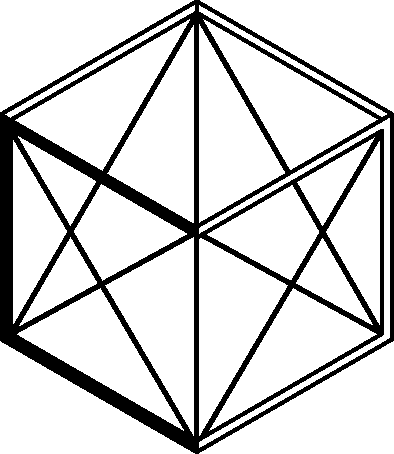
\includegraphics[width=0.28\textwidth]{../documentation/logo/logo-eps-converted-to.pdf}\par
    \vspace{1.2cm}
  }{%
    \vspace{0.8cm}
  }
  {\Huge\bfseries FEMaster User Manual\par}
  \vspace{0.4cm}
  {\large Finite Elements in Mechanical Analysis and Simulation for Technical Engineering Research\par}
  \vfill
  {\large Version 2.6.25\par}
  {\large 19 August 2026\par}
\end{titlepage}

\tableofcontents

\mainmatter
\chapter{Overview}

FEMaster is a finite-element solver for structural mechanics. The same solver-facing model can be constructed from the native FEMaster input language or from the Abaqus input subset implemented by FEMaster. This manual deliberately documents both representations together. The objective is not to teach two unrelated file formats, but to explain the mechanical model once and then show how the same concept is expressed in each input dialect.

The manual is therefore organized by finite-element modelling topic rather than by parser implementation. Model organization and mesh definition come first, followed by regions, materials, sections, coordinate systems, fields, loads, constraints, contact, analysis procedures, numerical controls, and result output. Within these chapters every input keyword has one canonical location. Each keyword begins on a new page and is documented with its purpose, scope, parameters, data-line format, semantic effects, and a side-by-side FEMaster/Abaqus example.

\section{Two input dialects, one model}

The native FEMaster language and the supported Abaqus reader are separate parsers, but both construct the same semantic \emph{Model}. In particular, both readers can construct reusable Parts and rigid Instances. The semantic model is subsequently compiled exactly once into dense solver-facing \emph{ModelData}. Part-local node and element identifiers therefore remain local while the input is being interpreted; instance expansion and deterministic assembly identifiers are created at the compile boundary.

This distinction is useful even for users who never create an explicit \cmd{PART}. A simple flat deck remains the shortest representation for many analyses. FEMaster provides a default model context for such input, so nodes, elements, sets, sections, loads, and analyses can be written without introducing an explicit part/assembly hierarchy. Parts and Instances become useful when the same topology is reused, when local identifiers should remain independent between components, or when a component should be placed repeatedly using rigid translations and rotations.

\begin{notebox}[Optional part/assembly hierarchy]
A model does not need \cmd{PART}, \cmd{ASSEMBLY}, or \cmd{INSTANCE}. Their presence changes model organization and identifier scope, not the fundamental finite-element equations. The flat form is intentionally retained as a first-class FEMaster workflow.
\end{notebox}

\section{Semantic model and compile boundary}

Before compilation, FEMaster stores model topology in semantic objects. A Part owns its local nodes and elements together with part-level regions such as node sets, element sets, and surfaces. An Instance references a Part and carries an affine rigid placement. Materials, profiles, orientations, section descriptions, amplitudes, and analysis definitions remain named model resources.

Compilation flattens the reusable topology into the dense fields required by assembly and solution. Each Instance contributes transformed node coordinates and a corresponding copy of the referenced part topology. Part-level sets and surfaces are expanded for the instance and mapped to the compiled identifiers. Assembly-level regions can then combine entities originating from different instances. The solver works only with the compiled representation; it does not repeatedly interpret part-local identifiers while assembling matrices.

Conceptually, the data flow is

\[
\text{input deck}
\longrightarrow
\text{semantic Model}
\longrightarrow
\operatorname{compile}()
\longrightarrow
\text{dense ModelData}
\longrightarrow
\text{analysis}.
\]

The parser currently evaluates a deck in dependency-ordered complete-file passes so that global definitions, semantic topology, compiled assembly regions, and analyses are created in a deterministic order. This is an implementation mechanism rather than a requirement to manually duplicate or stage an input file. Users should write definitions in a logical readable order; the manual describes observable model semantics rather than relying on parser-pass details.

\section{Model entities}

Nodes define reference positions and provide mechanical degrees of freedom. Elements connect nodes and introduce interpolation, kinematics, and element-specific state. Named node sets and element sets define reusable regions. Surfaces identify element faces or surface collections and are used by pressure loads, distributed loads, ties, couplings, and contact.

Materials define constitutive behaviour and mass density. Sections connect element regions to material and geometric properties such as shell thickness, truss area, or beam profile data. Coordinate systems and orientations define local bases for anisotropy, sections, loads, supports, and nodal transformations. Fields store spatially varying nodal, elemental, element-nodal, integration-point, or material-point information where a model feature requires data beyond a scalar keyword parameter.

Loads and supports are named model objects in native FEMaster input. A loadcase selects the collectors that participate in an analysis. Abaqus input expresses the same high-level idea through Step scopes containing procedures, boundary conditions, and loads. The reader converts supported Abaqus procedures into the corresponding FEMaster loadcase objects.

\section{Supported analysis families}

\begin{longtable}{@{}p{0.30\linewidth}p{0.60\linewidth}@{}}
\toprule
\textbf{FEMaster analysis} & \textbf{Purpose} \\
\midrule
\endhead
\val{LINEARSTATIC} & Small-displacement static equilibrium for the assembled linear system. \\
\val{LINEARSTATICTOPO} & Linear static analysis with element-wise topology density, penalization, and optional material-orientation fields. \\
\val{NONLINEARSTATIC} & Incremental nonlinear equilibrium with load control or arc-length path following, nonlinear element formulations, and nonlinear contact where applicable. \\
\val{EIGENFREQ} & Constrained free-vibration eigenvalue analysis using the assembled stiffness and mass matrices. \\
\val{LINEARBUCKLING} & Linearized buckling analysis based on a preloaded equilibrium state and geometric stiffness. \\
\val{LINEARTRANSIENT} & Implicit linear time integration with Newmark parameters, optional Rayleigh damping, initial velocity, and configurable result cadence. \\
\val{LINEARHARMONIC} & Direct steady-state harmonic response over a specified excitation-frequency sweep with optional Rayleigh damping. \\
\bottomrule
\end{longtable}

The Abaqus reader maps the supported \cmd{STATIC}, \cmd{FREQUENCY}, \cmd{BUCKLE}, \cmd{DYNAMIC}, and \cmd{STEADY STATE DYNAMICS} procedures onto these FEMaster analysis families. Procedure-specific details are documented in Chapter~\ref{chap:analysis-procedures}.

\section{Degree-of-freedom convention}

Mechanical nodal vectors use the order
\[
\text{\dofvec}.
\]
The first three entries are translations and the last three are rotations. This six-component convention is used uniformly by generalized loads, supports, many constraint definitions, and internal nodal fields even when a particular element formulation uses only a subset. Continuum solid elements usually activate translational degrees of freedom only, whereas beams and shells also use rotational components.

\section{Reading the keyword pages}

Each keyword page starts with continuous explanatory text. The following parameter and data-line tables describe the accepted grammar without replacing the explanation of what the command actually does. The final side-by-side block compares the native FEMaster representation with the supported Abaqus representation of the same modelling intent.

When both columns contain identical syntax, that is intentional: it communicates that the input can be written in the same way in both dialects. When no corresponding keyword is implemented in the Abaqus reader, the Abaqus column states that explicitly rather than presenting unsupported Abaqus syntax as if FEMaster could read it. Conversely, Abaqus-only input keywords such as \cmd{BOUNDARY}, \cmd{DSLOAD}, or procedure keywords are documented alongside the native FEMaster mechanism to which they are translated.

\chapter{Build and Command Line}

FEMaster is built with CMake. A typical build produces an executable named \file{FEMaster} in the build output directory. The executable reads an input deck and writes result files using a common job base name. If no explicit output path is supplied, the job base is derived from the input file name. FEMaster then writes both the native text result file \file{.res} and the CalculiX/CGX result file \file{.frd}.

\section{Build}

\begin{shellcmd}
cmake -S . -B build -DCMAKE_BUILD_TYPE=Release
cmake --build build --config Release
\end{shellcmd}

A release build is the normal choice for analysis work. A debug build is useful for small diagnostic models, assertions, and development checks, but it is usually too slow for larger finite-element models.

\section{CMake presets}

The repository provides CMake presets for the common supported toolchain combinations. Presets place their build directory under \file{build/<preset-name>} and set the normal release-oriented defaults: tests disabled, double precision enabled, Eigen compile-time reduction flags enabled, and OpenMP disabled unless the preset explicitly enables it.

\begin{shellcmd}
cmake --preset linux
cmake --build --preset linux

cmake --preset linux-mkl-omp
cmake --build --preset linux-mkl-omp
\end{shellcmd}

The Linux presets cover CPU-only builds, OpenMP builds, oneMKL builds, CUDA builds, cuDSS builds, and combined CUDA/oneMKL configurations. Windows presets are split between MSVC and IntelLLVM toolchains. macOS currently provides CPU presets. The exact preset list should be read from \file{CMakePresets.json} for the checked-out version.

\begin{longtable}{@{}p{0.32\linewidth}p{0.58\linewidth}@{}}
\toprule
\textbf{CMake option} & \textbf{Meaning} \\
\midrule
\endhead
\key{FEMASTER_BUILD_TESTS} & Build and register the GoogleTest executable. \\
\key{FEMASTER_ENABLE_CUDA} & Build CUDA solver backends. \\
\key{FEMASTER_ENABLE_CUDSS} & Use NVIDIA cuDSS for CUDA sparse direct solves. Requires CUDA. \\
\key{FEMASTER_ENABLE_MKL} & Use Intel oneMKL for Eigen operations and PARDISO. \\
\key{FEMASTER_MKL_SEQUENTIAL} & Use the sequential oneMKL threading layer. \\
\key{FEMASTER_MKL_STATIC} & Link oneMKL component libraries statically. \\
\key{FEMASTER_ENABLE_OPENMP} & Enable OpenMP for FEMaster CPU loops. \\
\key{FEMASTER_DOUBLE_PRECISION} & Use double precision arithmetic. \\
\key{FEMASTER_FAST_EIGEN_COMPILE} & Use Eigen compile-time reduction flags. \\
\key{FEMASTER_STATIC_RUNTIME} & Link compiler C/C++ runtimes statically where supported. \\
\key{FEMASTER_FULLY_STATIC} & Produce a fully static Linux executable. Incompatible with CUDA shared libraries. \\
\key{FEMASTER_TIME_REPORT} & Enable compiler timing diagnostics where supported. \\
\key{FEMASTER_DEPS_INCLUDE_DIR} & Include root containing header-only dependencies such as Eigen, Spectra, and argparse. \\
\key{FEMASTER_CUDSS_ROOT} & Root of an NVIDIA cuDSS installation. Defaults to the \key{CUDSS_DIR} environment variable. \\
\bottomrule
\end{longtable}

\section{Running an input deck}

\begin{shellcmd}
FEMaster model.inp
FEMaster model.inp --output model.res
FEMaster model.inp --ncpus 8
\end{shellcmd}

\begin{longtable}{@{}p{0.28\linewidth}p{0.62\linewidth}@{}}
\toprule
\textbf{Argument} & \textbf{Meaning} \\
\midrule
\endhead
\file{input_file} & Path to the input deck. If no \file{.inp} suffix is supplied, it is added automatically. \\
\key{--output FILE} & Explicit output base or result file path. The suffix \file{.res}, \file{.frd}, or \file{.inp} is stripped before writers are opened, so \file{--output run.res} produces \file{run.res} and \file{run.frd}. \\
\key{--ncpus N} & Number of threads allowed for parallel assembly and compute sections. \\
\bottomrule
\end{longtable}

At the end of a regular solver run, FEMaster prints a process timing summary in hours, minutes, seconds, milliseconds, and total milliseconds. This timing covers the full executable run, including parsing, solving, result writing, and shutdown.

\section{DSL documentation mode}

The executable can print DSL registration information for the installed version. This is useful when checking which commands, keywords, and variants a particular build accepts.

\begin{shellcmd}
FEMaster --document --doc-list
FEMaster --document --doc-show CLOAD
FEMaster --document --doc-variants ELASTIC
\end{shellcmd}

\begin{longtable}{@{}p{0.34\linewidth}p{0.56\linewidth}@{}}
\toprule
\textbf{Option} & \textbf{Meaning} \\
\midrule
\endhead
\key{--doc-list} & Print the available DSL commands. \\
\key{--doc-show CMD} & Show details for one command. \\
\key{--doc-tokens CMD} & Show expected tokens for a command. \\
\key{--doc-variants CMD} & Show accepted data-line variants. \\
\key{--doc-search TEXT} & Search command names and descriptions. \\
\key{--doc-where-token TOKEN} & Find commands that use a token. \\
\key{--doc-all} & Print the full command overview. \\
\key{--doc-format text|md|json} & Select the documentation output format. Currently the implementation falls back to text for non-text formats. \\
\key{--doc-verbosity index|compact|full} & Select the detail level for command documentation. \\
\key{--doc-width N} & Set the wrapping width for documentation output. Use 0 for no wrapping. \\
\key{--doc-no-wrap} & Disable wrapping. Equivalent to \key{--doc-width 0}. \\
\key{--doc-regex} & Treat \key{--doc-search} as a regular expression. \\
\bottomrule
\end{longtable}

\chapter{Input Format}

FEMaster reads keyword-based input decks. Both the native FEMaster language and the implemented Abaqus input subset use the familiar form in which a command starts with an asterisk, optional parameters follow after commas, and command-specific data are supplied on one or more subsequent lines. This chapter describes the common lexical and structural rules. The following chapters then document individual commands in their mechanical context.

The two dialects should be understood as two front ends to the same finite-element model. Native FEMaster input exposes FEMaster-specific concepts directly, especially named load/support collectors, explicit loadcases, fields, solver controls, and advanced model features. Abaqus input uses Abaqus-style structural scopes and Step procedure keywords. Where a command is shared, FEMaster intentionally keeps the syntax as close as practical to the Abaqus representation. Where the modelling concepts differ, the side-by-side examples make the translation explicit.

\section{Command lines}

A command line begins with \texttt{*}. The command name follows immediately and may be followed by comma-separated parameters. Parameters can be key/value pairs or flags. Data lines continue until the next command line begins.

\begin{syntax}
*COMMAND, KEY=value, FLAG
value, value, value
value, value, value
\end{syntax}

Command and parameter names are normalized before lookup. Command-name case is therefore not significant, and whitespace inside normalized command names is ignored by the parser. The manual nevertheless writes canonical uppercase spellings because they are easier to scan and correspond to conventional finite-element deck style. For example, the internal command name \val{SOLIDSECTION} is documented and normally written as \cmd{SOLID SECTION} where that form improves readability.

Parameter values preserve their semantic type. Numerical values are parsed as integer or floating-point quantities according to the command grammar. Boolean-style flags may either be present without a value or use explicit values where supported. Names are used to resolve materials, parts, regions, collectors, coordinate systems, fields, and other named resources.

\section{Data lines and multiline records}

The number and meaning of data-line values are command specific. Some commands accept one record per line, such as \cmd{NODE}; others consume a fixed-size matrix or a variable number of identifiers. The parser grammar defines whether a record can span multiple physical lines. The keyword pages in this manual describe data in semantic units rather than requiring users to infer record boundaries from examples.

Comma-separated values are preferred because they remain readable when optional entries are empty. Whitespace around values is ignored. A literal \val{NAN} is used by several native FEMaster commands to express an unconstrained or unspecified generalized component rather than a numerical zero.

\section{Scopes}

Several keywords open structural scopes. A Part scope owns part-local mesh topology and part-level regions. An Assembly scope contains instance placement and assembly-level region definitions. Material subcommands apply to the active material. Native FEMaster \cmd{LOADCASE} opens an analysis context in which subsequent control keywords configure the current analysis. Abaqus \cmd{STEP} opens the corresponding Abaqus analysis context and is terminated by \cmd{END STEP}.

Scopes are semantic rather than indentation based. Indentation can be used for readability, but it has no meaning to the parser. Closing commands such as \cmd{END PART}, \cmd{END ASSEMBLY}, \cmd{END INSTANCE}, \cmd{END STEP}, and the native \cmd{END} make the structural boundary explicit.

\section{Names, identifiers, and references}

Numeric node and element identifiers are local to the topology in which they are defined. In a flat native FEMaster deck this effectively behaves like a single model namespace. Inside an explicit Part, identifiers are part-local and may therefore be reused by another Part. An Instance does not renumber the source Part. During \texttt{Model::compile()} each instance receives deterministic maps from local identifiers to dense compiled assembly identifiers.

Named resources provide the stable user-facing references used by the remainder of a deck. Node sets, element sets, surfaces, materials, profiles, orientations, fields, amplitudes, collectors, and loadcases are referenced by name. Assembly-level region syntax may qualify a part-local or instance-local entity where required by the grammar. The region chapter documents these cases in detail.

\section{Definition order and parser passes}

The current readers replay the input in dependency-ordered passes. Shared definitions such as materials and orientations are collected before semantic topology is constructed. Parts and Instances are then built, the model is compiled exactly once, assembly regions and compiled fields are materialized, and the final pass creates loads, constraints, and analyses. The Abaqus reader follows the same broad lifecycle.

This implementation permits definitions that are resolved in an earlier semantic pass to be written in a natural deck order without forcing the solver to retain sparse deck identifiers internally. It does not mean that arbitrary forward references are equally meaningful. A deck should still be written so that a human reader encounters a definition before the feature that conceptually depends on it whenever possible. In particular, field-driven features should place the \cmd{FIELD} definition before the command that selects the field.

\begin{implementationnote}[Compile boundary]
The important user-visible rule is that Part topology is reusable and sparse before compilation, while assembly-dependent operations work on the compiled model. The number of internal parser passes is not an input-language feature and should not be used as a mechanism for intentionally obscure deck ordering.
\end{implementationnote}

\section{FEMaster and Abaqus presentation in this manual}

Every keyword page contains a two-column example. The left column always shows the native FEMaster representation. The right column shows input accepted by the supported Abaqus reader when such a representation exists. If both dialects intentionally share the same command, both columns show it. If the Abaqus reader does not implement an equivalent command, the right column states this explicitly. This avoids conflating general Abaqus capabilities with the subset that FEMaster actually reads.

\keywordpage{HEADING}

\cmd{HEADING} attaches descriptive text to an input deck. It does not alter the finite-element model, equation system, or result values. The command is useful for keeping exported or archived decks self-describing and is accepted by both readers. Because heading text is metadata, no later command references it by name.

The heading is intentionally treated as an input-language concern rather than as a model entity. It may appear at root level and should normally be placed near the beginning of the file. Multiple physical words or punctuation can be used in the heading data according to the command grammar; the text is not interpreted as numerical model data.

\syntaxheading

\begin{syntax}
*HEADING
Descriptive model title
\end{syntax}

There are no mechanical parameters. The following data text is retained only as descriptive deck information. A heading is optional.

\exampleheading

\begin{dialectexamples}
\begin{femasterdeck}
*HEADING
Cantilever verification model
\end{femasterdeck}
\begin{abaqusdeck}
*HEADING
Cantilever verification model
\end{abaqusdeck}
\end{dialectexamples}

\notesheading

Do not use \cmd{HEADING} as a model name or as a substitute for a Part, Assembly, loadcase, or output identifier. Native FEMaster also accepts \cmd{MODEL, NAME=...} as an optional explicit root marker; that command has structural semantics and is documented in the Model Definition chapter.

\chapter{Model Definition}
\label{chap:model-definition}

Model definition describes the geometry and topology on which the analysis is built. A simple FEMaster model may be completely flat: nodes and elements can be defined directly without an explicit Part, Assembly, or Instance. The structured Part/Assembly form is optional and becomes useful when components are reused, when the same Part is placed more than once, when separate local ID spaces are desirable, or when an Abaqus-style assembly is imported.

From the user's point of view, the two forms describe the same kind of finite-element model. In a flat model there is one direct topology. In a structured model, each Part owns its local nodes, elements, sets, surfaces, and section assignments, while Instances place those Parts into the final assembly. Parts therefore describe \emph{what a component is}; Instances describe \emph{where that component is}.

Node and element IDs are user labels. They are non-negative integers, may start at \textbf{0}, and may be sparse. Separate Parts may reuse the same numerical IDs because their topologies are independent. When an assembly-level definition needs to distinguish entities belonging to different Instances, the Instance name provides the required qualification.

\section{Model organization}

\keywordpage{MODEL}

\cmd{MODEL} is an optional native FEMaster root marker. It can attach a descriptive model name to a native deck and makes the top-level structure explicit, but it is not required. A file may begin directly with nodes, materials, Parts, or other root-level definitions.

\key{NAME} is optional. The command does not create a nested second model and is not used to select between several models in one input file. Use \cmd{HEADING} for free descriptive text and \cmd{MODEL} when an explicit native model marker improves readability.

\begin{keywordparameters}
\key{NAME} & optional & Descriptive name of the native FEMaster model. \\
\end{keywordparameters}

\syntaxheading

\begin{syntax}
*MODEL, NAME=BRACKET_MODEL
\end{syntax}

No data lines follow \cmd{MODEL}.

\exampleheading

\begin{dialectexamples}
\begin{femasterdeck}
*MODEL, NAME=BRACKET_MODEL
*NODE
0, 0., 0., 0.
1, 10., 0., 0.
\end{femasterdeck}
\begin{abaqusdeck}
** No MODEL wrapper is required.
*NODE
0, 0., 0., 0.
1, 10., 0., 0.
\end{abaqusdeck}
\end{dialectexamples}

\notesheading

\cmd{MODEL} is optional even when no explicit \cmd{PART} is used. It should not be confused with \cmd{PART}: a Part creates a reusable topology and its own local ID space, while \cmd{MODEL} is only the optional top-level native marker.

\keywordpage{PART}

\cmd{PART} begins a reusable finite-element component definition. Nodes, elements, part-level sets, surfaces, and section assignments that follow belong to the active Part until \cmd{END PART} closes it.

A Part is defined in its own local coordinate system. Its node coordinates describe the undeformed component geometry before any Instance placement. The Part itself has no global translation or rotation. If the same component is needed in several locations, define its topology once and create several \cmd{INSTANCE} entries.

Part-local IDs are independent. Node \val{0} in Part \val{LEFT} and node \val{0} in Part \val{RIGHT} are different nodes even though they use the same numerical label. The same applies to element IDs. This is one of the main practical advantages of the Part representation: imported or reusable components do not need to be renumbered merely because another Part uses the same IDs.

Explicit Parts are optional in native FEMaster input. If nodes and elements are written directly at root level, they belong to the flat model topology and can be used without writing \cmd{PART}, \cmd{ASSEMBLY}, or \cmd{INSTANCE}.

\begin{keywordparameters}
\key{NAME} & required & Unique Part name. The name is referenced by \cmd{INSTANCE}. \\
\end{keywordparameters}

No data line belongs directly to \cmd{PART}; the Part body consists of nested model-definition commands.

\exampleheading

\begin{dialectexamples}
\begin{femasterdeck}
*PART, NAME=ROD
*NODE, NSET=PNODES
0,   0., 0., 0.
1, 100., 0., 0.
*ELEMENT, TYPE=T3, ELSET=BAR
0, 0, 1
*END PART
\end{femasterdeck}
\begin{abaqusdeck}
*PART, NAME=ROD
*NODE, NSET=PNODES
0,   0., 0., 0.
1, 100., 0., 0.
*ELEMENT, TYPE=T3D2, ELSET=BAR
0, 0, 1
*END PART
\end{abaqusdeck}
\end{dialectexamples}

\notesheading

Part-level sets, surfaces, materials assigned through sections, and other part-level definitions follow the Part when it is instantiated. Define properties that belong to the component itself at Part level; define selections that combine several placed components at Assembly level.

\keywordpage{END PART}

\cmd{END PART} closes the active Part scope. It takes no parameters and no data lines. Definitions that follow are no longer part-local unless another \cmd{PART} is opened.

\syntaxheading

\begin{syntax}
*END PART
\end{syntax}

\exampleheading

\begin{dialectexamples}
\begin{femasterdeck}
*PART, NAME=PLATE
...
*END PART
\end{femasterdeck}
\begin{abaqusdeck}
*PART, NAME=PLATE
...
*END PART
\end{abaqusdeck}
\end{dialectexamples}

\notesheading

Do not use native \cmd{END} as a replacement for \cmd{END PART}. \cmd{END} terminates a native loadcase, whereas \cmd{END PART} closes a Part definition.

\keywordpage{ASSEMBLY}

\cmd{ASSEMBLY} begins the optional Assembly scope. The Assembly is where placed Instances and regions that refer to the assembled model are defined. A model that does not need explicit Instances may omit this scope entirely.

The Assembly is especially useful when several Parts are combined or one Part is repeated. Part-level topology remains expressed with local IDs, while Assembly-level sets and surfaces can select entities from particular Instances. This allows the model to preserve meaningful local numbering inside each component without forcing a single manually renumbered global mesh.

\key{NAME} is optional and defaults to \val{ASSEMBLY}. The name is descriptive for the supported current workflow; the important user-visible objects inside the Assembly are the Instances and assembly-level regions.

\begin{keywordparameters}
\key{NAME} & optional & Assembly name; default \val{ASSEMBLY}. \\
\end{keywordparameters}

\exampleheading

\begin{dialectexamples}
\begin{femasterdeck}
*ASSEMBLY, NAME=ASSEMBLY
*INSTANCE, NAME=ROD_A, PART=ROD
0., 0., 0.
*END INSTANCE
*END ASSEMBLY
\end{femasterdeck}
\begin{abaqusdeck}
*ASSEMBLY, NAME=ASSEMBLY
*INSTANCE, NAME=ROD_A, PART=ROD
0., 0., 0.
*END INSTANCE
*END ASSEMBLY
\end{abaqusdeck}
\end{dialectexamples}

\notesheading

Use an Assembly because it improves the physical organization of the model, not because the solver requires one. A flat native model remains the simplest and clearest representation for many single-component analyses.

\keywordpage{END ASSEMBLY}

\cmd{END ASSEMBLY} closes the Assembly scope. It has no parameters and no data lines.

\syntaxheading

\begin{syntax}
*END ASSEMBLY
\end{syntax}

\exampleheading

\begin{dialectexamples}
\begin{femasterdeck}
*ASSEMBLY
...
*END ASSEMBLY
\end{femasterdeck}
\begin{abaqusdeck}
*ASSEMBLY, NAME=ASSEMBLY
...
*END ASSEMBLY
\end{abaqusdeck}
\end{dialectexamples}

\keywordpage{INSTANCE}

\cmd{INSTANCE} places an existing Part in the Assembly. Native FEMaster intentionally accepts the same placement representation used by the supported Abaqus reader. \key{NAME} gives the Instance a unique assembly name and \key{PART} selects the reusable Part.

An Instance may be placed by translation, rotation, both, or neither. A three-value data line gives a translation
\[
\boldsymbol t=(t_x,t_y,t_z).
\]
A seven-value line defines a rotation by two points on the rotation axis and an angle in degrees:
\[
(x_1,y_1,z_1,x_2,y_2,z_2,\varphi).
\]
The two axis points must be distinct. If both translation and rotation are supplied, the translation is applied first and the axis-angle rotation second. With no placement data the Part is instantiated in its original position.

Instance placement changes the position and orientation of the component in the assembled model; it does not require the Part coordinates or Part IDs to be rewritten. Several Instances may therefore reference the same Part with different placements.

\begin{keywordparameters}
\key{NAME} & required & Unique Instance name used for assembly-level references. \\
\key{PART} & required & Name of the Part to place. \\
\end{keywordparameters}

\begin{keyworddata}
\val{tx, ty, tz} & Optional translation vector. \\
\val{x1,y1,z1,x2,y2,z2,angle} & Optional rotation axis through two points and rotation angle in degrees. \\
\end{keyworddata}

\exampleheading

\begin{dialectexamples}
\begin{femasterdeck}
*INSTANCE, NAME=RIGHT, PART=BRACKET
100., 0., 0.
0., 0., 0., 0., 0., 1., 90.
*END INSTANCE
\end{femasterdeck}
\begin{abaqusdeck}
*INSTANCE, NAME=RIGHT, PART=BRACKET
100., 0., 0.
0., 0., 0., 0., 0., 1., 90.
*END INSTANCE
\end{abaqusdeck}
\end{dialectexamples}

\notesheading

Because the Part remains reusable, its local node and element labels remain meaningful in every Instance. Assembly-level sets can select a particular Instance when the same local ID appears in several placed copies.

\keywordpage{END INSTANCE}

\cmd{END INSTANCE} closes the current Instance definition. It takes no parameters or data lines.

\exampleheading

\begin{dialectexamples}
\begin{femasterdeck}
*INSTANCE, NAME=A, PART=BLOCK
20., 0., 0.
*END INSTANCE
\end{femasterdeck}
\begin{abaqusdeck}
*INSTANCE, NAME=A, PART=BLOCK
20., 0., 0.
*END INSTANCE
\end{abaqusdeck}
\end{dialectexamples}

\section{Mesh definition}

\keywordpage{NODE}

\cmd{NODE} defines finite-element nodes by user ID and Cartesian reference coordinates. In a Part scope the nodes belong to that Part. In a flat native model they belong directly to the model topology.

Node IDs are non-negative integers. \textbf{ID 0 is valid.} IDs need not be contiguous and may be chosen to preserve meaningful numbering from a mesh generator or external model. They must only be unique within the topology scope in which they are defined.

The optional \key{NSET} parameter adds every node in the block to a node set. Native FEMaster defaults this set to \val{NALL}. Coordinates are Cartesian reference coordinates. Missing trailing coordinate components default to zero, although explicitly writing all three values is generally clearer in shared examples.

Node order has no mechanical meaning by itself, but the order in which node IDs appear in an element connectivity is crucial because it determines the element's local topology and orientation.

\begin{keywordparameters}
\key{NSET} & optional & Node set receiving all nodes in the block; native default \val{NALL}. \\
\end{keywordparameters}

\begin{keyworddata}
\val{id} & Non-negative user node ID; \val{0} is valid. \\
\val{x, y, z} & Cartesian reference coordinates. \\
\end{keyworddata}

\exampleheading

\begin{dialectexamples}
\begin{femasterdeck}
*NODE, NSET=EDGE
0,  0., 0., 0.
10, 25., 0., 0.
20, 50., 0., 0.
\end{femasterdeck}
\begin{abaqusdeck}
*NODE, NSET=EDGE
0,  0., 0., 0.
10, 25., 0., 0.
20, 50., 0., 0.
\end{abaqusdeck}
\end{dialectexamples}

\notesheading

The coordinates define the undeformed geometry. Loads, prescribed displacements, initial velocities, and Instance placement do not change the meaning of the node's Part-local reference coordinates.

\keywordpage{ELEMENT}

\cmd{ELEMENT} defines element connectivity. Every data record begins with a user element ID followed by the node IDs in the formulation-specific connectivity order. \key{TYPE} selects the finite-element formulation. \key{ELSET} optionally adds all elements in the block to an element set and defaults to \val{EALL} in native FEMaster input.

Element IDs are non-negative user labels and may also begin at \textbf{0}. They may be sparse. Connectivity is written using node IDs from the same topology scope as the element. The connectivity order determines local edges and faces, shell normal direction, solid face labels, element orientation, and the mapping from the reference element to the physical geometry.

The complete formulation reference is given in Chapter~\ref{chap:elements}. That chapter documents the supported solid, shell, beam, and truss elements individually, including node ordering, numerical behaviour, recommended use, and the existing element schematics.

The native and Abaqus input names are not always identical. The solid labels \val{C3D4}, \val{C3D5}, \val{C3D6}, \val{C3D8}, \val{C3D8R}, \val{C3D10}, \val{C3D15}, \val{C3D20}, and \val{C3D20R} are shared. Native \val{T3} corresponds to Abaqus \val{T3D2}. Abaqus shell labels \val{S3/S3R}, \val{S4/S4R}, \val{S6/S6R}, and \val{S8/S8R} are read into the corresponding finite-rotation shell formulations. Native FEMaster additionally exposes the legacy shell types, MITC variants, FRT names, and \val{QSPT} directly.

\begin{keywordparameters}
\key{TYPE} & required & Element formulation/type identifier. \\
\key{ELSET} & optional & Element set receiving all elements in the block; native default \val{EALL}. \\
\end{keywordparameters}

\begin{keyworddata}
\val{id} & Non-negative user element ID; \val{0} is valid. \\
\val{n1, n2, ...} & Node connectivity in the formulation-specific order. \\
\end{keyworddata}

\exampleheading

\begin{dialectexamples}
\begin{femasterdeck}
*ELEMENT, TYPE=T3, ELSET=BARS
0, 0, 10
1, 10, 20

*ELEMENT, TYPE=MITC4FRT, ELSET=PANEL
10, 100, 110, 120, 130
\end{femasterdeck}
\begin{abaqusdeck}
*ELEMENT, TYPE=T3D2, ELSET=BARS
0, 0, 10
1, 10, 20

*ELEMENT, TYPE=S4, ELSET=PANEL
10, 100, 110, 120, 130
\end{abaqusdeck}
\end{dialectexamples}

\notesheading

An element definition provides topology and kinematics, not the complete physical properties. Solids, shells, beams, and trusses require the corresponding section definitions before they have the intended material and geometric stiffness. The element chapter should therefore be read together with Chapter~\ref{chap:sections}.

\chapter{Elements}
\label{chap:elements}

Elements define how the displacement field is interpolated between nodes and therefore determine the kinematic approximation used by the finite-element model. The element formulation controls which deformation modes can be represented, how strains and curvatures are evaluated, how numerical integration is performed, and which result quantities can be recovered. Choosing an appropriate element family is therefore as important as choosing a sufficiently fine mesh.

This chapter documents the element formulations that are currently accepted by FEMaster. It is intentionally more detailed than the \cmd{ELEMENT} keyword page in Chapter~\ref{chap:model-definition}: the keyword page explains how elements are entered, while this chapter explains what the individual formulations represent, how they behave numerically, and when they should be used.

Element IDs are non-negative user labels and may start at \val{0}. Connectivity order is significant. It determines the reference orientation, element faces, shell normals, and the mapping between the reference element and the physical geometry. Always preserve the documented node order when importing or generating meshes.

\section{Supported element types}

\begin{longtable}{@{}p{0.17\linewidth}p{0.11\linewidth}p{0.61\linewidth}@{}}
\toprule
\textbf{FEMaster type} & \textbf{Nodes} & \textbf{Formulation} \\
\midrule
\endhead
\val{C3D4} & 4 & Linear tetrahedral solid. \\
\val{C3D5} & 5 & Five-node pyramid input represented by a degenerated hexahedral topology. \\
\val{C3D6} & 6 & Linear wedge solid. \\
\val{C3D8} & 8 & Linear fully integrated hexahedral solid. \\
\val{C3D8R} & 8 & Reduced-integration hexahedral solid with hourglass stabilization. \\
\val{C3D10} & 10 & Quadratic tetrahedral solid. \\
\val{C3D15} & 15 & Quadratic wedge solid. \\
\val{C3D20} & 20 & Quadratic hexahedral solid with full stiffness integration. \\
\val{C3D20R} & 20 & Quadratic hexahedral solid with reduced stiffness integration. \\
\val{S3} & 3 & Legacy three-node triangular shell. \\
\val{S4} & 4 & Legacy four-node quadrilateral shell. \\
\val{MITC4} & 4 & Legacy four-node MITC shell with tied transverse shear interpolation. \\
\val{S6} & 6 & Legacy six-node quadratic triangular shell. \\
\val{S8} & 8 & Legacy eight-node quadratic quadrilateral shell. \\
\val{MITC8} & 8 & Legacy eight-node MITC shell with tied transverse shear interpolation. \\
\val{MITC3FRT} & 3 & Three-node finite-rotation shell. \\
\val{MITC4FRT} & 4 & Four-node finite-rotation MITC shell. \\
\val{MITC6FRT} & 6 & Six-node finite-rotation MITC shell. \\
\val{MITC8FRT} & 8 & Eight-node finite-rotation MITC shell. \\
\val{QSPT} & 4 & Specialized quadrilateral shear-panel element. \\
\val{B33} & 2 & Three-dimensional beam element. \\
\val{T3} & 2 & Three-dimensional truss element. \\
\bottomrule
\end{longtable}

The Abaqus reader accepts the same solid names \val{C3D4}, \val{C3D5}, \val{C3D6}, \val{C3D8}, \val{C3D8R}, \val{C3D10}, \val{C3D15}, \val{C3D20}, and \val{C3D20R}. Abaqus \val{T3D2} is mapped to FEMaster \val{T3}. Abaqus \val{B33} is mapped to FEMaster \val{B33}. Abaqus shell names are translated as shown below.

\begin{table}[H]
\centering
\begin{tabular}{@{}lll@{}}
\toprule
\textbf{Abaqus input} & \textbf{FEMaster formulation} & \textbf{Comment} \\
\midrule
\val{S3}, \val{S3R} & \val{MITC3FRT} & Both imported labels use the finite-rotation triangular shell. \\
\val{S4}, \val{S4R} & \val{MITC4FRT} & Both imported labels use the finite-rotation four-node MITC shell. \\
\val{S6}, \val{S6R} & \val{MITC6FRT} & Both imported labels use the finite-rotation six-node shell. \\
\val{S8}, \val{S8R} & \val{MITC8FRT} & Both imported labels use the finite-rotation eight-node shell. \\
\bottomrule
\end{tabular}
\caption{Current Abaqus shell-type mapping.}
\end{table}

This mapping is important: an Abaqus \val{S4} deck does \emph{not} select the native legacy \val{S4} formulation. It is translated to \val{MITC4FRT}. Native FEMaster input can still select the legacy shell names explicitly for comparison and regression work.

\section{Solid elements}

Solid elements model a three-dimensional continuum. They use translational nodal degrees of freedom and obtain their constitutive response from a \cmd{SOLID SECTION}. They are appropriate when the full three-dimensional stress state matters, when through-thickness stresses are required, or when local geometry and load introduction cannot be represented adequately by shells or line elements.

Low-order solids are inexpensive but may require significant refinement in bending-dominated problems. Higher-order solids generally represent curvature and stress gradients more efficiently, but they contain more degrees of freedom per element and are more sensitive to poor midside-node placement and distorted mappings. Mesh quality remains essential for every formulation.

\clearpage
\section{\val{C3D4}: 4-node tetrahedral solid}

\begin{figure}[H]
    \centering
    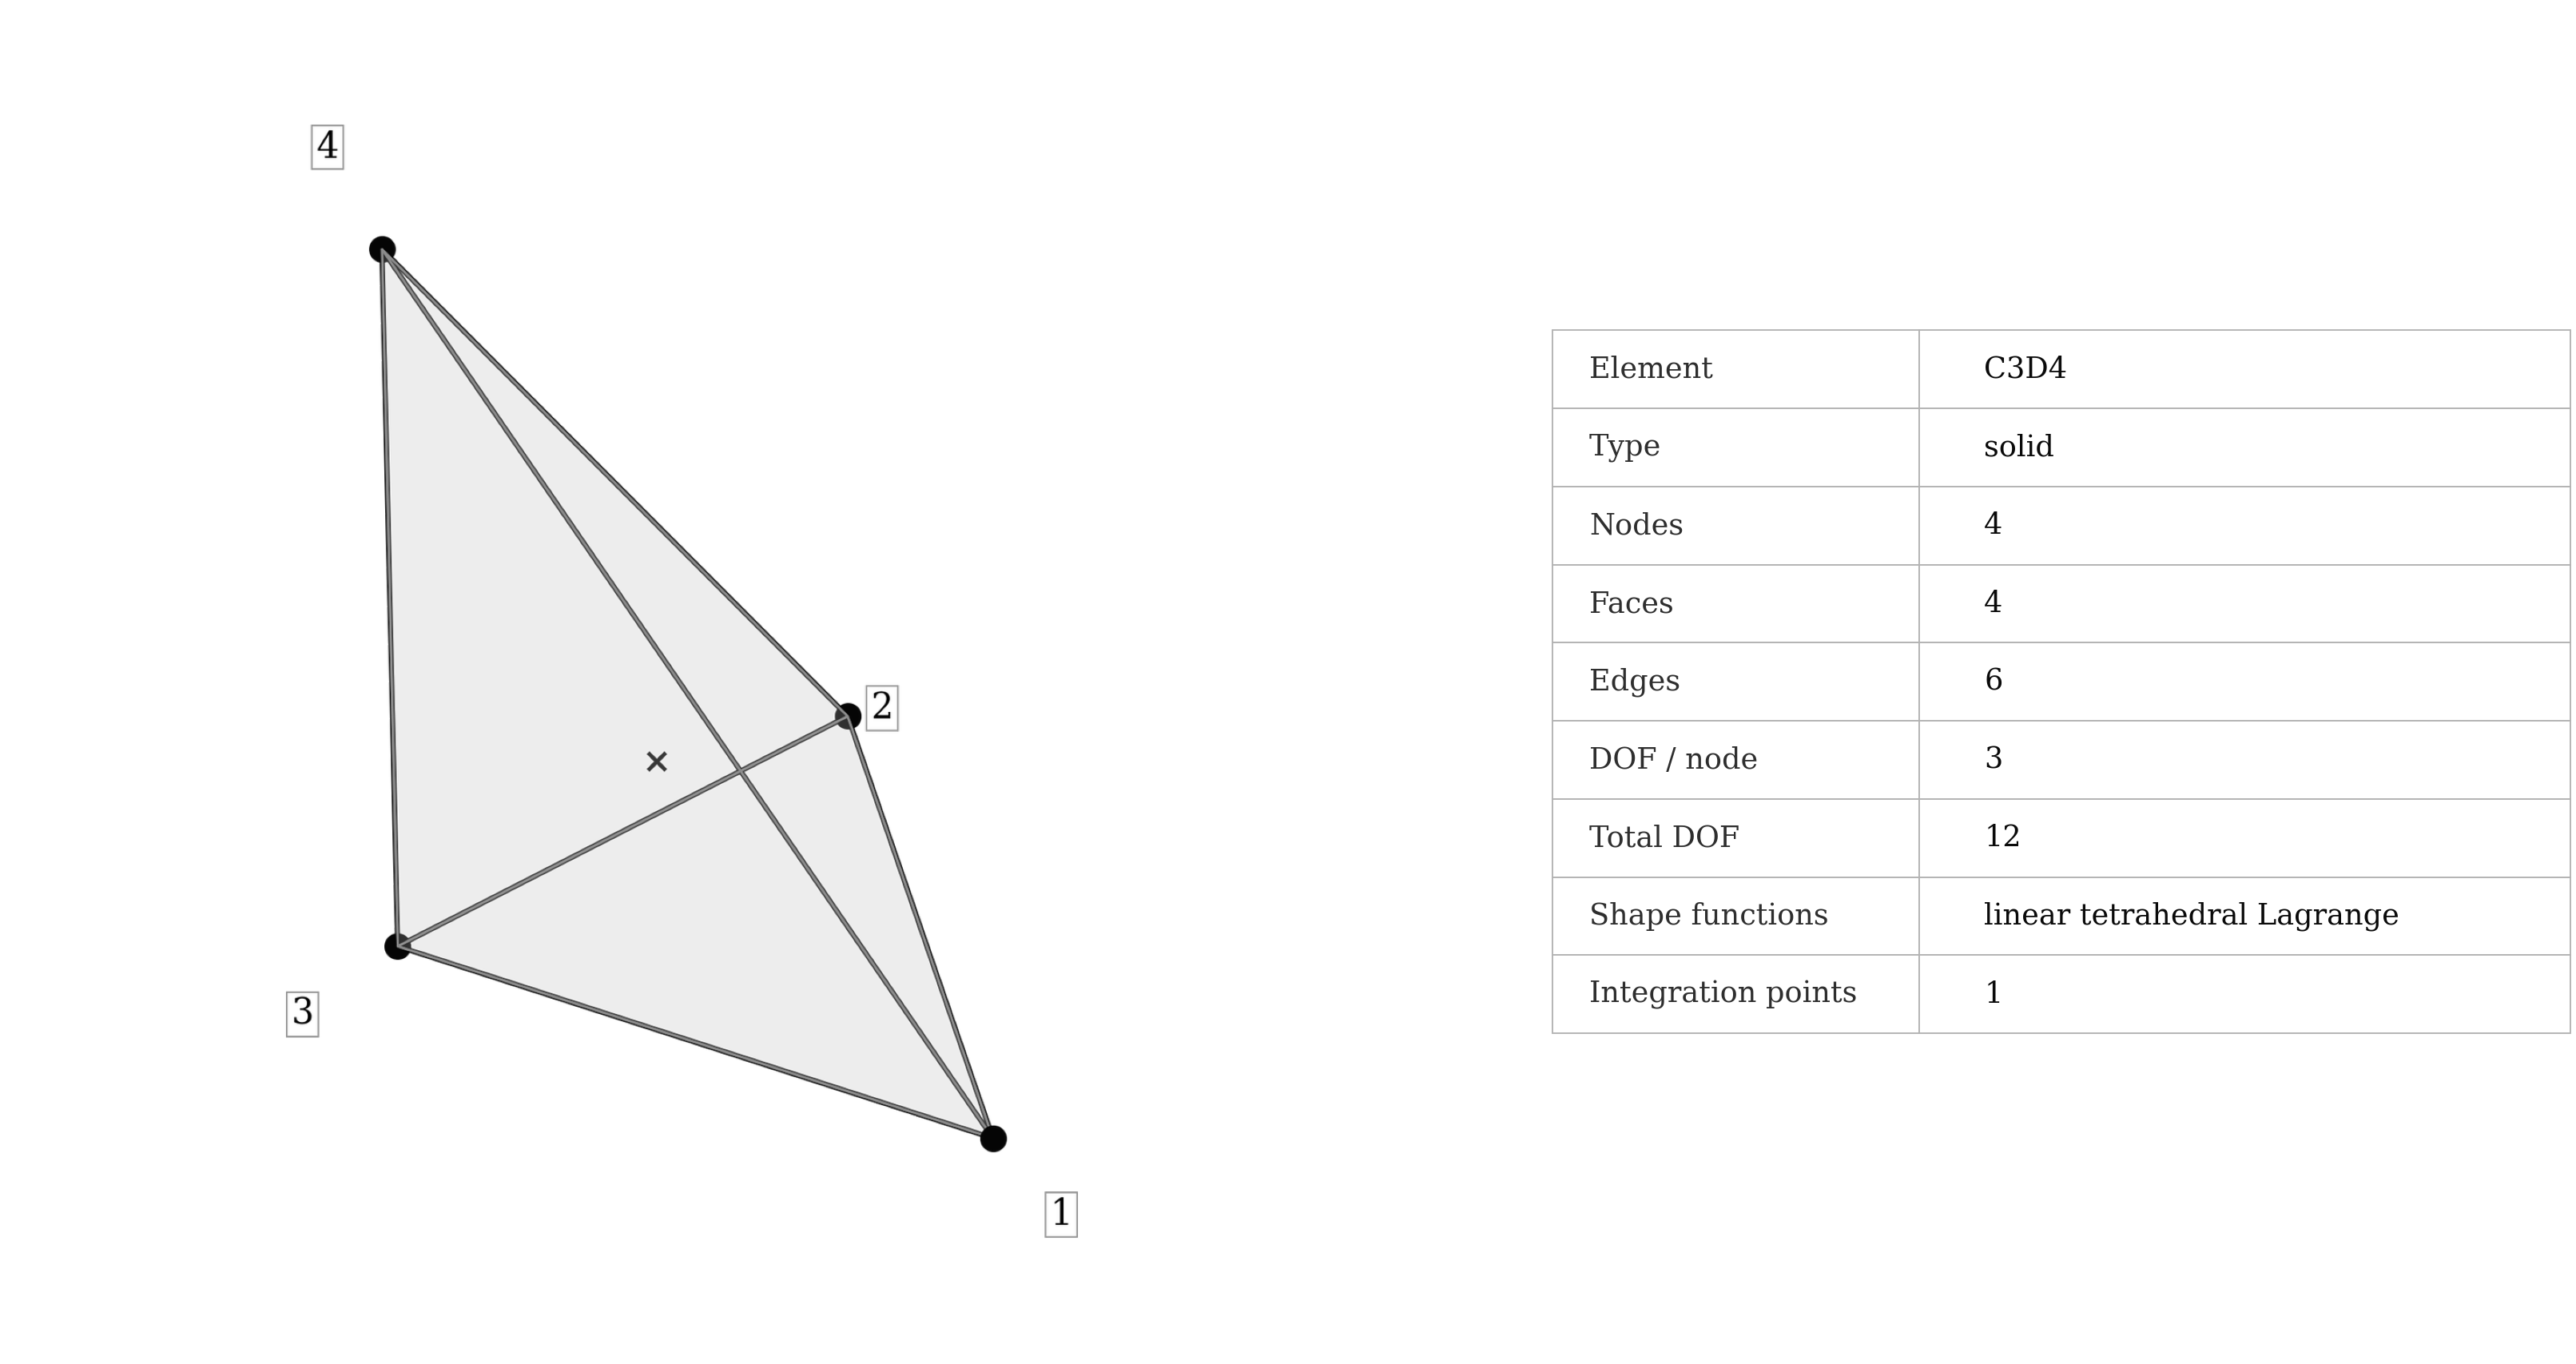
\includegraphics[width=0.78\linewidth]{pages/figures/element_schematics/c3d4_schematic.png}
    \caption{\val{C3D4} element topology and integration scheme.}
\end{figure}

\begin{syntax}
*ELEMENT, TYPE=C3D4, ELSET=<set>
<id>, <n1>, <n2>, <n3>, <n4>
\end{syntax}

\val{C3D4} is the simplest three-dimensional continuum element in FEMaster. It uses four corner nodes and linear displacement interpolation over a tetrahedral reference domain. The resulting strain field is constant within one element, which makes the element inexpensive and geometrically easy to mesh but limits the deformation and stress gradients that a single element can reproduce.

The principal advantage of \val{C3D4} is meshing flexibility. Tetrahedra can fill complex CAD volumes, narrow transitions, and irregular local details with little manual topology design. This makes \val{C3D4} useful for early stiffness checks, coarse load-path studies, and models where robust automatic meshing is more important than stress accuracy per degree of freedom.

The limitation is stiffness and stress resolution. Linear tetrahedra tend to be overly stiff in bending-dominated problems unless the mesh is fine. Since the strain state is constant in each element, stress fields can appear piecewise constant or patchy and steep gradients near holes, fillets, notches, and concentrated loads require substantial refinement.

For stress-sensitive tetrahedral models, \val{C3D10} is usually the better choice. If \val{C3D4} is used, check convergence of displacements, reactions, strain energy, and relevant averaged stresses rather than relying on a single coarse local peak.

\clearpage
\section{\val{C3D5}: 5-node pyramid input}

\begin{figure}[H]
    \centering
    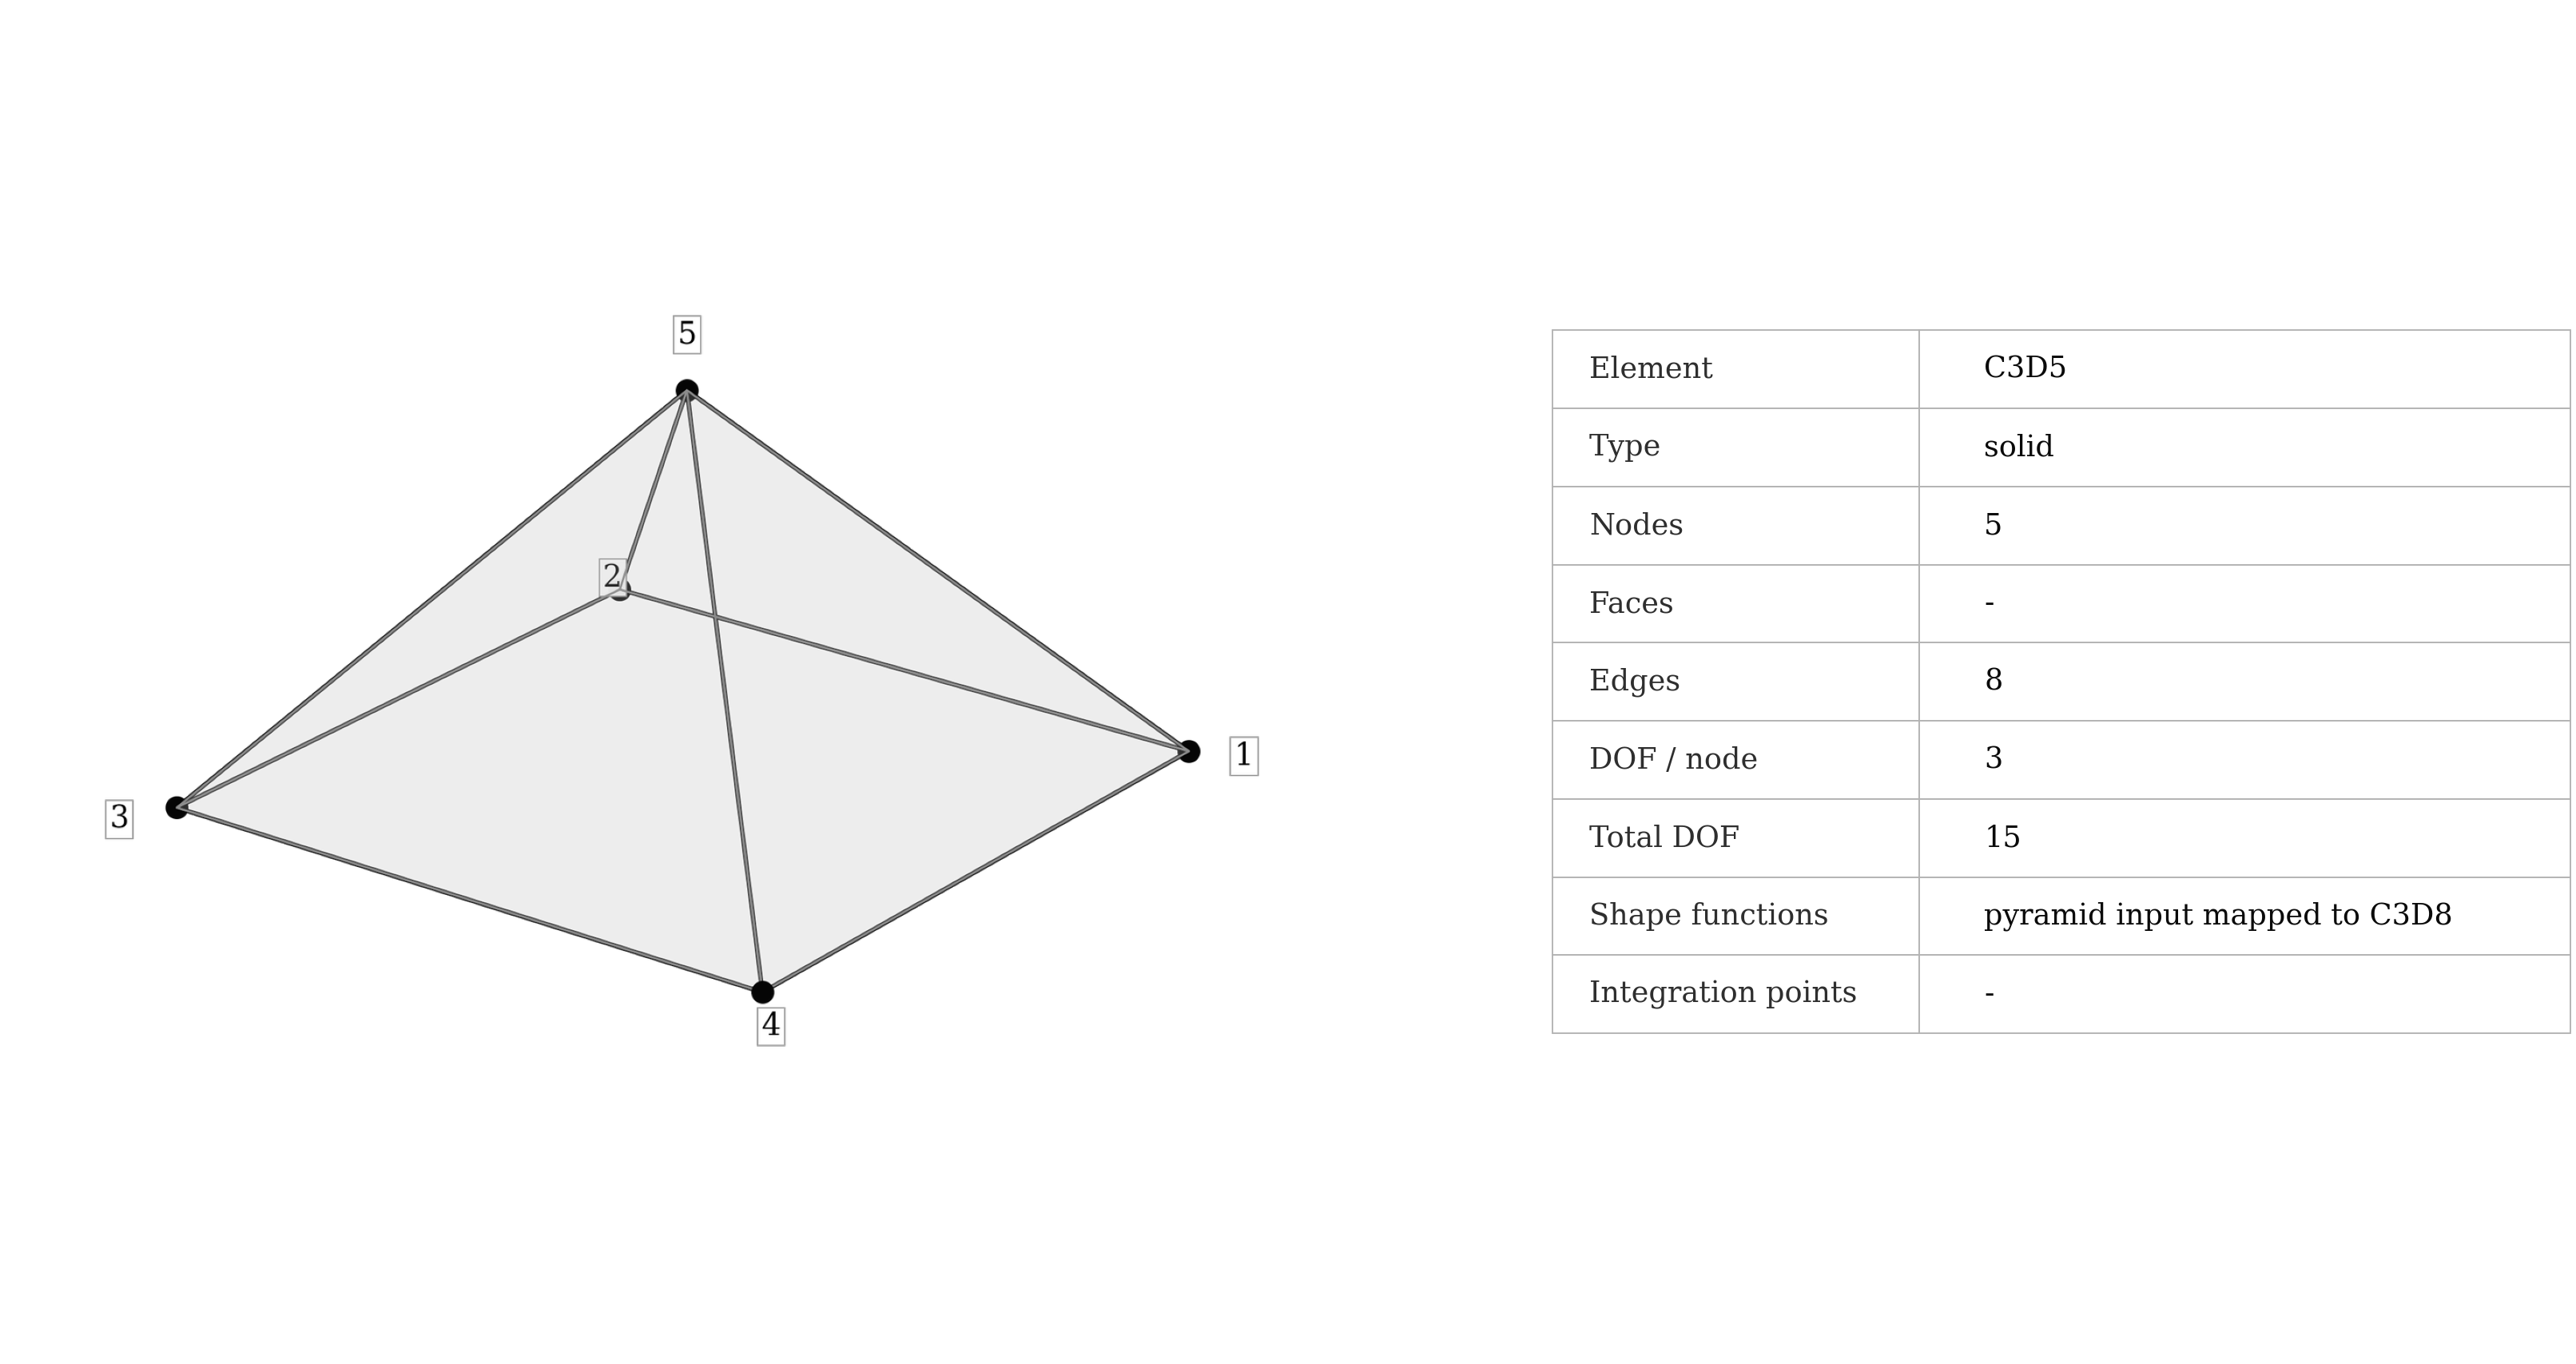
\includegraphics[width=0.78\linewidth]{pages/figures/element_schematics/c3d5_schematic.png}
    \caption{\val{C3D5} pyramid input topology.}
\end{figure}

\begin{syntax}
*ELEMENT, TYPE=C3D5, ELSET=<set>
<id>, <n1>, <n2>, <n3>, <n4>, <apex>
\end{syntax}

\val{C3D5} provides a five-node pyramid connectivity for transition meshes. FEMaster represents this input with a degenerated eight-node hexahedral topology in which the four upper hexahedral positions coincide at the pyramid apex. The user nevertheless writes the natural five-node pyramid connectivity shown above.

The element is primarily useful as a transition cell between hexahedral and tetrahedral regions. This is common in automatically generated mixed meshes where a quadrilateral face must transition toward tetrahedral topology. In such cases a small number of pyramids can preserve mesh compatibility without forcing a large surrounding region to change element family.

A degenerated mapping is generally less predictable than a regular hexahedron, wedge, or tetrahedron. Flat pyramids, badly skewed bases, and apex positions close to the base plane can produce poor Jacobians and unreliable stiffness. Treat \val{C3D5} as a transition element rather than as the preferred element for a large stress-critical volume.

When a model contains many pyramids in the primary load path, compare the result with an alternative mesh. Reactions and global stiffness may remain plausible even when local stress quality has deteriorated.

\clearpage
\section{\val{C3D6}: 6-node wedge solid}

\begin{figure}[H]
    \centering
    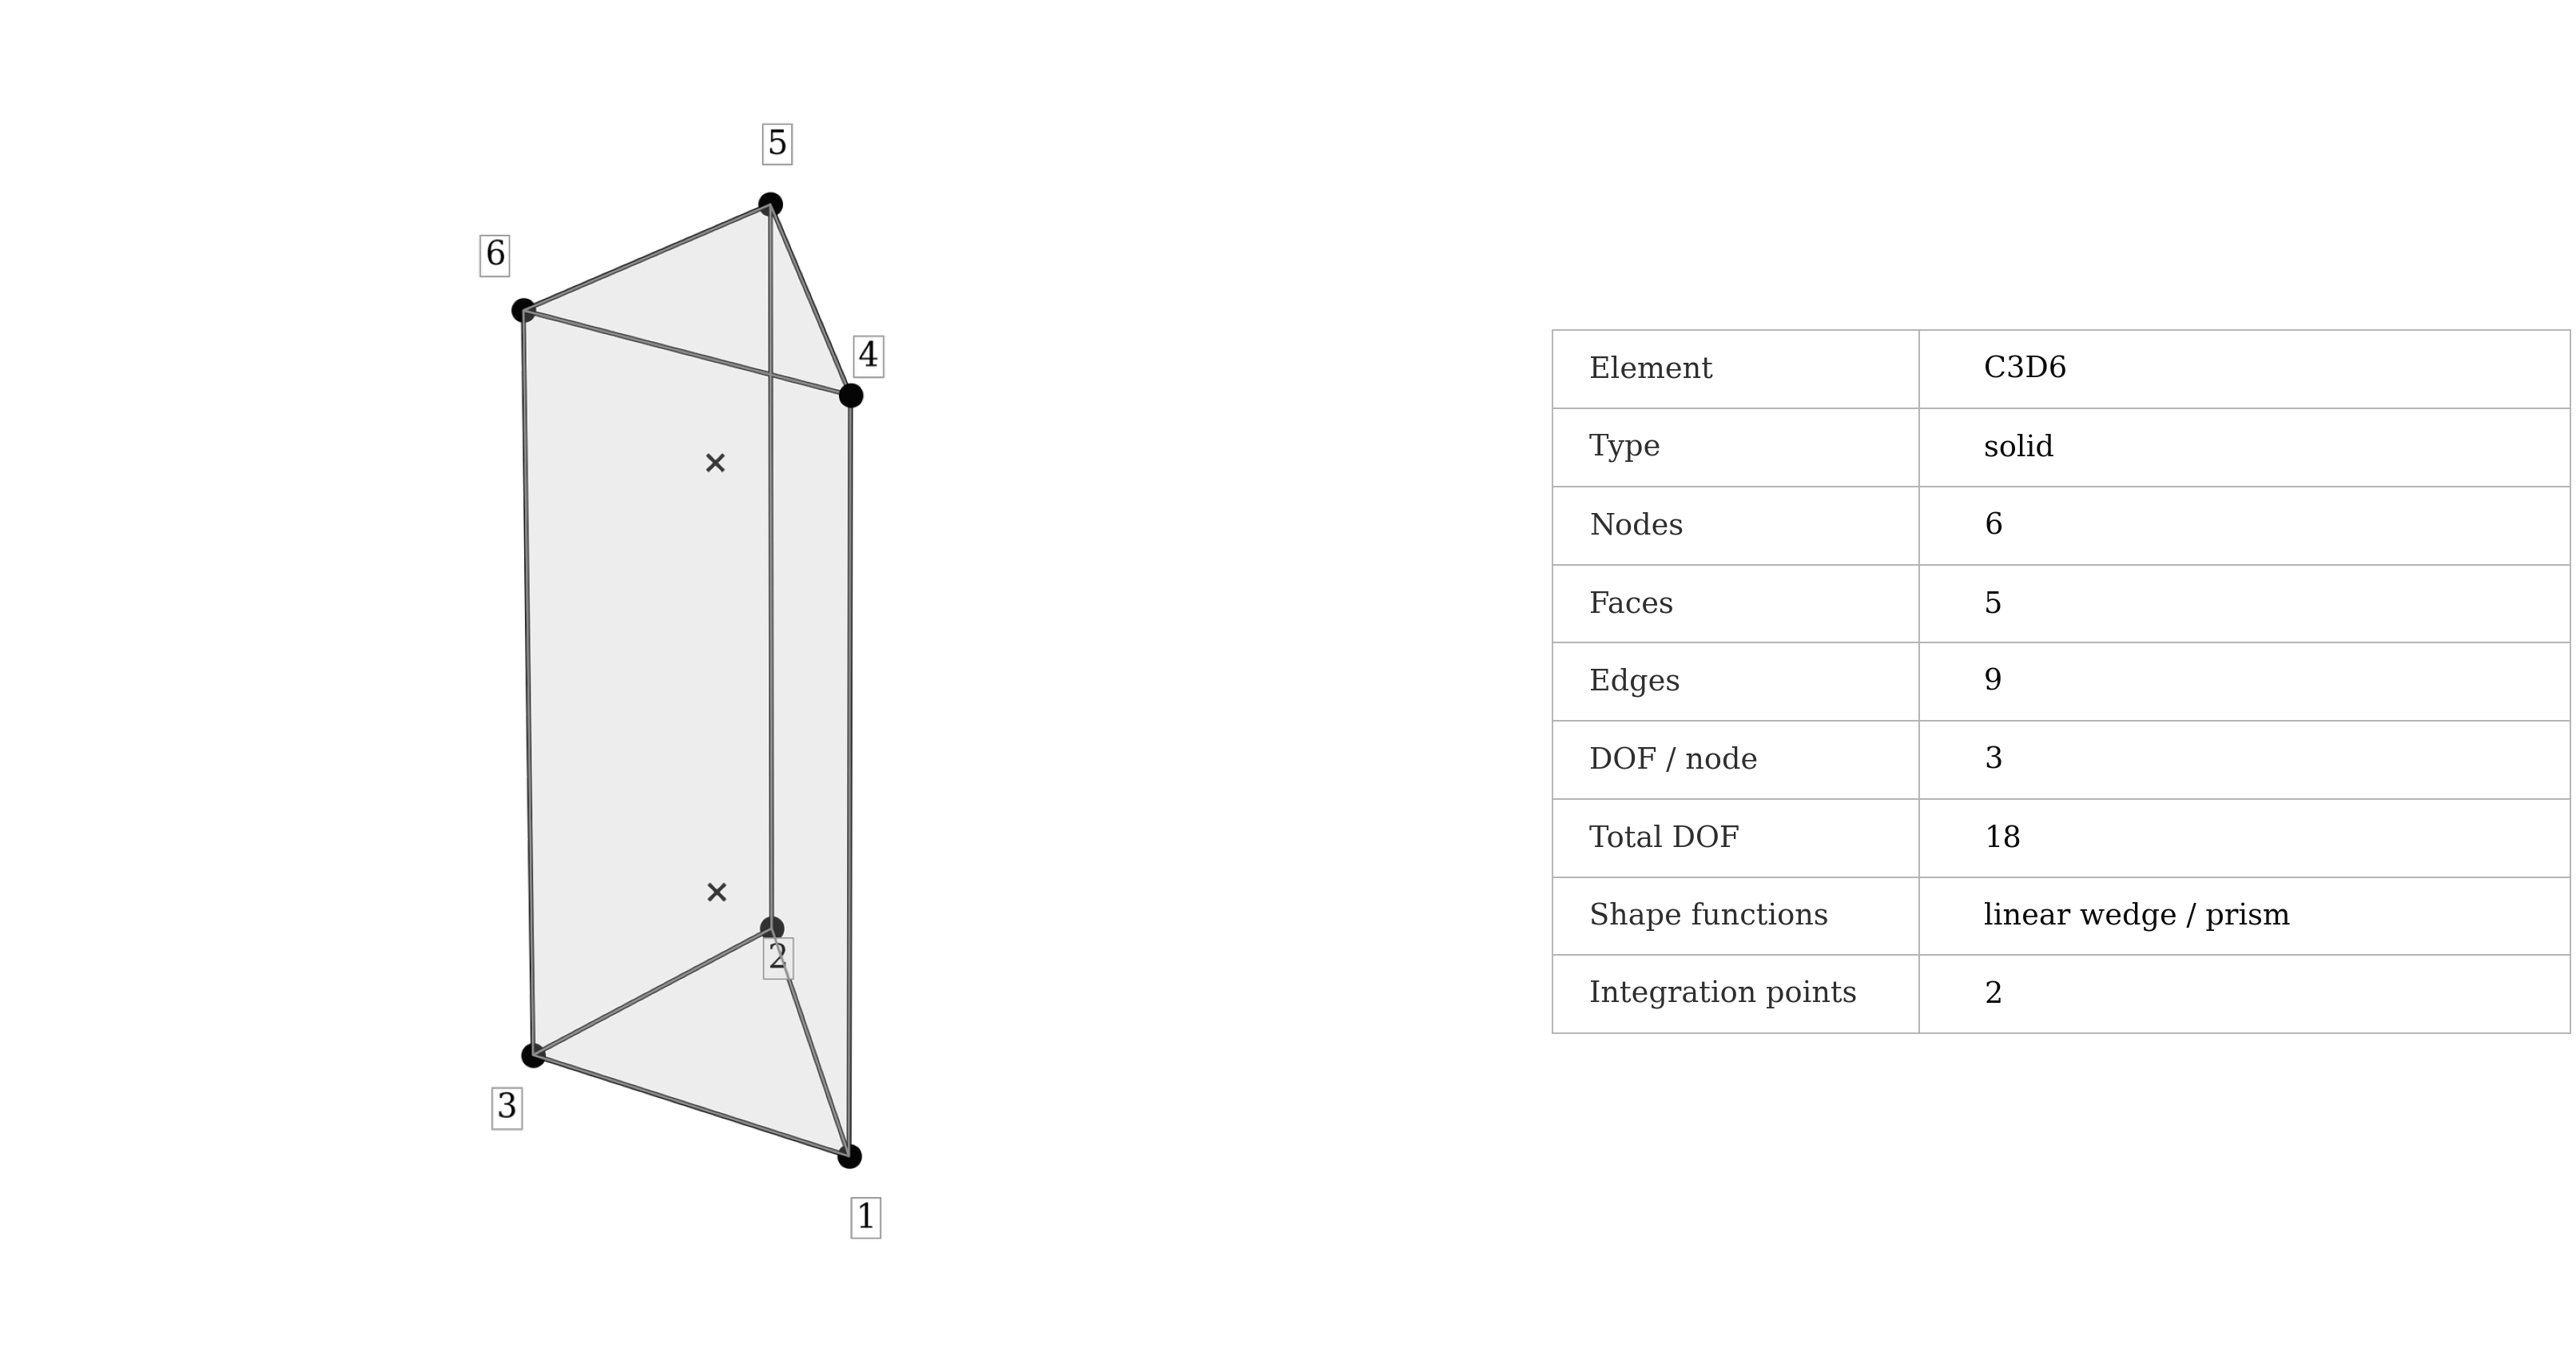
\includegraphics[width=0.78\linewidth]{pages/figures/element_schematics/c3d6_schematic.png}
    \caption{\val{C3D6} wedge element.}
\end{figure}

\begin{syntax}
*ELEMENT, TYPE=C3D6, ELSET=<set>
<id>, <n1>, <n2>, <n3>, <n4>, <n5>, <n6>
\end{syntax}

\val{C3D6} is a linear wedge or prism element. It combines triangular end faces with quadrilateral side faces and is particularly useful for swept meshes, extruded triangular surface meshes, layered regions, and transitions where a purely hexahedral topology is not possible.

A wedge mesh can align naturally with a dominant through-thickness or extrusion direction. This is useful in locally layered solids and prismatic regions because the element rows can follow the physical geometry more consistently than an unstructured tetrahedral mesh.

Like other low-order elements, \val{C3D6} has limited bending and gradient resolution. One or two linear wedges through the thickness of a bending-dominated region are rarely sufficient for accurate stress recovery. Refine in the direction of expected gradients and avoid collapsed triangular faces, excessive twisting between end faces, and highly skewed side faces.

Use \val{C3D6} when wedge topology is geometrically natural. If a quadratic swept mesh is available and higher accuracy is required, \val{C3D15} is the corresponding higher-order choice.

\clearpage
\section{\val{C3D8}: 8-node hexahedral solid}

\begin{figure}[H]
    \centering
    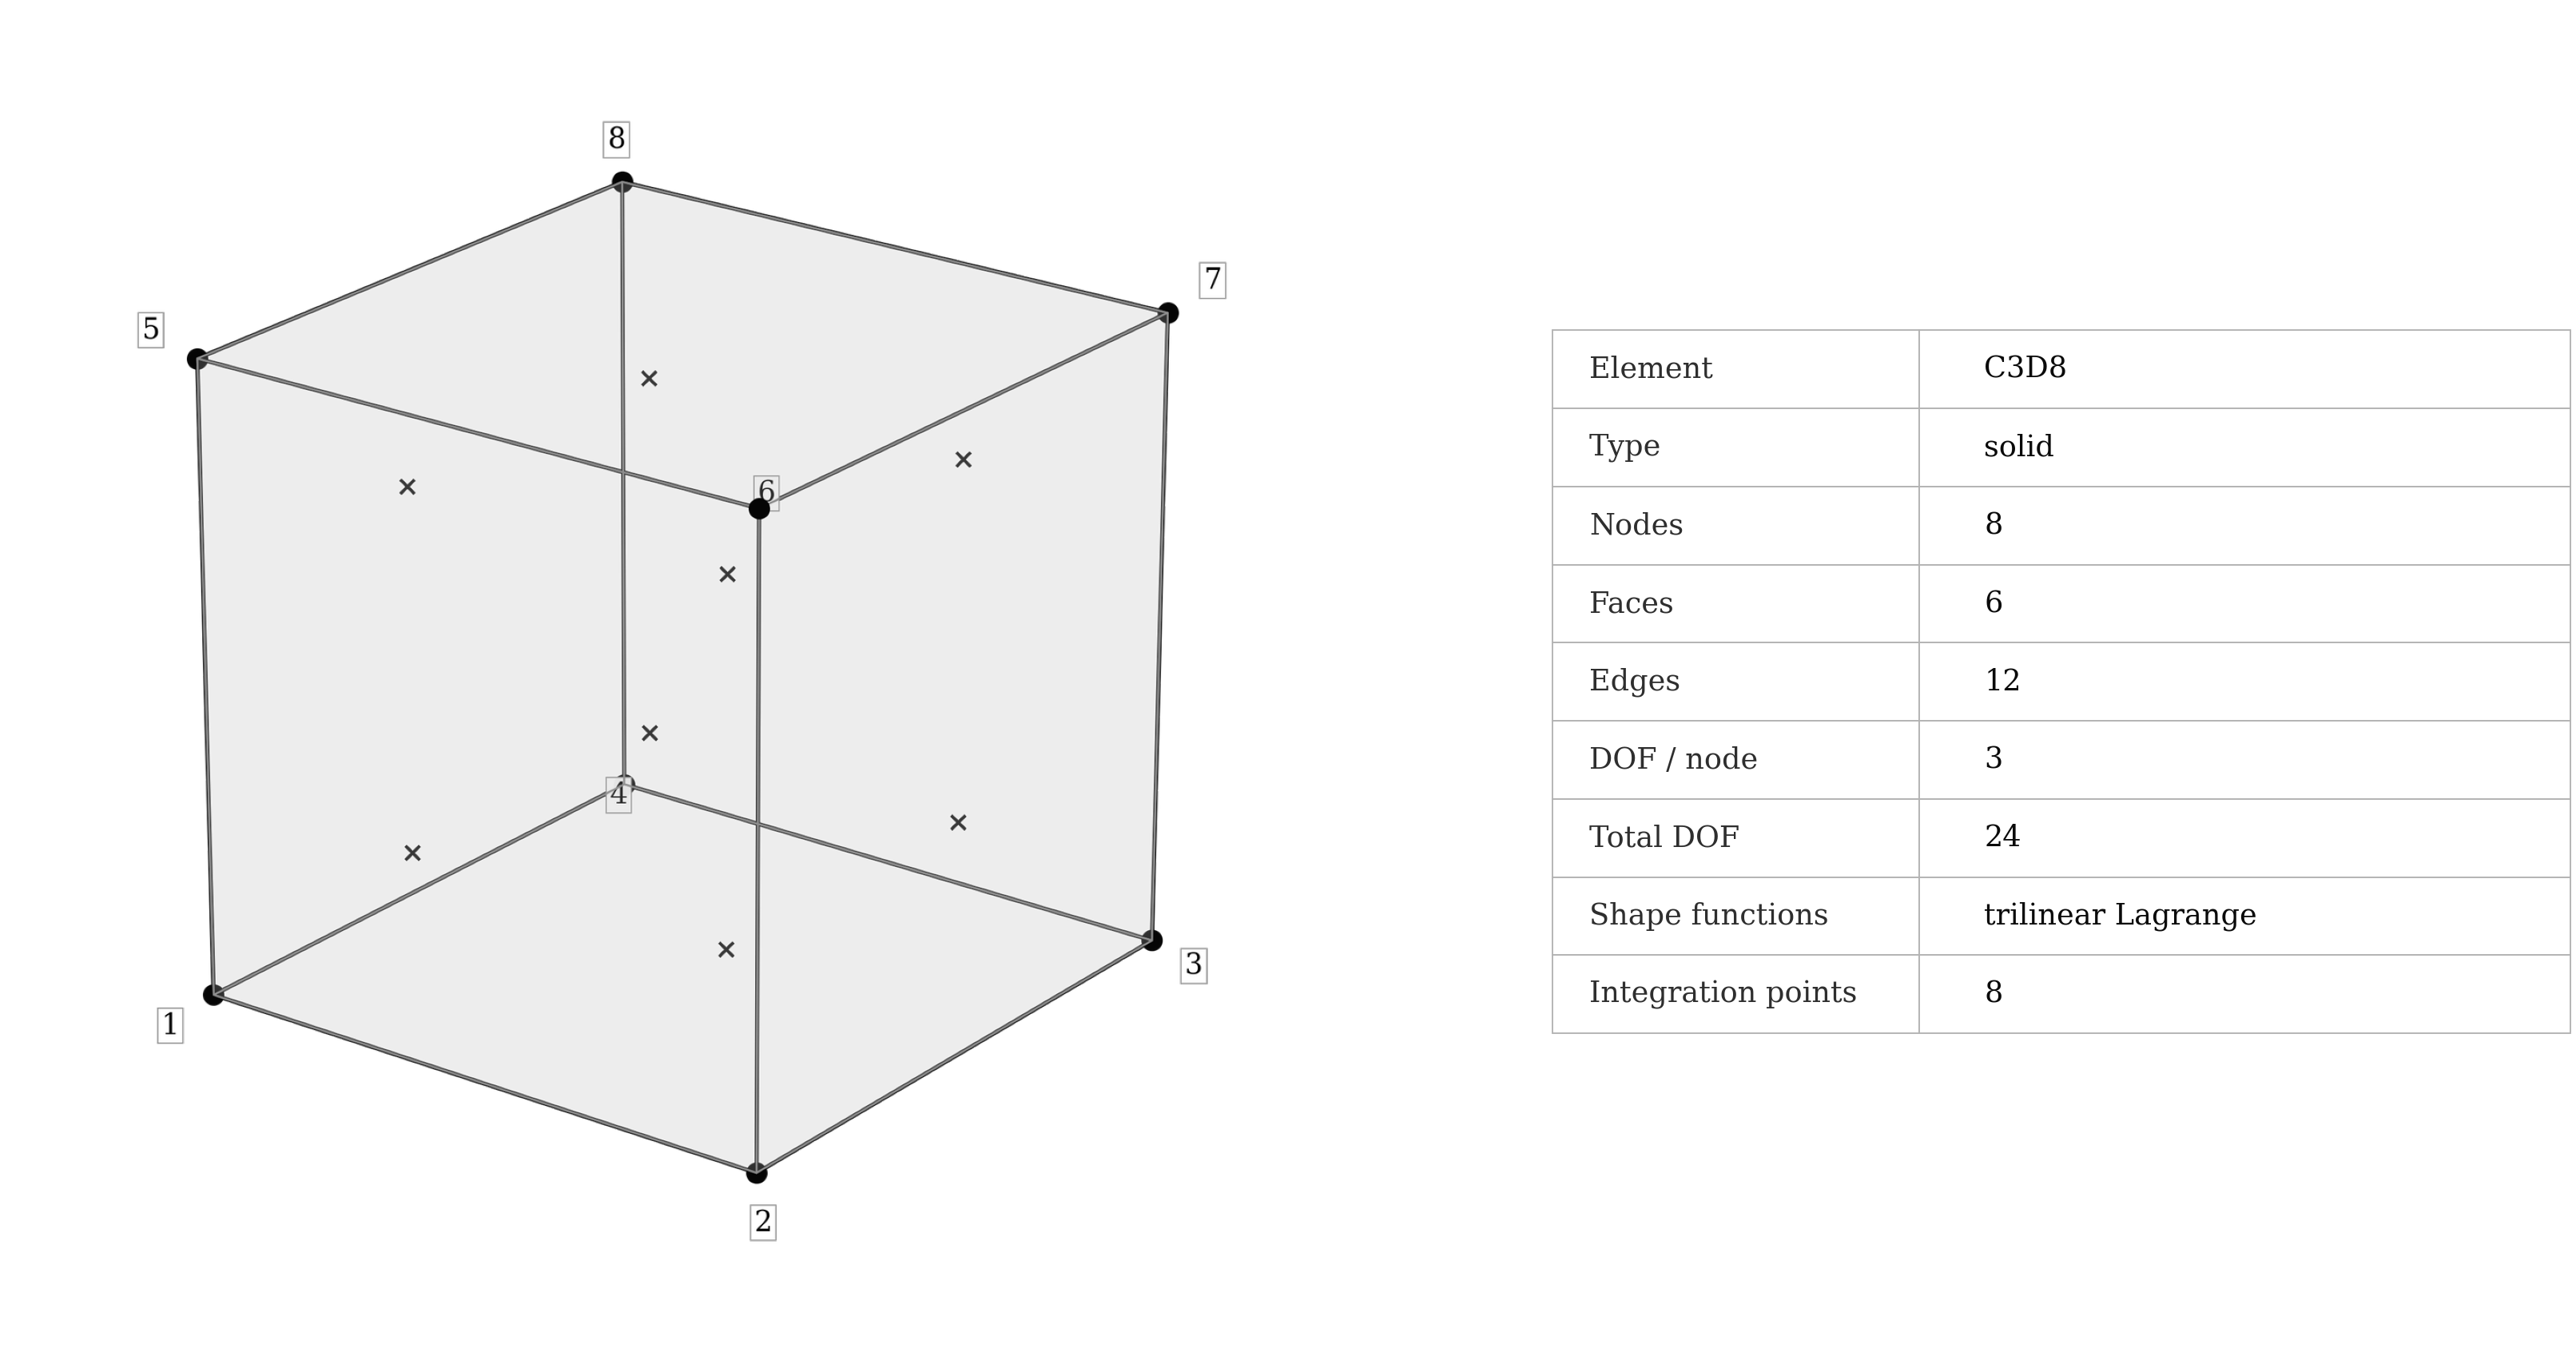
\includegraphics[width=0.82\linewidth]{pages/figures/element_schematics/c3d8_schematic.png}
    \caption{\val{C3D8} hexahedral solid element.}
\end{figure}

\begin{syntax}
*ELEMENT, TYPE=C3D8, ELSET=<set>
<id>, <n1>, <n2>, <n3>, <n4>, <n5>, <n6>, <n7>, <n8>
\end{syntax}

\val{C3D8} is the standard low-order hexahedral continuum element. It uses trilinear displacement interpolation and full integration. For regular block-like, swept, or layered meshes it is often an efficient general-purpose solid because element directions can follow geometry and material orientation naturally.

Hexahedral topology makes it easy to control the number of elements through thickness and along structural load paths. A good \val{C3D8} mesh is therefore attractive for plates modelled with solids, bonded layers, spars, ribs, extruded components, and regions where orthotropic material axes should follow the mesh.

The element remains low order. A coarse mesh can be too stiff in bending, and straight element edges only approximate curved boundaries. Use several elements through thickness when solid bending stresses are important and refine curved or stress-critical geometry sufficiently.

Warping, skew, negative Jacobians, and extreme aspect ratios can destroy the advantages of the hexahedral topology. A clean quadratic tetrahedral mesh can be better than a badly distorted hexahedral mesh. Inspect mesh quality instead of selecting \val{C3D8} solely because hexahedra are usually preferred.

\clearpage
\section{\val{C3D8R}: reduced-integration 8-node hexahedral solid}

\begin{figure}[H]
    \centering
    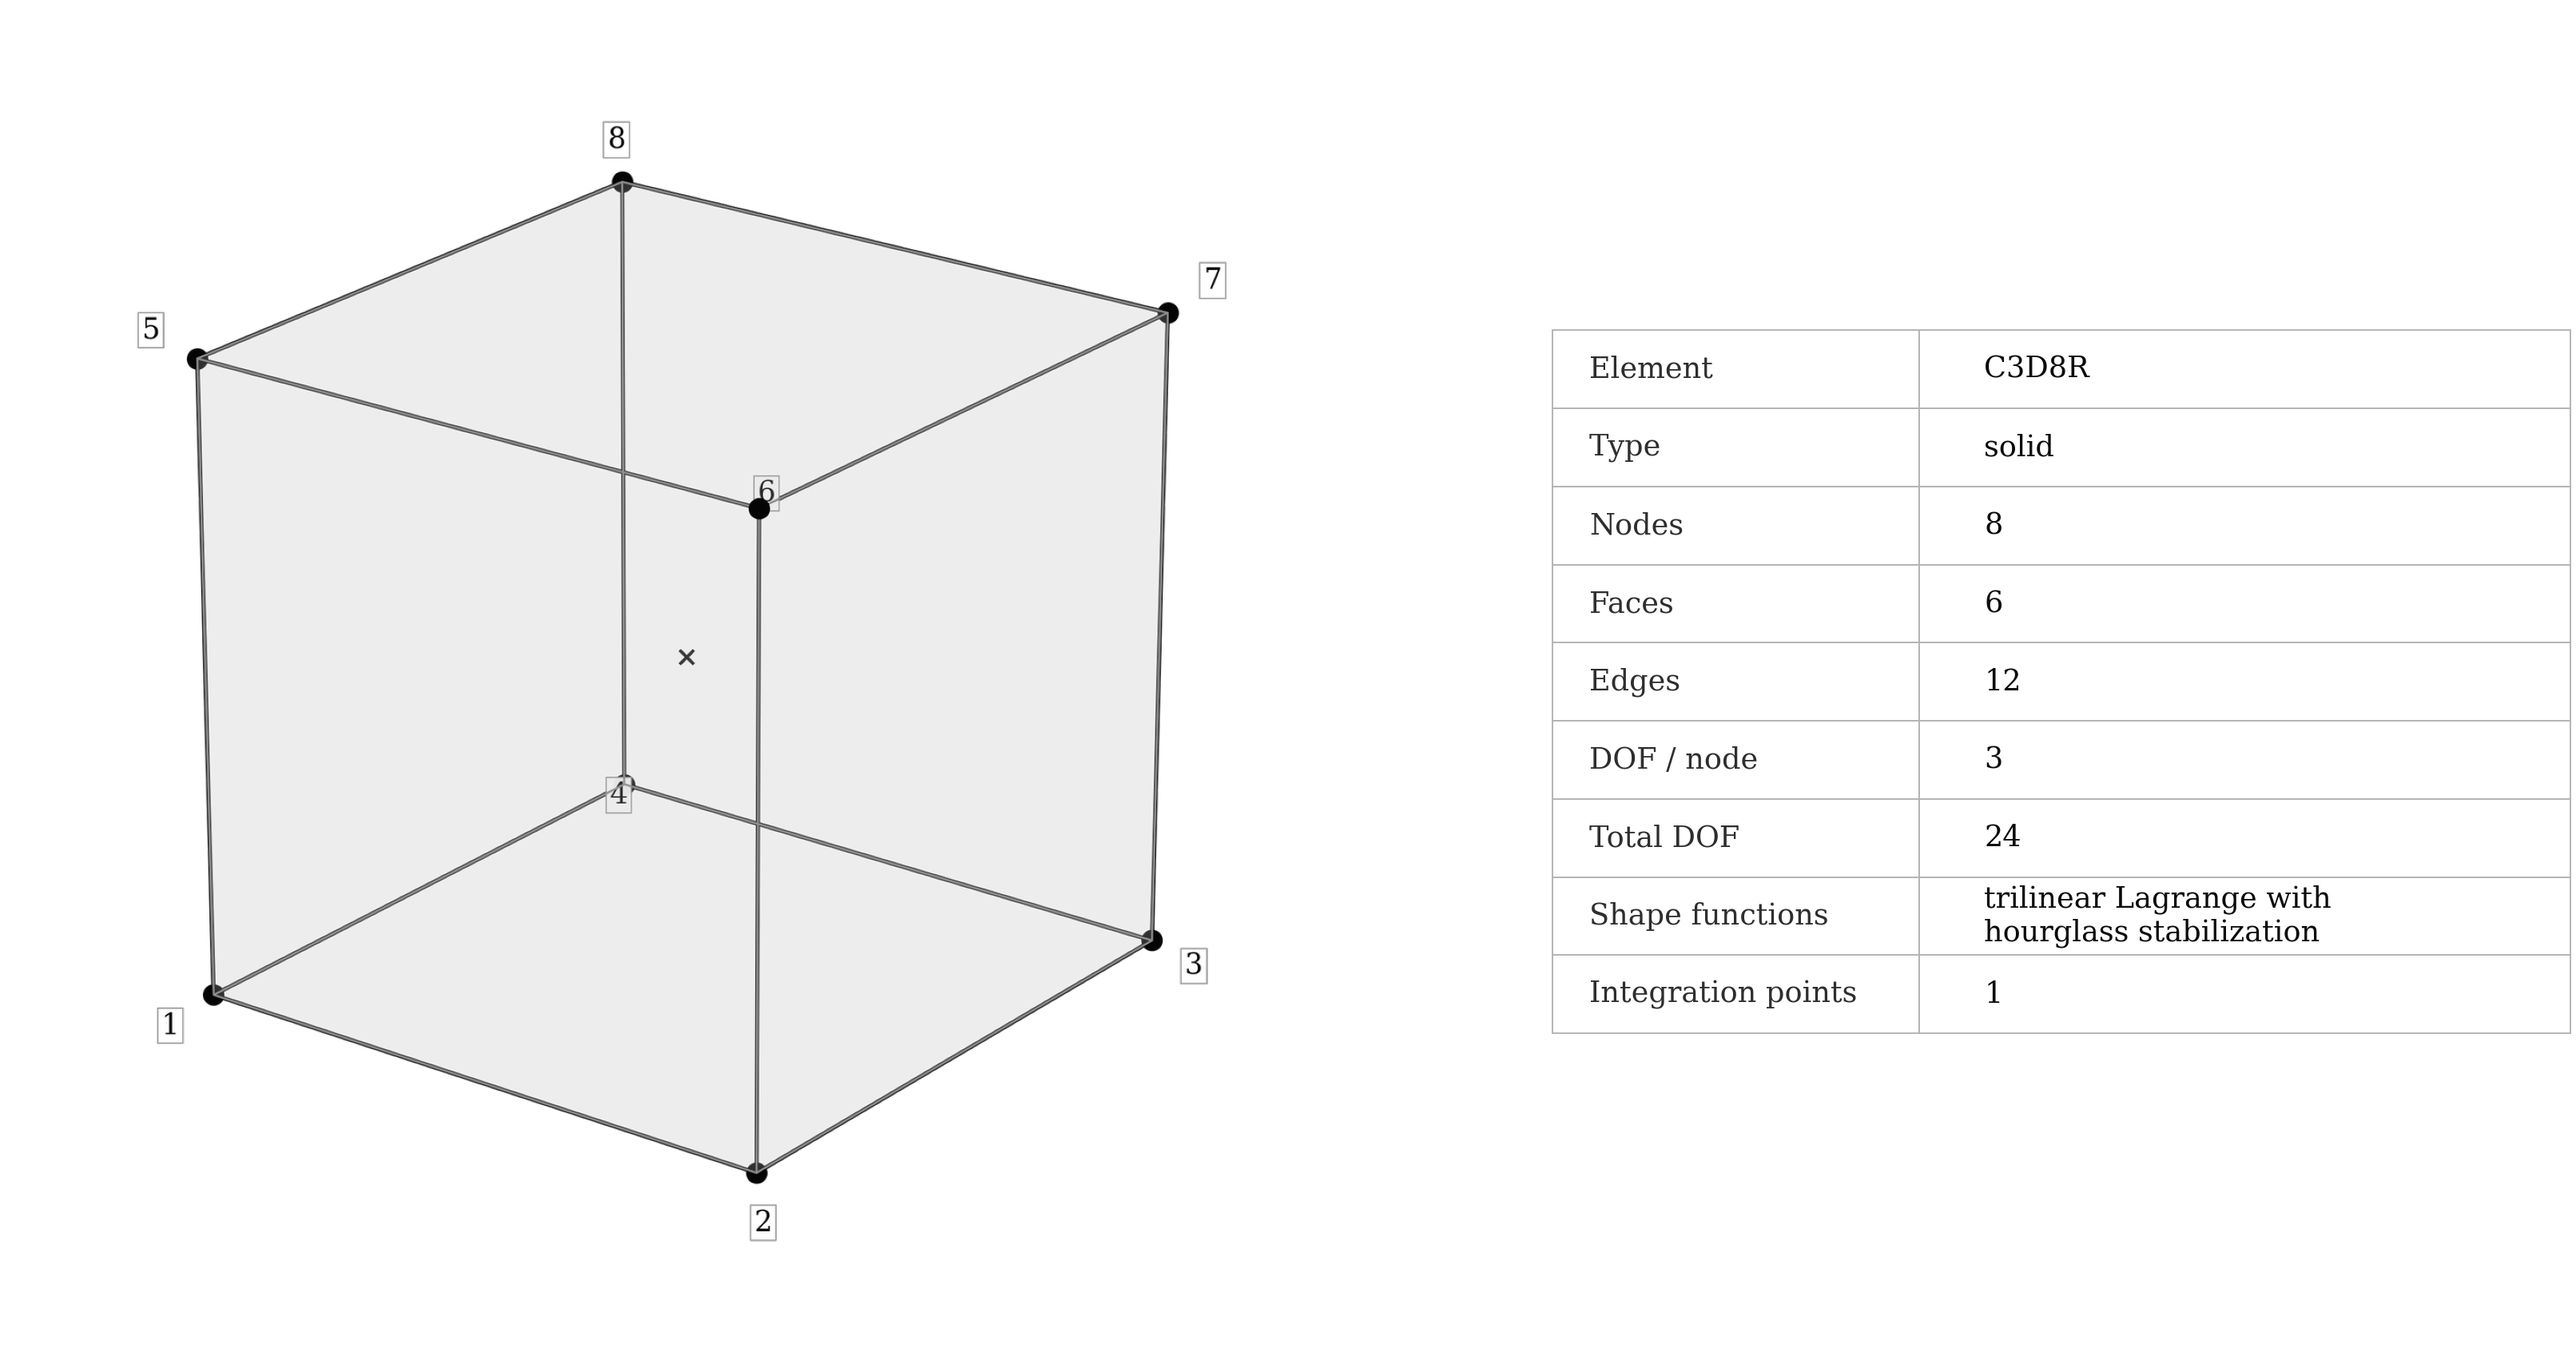
\includegraphics[width=0.82\linewidth]{pages/figures/element_schematics/c3d8r_schematic.png}
    \caption{\val{C3D8R} reduced-integration hexahedral solid element.}
\end{figure}

\begin{syntax}
*ELEMENT, TYPE=C3D8R, ELSET=<set>
<id>, <n1>, <n2>, <n3>, <n4>, <n5>, <n6>, <n7>, <n8>
\end{syntax}

\val{C3D8R} uses the same eight-node topology as \val{C3D8} but evaluates the continuum contribution with one integration point at the element centre. Reduced integration lowers assembly cost and avoids some of the excessive stiffness that a fully integrated low-order hexahedron can exhibit in bending-dominated states.

One-point integration also introduces zero-energy hourglass deformation modes. FEMaster therefore adds hourglass stabilization. The primitive scalar hourglass patterns are based on the four non-affine modes
\[
\gamma_1=s\,t,\qquad
\gamma_2=t\,r,\qquad
\gamma_3=r\,s,\qquad
\gamma_4=r\,s\,t.
\]
These modes are projected so that affine displacement fields are not penalized. The stabilization scale is based on the element reference volume, the reference geometry gradients, and an effective shear stiffness derived from the constitutive tangent.

The practical consequence is that \val{C3D8R} should be judged not only by Newton convergence but also by its deformation pattern and stabilization sensitivity. A model may converge while still exhibiting nonphysical hourglass deformation if the mesh is too coarse or badly distorted. Compare suspicious regions with \val{C3D8}, refine the mesh, and inspect whether the response changes strongly when the hourglass-sensitive deformation is resolved geometrically.

For severe finite rotations or highly distorted elements, reduced-integration stabilization deserves particular scrutiny. Use \val{C3D8R} deliberately when its lower locking tendency or cost is beneficial, rather than as an automatic replacement for \val{C3D8}.

\clearpage
\section{\val{C3D10}: 10-node quadratic tetrahedral solid}

\begin{figure}[H]
    \centering
    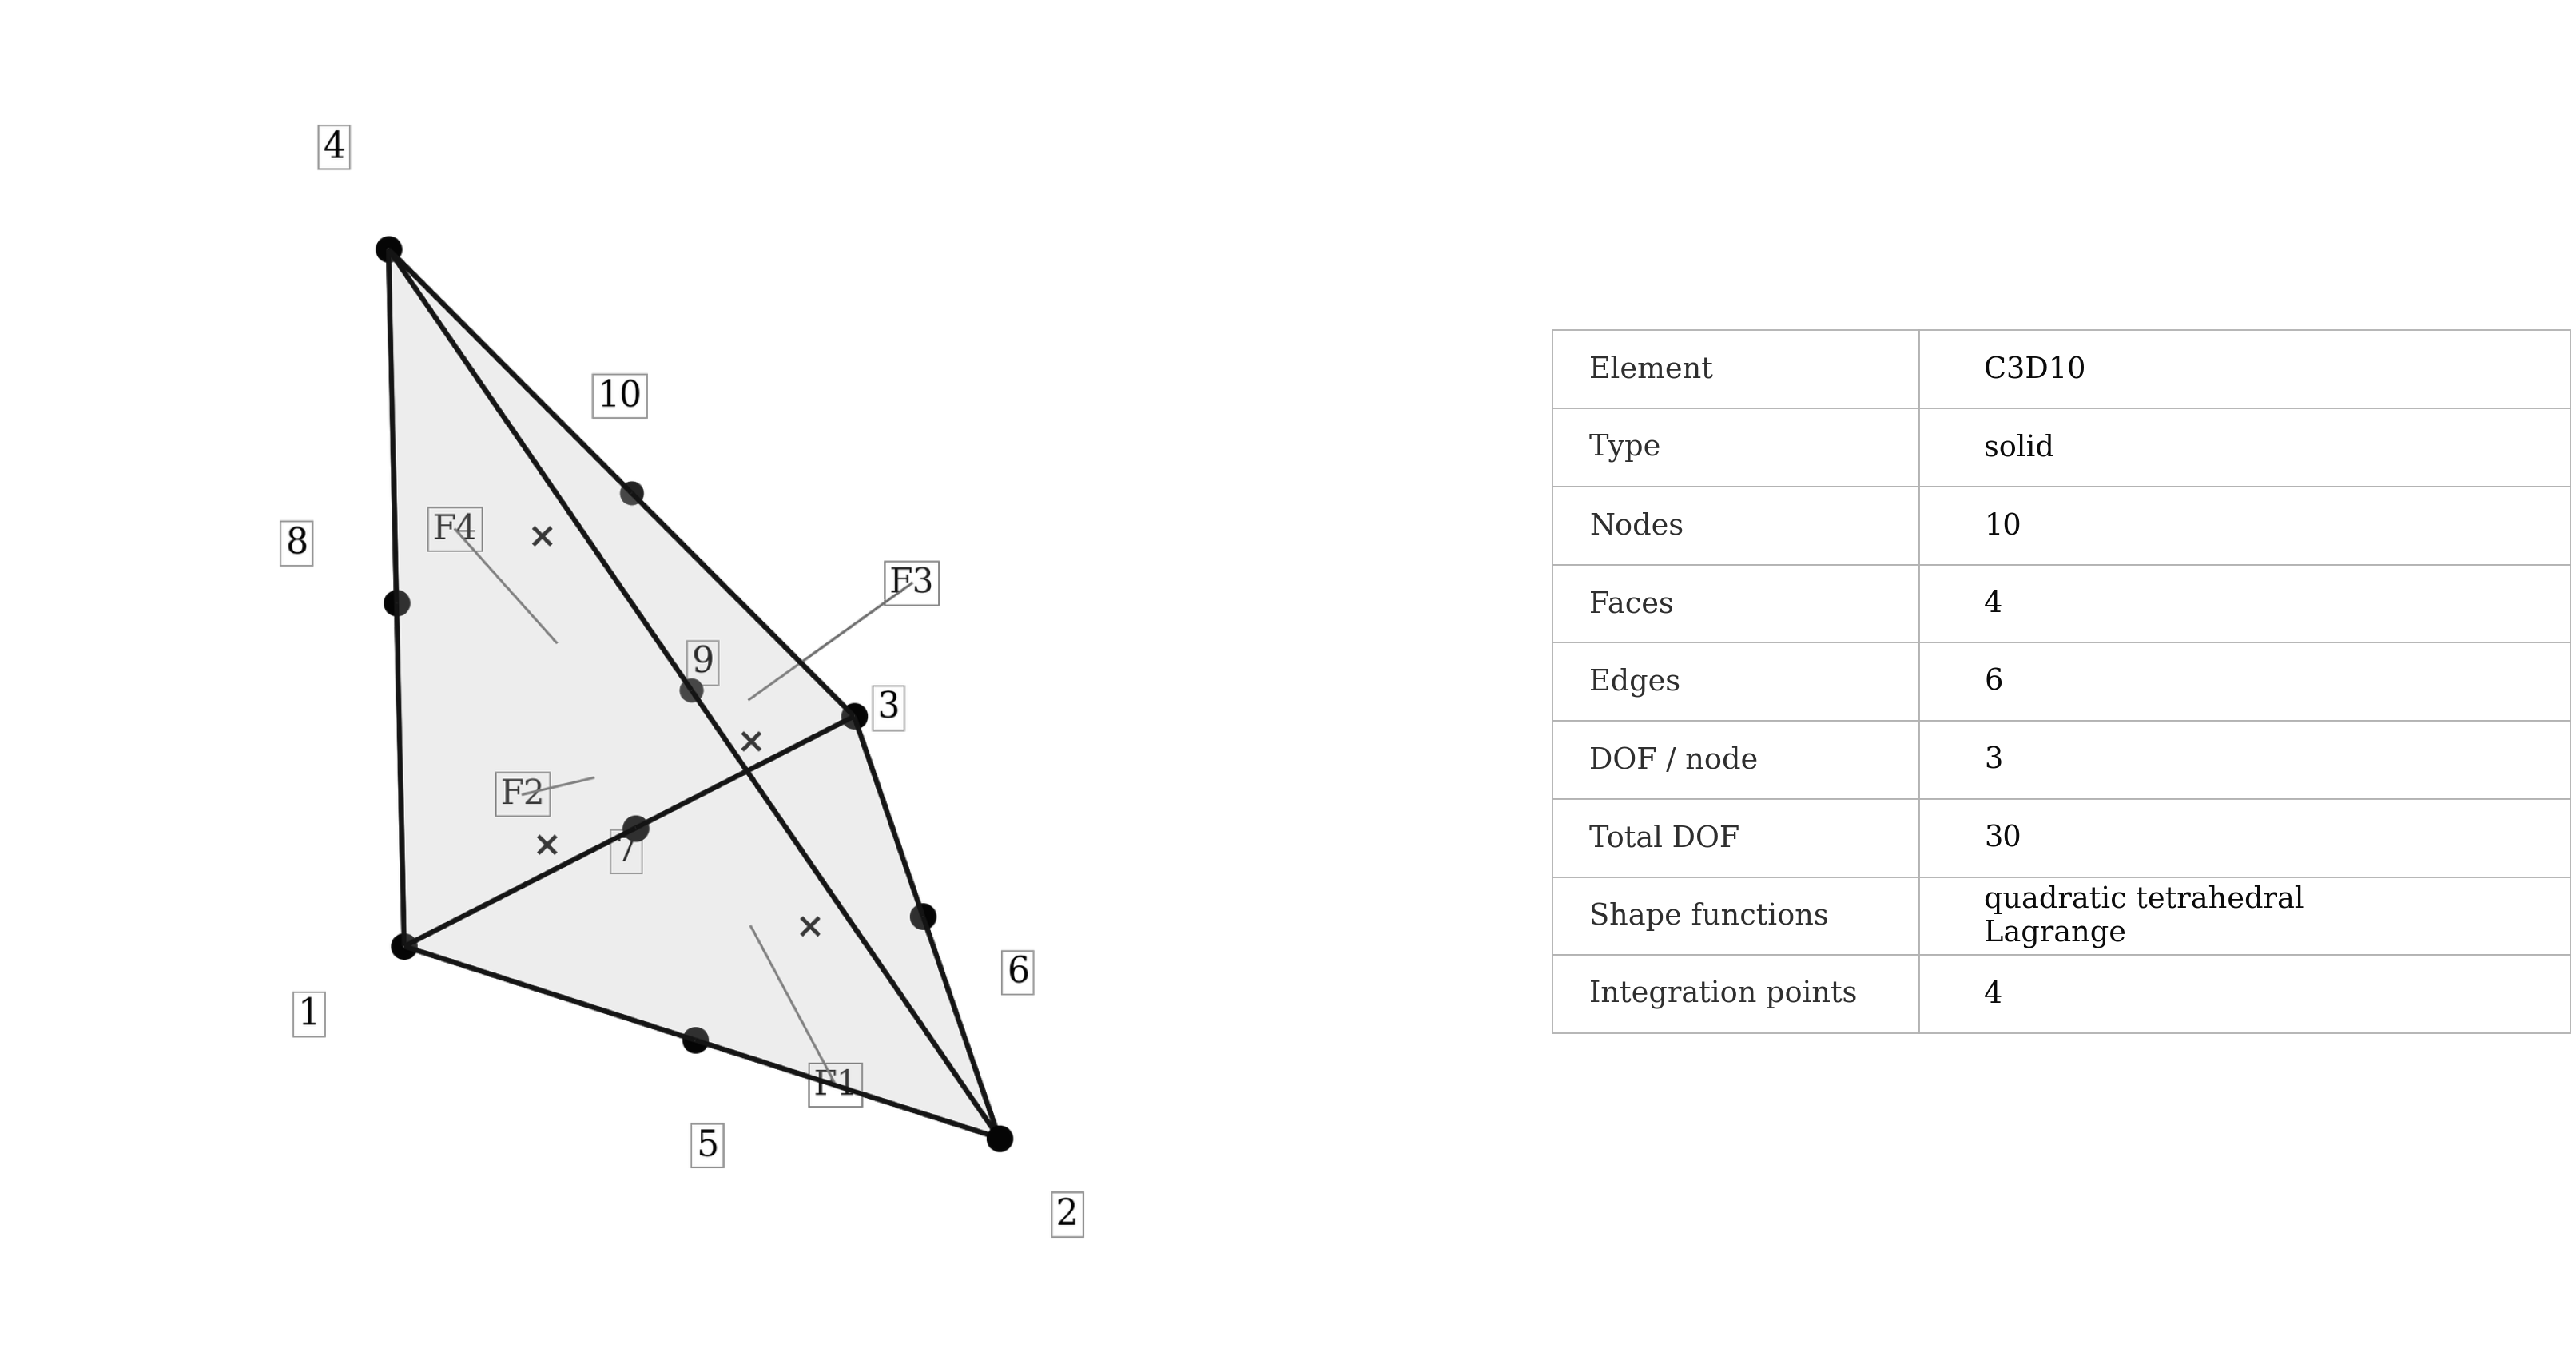
\includegraphics[width=0.80\linewidth]{pages/figures/element_schematics/c3d10_schematic.png}
    \caption{\val{C3D10} quadratic tetrahedral element.}
\end{figure}

\begin{syntax}
*ELEMENT, TYPE=C3D10, ELSET=<set>
<id>, <n1>, <n2>, <n3>, <n4>, <n5>, <n6>, <n7>, <n8>, <n9>, <n10>
\end{syntax}

\val{C3D10} is the quadratic tetrahedral solid. Six midside nodes augment the four corner nodes and allow quadratic displacement interpolation. Compared with \val{C3D4}, the element can represent curved deformation, bending, and stress gradients far more efficiently.

For automatic tetrahedral meshing, \val{C3D10} is generally the preferred engineering stress element. It keeps the geometric flexibility of tetrahedra while reducing the excessive stiffness and piecewise-constant strain behaviour associated with linear tetrahedra.

The quadratic geometry mapping also represents curved boundaries more accurately when midside nodes follow the CAD geometry. Those midside positions must remain sensible: badly displaced midside nodes can create a distorted mapping even if the corner tetrahedron appears acceptable.

The element costs more per cell than \val{C3D4}, but substantially fewer cells may be required for comparable displacement and stress accuracy. Refinement is still required near singularities, sharp re-entrant corners, and concentrated loads where no polynomial element can make a mathematical singularity disappear.

\clearpage
\section{\val{C3D15}: 15-node quadratic wedge solid}

\begin{figure}[H]
    \centering
    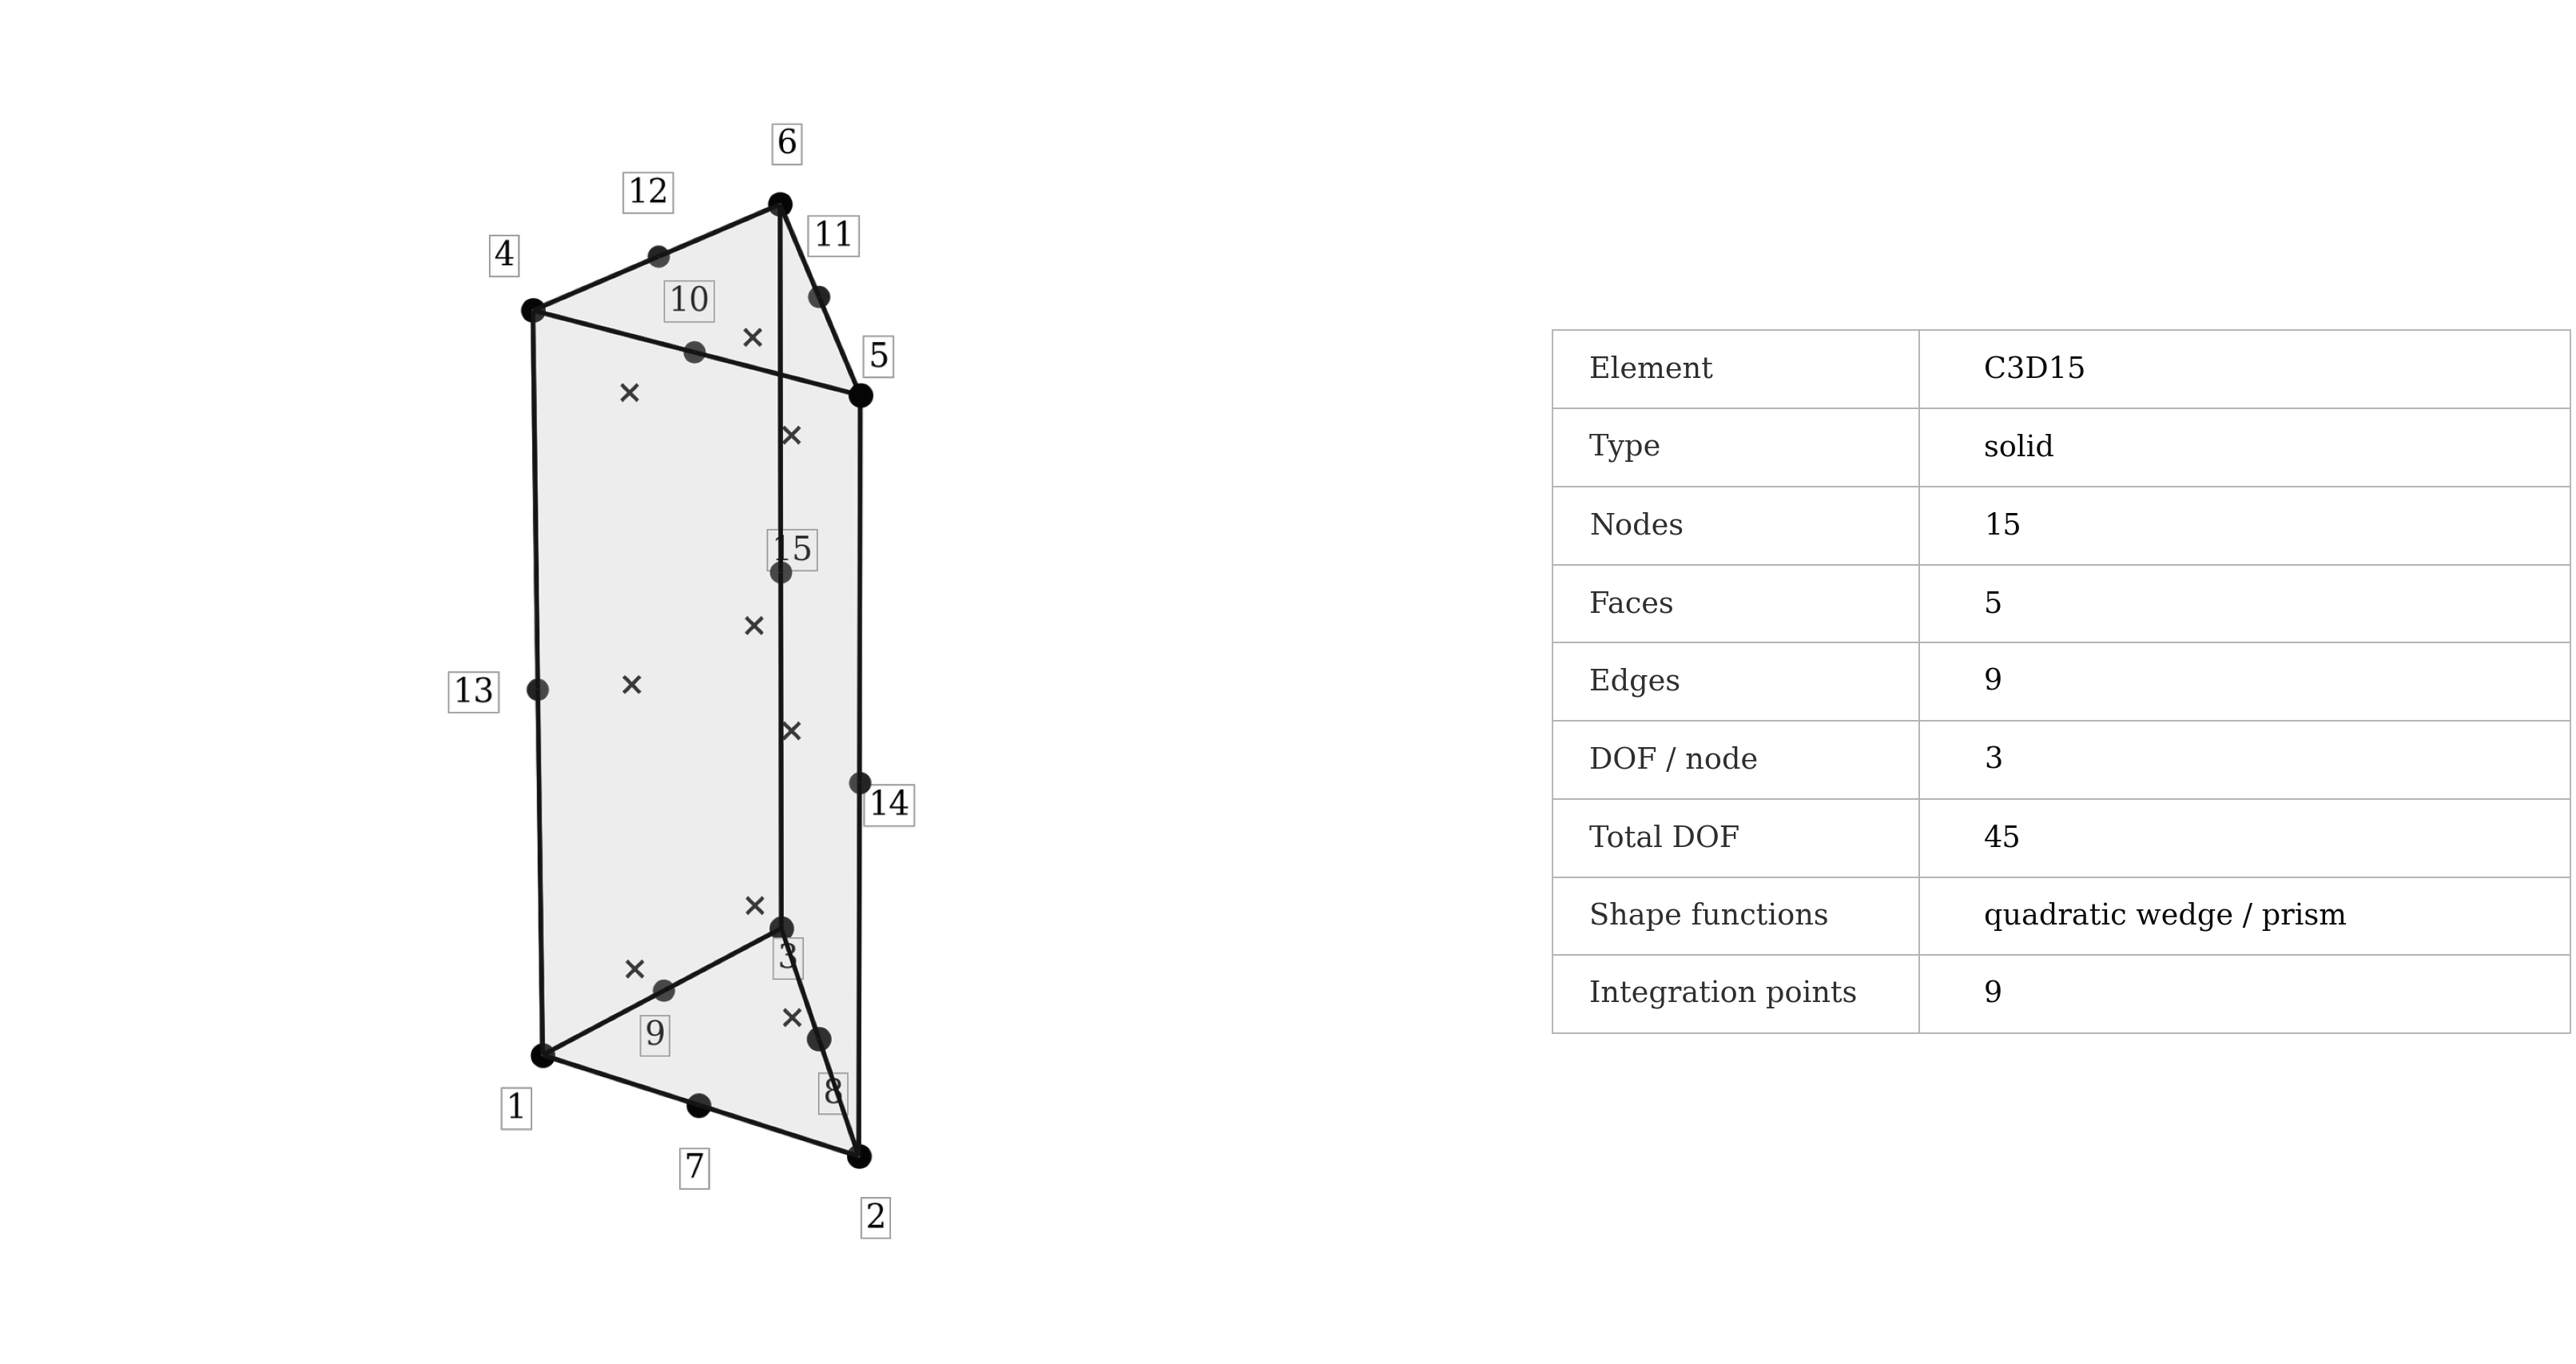
\includegraphics[width=0.80\linewidth]{pages/figures/element_schematics/c3d15_schematic.png}
    \caption{\val{C3D15} quadratic wedge element.}
\end{figure}

\begin{syntax}
*ELEMENT, TYPE=C3D15, ELSET=<set>
<id>, <n1>, ..., <n15>
\end{syntax}

\val{C3D15} is the quadratic counterpart of the six-node wedge. It adds midside nodes and can represent curvature, bending, and through-thickness gradients more effectively than \val{C3D6}. It is particularly useful in higher-order swept meshes and in prismatic regions created by extruding a quadratic triangular surface mesh.

The element is attractive when wedge topology is natural but low-order through-thickness behaviour is insufficient. Curved swept solids, local layered regions, and transition zones can often be represented with fewer elements than would be needed with \val{C3D6}.

Higher-order mapping increases sensitivity to midside-node placement. The triangular end faces should remain well shaped, the side faces should not twist excessively, and midside nodes should follow the intended geometry smoothly. A high-order wedge with a poor mapping is not automatically more accurate than a clean low-order mesh.

Use \val{C3D15} for deliberate quadratic wedge meshes. If the geometry supports a structured quadratic hexahedral mesh, \val{C3D20} may provide a more regular discretization; for fully unstructured complex geometry, \val{C3D10} is often easier to generate robustly.

\clearpage
\section{\val{C3D20}: 20-node quadratic hexahedral solid}

\begin{figure}[H]
    \centering
    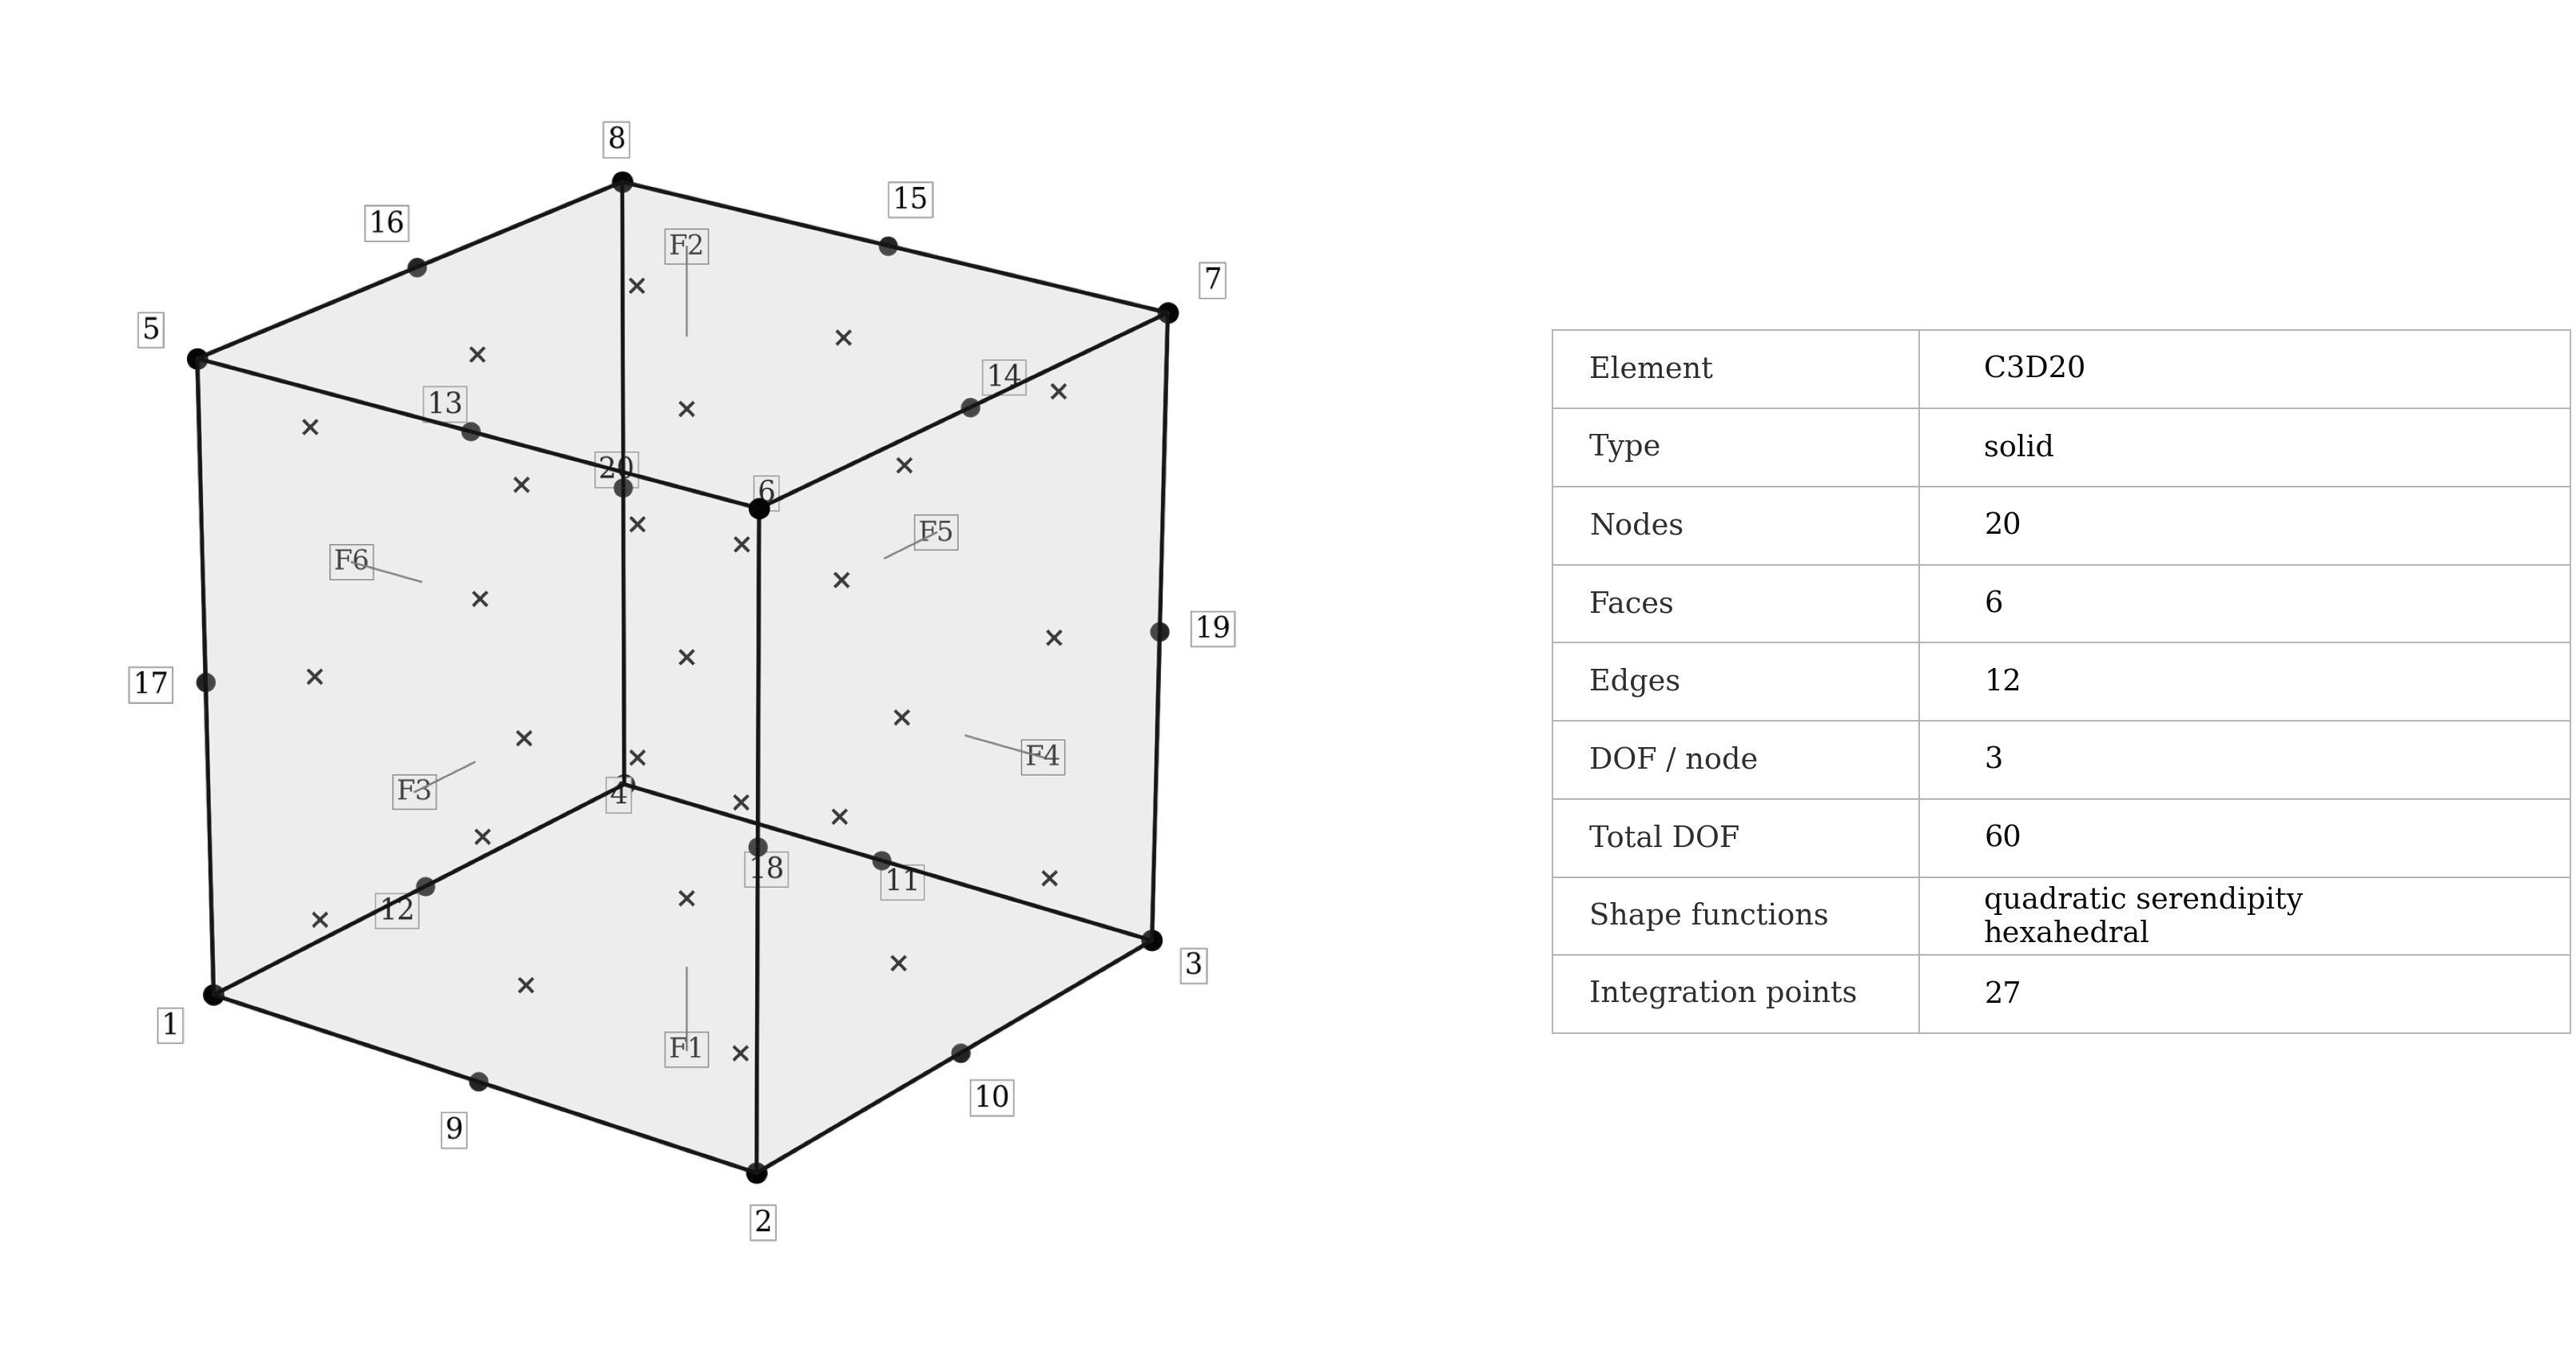
\includegraphics[width=0.82\linewidth]{pages/figures/element_schematics/c3d20_schematic.png}
    \caption{\val{C3D20} quadratic hexahedral element.}
\end{figure}

\begin{syntax}
*ELEMENT, TYPE=C3D20, ELSET=<set>
<id>, <n1>, ..., <n20>
\end{syntax}

\val{C3D20} is the full-integration quadratic hexahedral solid. The eight corner nodes are supplemented by twelve midside nodes, giving the element substantially better bending and stress-gradient representation than \val{C3D8}. Curved geometry can also be represented more accurately when midside nodes follow the physical boundary.

For smooth structural fields and high-quality structured meshes, \val{C3D20} is one of the most accurate solid choices available in FEMaster. It is well suited to curved blocks, swept volumes, thick structural regions, and stress-recovery problems where a high-order hexahedral mesh can be generated reliably.

The main costs are larger element matrices and stricter geometric quality requirements. Distortion of a quadratic mapping can be more harmful than distortion of a linear one because the midside nodes participate directly in the geometry interpolation. Check Jacobian quality and avoid arbitrary movement of midside nodes.

Choose \val{C3D20} when accuracy and mesh quality justify the additional cost. For models dominated by linear global stiffness where a fine regular mesh already exists, \val{C3D8} may remain more economical.

\clearpage
\section{\val{C3D20R}: 20-node reduced-integration hexahedral solid}

\begin{figure}[H]
    \centering
    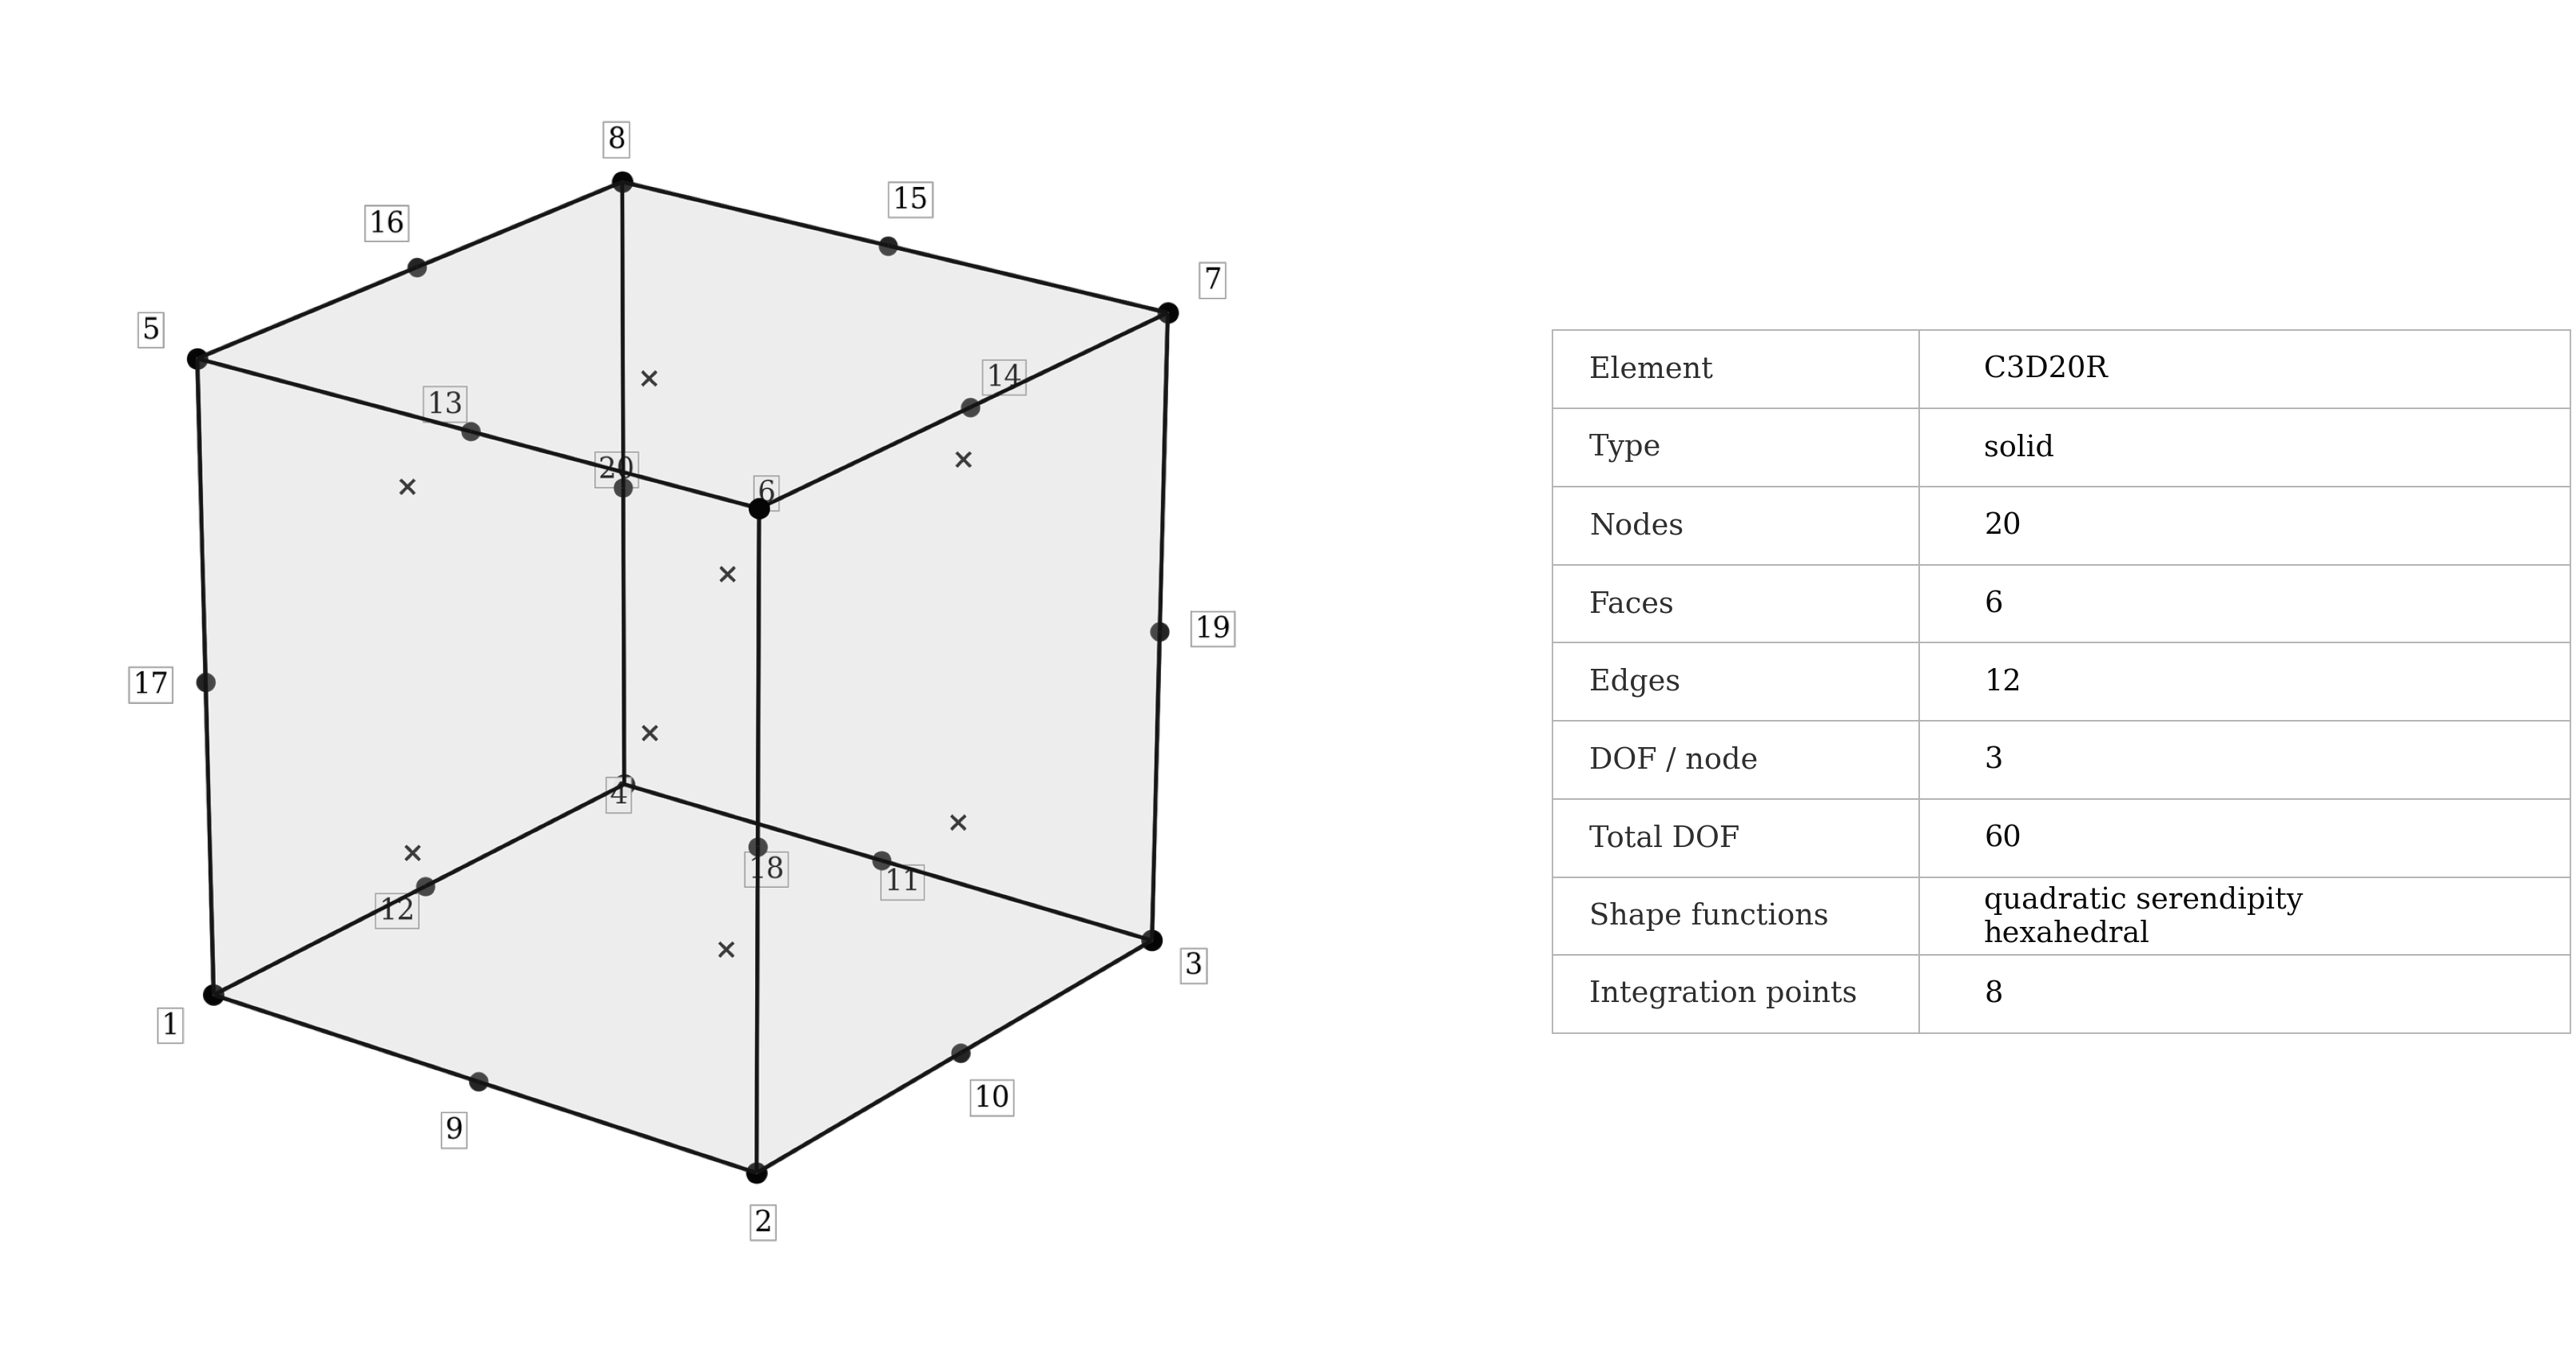
\includegraphics[width=0.82\linewidth]{pages/figures/element_schematics/c3d20r_schematic.png}
    \caption{\val{C3D20R} reduced-integration quadratic hexahedral element.}
\end{figure}

\begin{syntax}
*ELEMENT, TYPE=C3D20R, ELSET=<set>
<id>, <n1>, ..., <n20>
\end{syntax}

\val{C3D20R} uses the same twenty-node topology and quadratic interpolation as \val{C3D20}, but the stiffness contribution is evaluated with reduced integration. The reduced rule lowers cost and can improve behaviour in states where full integration introduces excessive constraint or stiffness.

Reduced integration changes the numerical character of the element; it is not merely a faster switch. The model should therefore be checked for nonphysical low-energy deformation modes and sensitivity to mesh distortion. Deformed shapes, reaction balance, strain-energy distribution, and comparison with \val{C3D20} provide useful diagnostics.

The formulation is most attractive when a good quadratic hexahedral mesh is already available and the analyst has a reason to prefer reduced integration. For routine work where robustness is more important than the reduced rule, \val{C3D20} is the more conservative comparison element.

\section{Shell elements}

Shell elements reduce a three-dimensional thin structure to a two-dimensional midsurface with membrane, bending, and transverse-shear behaviour. They are appropriate when thickness is small relative to the in-plane dimensions and the main quantities of interest are surface displacements, membrane forces, bending moments, transverse shear resultants, and top/bottom shell stresses rather than detailed three-dimensional through-thickness stress fields.

Shell quality depends strongly on surface mesh quality, normal consistency, aspect ratio, element warping, and thickness definition. The shell normal determines the top/bottom convention and affects pressure direction and result signs. Curved shell models should therefore be checked visually for normal consistency before interpreting bending results.

\begin{warningbox}[Recommended shell family]
The native shell elements \val{S3}, \val{S4}, \val{MITC4}, \val{S6}, \val{S8}, and \val{MITC8} are retained for legacy decks, verification, and comparison. New production shell models should normally use the finite-rotation family \val{MITC3FRT}, \val{MITC4FRT}, \val{MITC6FRT}, or \val{MITC8FRT}. The supported Abaqus shell labels are translated to this FRT family automatically.
\end{warningbox}

\clearpage
\section{\val{S3}: legacy 3-node triangular shell}

\begin{figure}[H]
    \centering
    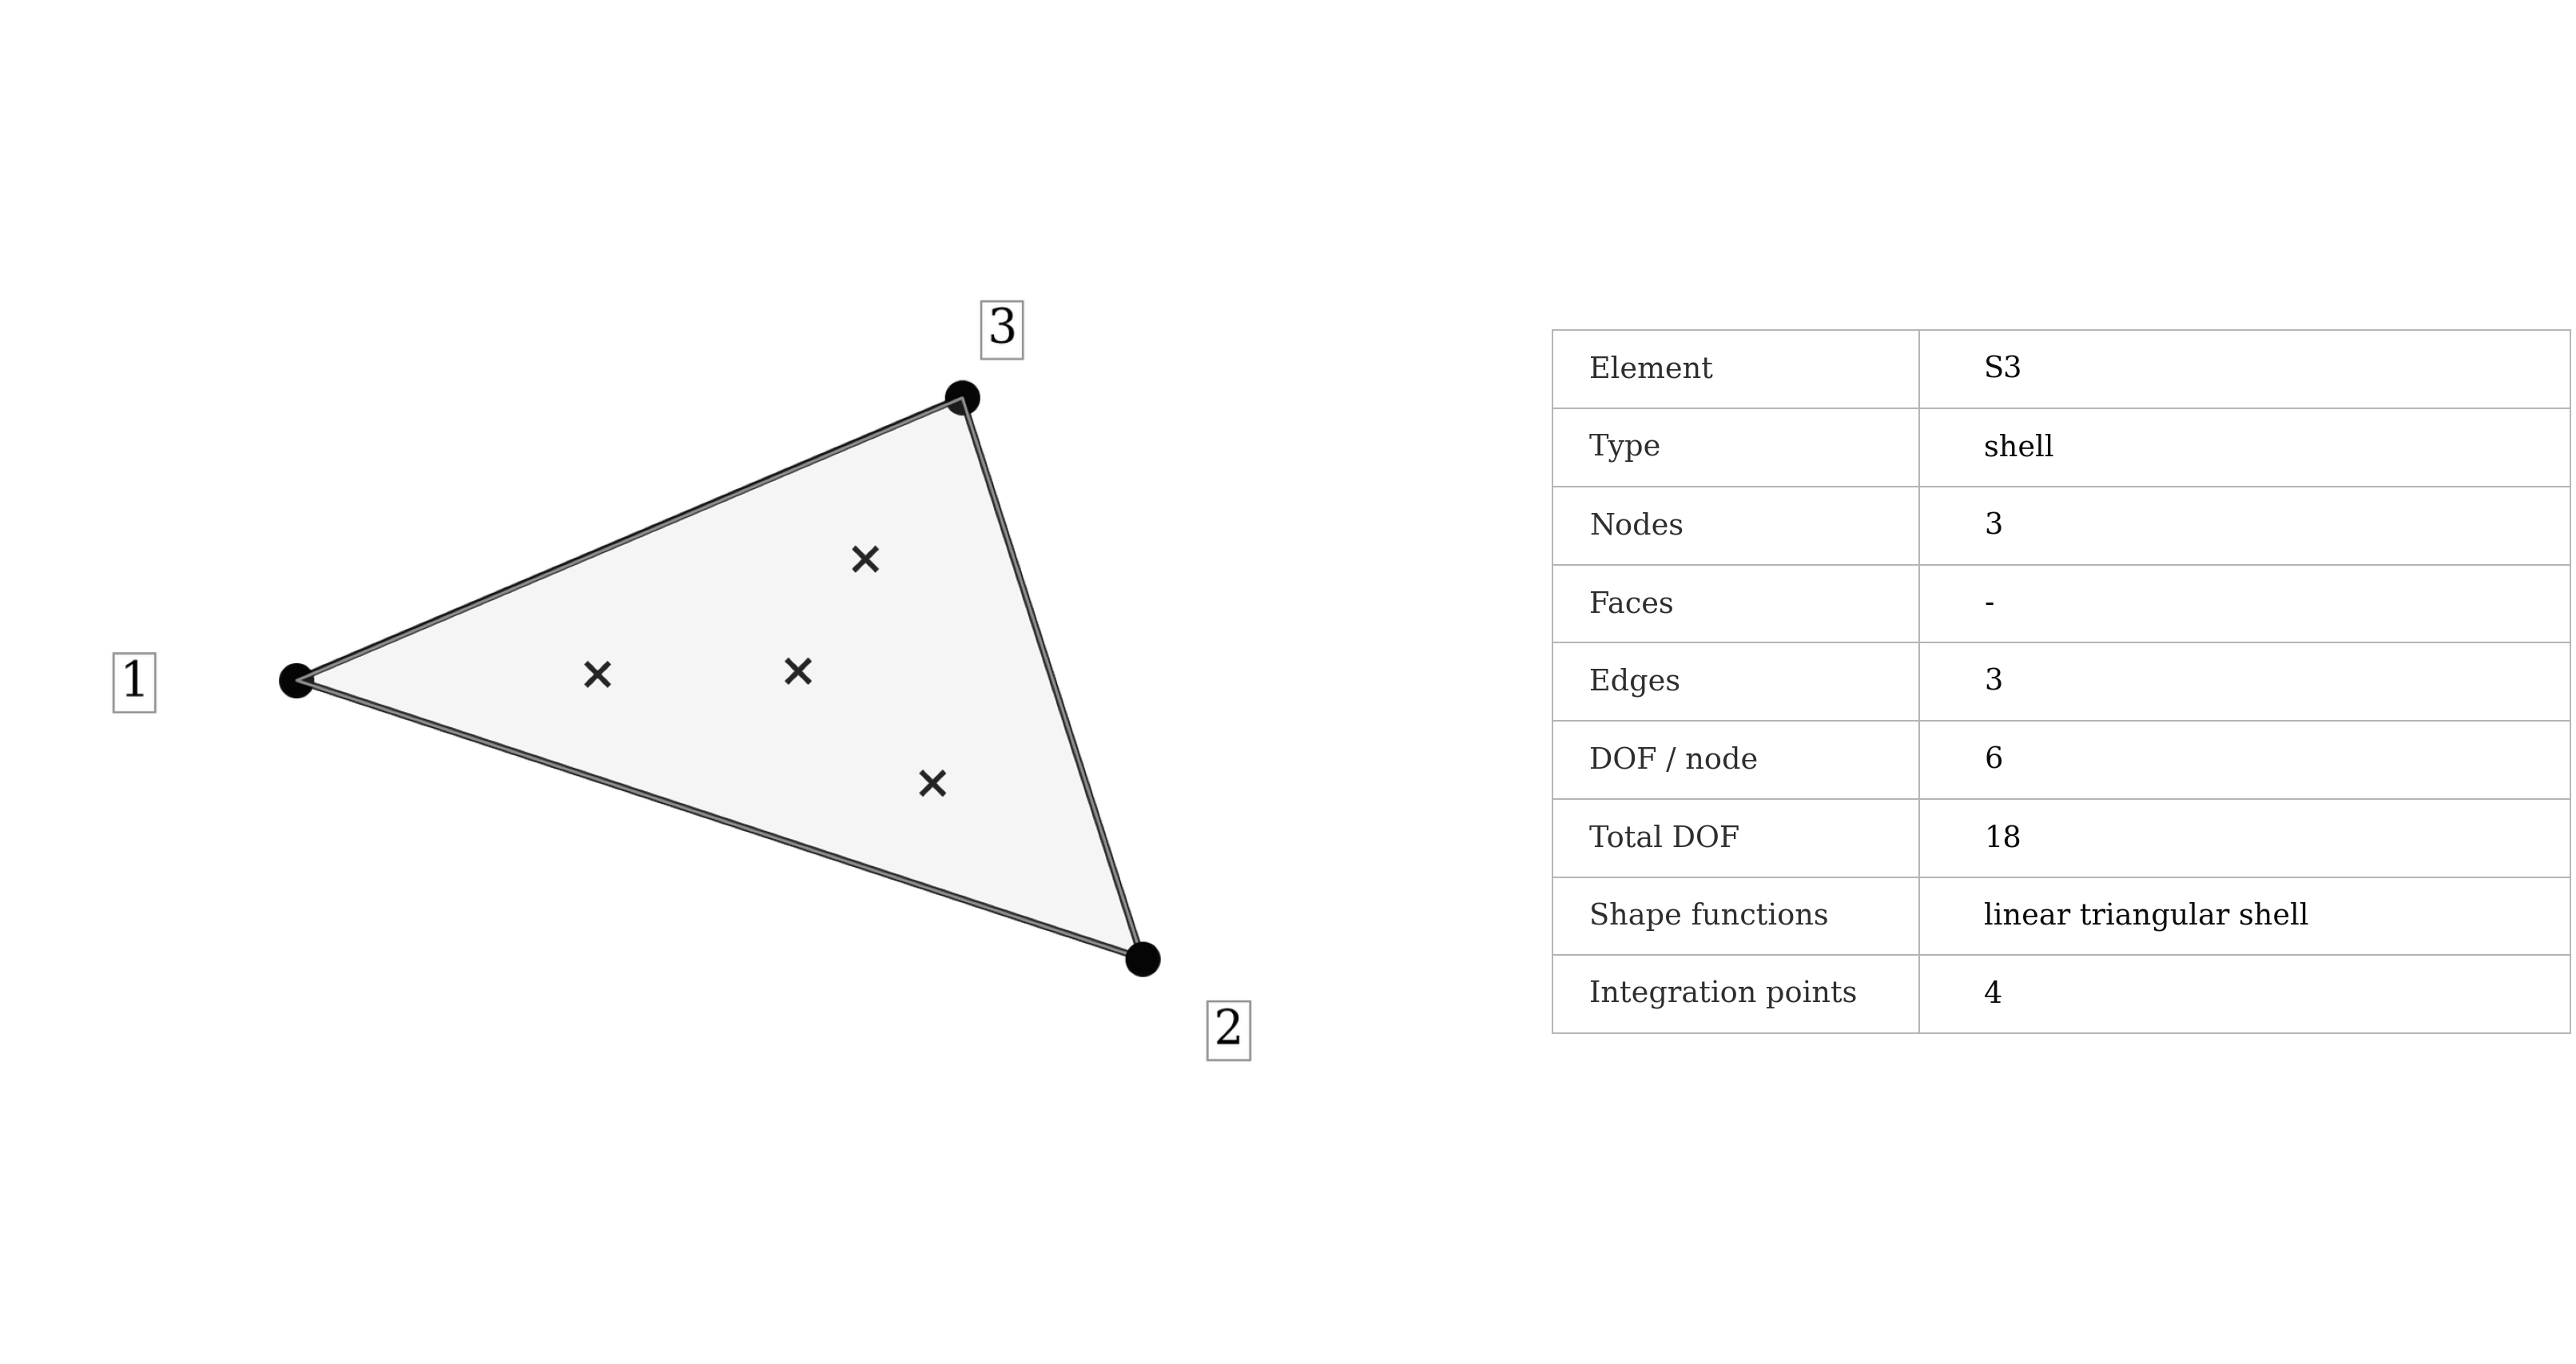
\includegraphics[width=0.76\linewidth]{pages/figures/element_schematics/s3_schematic.png}
    \caption{\val{S3} triangular shell topology.}
\end{figure}

\begin{syntax}
*ELEMENT, TYPE=S3, ELSET=<set>
<id>, <n1>, <n2>, <n3>
\end{syntax}

Native \val{S3} is the legacy three-node triangular shell. Triangular topology is useful for filling irregular surface meshes and transition regions, but a three-node triangle provides only low-order interpolation and typically needs a finer mesh than a good quadrilateral discretization for smooth bending fields.

The element remains accepted so older FEMaster decks continue to run and so legacy formulations can be compared with newer shells. For new work, use \val{MITC3FRT} instead. This recommendation is especially strong for geometrically nonlinear analyses and for models where finite rotations are expected.

Triangular shell meshes should avoid extremely acute angles, abrupt size changes, and inconsistent normal orientation. A dense mesh of poor triangles can still give inferior bending behaviour compared with a smaller set of well-shaped elements.

\clearpage
\section{\val{MITC3FRT}: finite-rotation 3-node shell}

\begin{figure}[H]
    \centering
    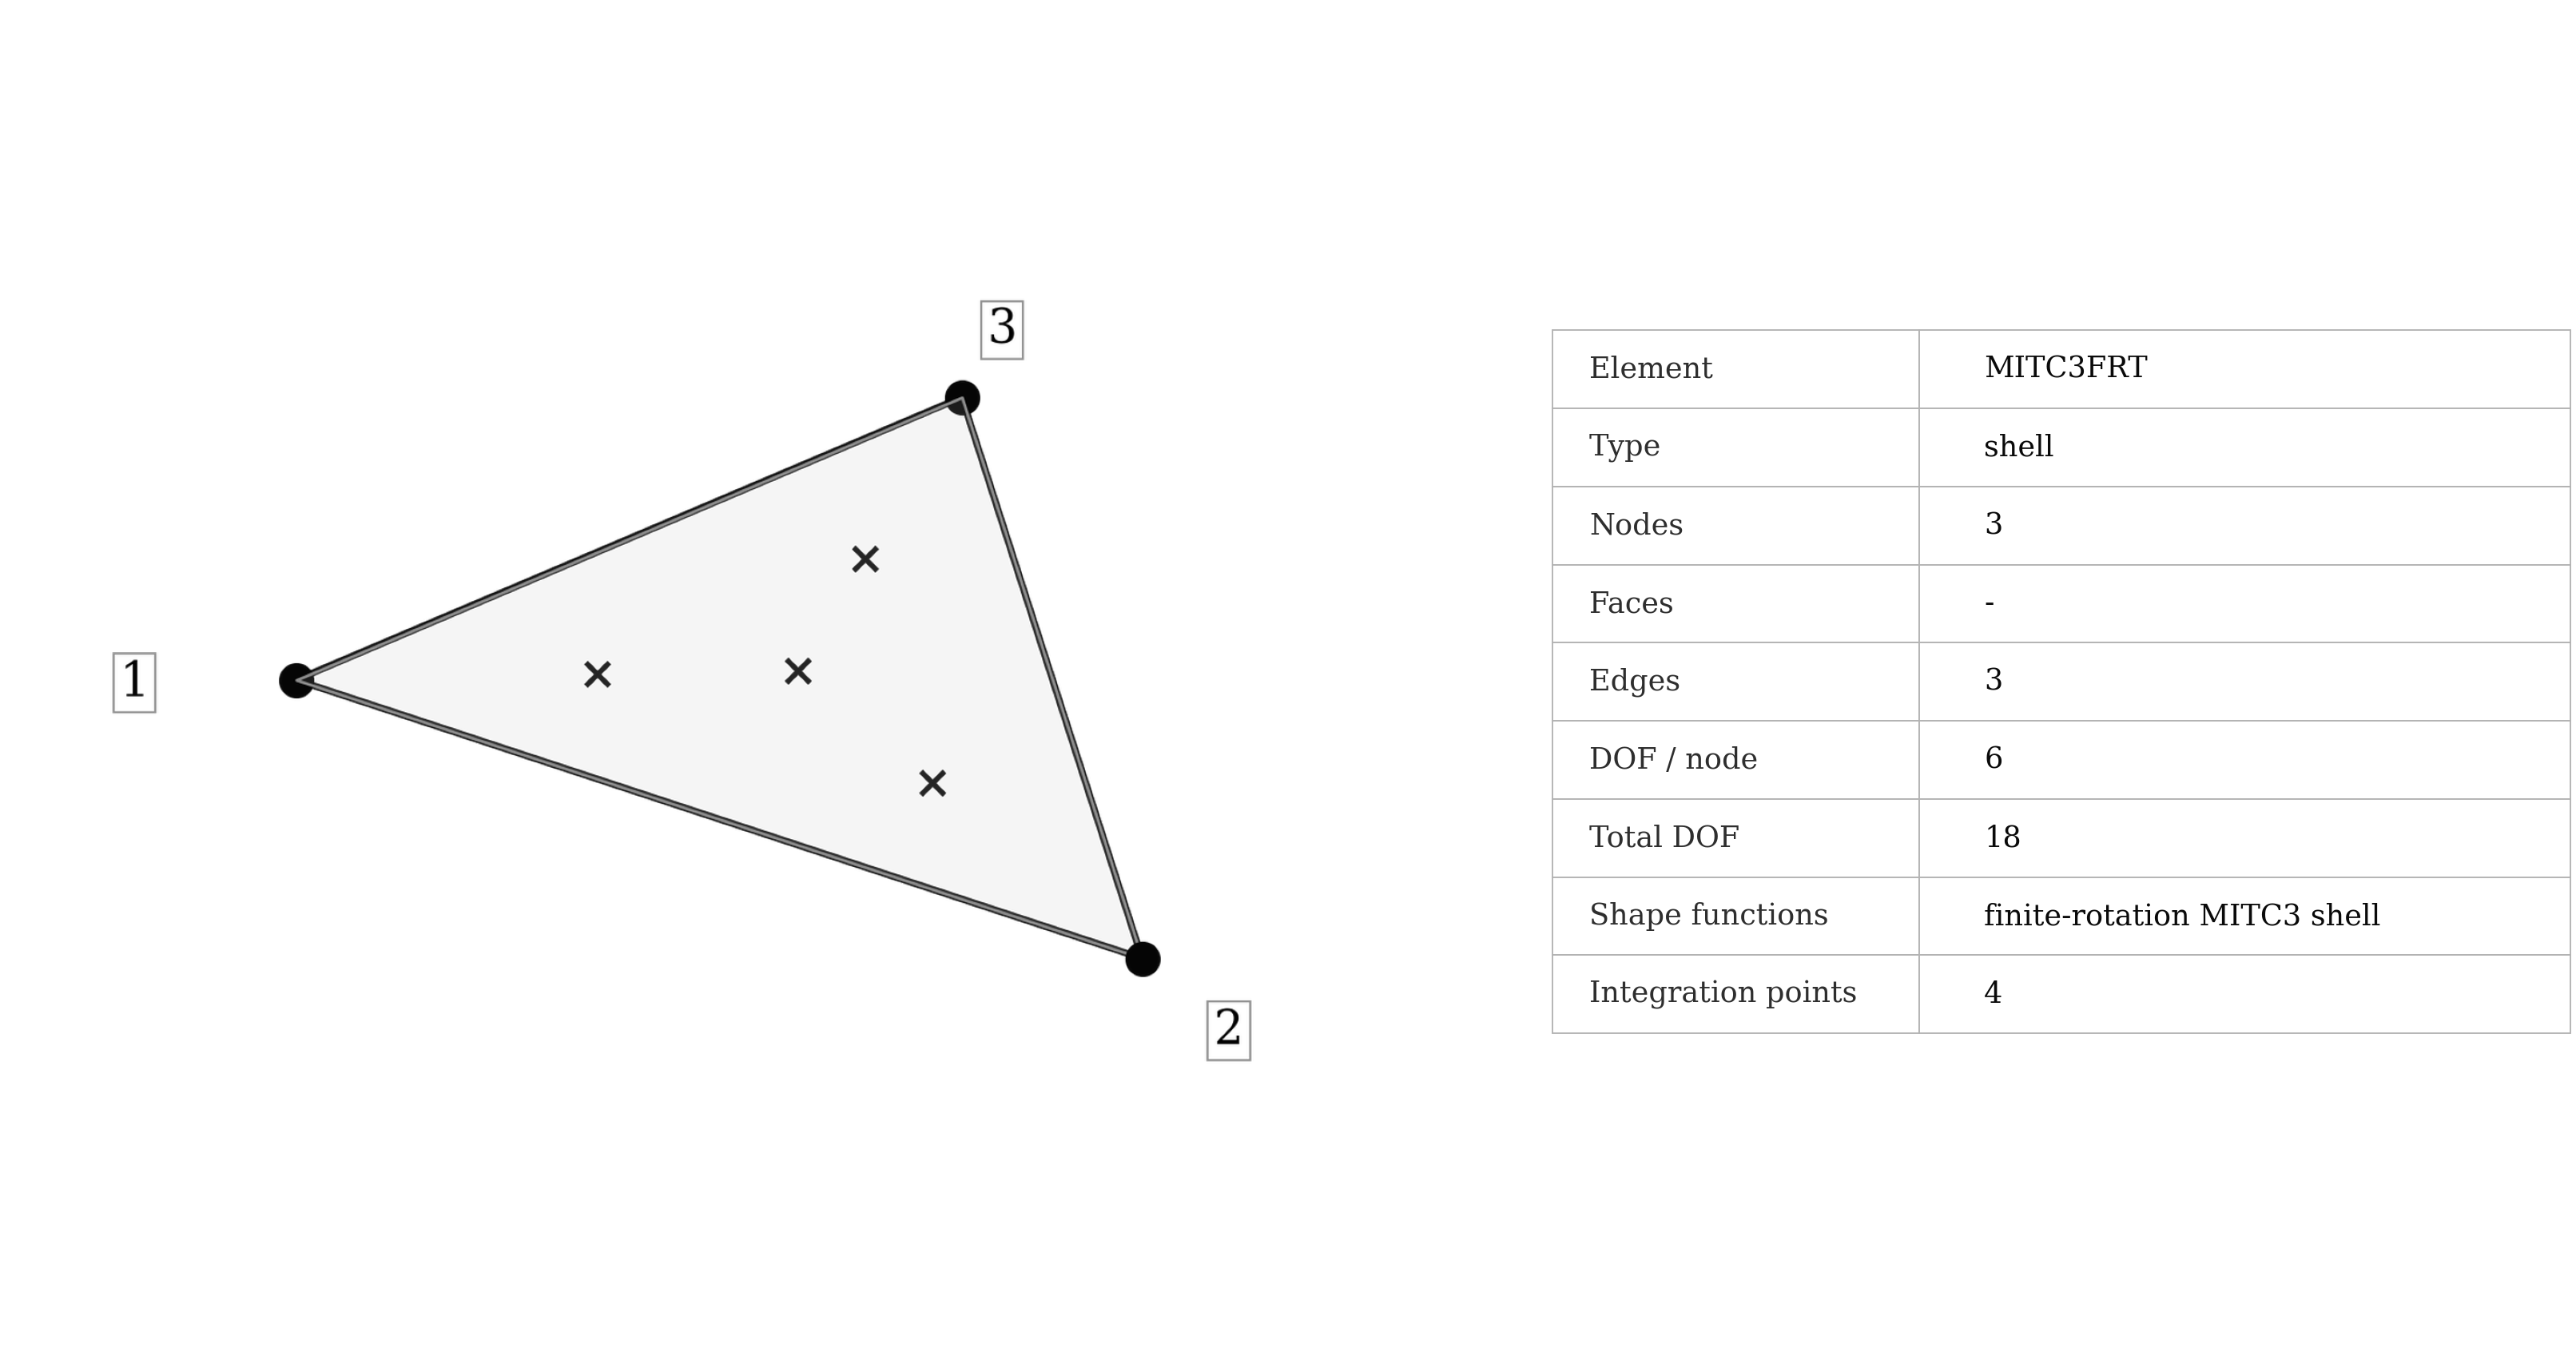
\includegraphics[width=0.76\linewidth]{pages/figures/element_schematics/mitc3frt_schematic.png}
    \caption{\val{MITC3FRT} finite-rotation triangular shell.}
\end{figure}

\begin{syntax}
*ELEMENT, TYPE=MITC3FRT, ELSET=<set>
<id>, <n1>, <n2>, <n3>
\end{syntax}

\val{MITC3FRT} is the current three-node finite-rotation shell formulation. It retains the geometric flexibility of triangular shell meshes while using the FRT shell kinematics intended for geometrically nonlinear analysis.

Use it where triangular topology is unavoidable or convenient: irregular shell boundaries, local mesh transitions, complex curved midsurfaces, and imported surface meshes. As with every three-node shell, convergence in bending-dominated regions generally requires more elements than a high-quality quadrilateral mesh.

For imported Abaqus input, both \val{S3} and \val{S3R} are translated to this formulation. The Abaqus suffix therefore does not select a separate reduced-integration implementation inside FEMaster.

\clearpage
\section{\val{S4}: legacy 4-node quadrilateral shell}

\begin{figure}[H]
    \centering
    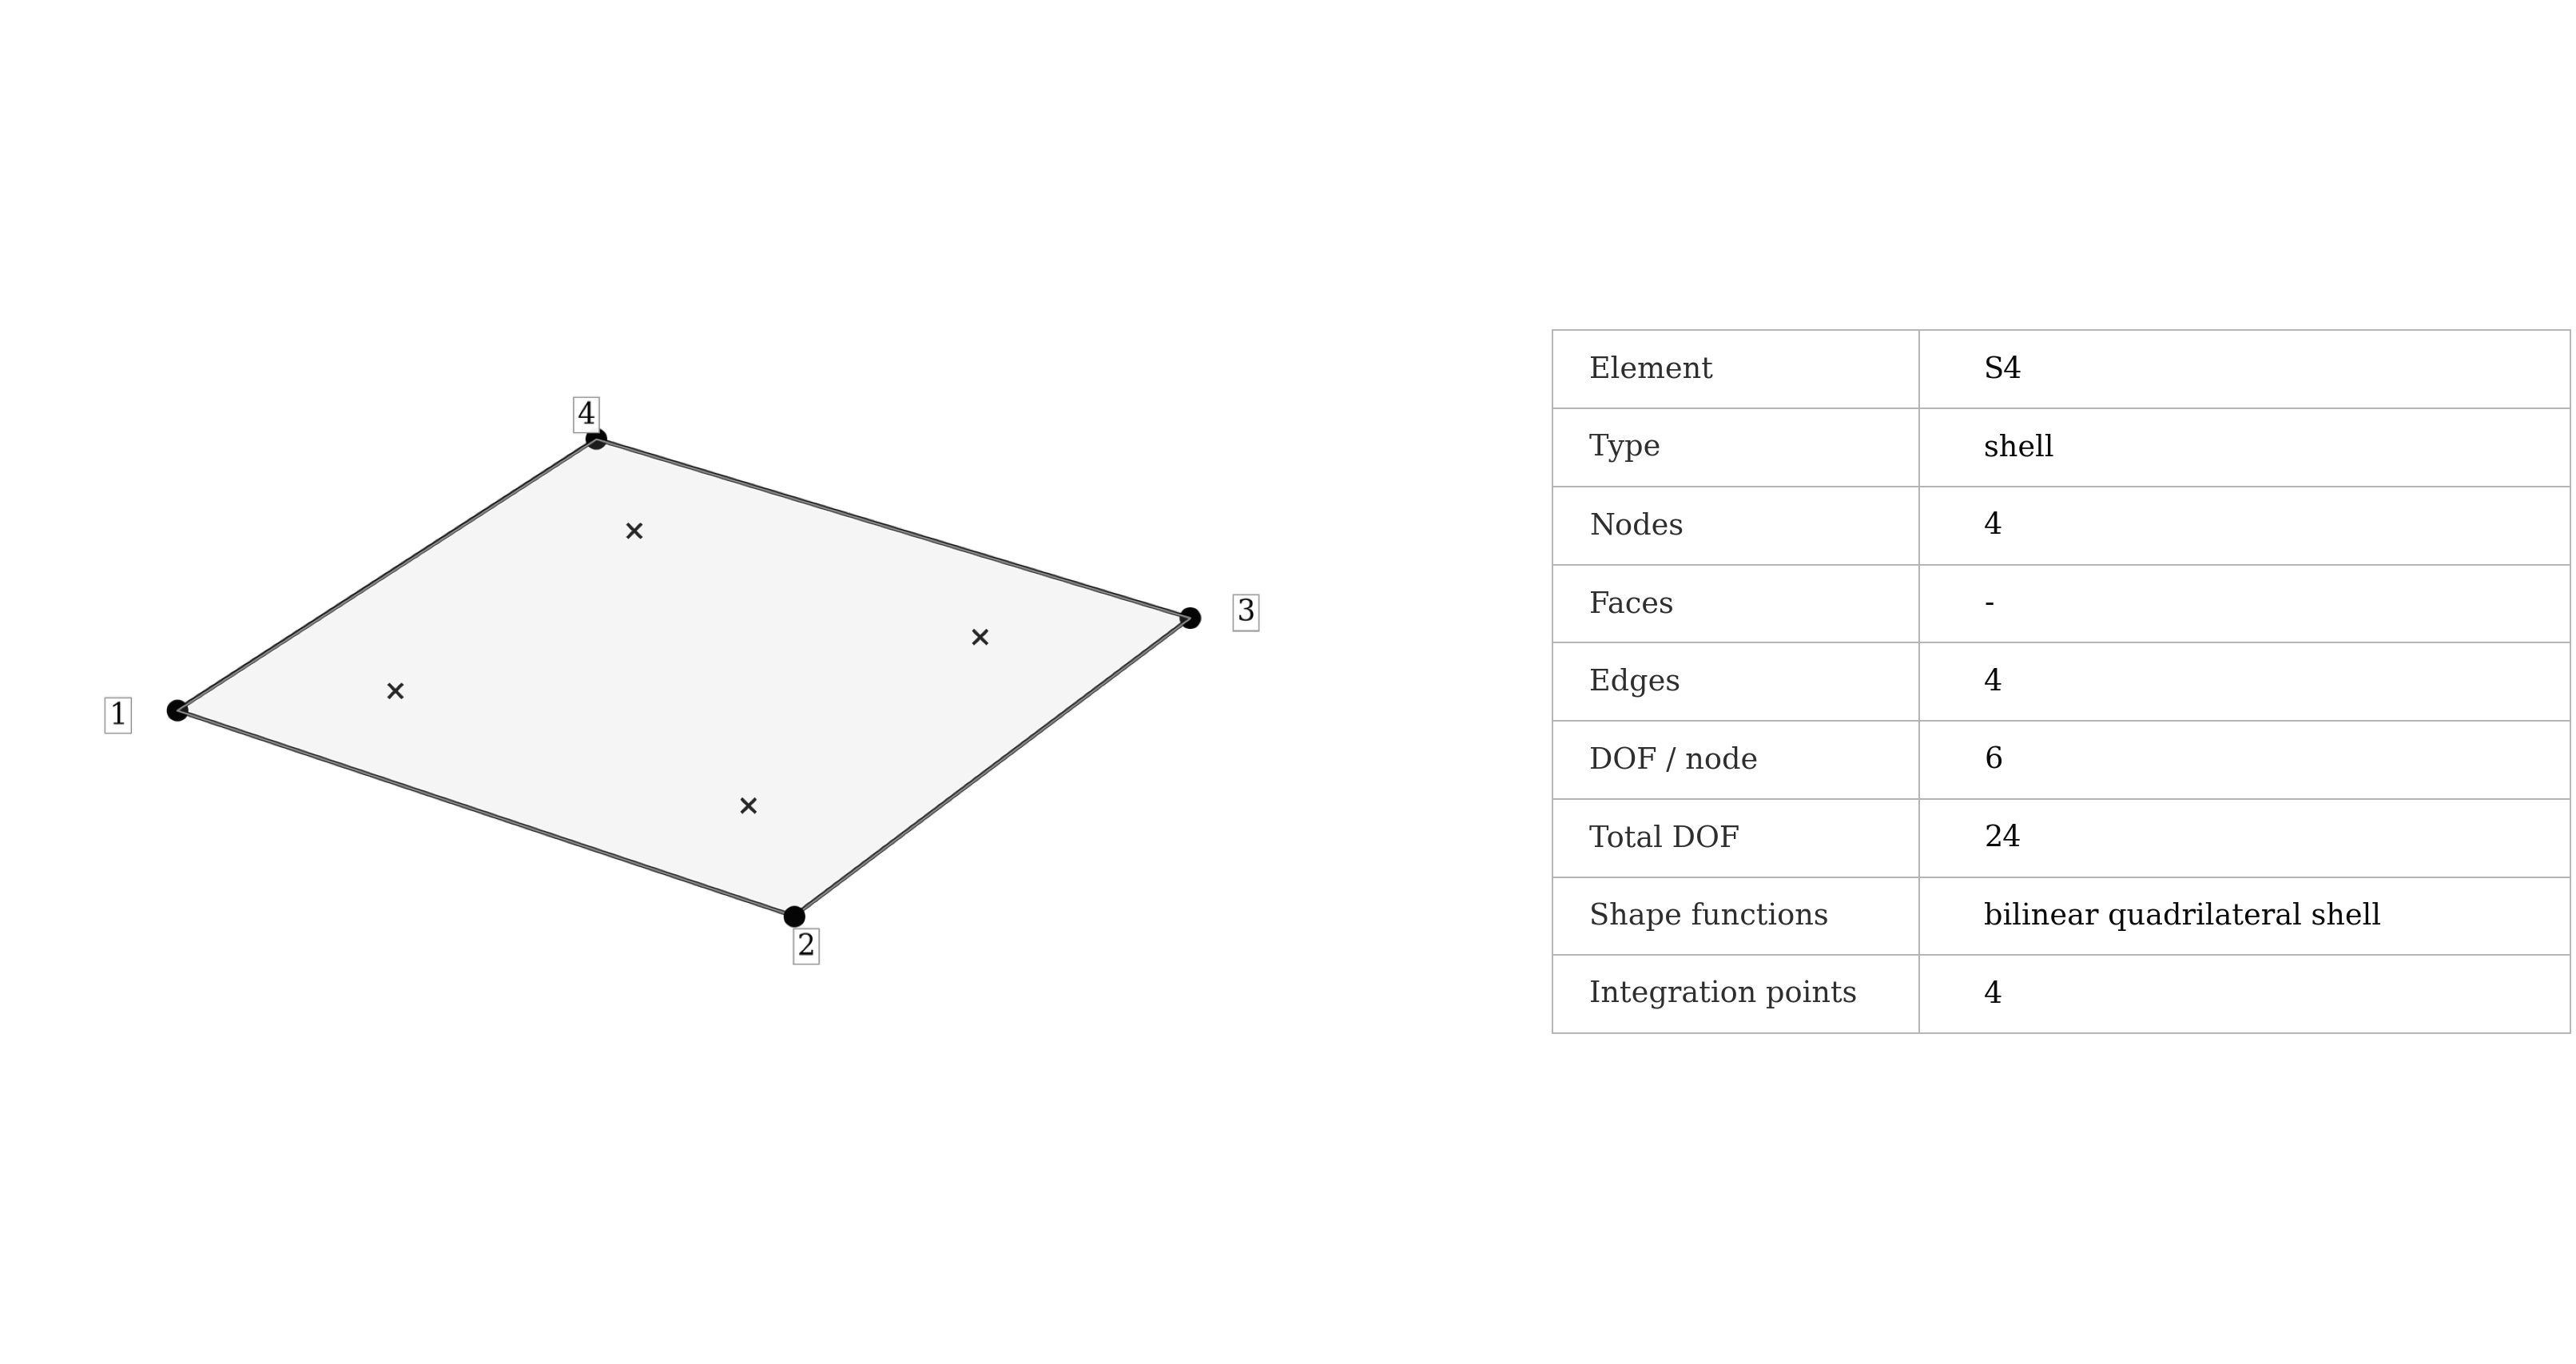
\includegraphics[width=0.78\linewidth]{pages/figures/element_schematics/s4_schematic.png}
    \caption{\val{S4} quadrilateral shell topology.}
\end{figure}

\begin{syntax}
*ELEMENT, TYPE=S4, ELSET=<set>
<id>, <n1>, <n2>, <n3>, <n4>
\end{syntax}

Native \val{S4} is the legacy four-node quadrilateral shell. Quadrilateral topology is attractive for plates, webs, skins, and other surfaces with two natural in-plane directions, but this specific legacy formulation should not be the default for new FEMaster models.

The low-order formulation can suffer severe transverse-shear locking in thin bending-dominated problems. A coarse \val{S4} mesh may therefore appear dramatically too stiff while still satisfying equilibrium. Refining the mesh reduces this problem but is generally less efficient than choosing an appropriate MITC formulation.

Use \val{MITC4FRT} for new four-node shell models. Keep \val{S4} for compatibility, regression comparisons, or controlled studies of the legacy formulation.

\clearpage
\section{\val{MITC4}: legacy 4-node shell with tied shear interpolation}

\begin{figure}[H]
    \centering
    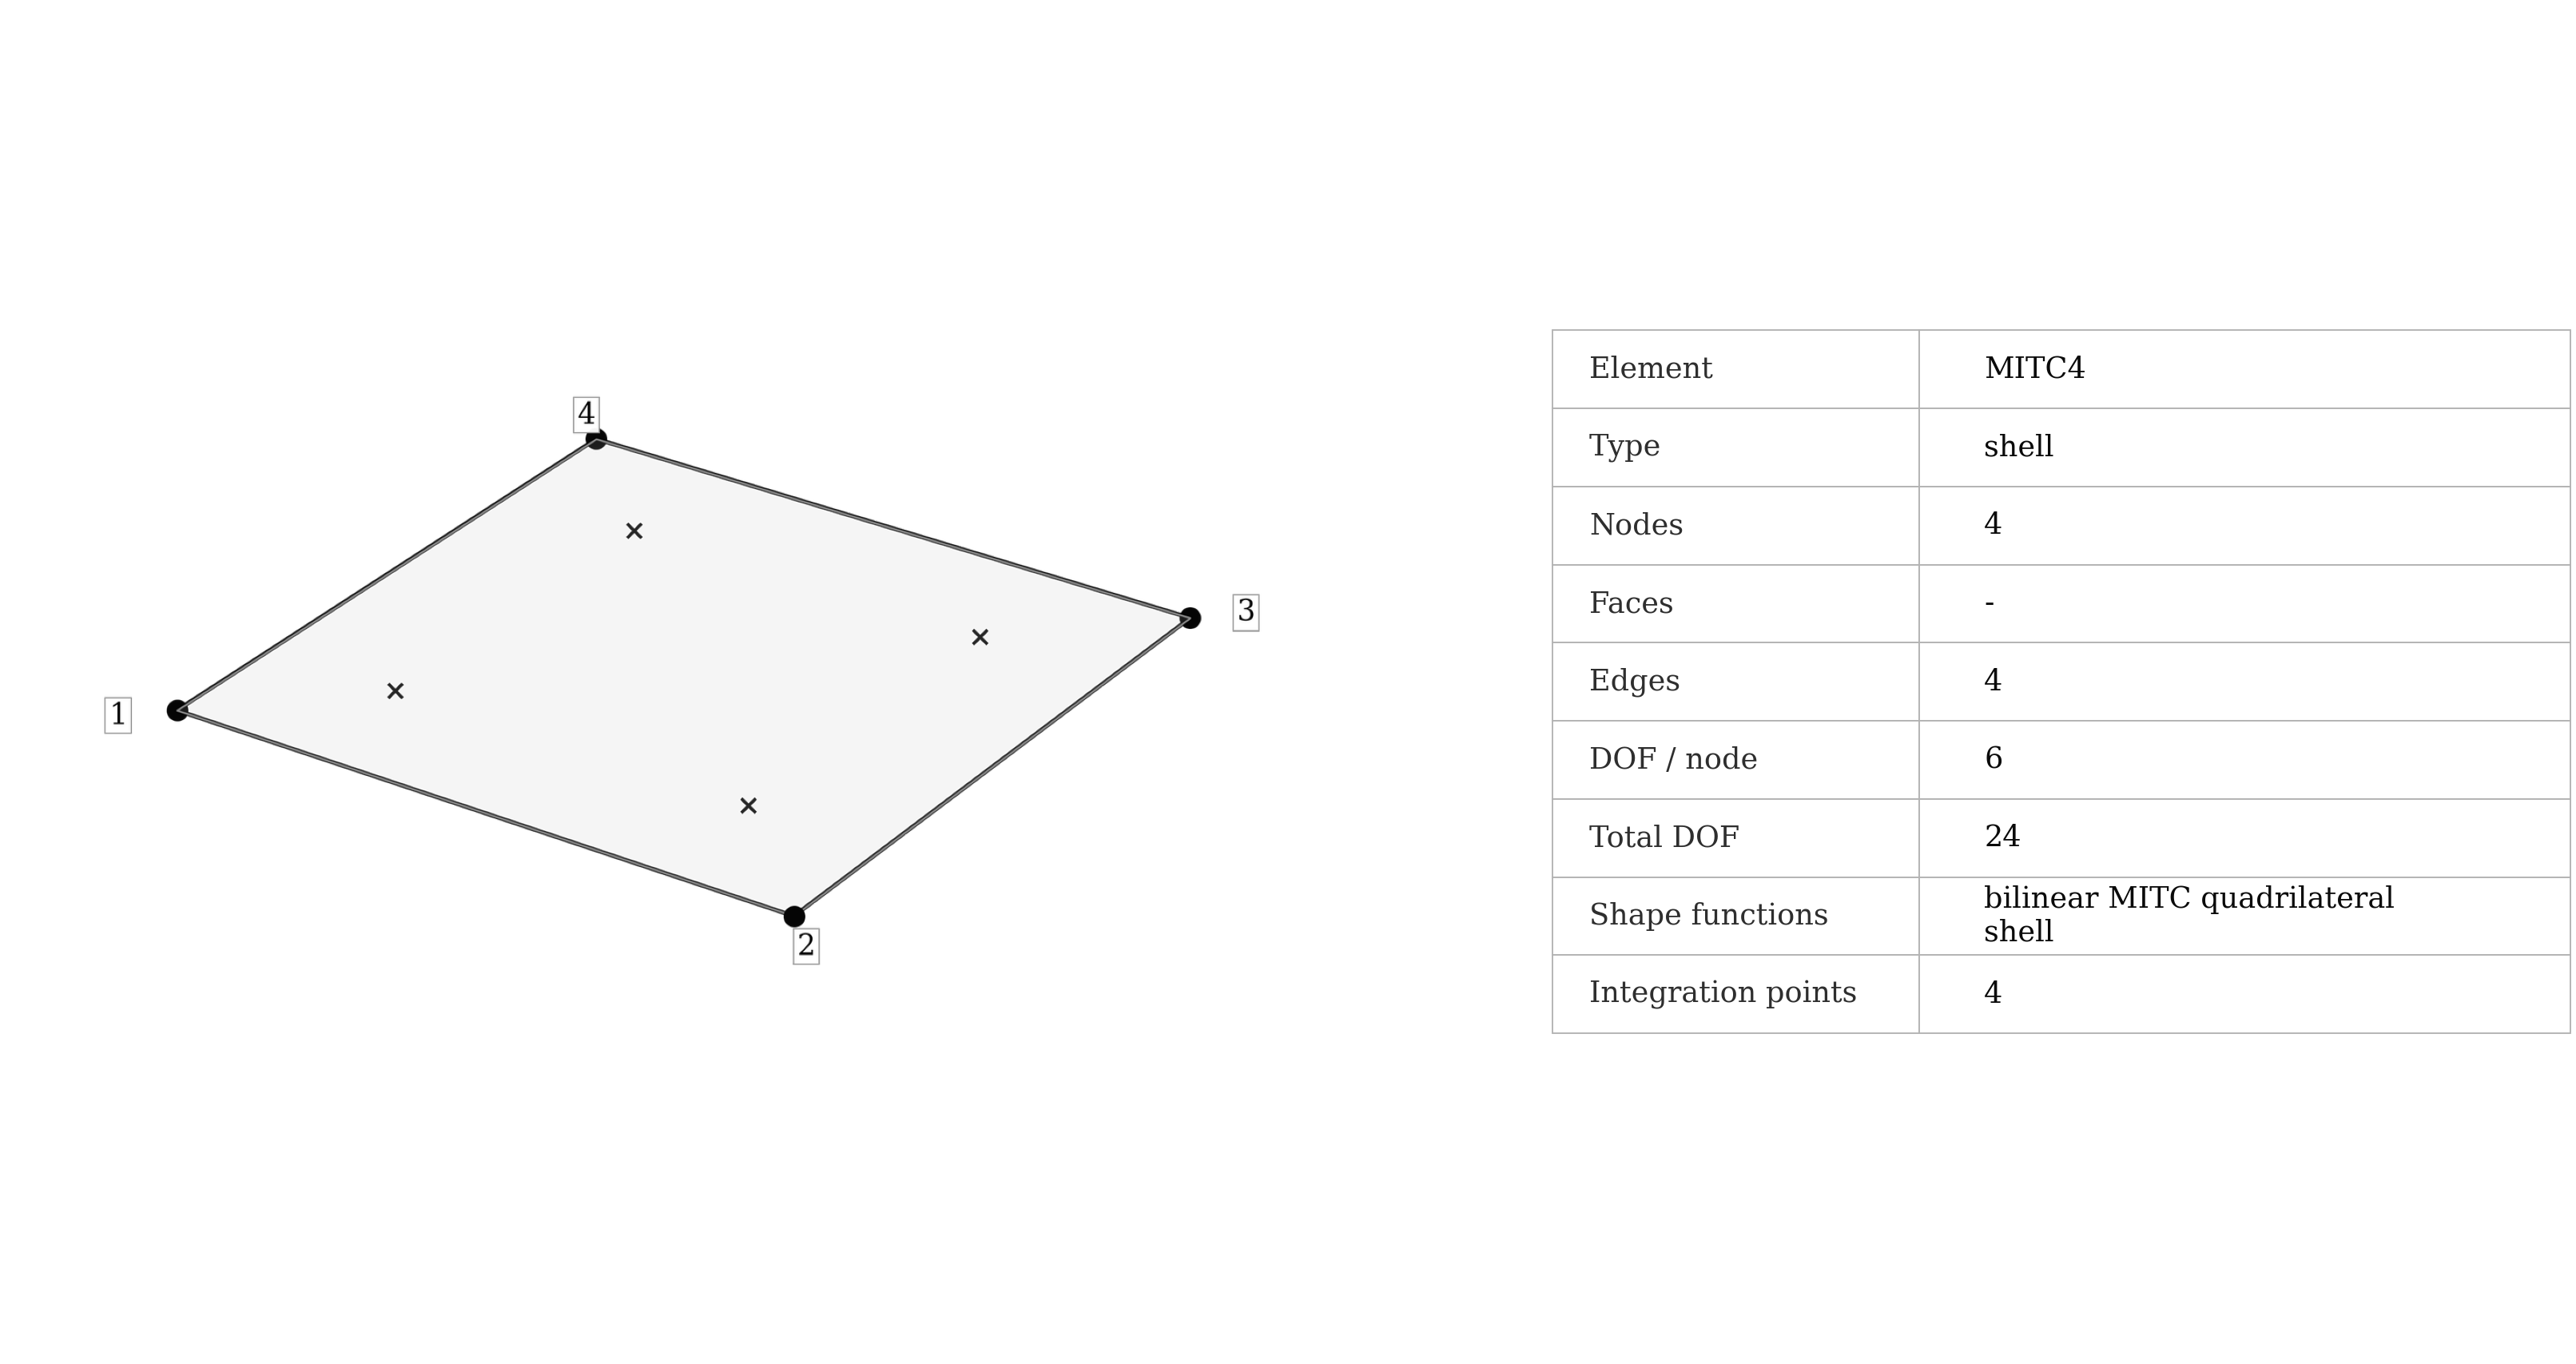
\includegraphics[width=0.78\linewidth]{pages/figures/element_schematics/mitc4_schematic.png}
    \caption{\val{MITC4} shell with MITC transverse-shear interpolation.}
\end{figure}

\begin{syntax}
*ELEMENT, TYPE=MITC4, ELSET=<set>
<id>, <n1>, <n2>, <n3>, <n4>
\end{syntax}

\val{MITC4} uses the same four-node topology as \val{S4} but replaces the direct low-order transverse-shear interpolation with MITC-style tied shear interpolation. The purpose is to suppress the artificial shear constraint responsible for locking in thin bending problems.

This element historically provided much better thin-shell bending behaviour than \val{S4} on coarse meshes. It remains useful for regression and linear-formulation comparison, but new models should normally use \val{MITC4FRT}, which combines the corresponding low-order MITC idea with the current finite-rotation shell formulation.

MITC interpolation does not make a quadrilateral insensitive to mesh quality. Excessive warping, skew, poor aspect ratio, and inconsistent normals can still degrade both stiffness and stress recovery.

\clearpage
\section{\val{MITC4FRT}: finite-rotation 4-node MITC shell}

\begin{figure}[H]
    \centering
    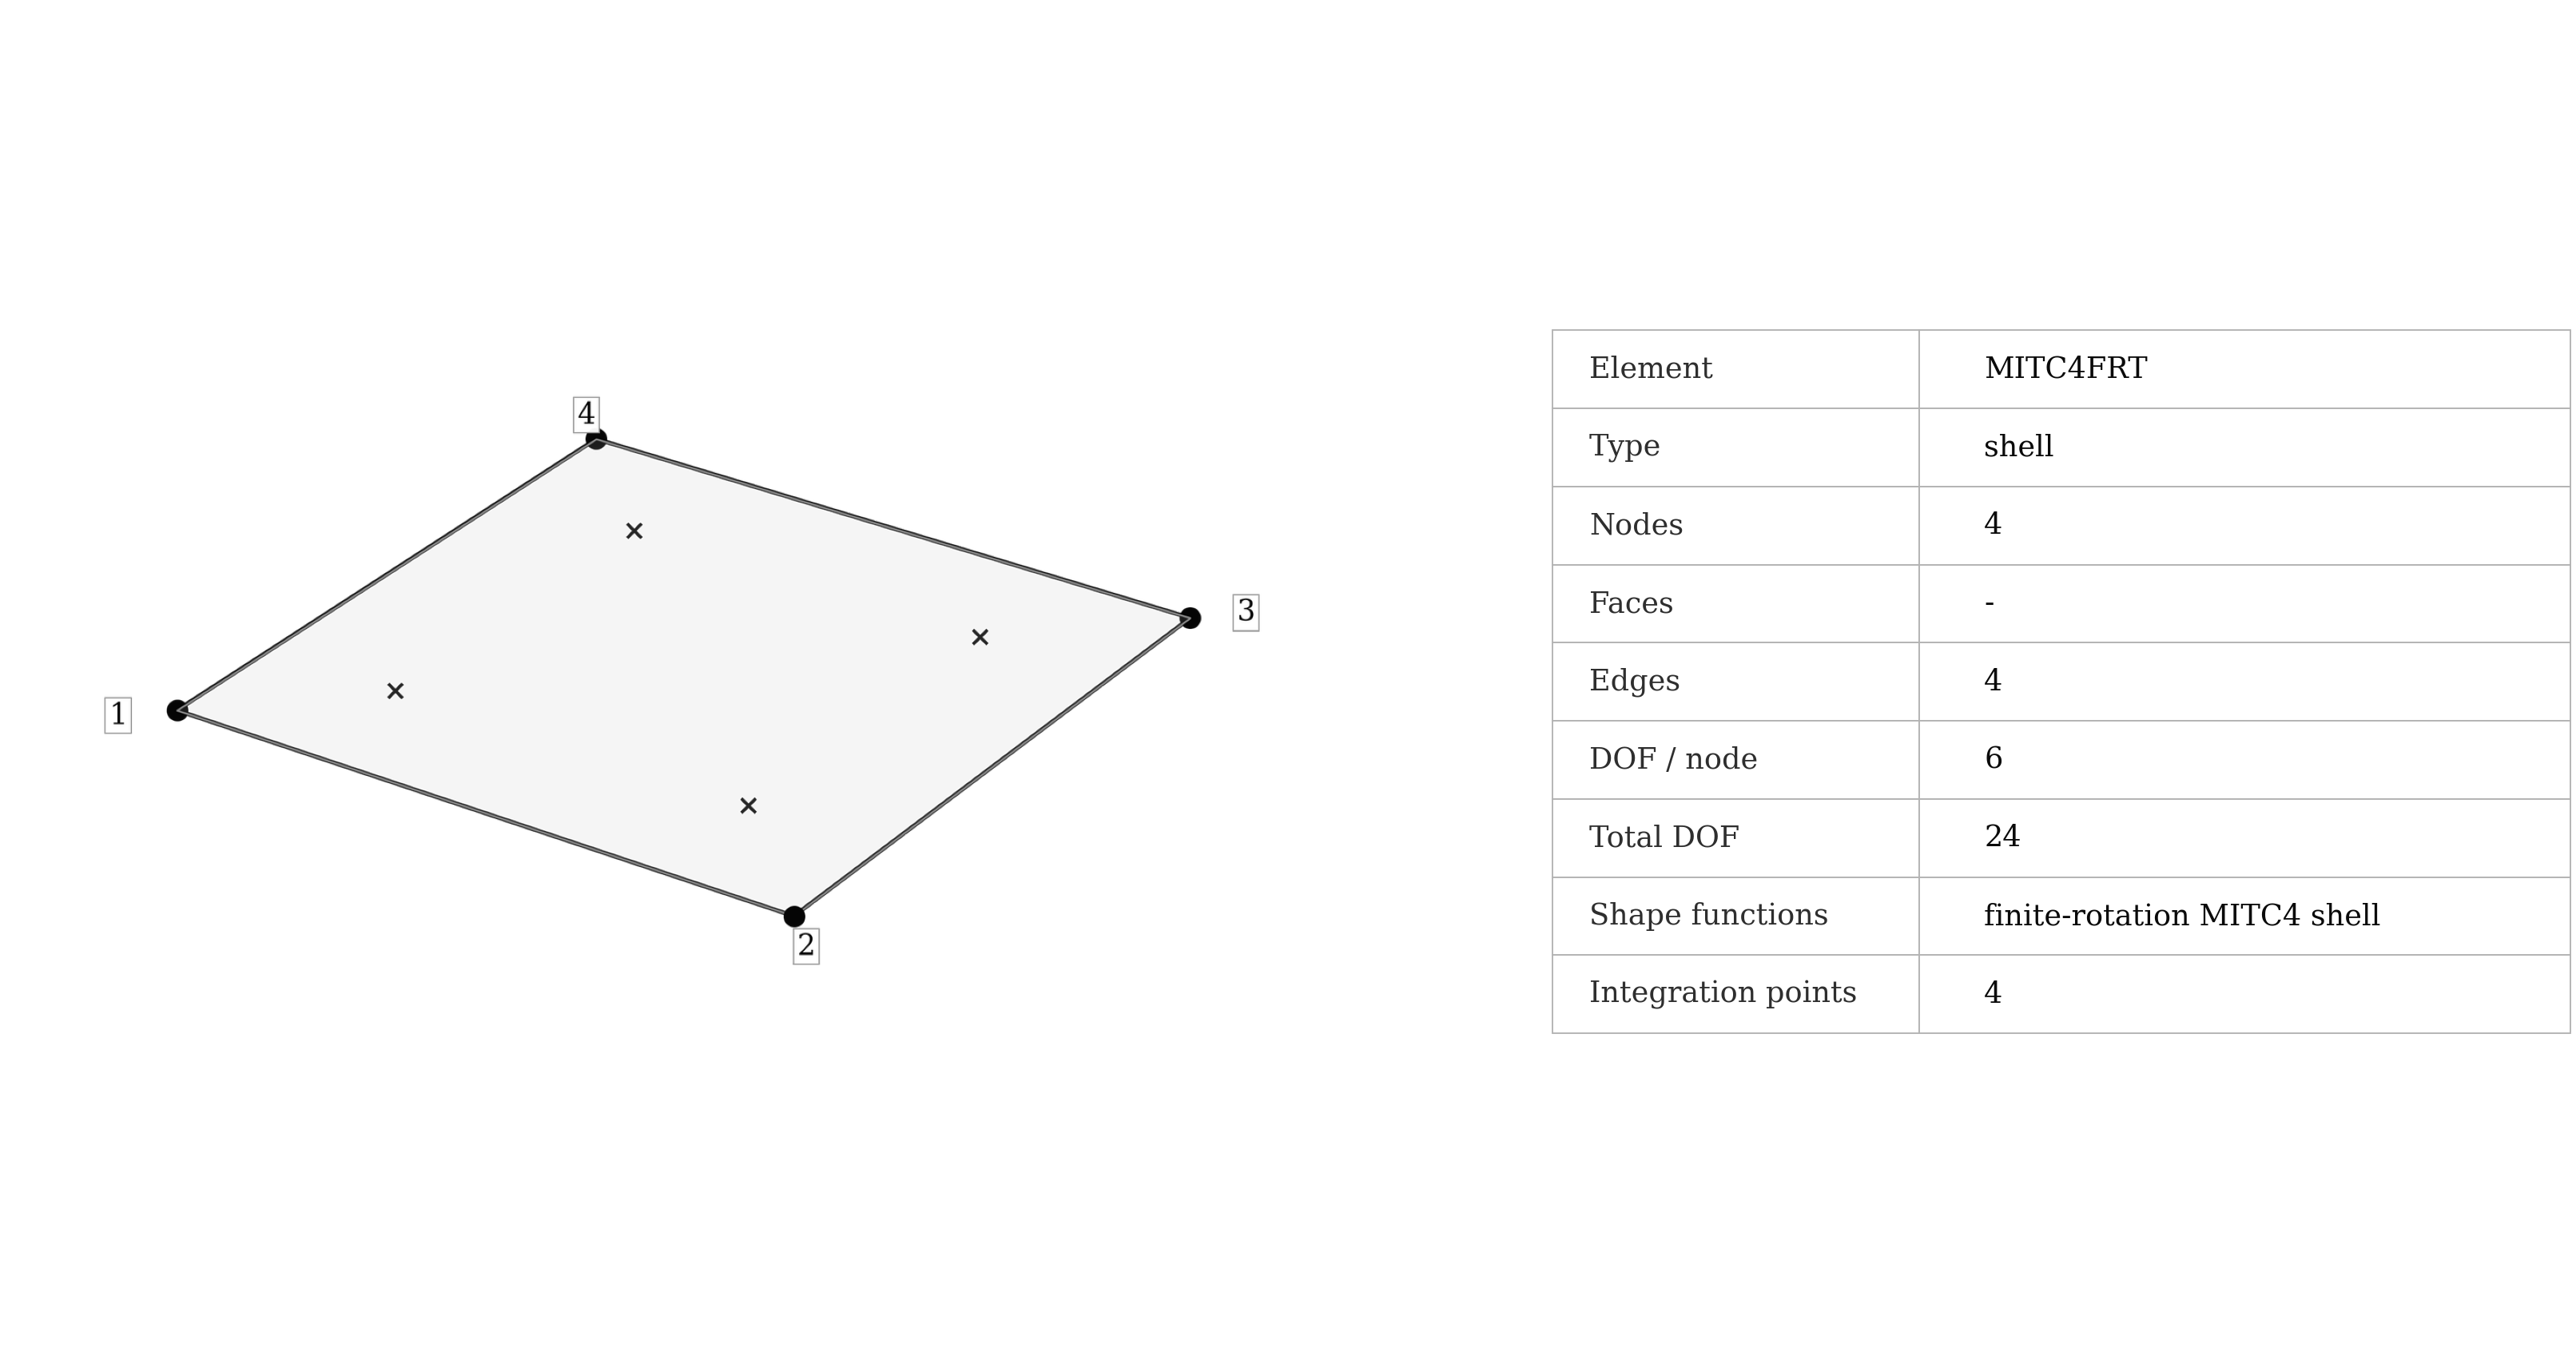
\includegraphics[width=0.78\linewidth]{pages/figures/element_schematics/mitc4frt_schematic.png}
    \caption{\val{MITC4FRT} finite-rotation quadrilateral shell.}
\end{figure}

\begin{syntax}
*ELEMENT, TYPE=MITC4FRT, ELSET=<set>
<id>, <n1>, <n2>, <n3>, <n4>
\end{syntax}

\val{MITC4FRT} is the recommended low-order quadrilateral shell for current FEMaster models. It uses finite-rotation shell kinematics and MITC transverse-shear interpolation, making it suitable for thin-shell bending as well as geometrically nonlinear deformation where rotations become large.

The four-node topology keeps mesh generation and element cost modest. It is a good default for panels, webs, skins, shells of moderate curvature, and large shell assemblies when a structured or mostly quadrilateral midsurface mesh is available.

Tied shear interpolation addresses shear locking but does not eliminate geometric discretization error. Curved surfaces still require sufficient mesh density, strongly warped quadrilaterals should be avoided, and nonlinear load paths should be checked using deformed shapes, reaction balance, and convergence under refinement.

The supported Abaqus labels \val{S4} and \val{S4R} are both translated to \val{MITC4FRT}.

\clearpage
\section{\val{S6}: legacy 6-node triangular shell}

\begin{figure}[H]
    \centering
    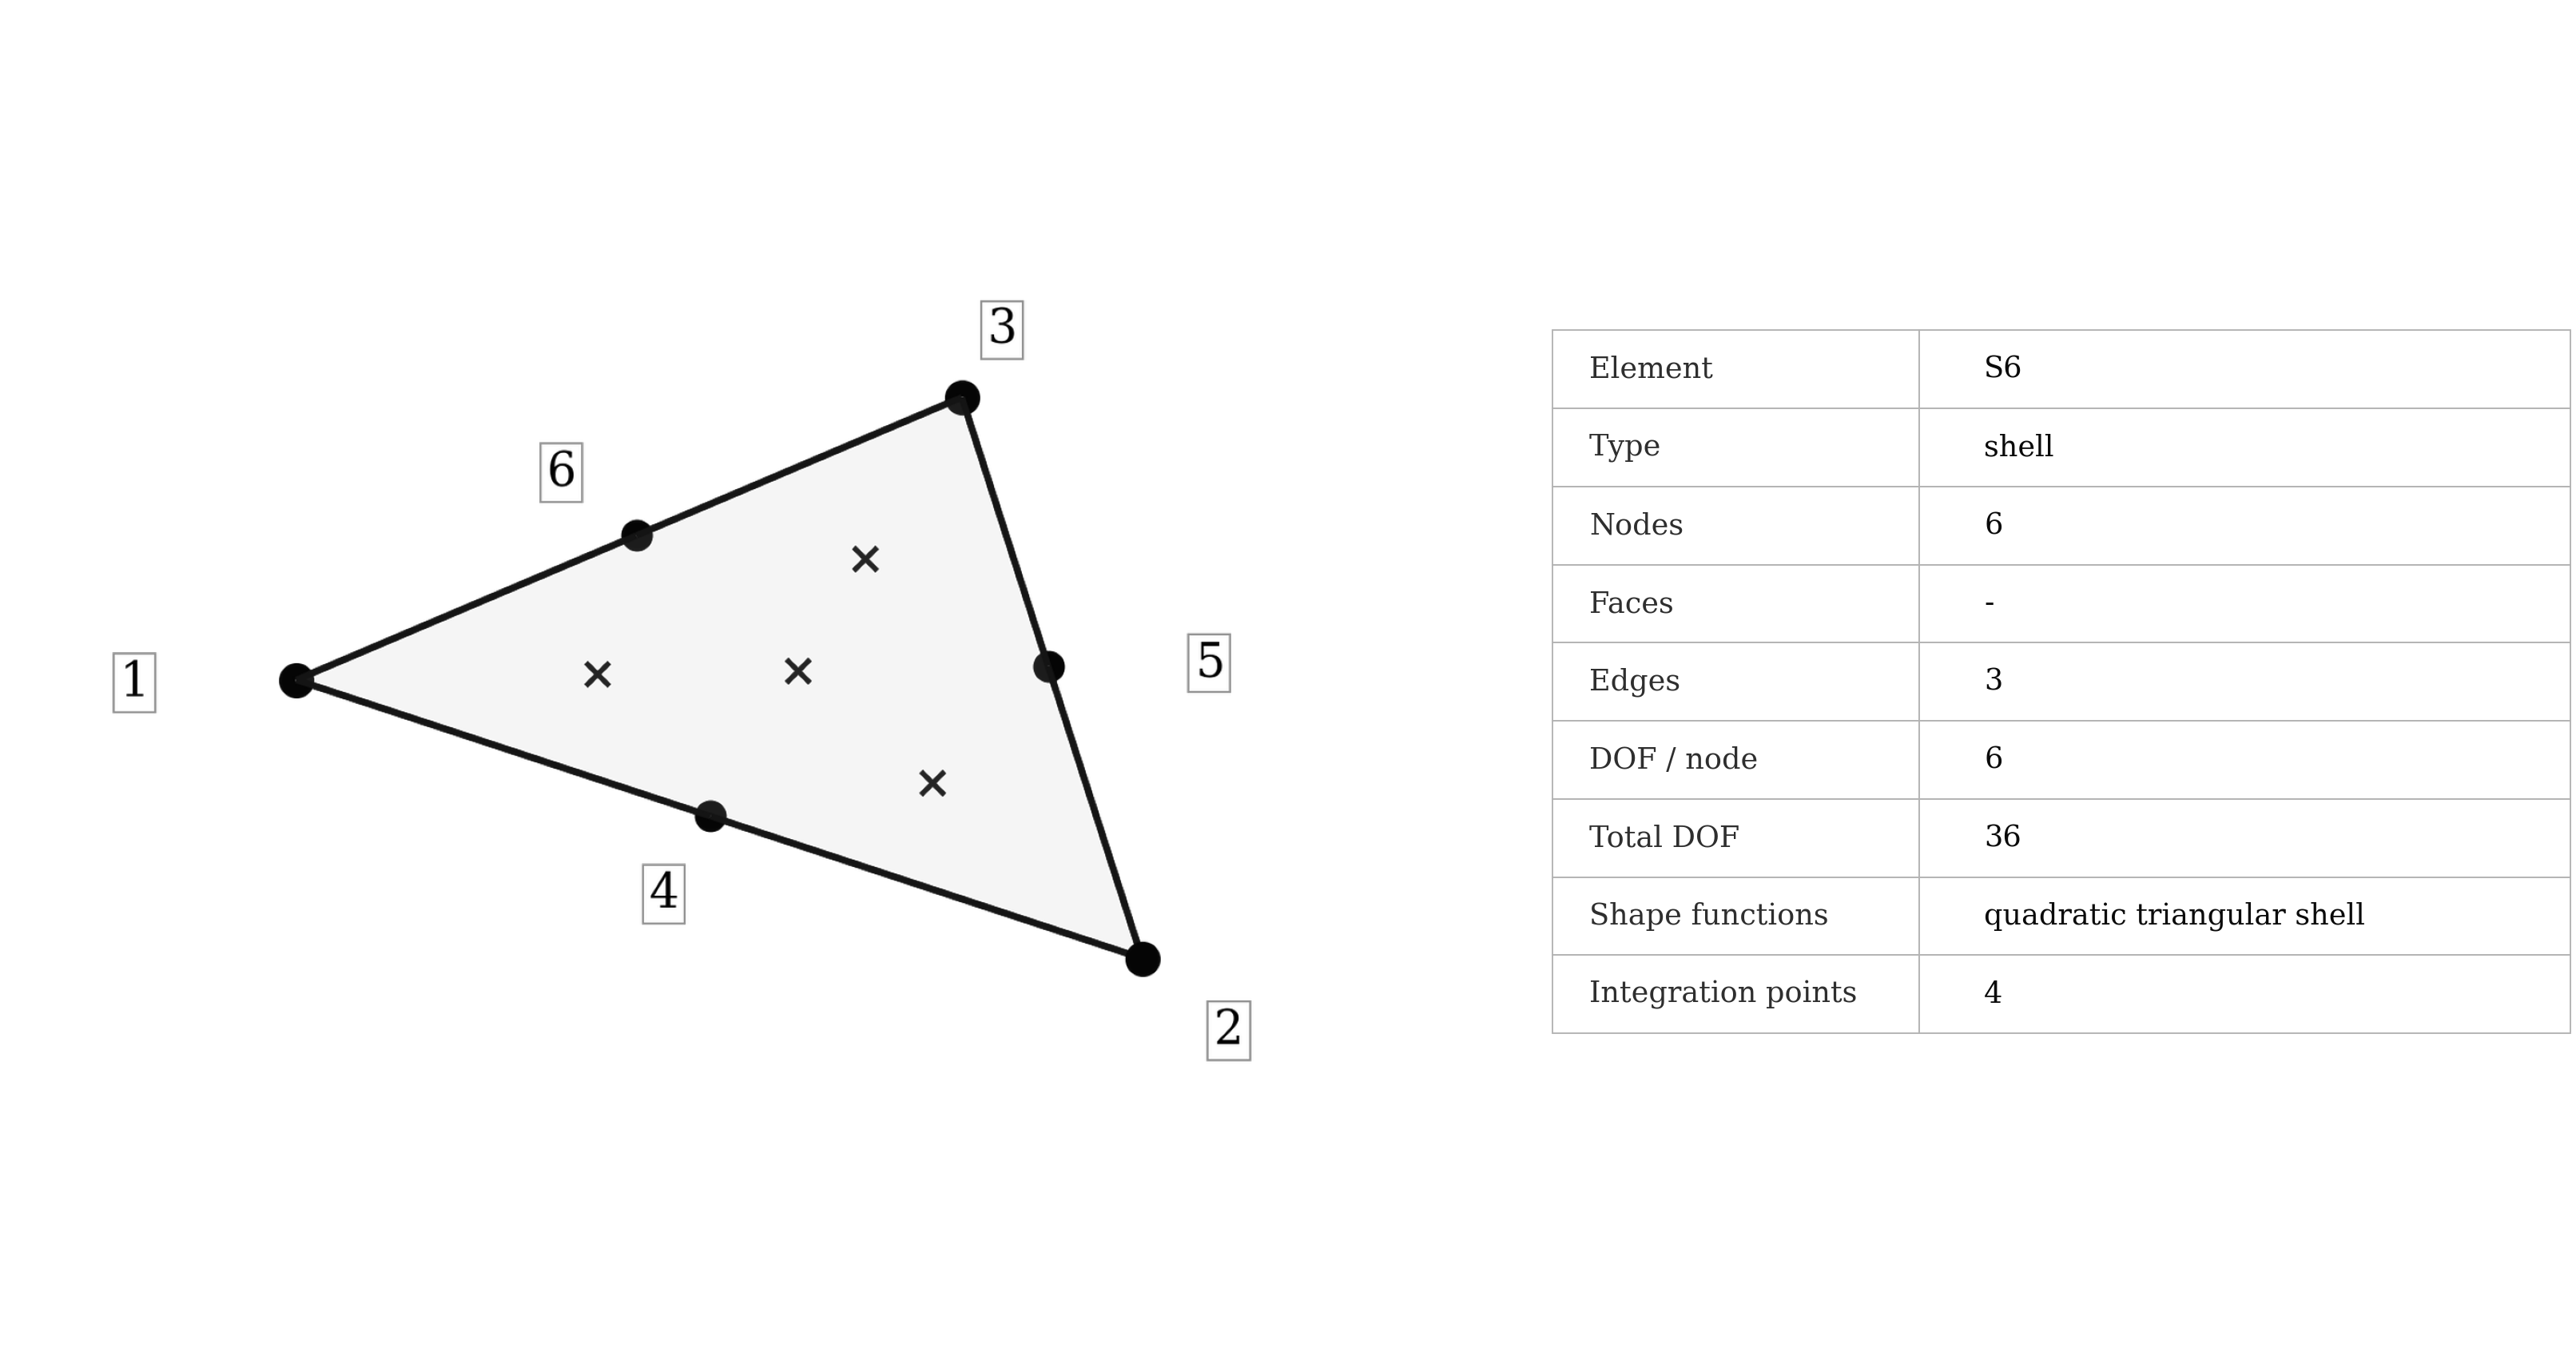
\includegraphics[width=0.78\linewidth]{pages/figures/element_schematics/s6_schematic.png}
    \caption{\val{S6} quadratic triangular shell.}
\end{figure}

\begin{syntax}
*ELEMENT, TYPE=S6, ELSET=<set>
<id>, <n1>, <n2>, <n3>, <n4>, <n5>, <n6>
\end{syntax}

Native \val{S6} is the legacy six-node quadratic triangular shell. The midside nodes improve geometric representation and allow a smoother in-plane and bending interpolation than \val{S3}. It is useful in older curved triangular shell meshes and for comparisons with the corresponding FRT formulation.

For new analyses, use \val{MITC6FRT}. The higher-order triangle can represent curved boundaries effectively, but the location of midside nodes and the quality of the parent triangle remain important. Badly curved or highly skewed elements can create poor mappings despite the higher interpolation order.

\clearpage
\section{\val{MITC6FRT}: finite-rotation 6-node shell}

\begin{figure}[H]
    \centering
    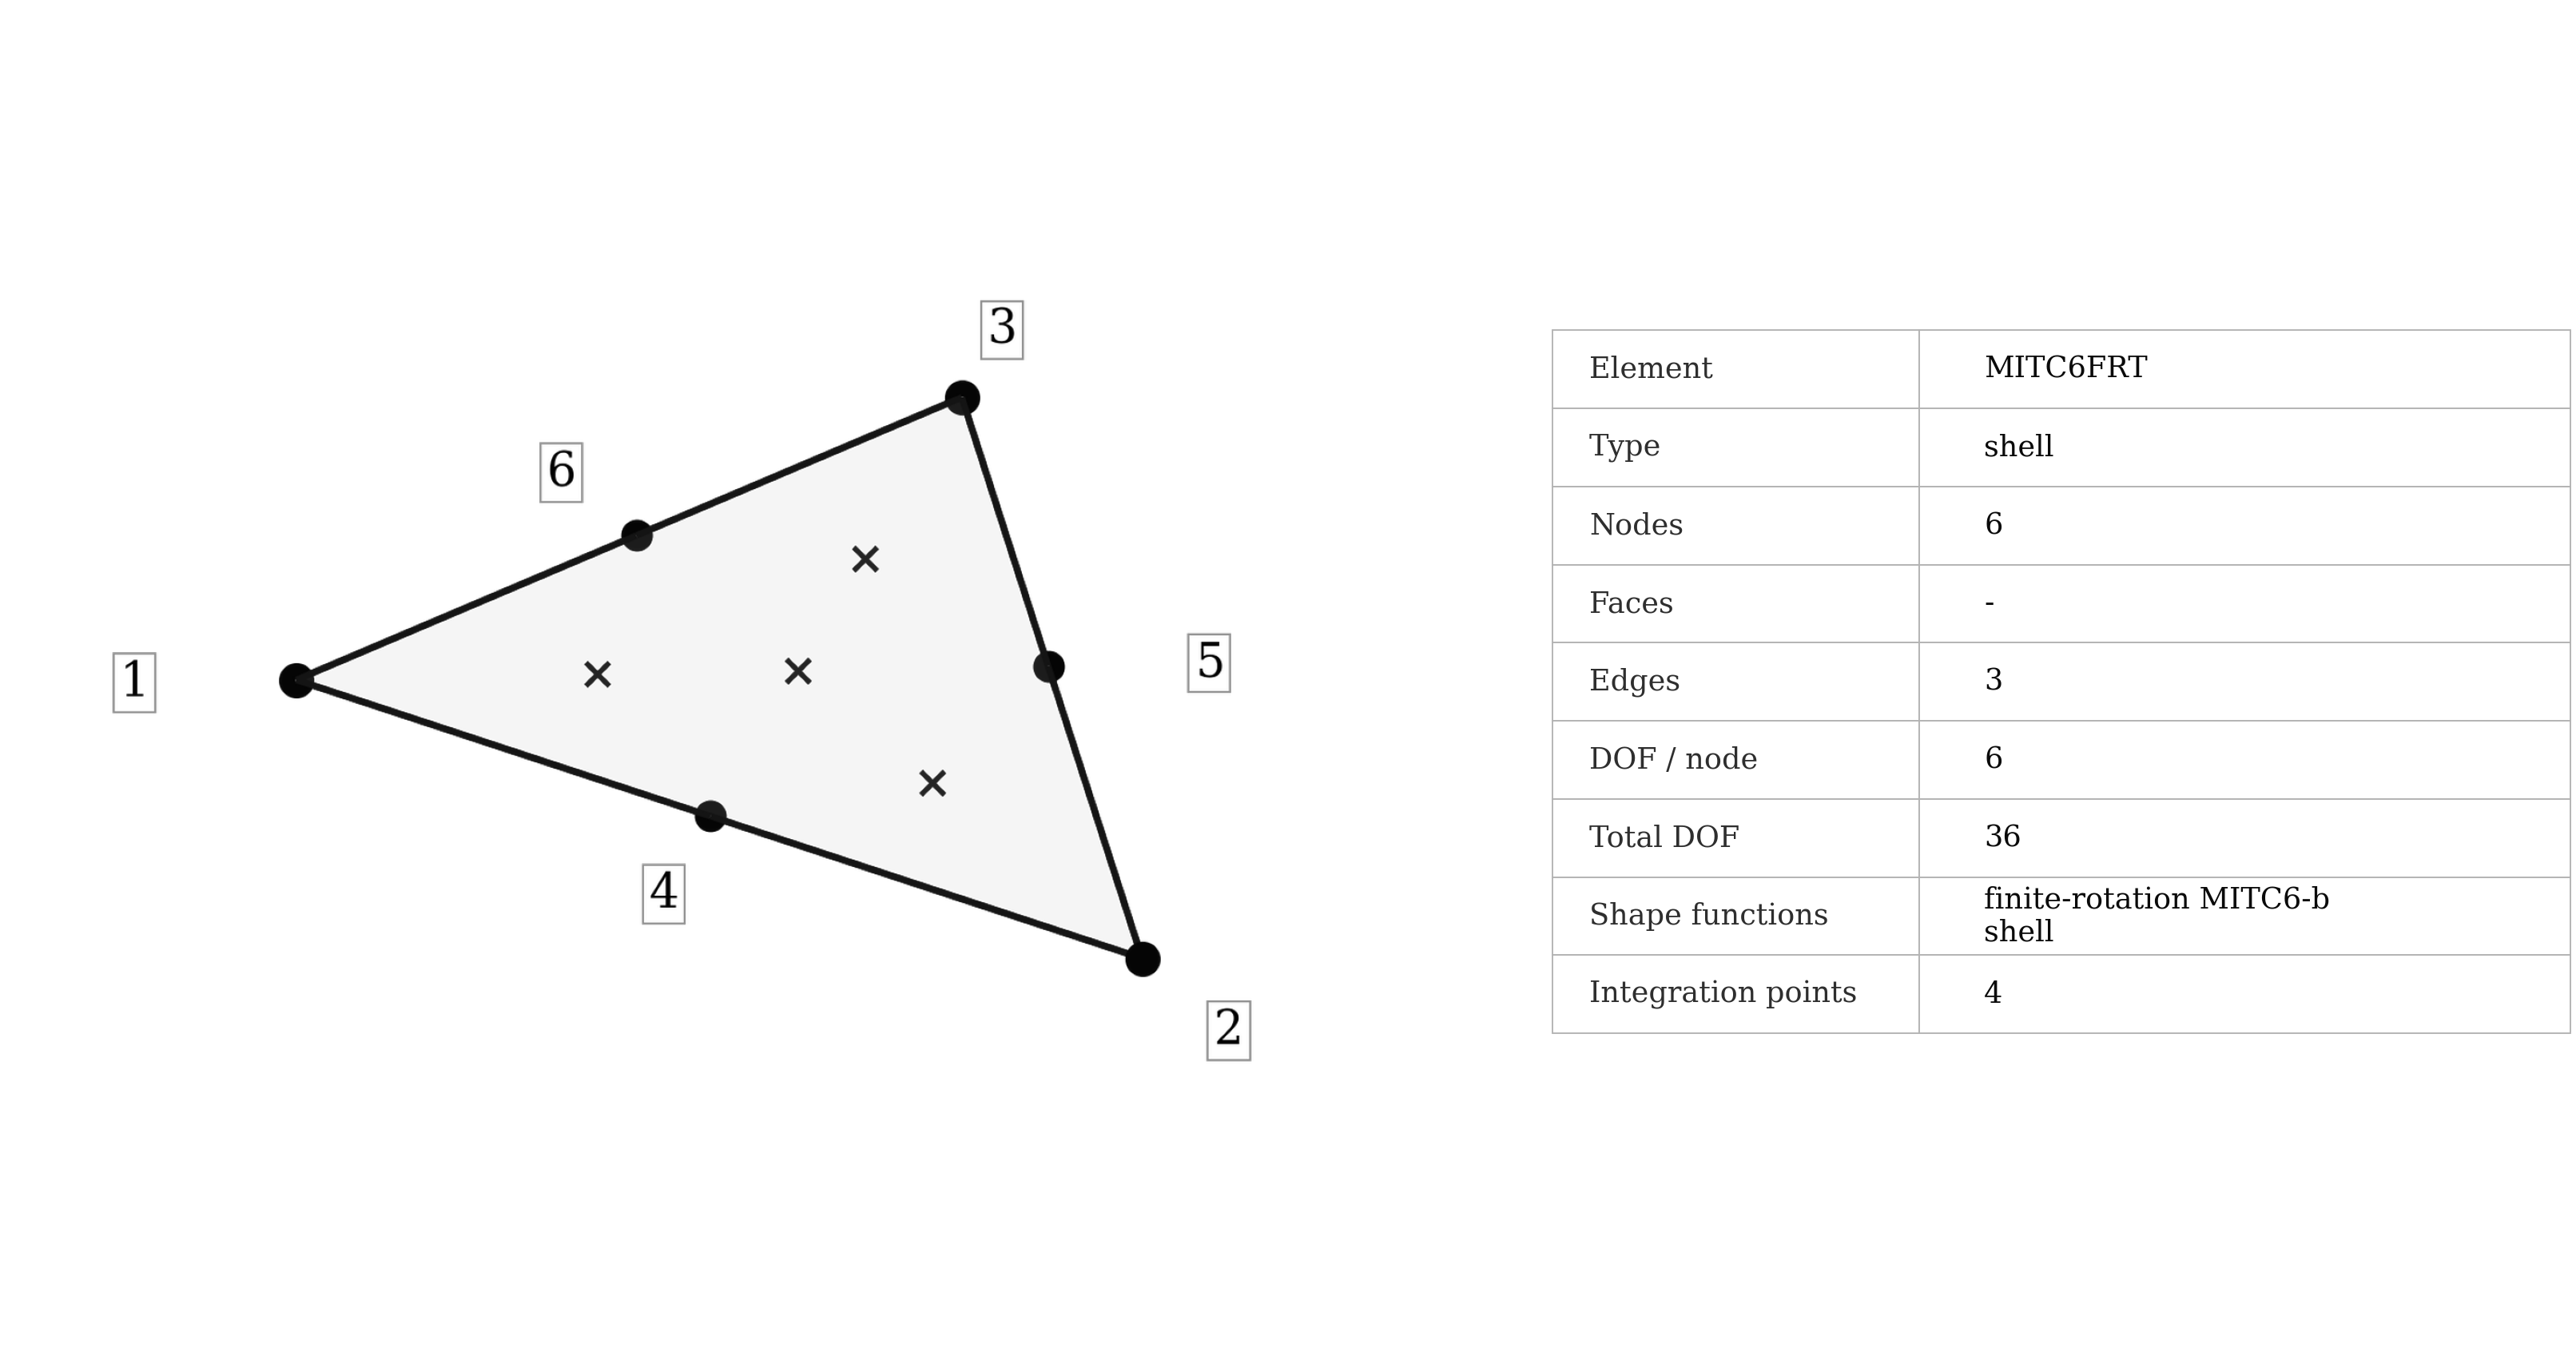
\includegraphics[width=0.78\linewidth]{pages/figures/element_schematics/mitc6frt_schematic.png}
    \caption{\val{MITC6FRT} finite-rotation six-node triangular shell.}
\end{figure}

\begin{syntax}
*ELEMENT, TYPE=MITC6FRT, ELSET=<set>
<id>, <n1>, <n2>, <n3>, <n4>, <n5>, <n6>
\end{syntax}

\val{MITC6FRT} is the current six-node triangular finite-rotation shell. It combines quadratic triangular geometry with the FRT shell formulation and is the preferred triangular choice when a higher-order midsurface description is desired.

The element is well suited to curved shell regions where triangular topology is convenient but a low-order three-node mesh would require excessive refinement. Midside nodes allow curved edges and smoother deformation fields, provided they are positioned consistently with the intended geometry.

Both Abaqus \val{S6} and \val{S6R} are translated to this formulation by the current reader.

\clearpage
\section{\val{S8}: legacy 8-node quadrilateral shell}

\begin{figure}[H]
    \centering
    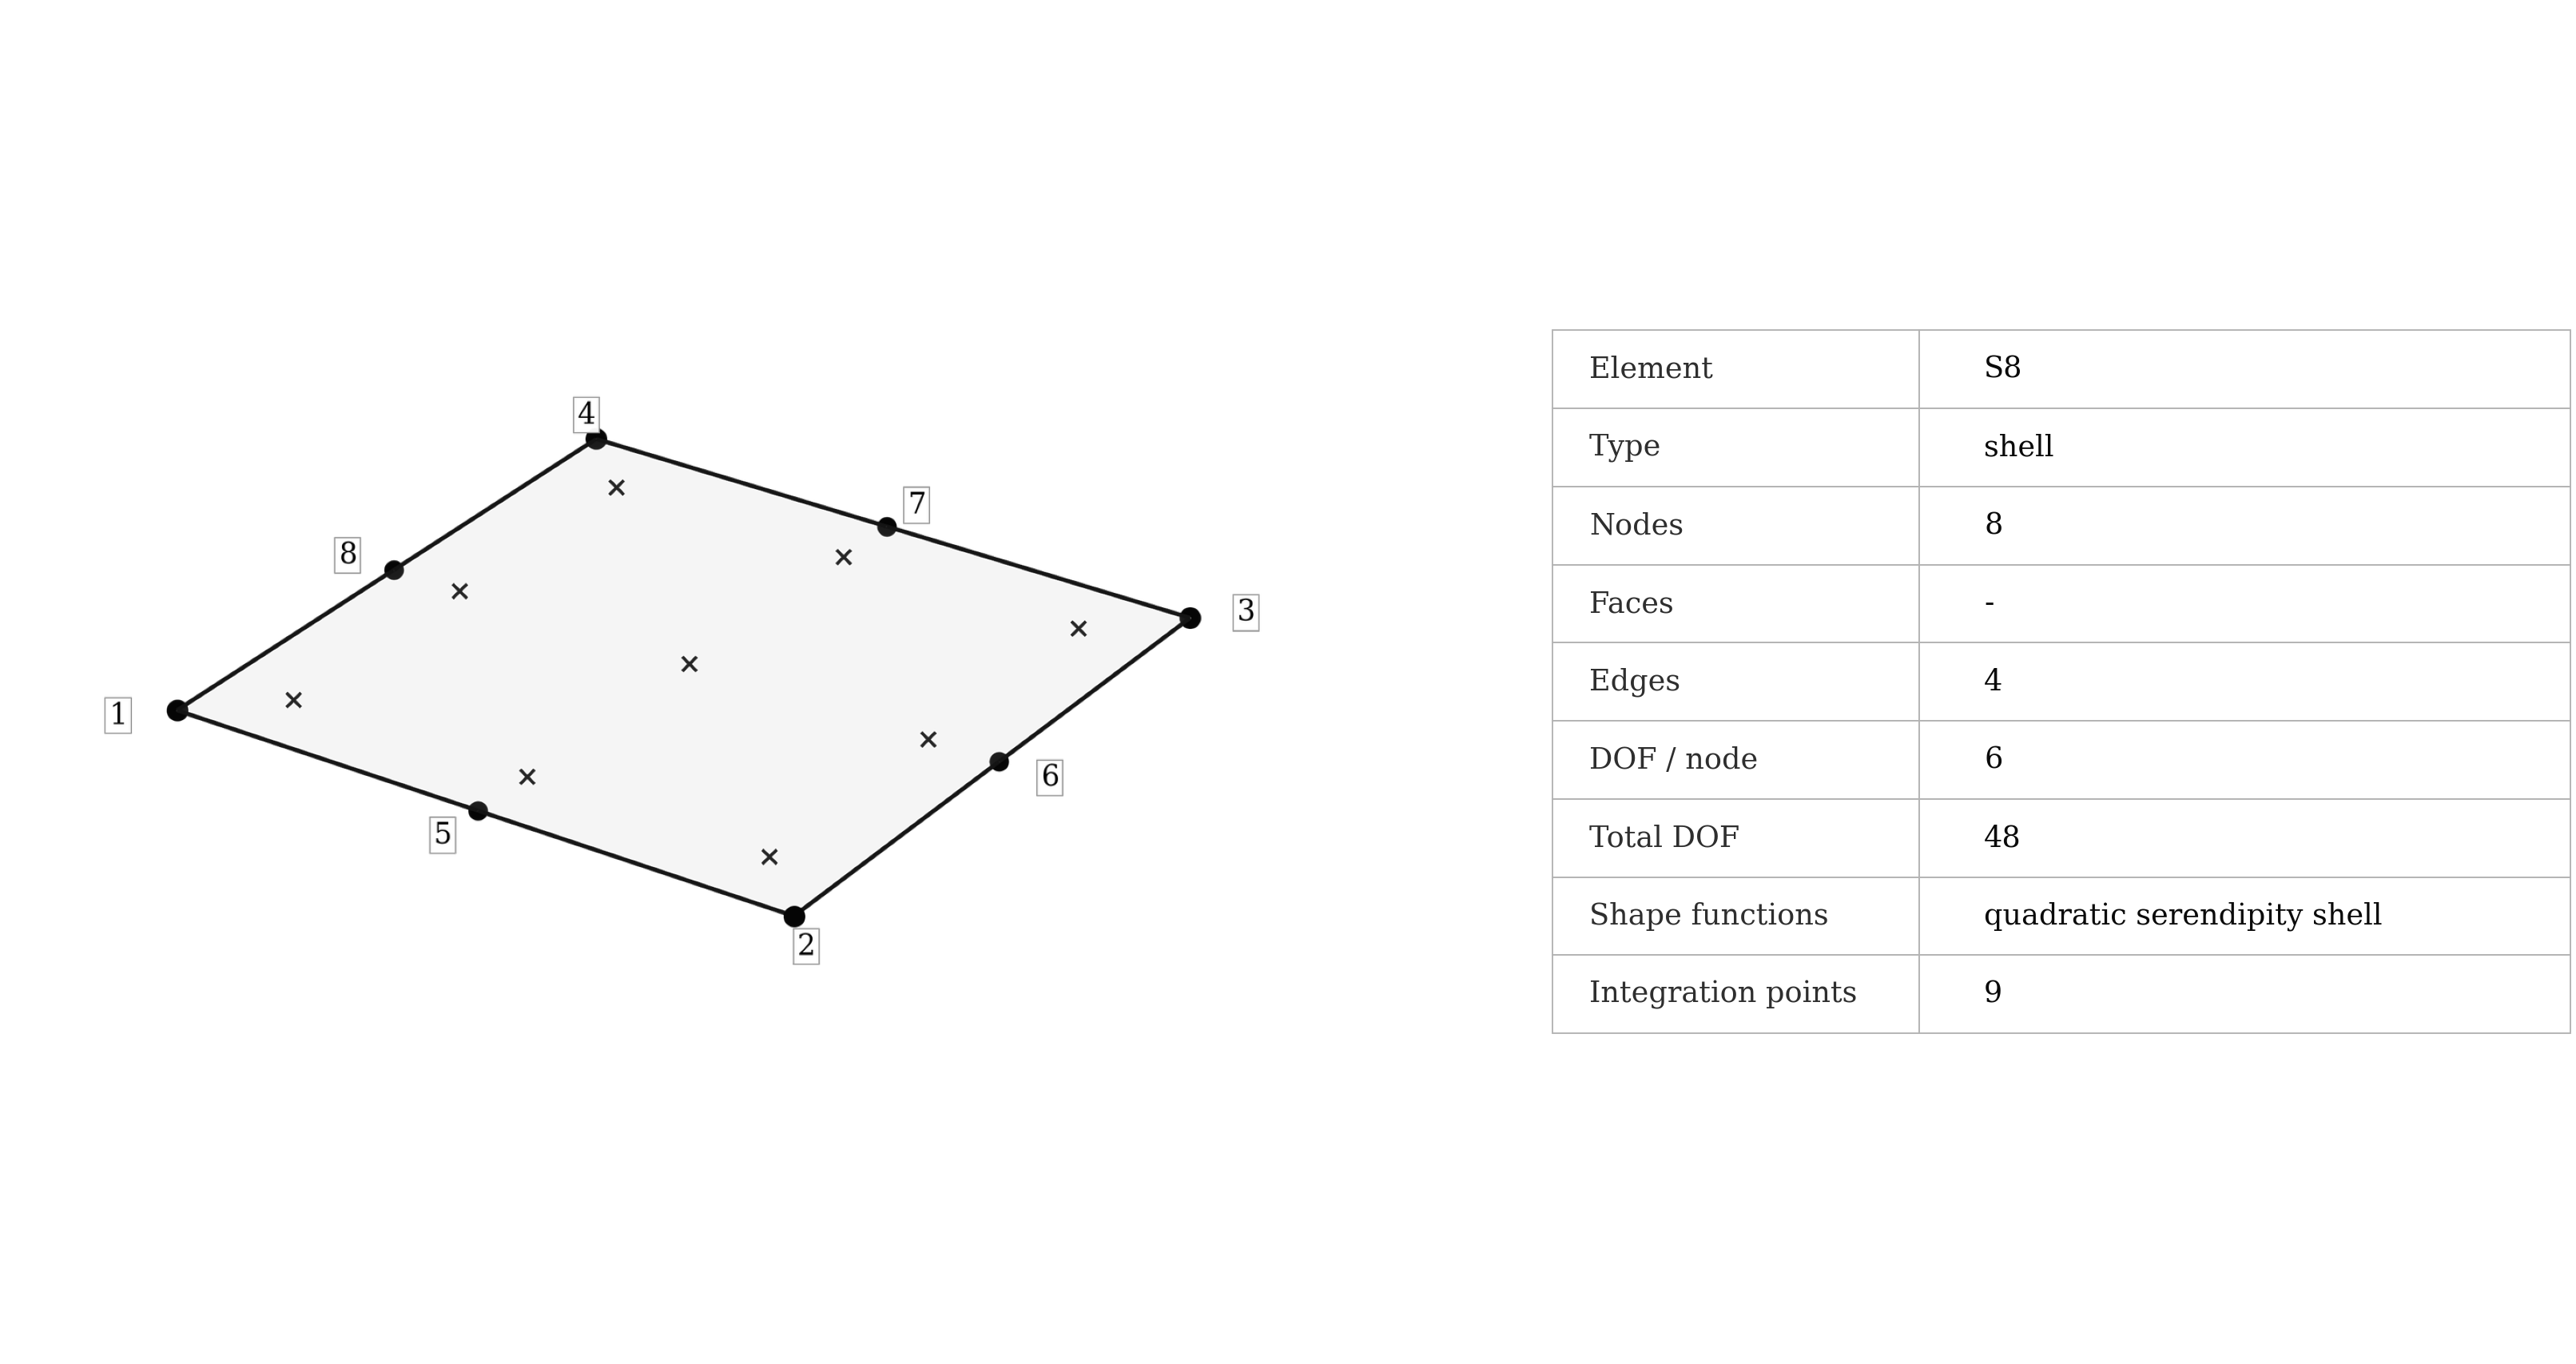
\includegraphics[width=0.80\linewidth]{pages/figures/element_schematics/s8_schematic.png}
    \caption{\val{S8} quadratic quadrilateral shell.}
\end{figure}

\begin{syntax}
*ELEMENT, TYPE=S8, ELSET=<set>
<id>, <n1>, <n2>, <n3>, <n4>, <n5>, <n6>, <n7>, <n8>
\end{syntax}

Native \val{S8} is the legacy eight-node quadratic quadrilateral shell. Four corner nodes and four midside nodes provide a higher-order surface interpolation than \val{S4}. This gives substantially better representation of curved geometry and smooth bending fields when the element is well shaped.

The formulation remains available for older models and comparison studies. For new models, use \val{MITC8FRT}. Higher order does not remove the need for good midside-node placement, reasonable aspect ratio, and controlled warping.

\clearpage
\section{\val{MITC8}: legacy 8-node MITC shell}

\begin{figure}[H]
    \centering
    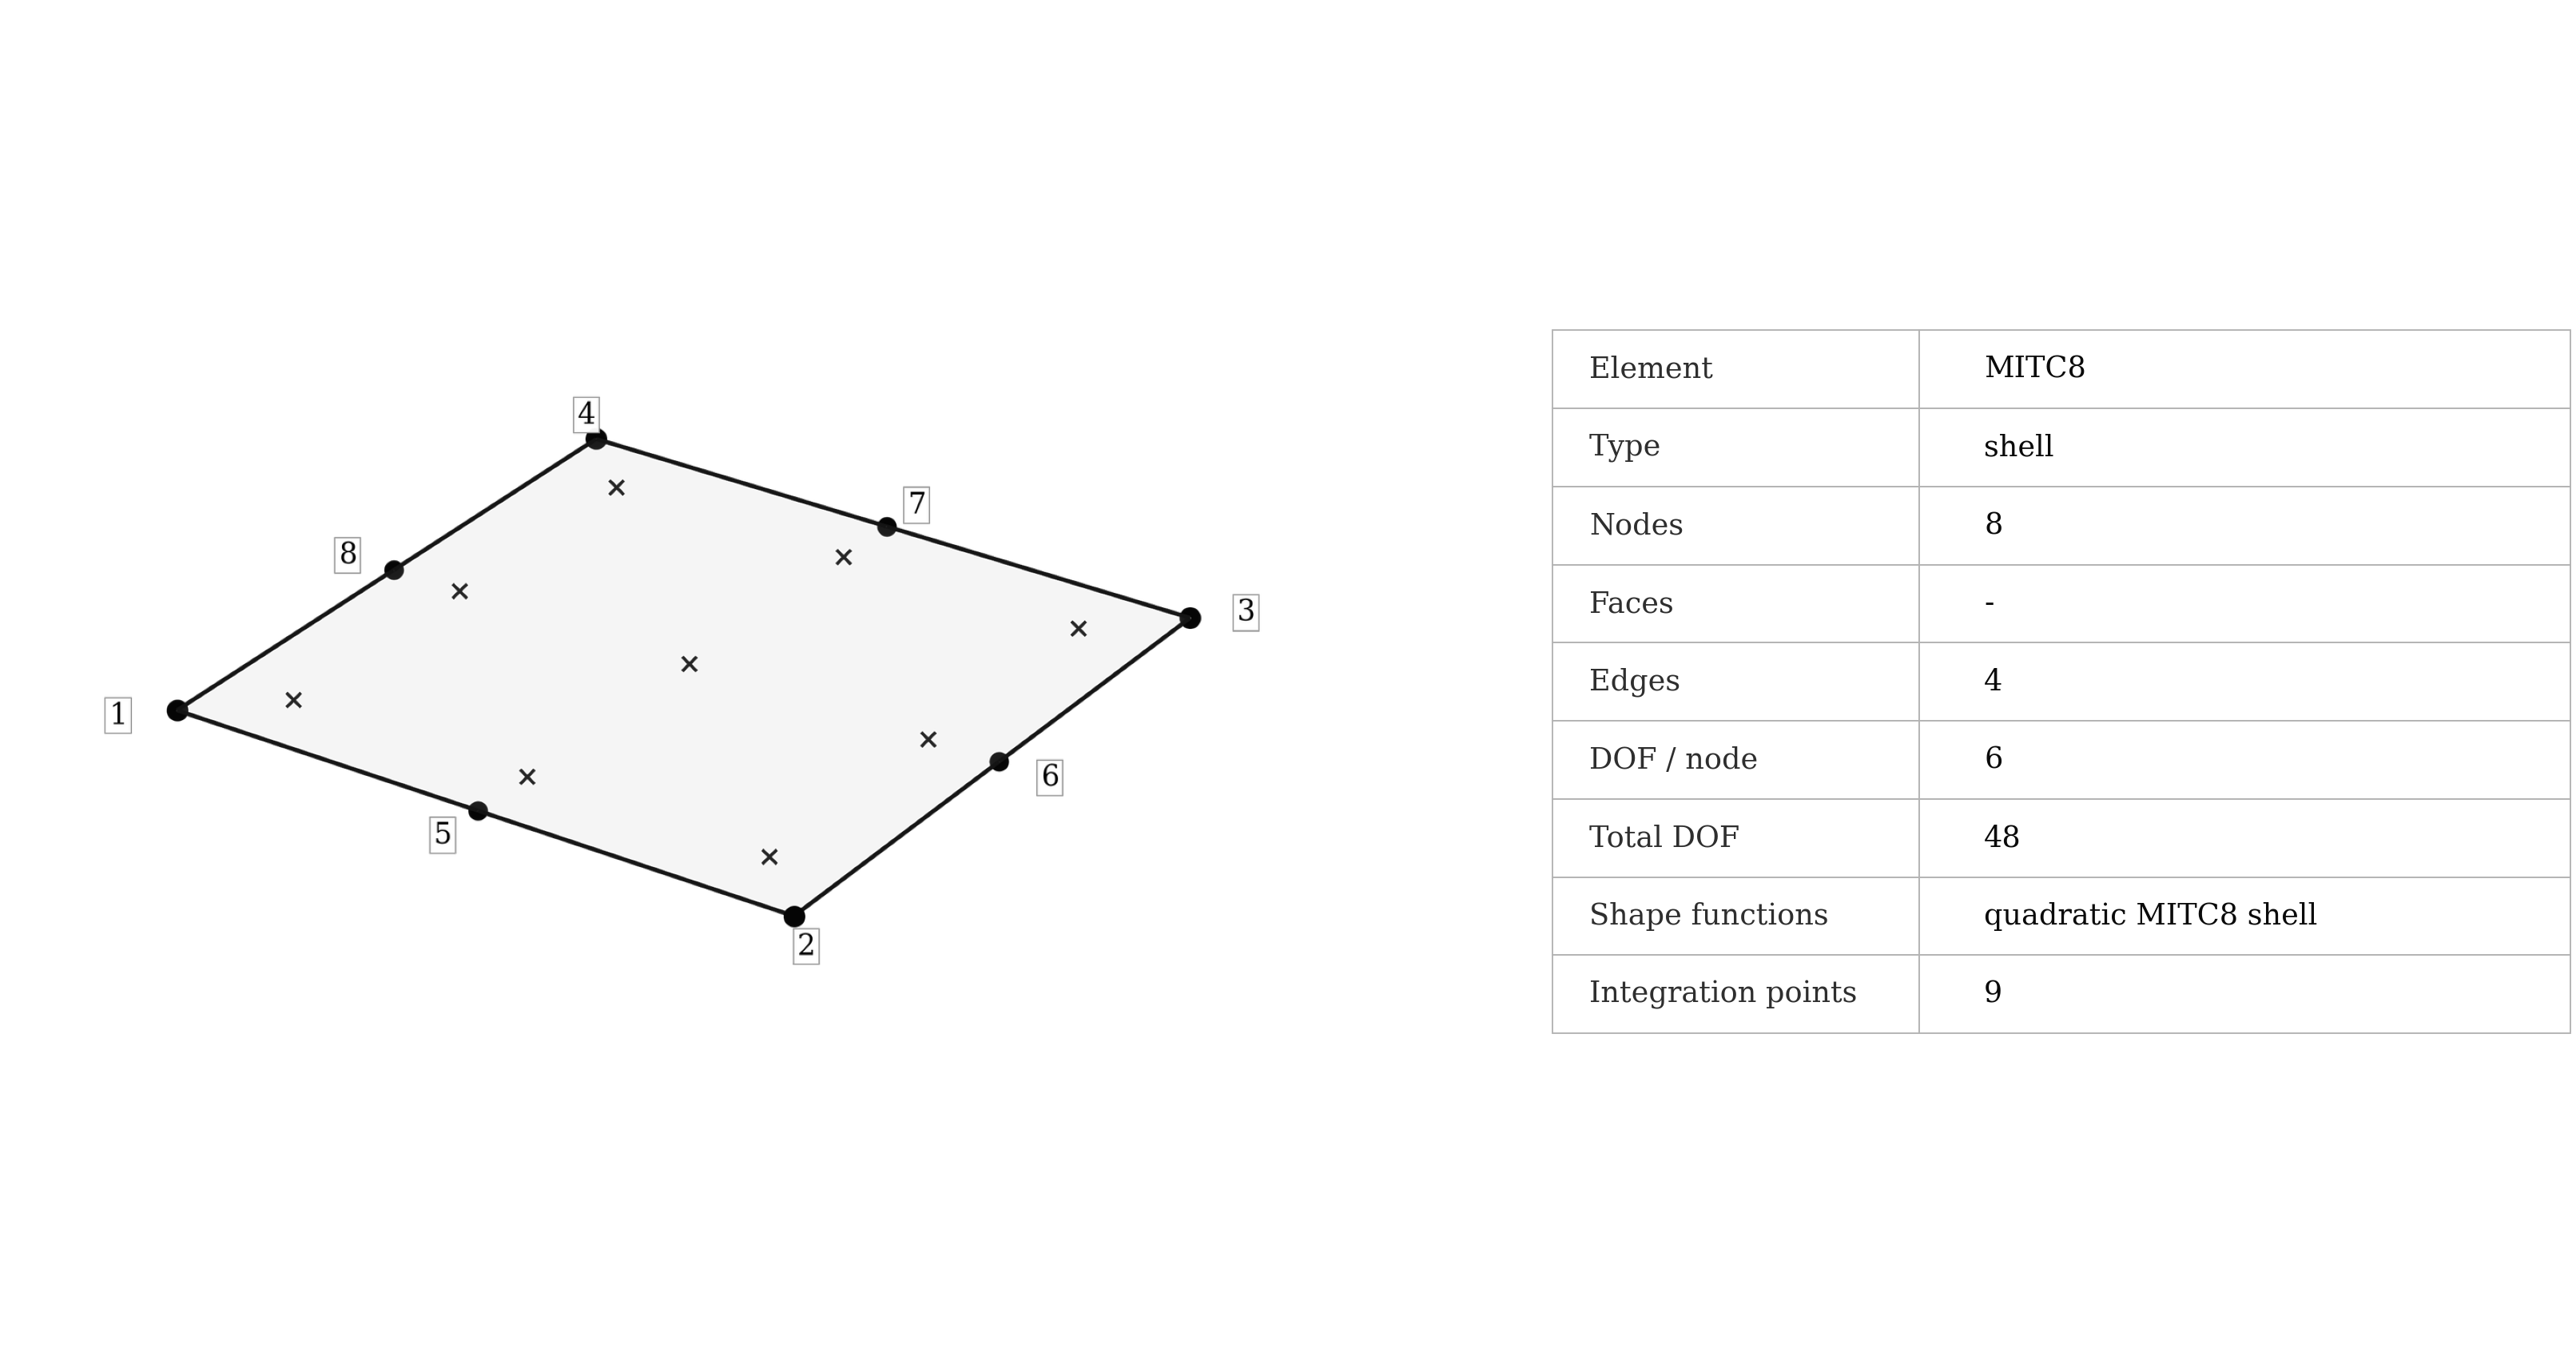
\includegraphics[width=0.80\linewidth]{pages/figures/element_schematics/mitc8_schematic.png}
    \caption{\val{MITC8} quadratic MITC shell.}
\end{figure}

\begin{syntax}
*ELEMENT, TYPE=MITC8, ELSET=<set>
<id>, <n1>, <n2>, <n3>, <n4>, <n5>, <n6>, <n7>, <n8>
\end{syntax}

\val{MITC8} combines the eight-node quadratic quadrilateral topology with MITC-style transverse-shear interpolation. It provides excellent thin-shell bending behaviour in the legacy linear shell family and is useful as a reference formulation for verifying lower-order shell results.

Because the interpolation is quadratic, a regular \val{MITC8} mesh can reproduce smooth bending fields with relatively few elements. The cost per element is higher than for \val{MITC4}, and distorted midside geometry can reduce the expected advantage.

For new nonlinear or general-purpose shell models, prefer \val{MITC8FRT}. Use native \val{MITC8} where comparison with legacy linear shell results is specifically required.

\clearpage
\section{\val{MITC8FRT}: finite-rotation 8-node MITC shell}

\begin{figure}[H]
    \centering
    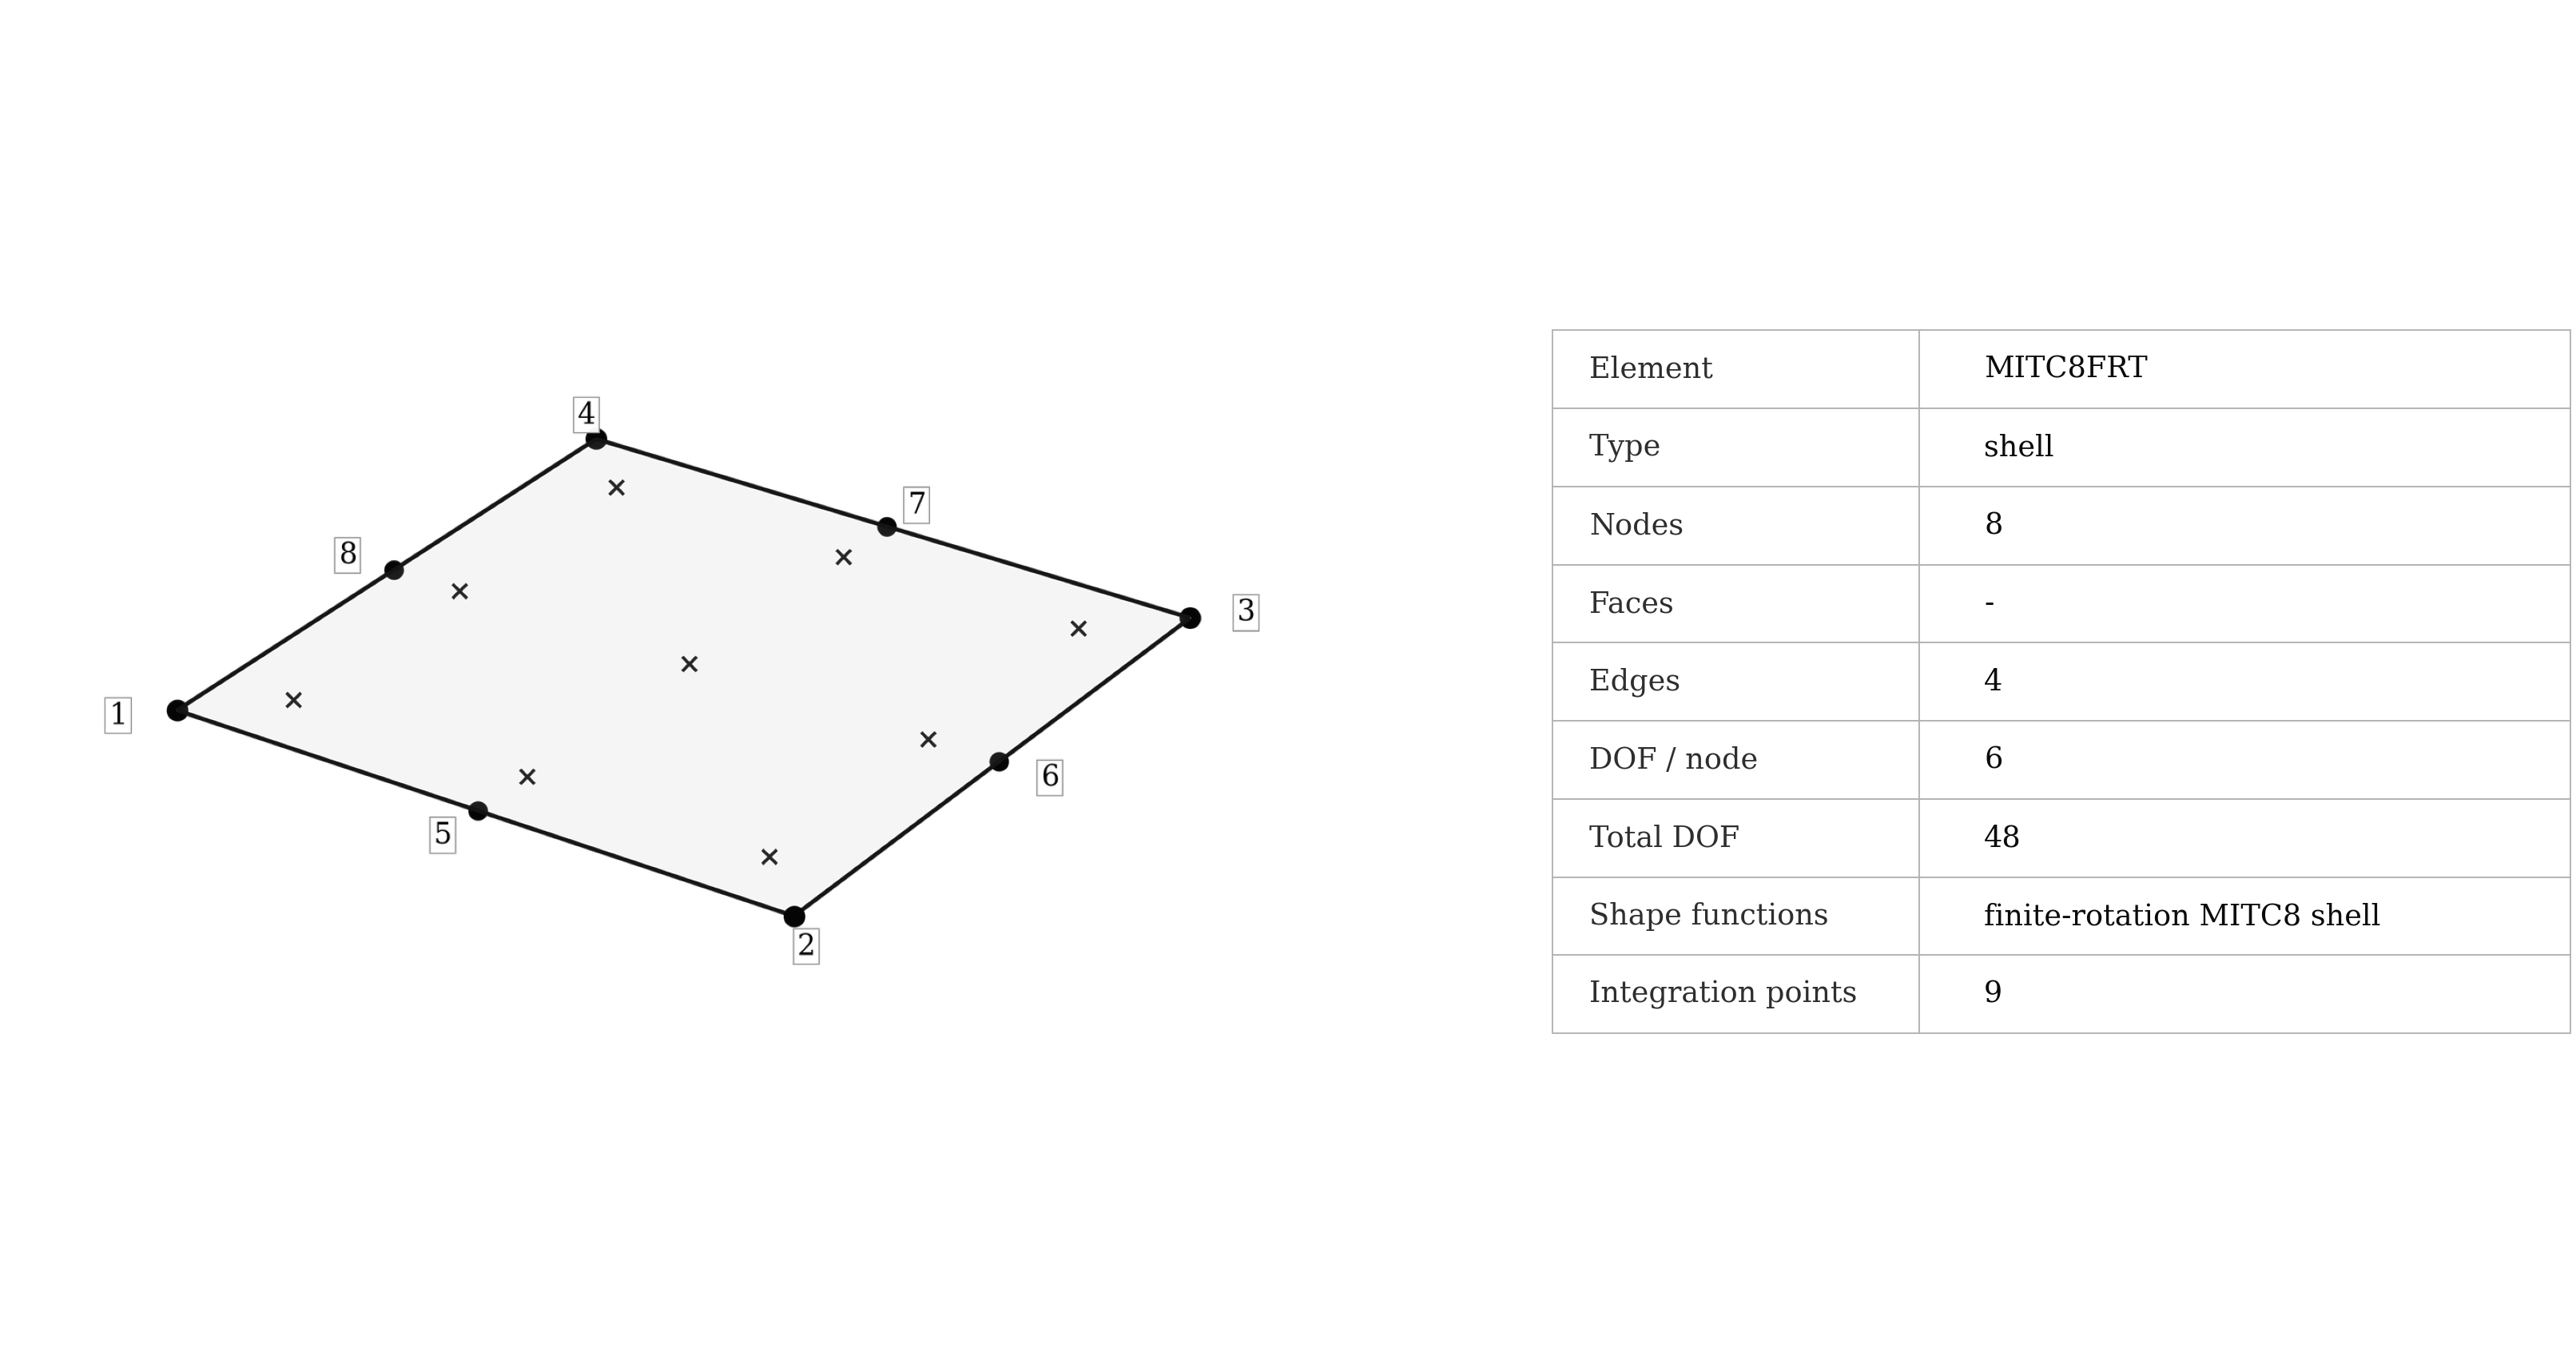
\includegraphics[width=0.80\linewidth]{pages/figures/element_schematics/mitc8frt_schematic.png}
    \caption{\val{MITC8FRT} finite-rotation eight-node shell.}
\end{figure}

\begin{syntax}
*ELEMENT, TYPE=MITC8FRT, ELSET=<set>
<id>, <n1>, <n2>, <n3>, <n4>, <n5>, <n6>, <n7>, <n8>
\end{syntax}

\val{MITC8FRT} is the recommended higher-order quadrilateral shell. It combines an eight-node midsurface interpolation with finite-rotation shell kinematics and MITC transverse-shear treatment. It is intended for accurate bending and curved-shell modelling where the additional interpolation order is worth the increased element cost.

The formulation is especially useful when a curved shell geometry can be represented with a clean quadratic quadrilateral mesh. Compared with a low-order shell, fewer elements may be required to describe smooth curvature and stress-resultant gradients.

Higher order does not make the formulation insensitive to distortion. Warped quadrilaterals, poorly placed midside nodes, inconsistent normals, and abrupt mesh transitions can still produce misleading stiffness and result recovery. Large-rotation models should be checked with deformation-shape inspection and mesh refinement.

Both Abaqus \val{S8} and \val{S8R} are translated to \val{MITC8FRT}.

\clearpage
\section{\val{QSPT}: quadrilateral shear-panel element}

\begin{figure}[H]
    \centering
    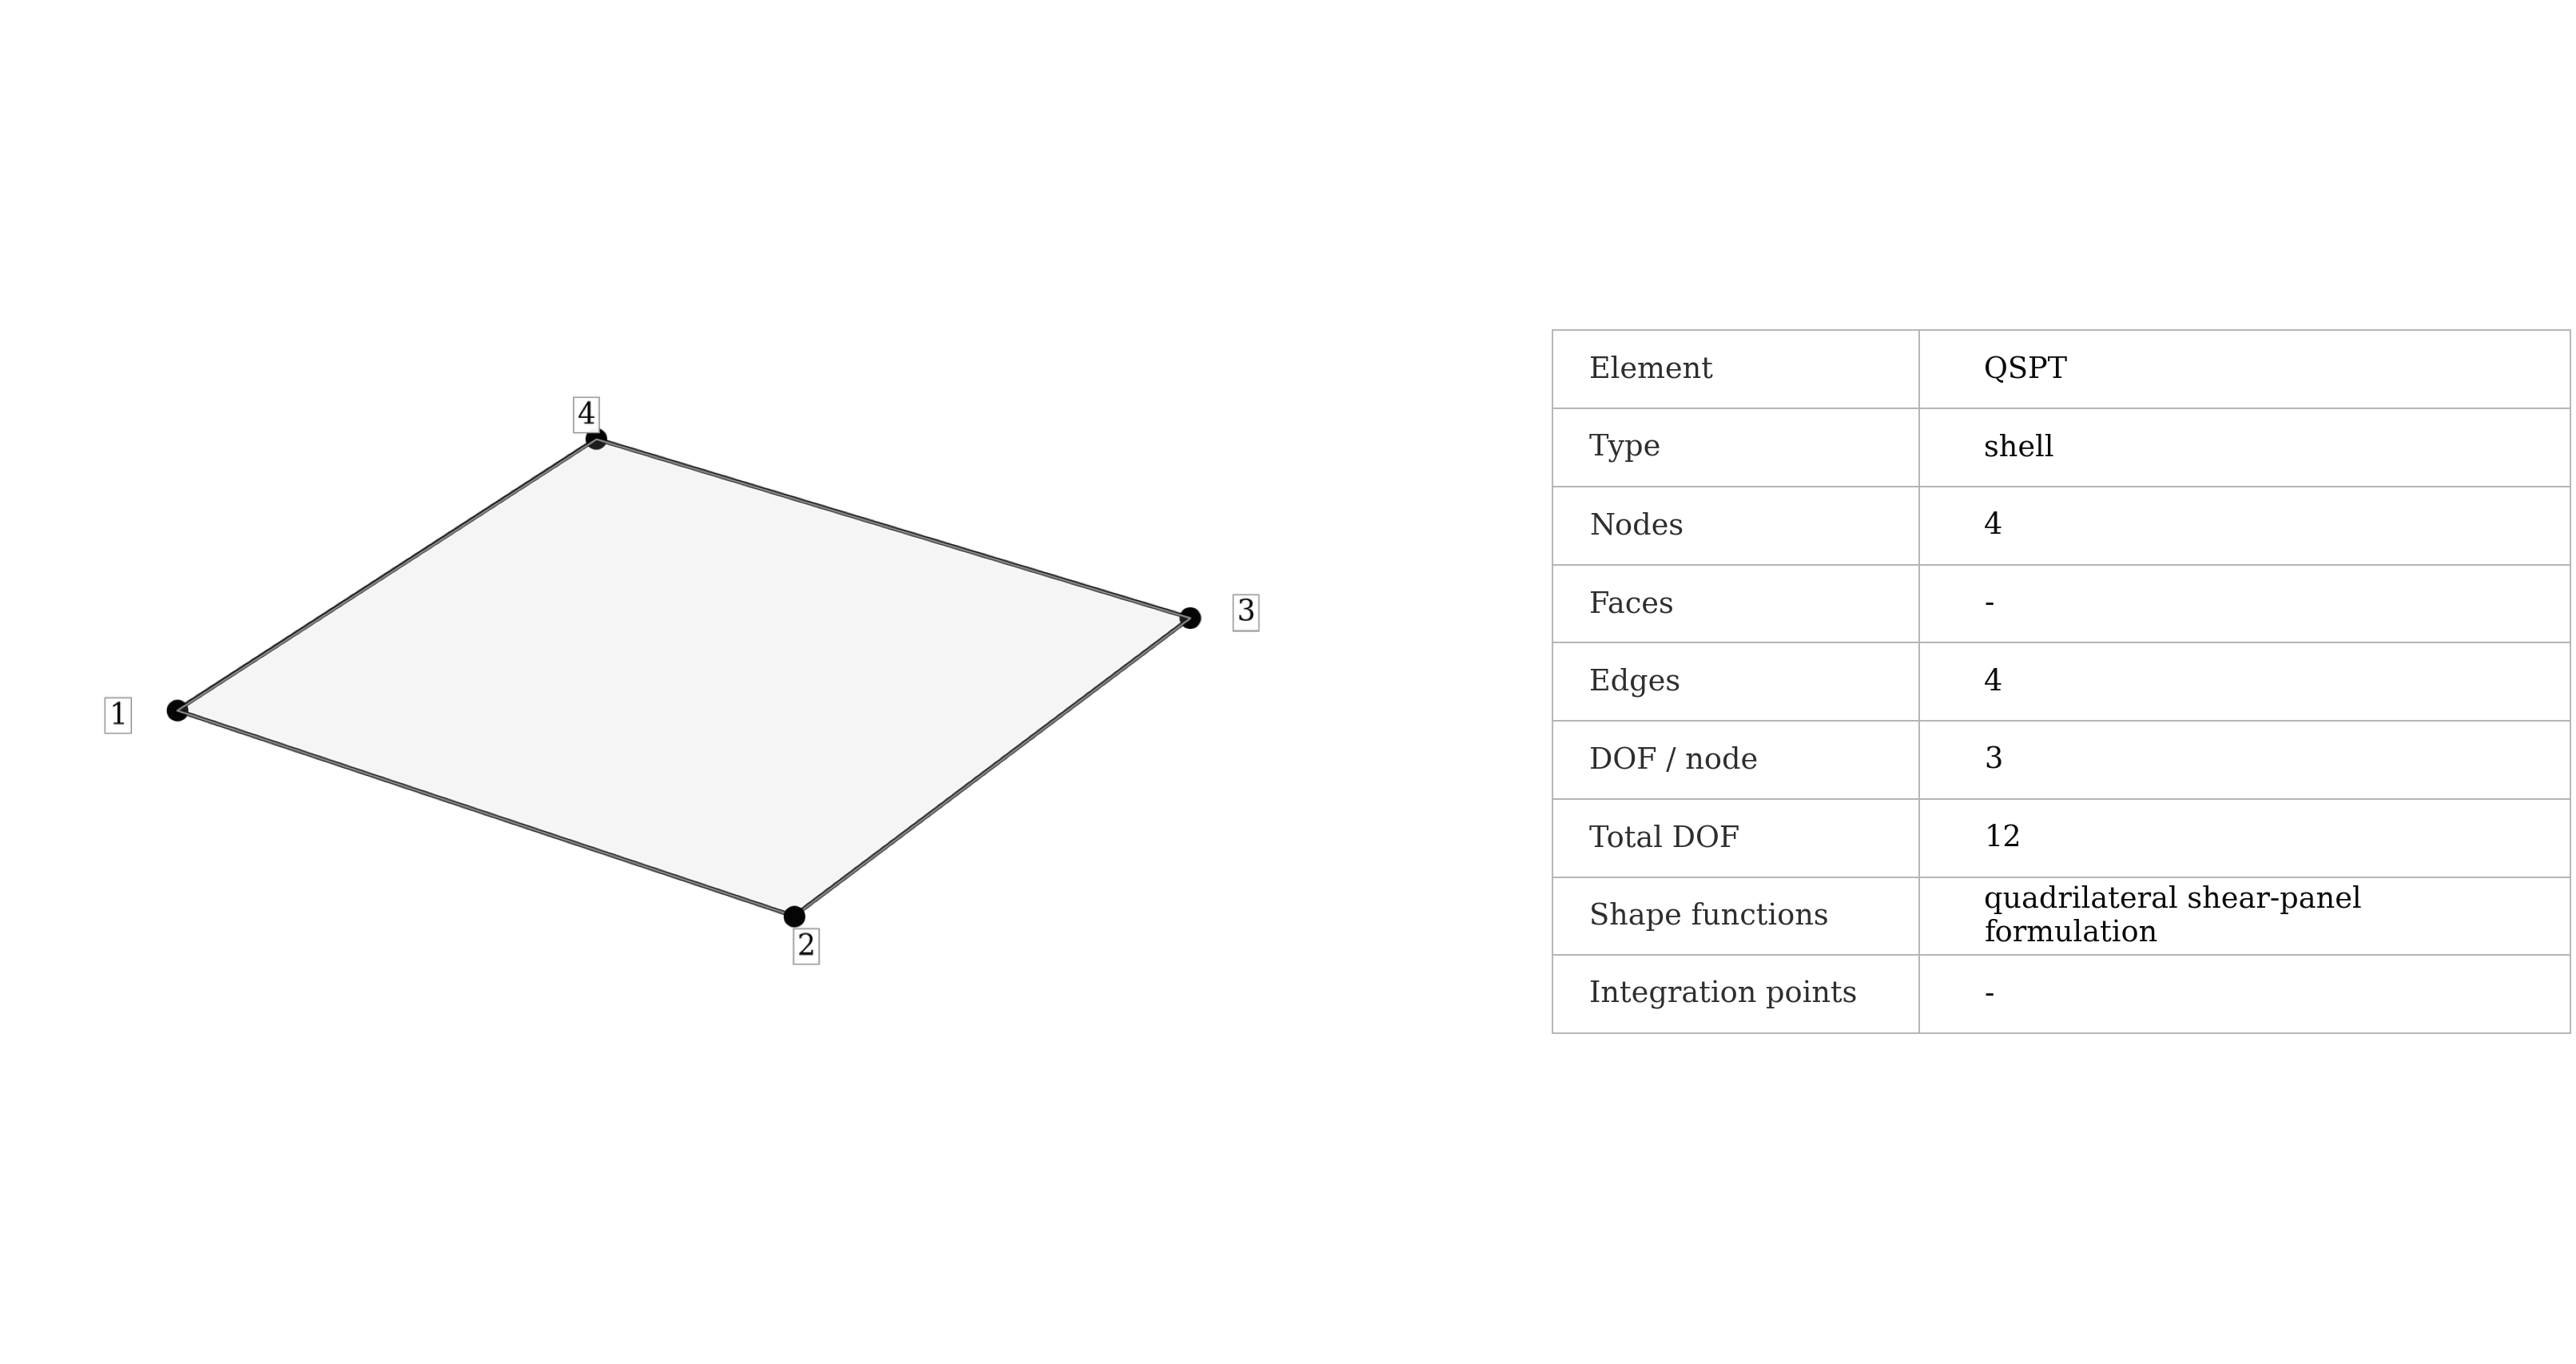
\includegraphics[width=0.78\linewidth]{pages/figures/element_schematics/qspt_schematic.png}
    \caption{\val{QSPT} shear-panel element.}
\end{figure}

\begin{syntax}
*ELEMENT, TYPE=QSPT, ELSET=<set>
<id>, <n1>, <n2>, <n3>, <n4>
\end{syntax}

\val{QSPT} is a specialized four-node quadrilateral panel element developed for shear-flow-oriented structural idealizations. It is intended for simplified panel models where the principal purpose of the element is to transfer in-plane shear rather than reproduce the complete behaviour of a general shell.

Typical applications are preliminary thin-walled structures, webs, aircraft-style shear panels, and reduced-order structural models in which panel shear flow is the primary quantity of interest. In such models \val{QSPT} can provide a compact load-path representation without introducing a complete shell formulation for every panel.

Do not use \val{QSPT} merely because the mesh contains four-node quadrilaterals. It is not a general replacement for \val{MITC4FRT}. If bending stiffness, local shell curvature, full shell resultants, or detailed top/bottom stresses are required, use a shell formulation instead.

\section{Beam and truss elements}

Line elements idealize slender three-dimensional members by describing the cross-section through section properties instead of meshing it explicitly. This can reduce the number of degrees of freedom by orders of magnitude compared with shell or solid modelling. The trade-off is that local three-dimensional connection behaviour, detailed cross-section distortion, holes, welds, and local stress concentrations are not resolved.

\clearpage
\section{\val{B33}: 3D beam element}

\begin{figure}[H]
    \centering
    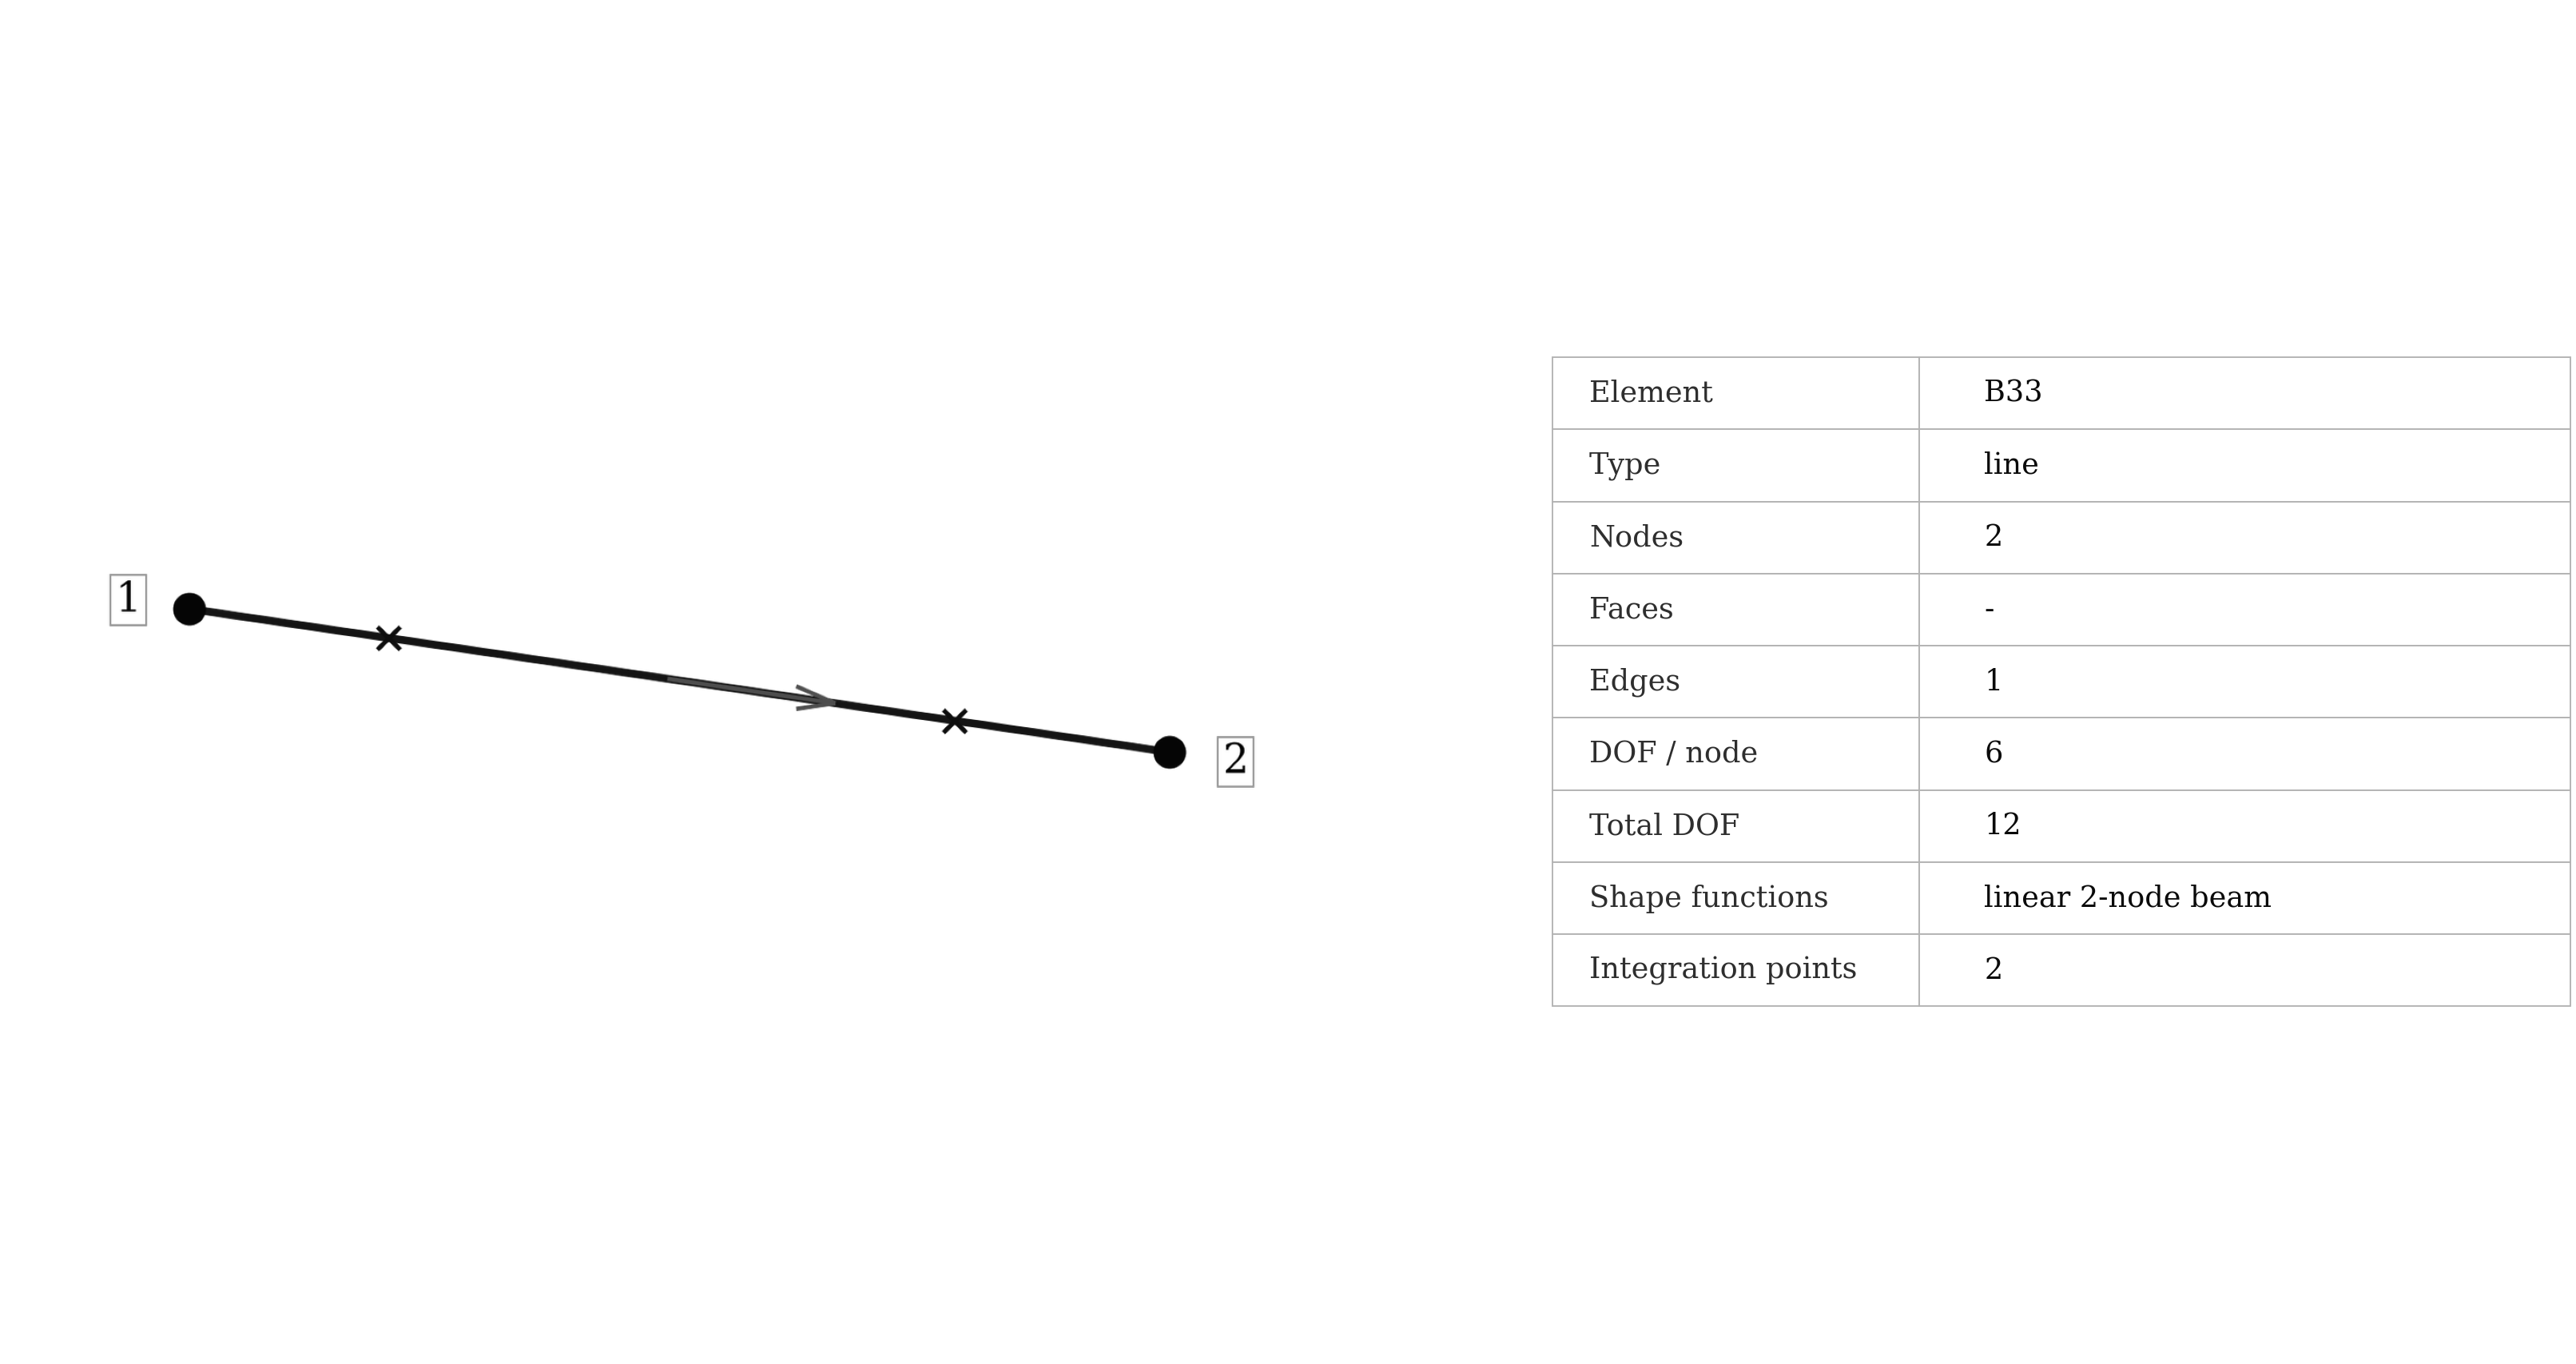
\includegraphics[width=0.70\linewidth]{pages/figures/element_schematics/b33_schematic.png}
    \caption{\val{B33} beam element.}
\end{figure}

\begin{syntax}
*ELEMENT, TYPE=B33, ELSET=<set>
<id>, <n1>, <n2>
\end{syntax}

\val{B33} is a two-node three-dimensional beam element with translational and rotational nodal degrees of freedom. It represents axial deformation, bending, torsion, and the section response defined by \cmd{BEAM SECTION} and the referenced \cmd{PROFILE}.

The current \cmd{ELEMENT} syntax uses exactly two connectivity nodes for \val{B33}. Beam cross-section orientation is supplied by the orientation vector in \cmd{BEAM SECTION}; an additional orientation node is not part of the current connectivity grammar.

Beam elements are appropriate for slender frames, stiffeners, spars, ribs, idealized support members, and other structures where section forces and global deformation are the main engineering quantities. They permit axial area, bending inertias, torsional stiffness, product of inertia, section offsets, and reference-line offsets to be represented without meshing the full cross-section.

The beam idealization does not resolve local connection stresses, bolt or weld geometry, detailed cross-section deformation, or three-dimensional load introduction. Use shells or solids when those local effects determine the design result. Always verify the beam local axes because bending moments, section forces, and profile properties are interpreted in that local system.

The supported Abaqus reader accepts \val{B33} with the same two-node connectivity.

\clearpage
\section{\val{T3}: 2-node truss element}

\begin{figure}[H]
    \centering
    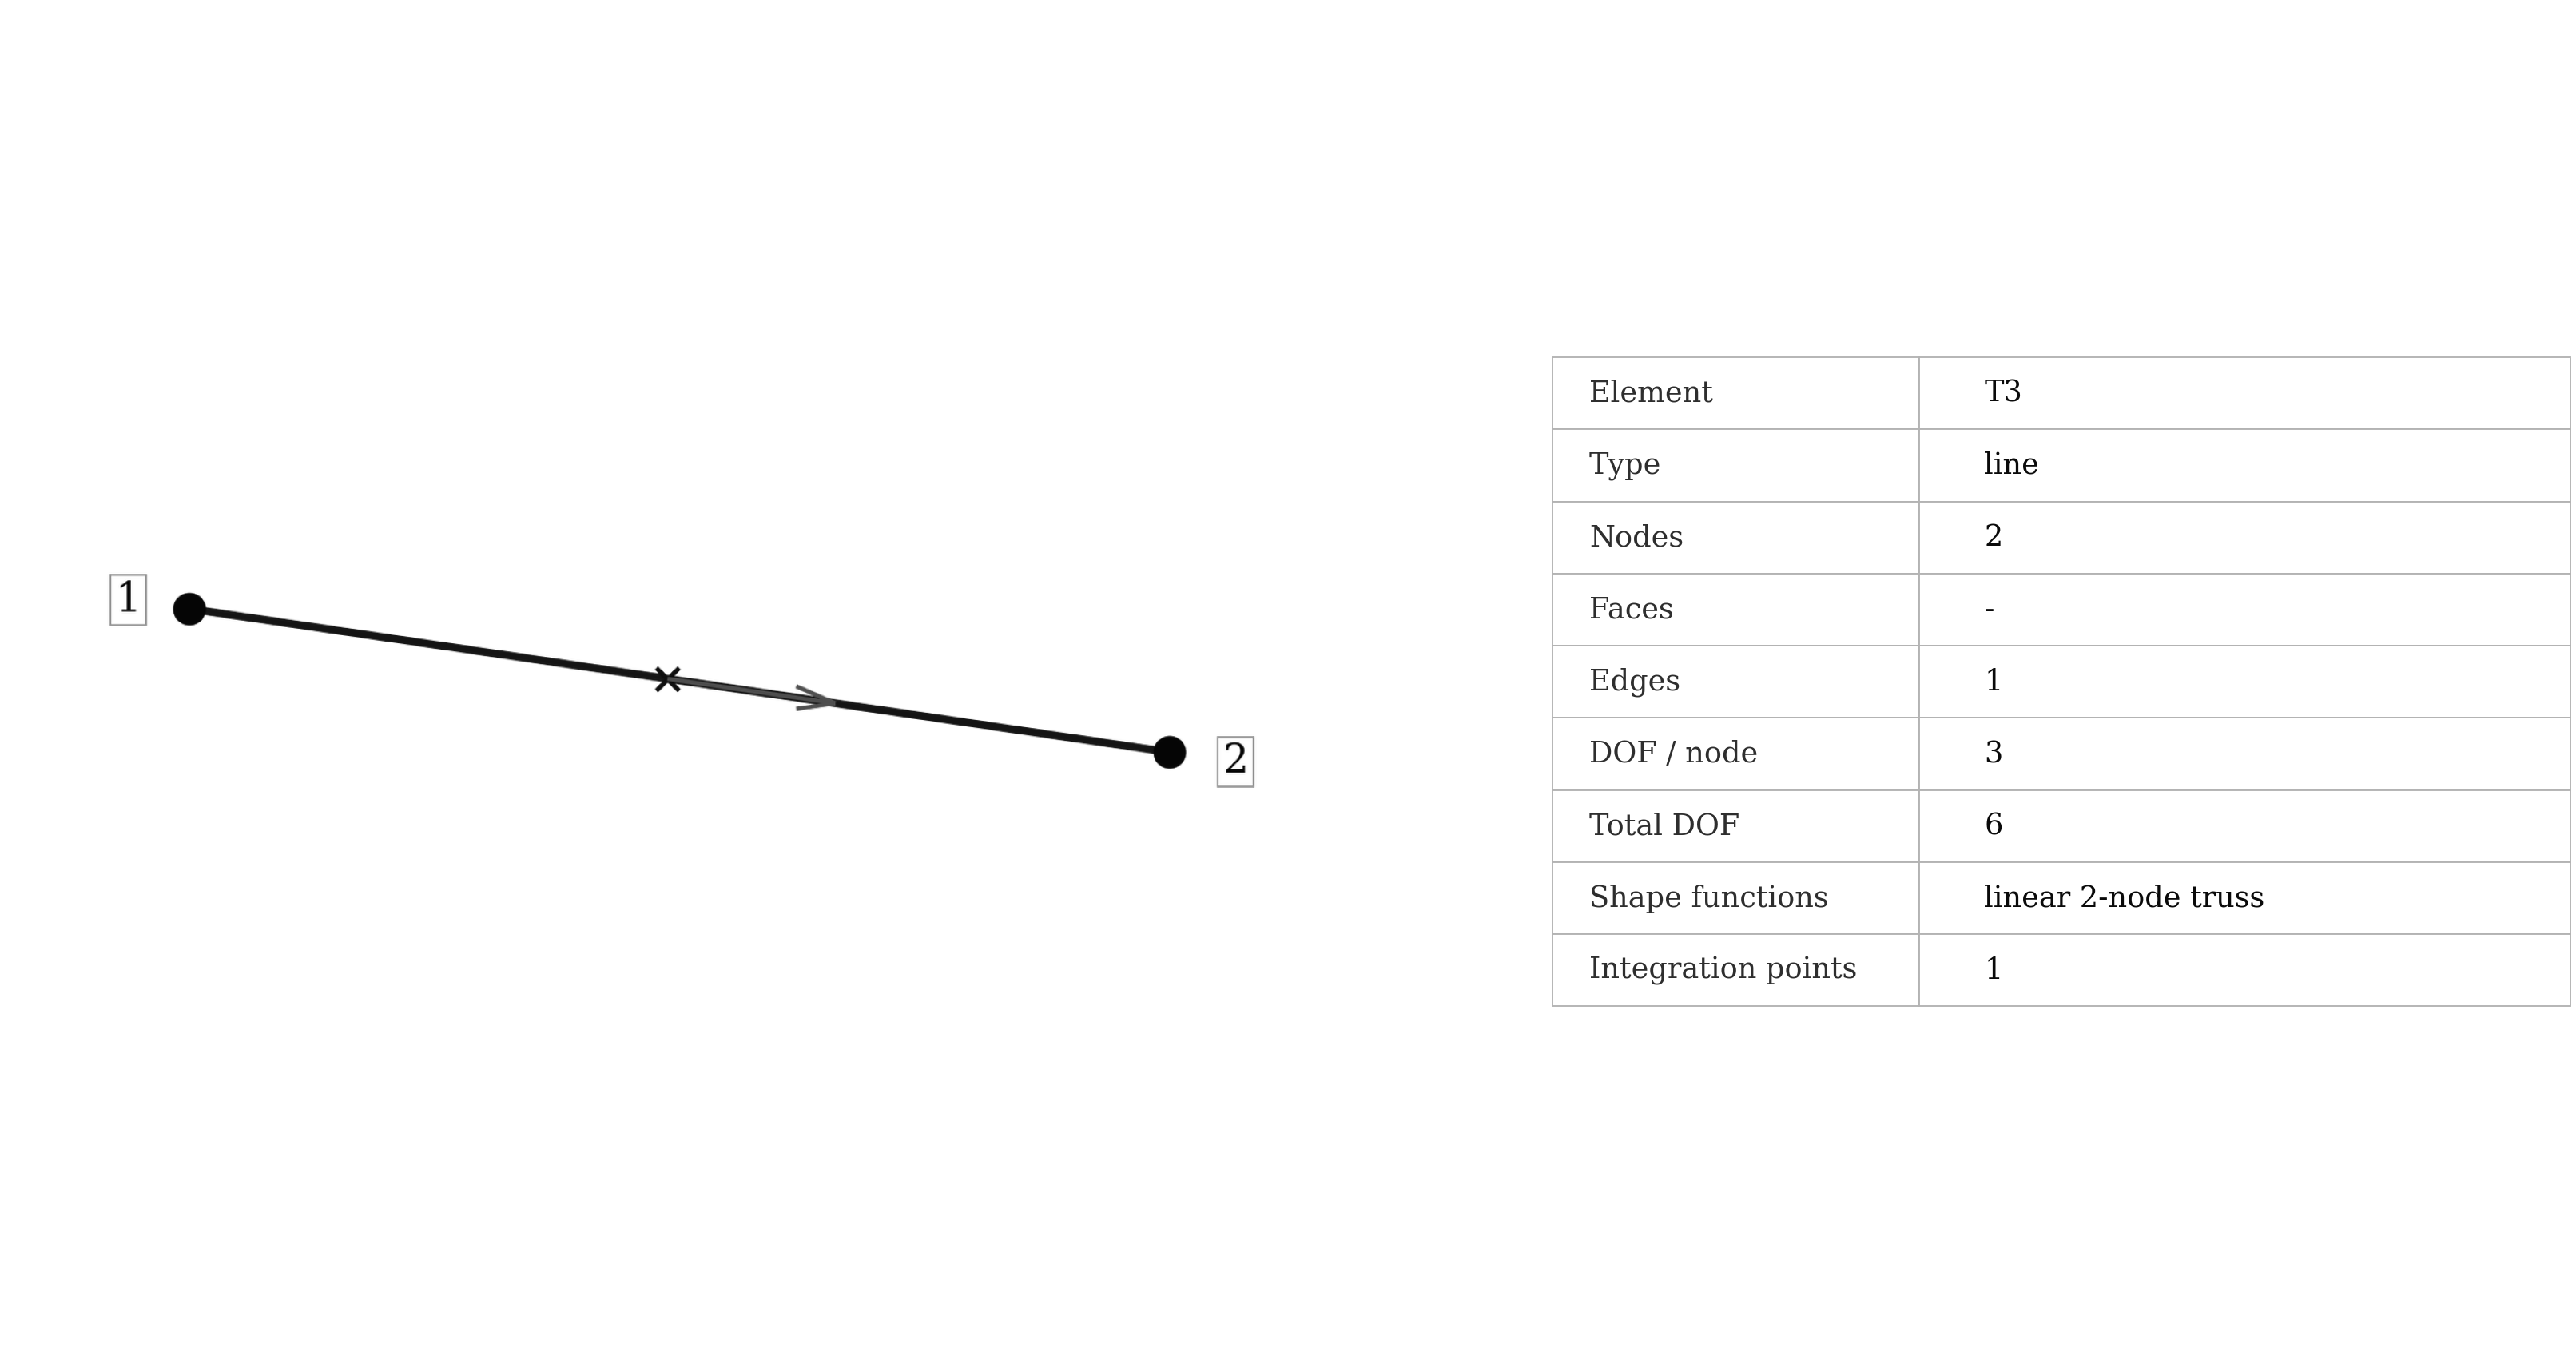
\includegraphics[width=0.68\linewidth]{pages/figures/element_schematics/t3_schematic.png}
    \caption{\val{T3} truss element.}
\end{figure}

\begin{syntax}
*ELEMENT, TYPE=T3, ELSET=<set>
<id>, <n1>, <n2>
\end{syntax}

\val{T3} is a two-node truss element. It carries axial force along its current line direction and uses translational nodal degrees of freedom. The material and cross-sectional area are assigned by \cmd{TRUSS SECTION}.

The element is appropriate for pin-jointed members, rods, braces, links, and other components whose intended structural action is axial tension or compression. Truss models are inexpensive and easy to interpret because the principal mechanical quantities are axial force, axial strain, and axial stress.

The limitations are deliberate. \val{T3} has no bending stiffness, no torsional stiffness, and no rotational continuity. It cannot model fixed-end moments, eccentric frame action, or transverse stiffness of a physical beam. If a member is expected to carry moment, use \val{B33} or a shell/solid representation.

In Abaqus input the corresponding accepted type is \val{T3D2}. The two labels select the same FEMaster truss formulation through their respective input dialects.

\section{Element selection guidelines}

No element is universally best. The following rules are useful starting points:
\begin{itemize}
  \item use \val{C3D10} rather than \val{C3D4} when tetrahedral stress accuracy matters;
  \item use well-shaped hexahedra when the geometry can be meshed naturally in a structured or swept way;
  \item treat \val{C3D5} as a transition element rather than the preferred bulk discretization;
  \item assess reduced-integration solids by deformation shape and refinement, not only by solver convergence;
  \item use the FRT shell family for new shell models, especially when finite rotations or nonlinear analysis are relevant;
  \item choose shell rather than solid idealization when through-thickness stress is not required and the structure is geometrically thin;
  \item choose beam or truss idealizations only when their one-dimensional kinematic assumptions match the physical member;
  \item verify reactions, deformed shapes, energy trends, and mesh convergence whenever the element choice materially affects the result.
\end{itemize}

A solver can converge accurately to the discrete equations of a poor finite-element model. Element selection and mesh convergence therefore remain modelling responsibilities rather than numerical post-processing details.

\chapter{Regions and Selections}
\label{chap:regions}

Regions give names to reusable parts of the mesh. They are used throughout a FEMaster model: Sections are assigned to element sets, supports and concentrated loads target nodes or node sets, pressure and traction loads act on surfaces, and constraints such as couplings, ties, and contact refer to named regions.

A region should therefore represent a meaningful modelling concept rather than only a convenient list of IDs. Names such as \val{ROOT}, \val{PRESSURE_FACE}, \val{DESIGN_DOMAIN}, or \val{CONTACT_SLAVE} make the intent of later commands much clearer than repeating numerical identifiers throughout the deck.

Regions can be defined inside a Part or at Assembly level. A Part-level region belongs to that Part and is available for every Instance of the Part. An Assembly-level region refers to the placed model and is useful when a selection belongs to one particular Instance or combines entities from several Instances. The optional \key{INSTANCE} parameter identifies the Instance whose local IDs are being referenced.

User node, element, and explicit surface IDs are non-negative labels and may start at \val{0}. Generated ranges therefore may also begin at zero.

\keywordpage{NSET}

\cmd{NSET} creates or extends a named node set. The same basic syntax is accepted by native FEMaster and by the supported Abaqus input format. \key{NSET} gives the set name; \key{NAME} is accepted as an alternative spelling. Data may contain explicit node references or generated arithmetic ranges.

Inside a Part, numerical entries refer to that Part's local node IDs. Separate Parts may therefore contain sets with the same numerical members without referring to the same physical nodes. If a Part is instantiated more than once, its Part-level node sets remain available for every copy.

At Assembly level, \key{INSTANCE=<name>} qualifies local IDs with one particular Instance. This is the most direct way to create a support or load region on one placed copy of a reusable Part. Assembly-level sets may also combine selections from different Instances by using the supported qualified references or by building larger sets from previously named regions.

With \key{GENERATE}, every data row contains
\[
\text{start},\quad \text{end},\quad \text{increment}.
\]
The end value is inclusive. The increment defaults to 1 and must not be zero. Positive and negative increments are supported, so generated sequences can run in either direction as long as the sign agrees with the requested range.

\begin{keywordparameters}
\key{NSET} / \key{NAME} & required & Name of the node set to create or extend. \\
\key{INSTANCE} & optional & Assembly-level qualifier for local node references. \\
\key{GENERATE} & optional flag & Interpret each data row as start, end, increment. \\
\end{keywordparameters}

\begin{keyworddata}
Explicit form & One or more node IDs or supported named/qualified node references. \\
Generated form & \val{start, end, increment}; the increment defaults to \val{1} and must be nonzero. \\
\end{keyworddata}

\exampleheading

\begin{dialectexamples}
\begin{femasterdeck}
*PART, NAME=BEAM
*NODE
0, 0., 0., 0.
1, 1., 0., 0.
2, 2., 0., 0.
3, 3., 0., 0.
*NSET, NSET=ENDS
0, 3
*NSET, NSET=ALLN, GENERATE
0, 3, 1
*END PART
\end{femasterdeck}
\begin{abaqusdeck}
*PART, NAME=BEAM
*NODE
0, 0., 0., 0.
1, 1., 0., 0.
2, 2., 0., 0.
3, 3., 0., 0.
*NSET, NSET=ENDS
0, 3
*NSET, NSET=ALLN, GENERATE
0, 3, 1
*END PART
\end{abaqusdeck}
\end{dialectexamples}

\notesheading

Prefer Part-level sets for regions that are intrinsic to the component, such as a bolt row, a root edge, or a material domain. Prefer Assembly-level sets for selections whose meaning depends on placement, such as ``the left support of Instance A'' or a region combining nodes from several components.

\clearpage
\subsection*{Assembly-level Instance selection}

A typical Assembly selection looks like
\begin{syntax}
*ASSEMBLY
*INSTANCE, NAME=BEAM_A, PART=BEAM
0., 0., 0.
*END INSTANCE
*INSTANCE, NAME=BEAM_B, PART=BEAM
100., 0., 0.
*END INSTANCE

*NSET, NSET=SUPPORT_A, INSTANCE=BEAM_A
0
*NSET, NSET=SUPPORT_B, INSTANCE=BEAM_B
0
*END ASSEMBLY
\end{syntax}
Both sets contain a local node with ID \val{0}, but they refer to different placed Instances.

\keywordpage{ELSET}

\cmd{ELSET} is the element-domain counterpart of \cmd{NSET}. It creates or extends a named element set from explicit element references or generated ranges. \key{ELSET} supplies the name and \key{NAME} is accepted as an alternative.

Element sets are central to property assignment. Solid, shell, beam, and truss Sections normally target an \cmd{ELSET}, so a good element-set structure often mirrors the physical construction of the model: different materials, thicknesses, beam profiles, or design domains should have separate meaningful names.

Inside a Part, entries refer to that Part's local element IDs. At Assembly level, \key{INSTANCE} qualifies local IDs with one placed Instance. This allows two Instances of the same Part to be selected independently even though they use identical local element numbering.

\key{GENERATE} follows the same inclusive start/end/increment rule as \cmd{NSET}. ID \val{0} is valid, so for example \val{0, 99, 1} generates one hundred element IDs if they exist in the intended topology.

\begin{keywordparameters}
\key{ELSET} / \key{NAME} & required & Name of the element set to create or extend. \\
\key{INSTANCE} & optional & Assembly-level qualifier for local element references. \\
\key{GENERATE} & optional flag & Generate an arithmetic sequence of element IDs. \\
\end{keywordparameters}

\begin{keyworddata}
Explicit form & One or more element IDs or supported named/qualified element references. \\
Generated form & \val{start, end, increment}; inclusive end, nonzero increment. \\
\end{keyworddata}

\exampleheading

\begin{dialectexamples}
\begin{femasterdeck}
*ELSET, ELSET=DESIGN_DOMAIN, GENERATE
0, 99, 1

*ELSET, ELSET=EVEN_ELEMENTS, GENERATE
0, 98, 2
\end{femasterdeck}
\begin{abaqusdeck}
*ELSET, ELSET=DESIGN_DOMAIN, GENERATE
0, 99, 1

*ELSET, ELSET=EVEN_ELEMENTS, GENERATE
0, 98, 2
\end{abaqusdeck}
\end{dialectexamples}

\notesheading

A Section assigned to a Part-level element set belongs to that component and therefore follows every Instance of the Part. This is normally the desired behaviour for material and geometric properties. Assembly-level element sets are more useful for loads, diagnostics, or selections that depend on which copy of the Part is being addressed.

\keywordpage{SURFACE}

\cmd{SURFACE} defines a geometric boundary from element sides. A surface is more than a node set: it retains which element face is selected and therefore has a well-defined interpolation, area or line measure, and orientation. Surface information is required for pressure loads, distributed tractions, surface couplings, ties, and contact.

A side is selected by an element or element-set target together with a side label such as \val{S1}, \val{S2}, and so on. The actual face represented by a side label depends on the element type and its connectivity. This makes element node ordering important: reversing or changing connectivity can also change the physical direction of a surface normal.

For shell elements the two sides of the midsurface can also be described by \val{SPOS} and \val{SNEG}. These represent the positive and negative shell sides and are useful when pressure direction or top/bottom interpretation matters.

Native FEMaster additionally supports an explicit surface-ID form in which a user surface ID is supplied together with the parent element and side. Explicit surface IDs are non-negative and may start at \val{0}. For most user-written decks, however, naming a surface directly from an element or element set is clearer and avoids managing a separate numerical surface-ID space.

At Assembly level, \key{INSTANCE} can qualify the target element or element set. This allows a face of one particular Instance to be selected even when several copies use the same local element IDs and set names.

The Abaqus example uses the supported element-based \cmd{SURFACE, TYPE=ELEMENT} syntax. More specialized surface features available in the full Abaqus product should not be assumed to be accepted unless they are documented here.

\begin{keywordparameters}
\key{SFSET} / \key{NAME} & optional & Name of the destination surface region; native default \val{SFALL}. \\
\key{INSTANCE} & optional & Assembly-level Instance qualifier. \\
\end{keywordparameters}

\begin{keyworddata}
Target form & \val{element-or-elset, side}. \\
Explicit native form & \val{surface_id, element_id, side}. \\
\end{keyworddata}

\exampleheading

\begin{dialectexamples}
\begin{femasterdeck}
*SURFACE, NAME=TOP
SOLIDS, S2

*SURFACE, NAME=ONE_FACE
0, 42, S1
\end{femasterdeck}
\begin{abaqusdeck}
*SURFACE, NAME=TOP, TYPE=ELEMENT
SOLIDS, S2
\end{abaqusdeck}
\end{dialectexamples}

\notesheading

Do not infer a pressure or contact normal from an unordered node set. Define the correct element side and inspect the surface orientation. For shell models, normal consistency is especially important because it also controls positive/negative shell faces and the sign convention of bending-related quantities.

\keywordpage{SFSET}

\cmd{SFSET} groups existing native FEMaster surface entities into a named surface region. It is useful when surfaces have been created with explicit user surface IDs or when several previously defined surface groups should be combined into one target.

\cmd{SURFACE} and \cmd{SFSET} therefore serve different purposes: \cmd{SURFACE} creates geometric boundary entities from elements, while \cmd{SFSET} collects already existing surface entities. If the desired boundary can be expressed directly from one or more element sets, a named \cmd{SURFACE} is usually the simpler representation.

The destination name is supplied by \key{SFSET} or \key{NAME}; the native default is \val{SFALL}. Explicit surface references can be listed directly. With \key{GENERATE}, arithmetic ranges of surface IDs can be produced using the same inclusive start/end/increment convention as node and element sets. \key{INSTANCE} can be used for Assembly-level selection where applicable.

The supported Abaqus input format does not have a separate \cmd{SFSET} keyword. A named Abaqus \cmd{SURFACE} already serves as the reusable surface region, so the right-hand example expresses the same modelling intent directly through one combined surface definition.

\begin{keywordparameters}
\key{SFSET} / \key{NAME} & optional & Destination surface-region name; native default \val{SFALL}. \\
\key{INSTANCE} & optional & Assembly-level Instance qualifier. \\
\key{GENERATE} & optional flag & Generate an arithmetic sequence of surface IDs. \\
\end{keywordparameters}

\begin{keyworddata}
Explicit form & Existing surface IDs or supported named surface references. \\
Generated form & \val{start, end, increment}; inclusive end, nonzero increment. \\
\end{keyworddata}

\exampleheading

\begin{dialectexamples}
\begin{femasterdeck}
*SURFACE, NAME=PATCH_A
0, 20, S1
1, 21, S1
*SURFACE, NAME=PATCH_B
2, 22, S1

*SFSET, NAME=CONTACT_FACE
0, 1, 2
\end{femasterdeck}
\begin{abaqusdeck}
*SURFACE, NAME=CONTACT_FACE, TYPE=ELEMENT
20, S1
21, S1
22, S1
\end{abaqusdeck}
\end{dialectexamples}

\notesheading

Use \cmd{SFSET} when combining explicit native surface IDs is genuinely useful. For most manually written models, direct named \cmd{SURFACE} definitions are easier to read and less error-prone.

\chapter{Materials}
\label{chap:materials}

Materials define constitutive and inertial properties independently of mesh topology. A material is created once, given a name, and then referenced by one or more Sections. This separation is important in a part/instance model: the Part owns element topology and section assignments, while the material remains a named model resource that can be shared by unrelated Parts and by every Instance of a Part.

Both input readers use an active-material scope. \cmd{MATERIAL} creates and activates the material; following material-property commands attach data to that object until another root-level command ends the material context. FEMaster's dependency pass resolves these definitions before Sections are constructed, so section definitions can safely refer to completed material objects.

\keywordpage{MATERIAL}

\cmd{MATERIAL} creates a named material container and makes it active for subsequent constitutive subcommands. Native FEMaster accepts the material identifier through \key{MATERIAL} or the conventional alternative \key{NAME}; Abaqus input uses \key{NAME}. The resulting object is the same FEMaster material representation in both cases.

The command itself carries no elasticity, density, or thermal expansion data. Those are supplied by child commands such as \cmd{ELASTIC}, \cmd{HYPERELASTIC}, \cmd{DENSITY}, and the corresponding thermal-expansion keyword. This makes material definitions composable: a dynamic analysis may require density in addition to elasticity, whereas a purely static model can omit mass density.

Material names should be unique. Sections retain a reference to the named material rather than copying its properties, so one material definition can be used by many regions.

\begin{keywordparameters}
\key{MATERIAL} / \key{NAME} & required & Unique material identifier. Abaqus convention uses \key{NAME}; native FEMaster accepts both spellings. \\
\end{keywordparameters}

\exampleheading

\begin{dialectexamples}
\begin{femasterdeck}
*MATERIAL, NAME=STEEL
*ELASTIC, TYPE=ISOTROPIC
210000., 0.3
*DENSITY
7.85e-9
\end{femasterdeck}
\begin{abaqusdeck}
*MATERIAL, NAME=STEEL
*ELASTIC
210000., 0.3
*DENSITY
7.85e-9
\end{abaqusdeck}
\end{dialectexamples}

\notesheading

The material scope is not a Part scope. Materials are global named resources and therefore do not need to be repeated for each Part or Instance. Section assignments are the layer that connects a global material definition to specific element regions.

\keywordpage{ELASTIC}

\cmd{ELASTIC} assigns a linear-elastic constitutive law to the active material. The native FEMaster grammar supports isotropic elasticity, a generalized isotropic form with an independently specified shear modulus, orthotropic engineering constants, and an Abaqus-style orthotropic stiffness-coefficient form. The supported Abaqus reader uses the same command and maps the accepted Abaqus forms onto the corresponding FEMaster material models.

For \key{TYPE=ISOTROPIC} (or \val{ISO}), the data are Young's modulus \(E\) and Poisson's ratio \(\nu\). This is the default form. The constitutive shear modulus follows from the isotropic relation \(G=E/[2(1+\nu)]\).

The native generalized-isotropic form, selected by \val{GENERALISEDISOTROPIC}, \val{GENERALISED_ISOTROPIC}, or \val{GENISO}, adds an independently specified \(G\). It is useful when normal isotropic behaviour is desired but the shear response should not be constrained by the classical isotropic identity. This is a FEMaster-specific constitutive convenience and has no direct command form in the supported Abaqus reader.

\key{TYPE=ENGINEERINGCONSTANTS} reads the nine orthotropic engineering constants
\[
E_1,E_2,E_3,\nu_{12},\nu_{13},\nu_{23},G_{12},G_{13},G_{23}.
\]
The data may span up to two physical lines. The material axes are supplied separately through Section orientation or another applicable local basis; the values themselves are defined in the material coordinate system.

\key{TYPE=ORTHOTROPIC} (or \val{ORTHO}) accepts nine Abaqus-style stiffness entries
\[
D_{1111},D_{1122},D_{2222},D_{1133},D_{2233},D_{3333},D_{1212},D_{1313},D_{2323}.
\]
FEMaster constructs the symmetric \(3\times3\) normal stiffness block, checks that it is nonsingular, inverts it to obtain compliance, converts that compliance to \(E_i\) and \(\nu_{ij}\), and passes the three supplied shear coefficients through as \(G_{12},G_{13},G_{23}\). This means the final stored law is the same orthotropic elasticity representation regardless of whether it was entered as engineering constants or stiffness coefficients.

\begin{keywordparameters}
\key{TYPE} & optional & Elasticity form. Native default \val{ISOTROPIC}; accepted native aliases include \val{ISO}, \val{GENISO}, \val{ENGINEERINGCONSTANTS}, \val{ORTHO}, and \val{ORTHOTROPIC}. \\
\end{keywordparameters}

\begin{keyworddata}
\val{E, nu} & Isotropic Young's modulus and Poisson ratio. \\
\val{E, nu, G} & Native generalized-isotropic form with independent shear modulus. \\
9 engineering constants & \(E_1,E_2,E_3,\nu_{12},\nu_{13},\nu_{23},G_{12},G_{13},G_{23}\). \\
9 orthotropic stiffness values & \(D_{1111},D_{1122},D_{2222},D_{1133},D_{2233},D_{3333},D_{1212},D_{1313},D_{2323}\). \\
\end{keyworddata}

\exampleheading

\begin{dialectexamples}
\begin{femasterdeck}
*MATERIAL, NAME=UD
*ELASTIC, TYPE=ENGINEERINGCONSTANTS
135000., 10000., 10000.,
0.30, 0.30, 0.40,
5000., 5000., 3500.
\end{femasterdeck}
\begin{abaqusdeck}
*MATERIAL, NAME=UD
*ELASTIC, TYPE=ENGINEERING CONSTANTS
135000., 10000., 10000.,
0.30, 0.30, 0.40,
5000., 5000., 3500.
\end{abaqusdeck}
\end{dialectexamples}

\notesheading

Elastic constants are interpreted in the unit system chosen by the model; FEMaster does not impose an SI or N--mm unit convention. All properties in a deck must therefore be dimensionally consistent with the chosen geometry, loads, density, and time units.

\keywordpage{HYPERELASTIC}

\cmd{HYPERELASTIC} assigns the currently supported finite-strain hyperelastic law to the active material. The implemented form is Neo-Hooke and intentionally follows Abaqus-style parameterization with coefficients \(C_{10}\) and \(D_1\). The command accepts the flag spellings \val{NEOHOOKE}, \val{NEO_HOOKE}, and \val{NEO-HOOKE}; one of these must be present in the native grammar.

The deviatoric coefficient \(C_{10}\) controls the isochoric stiffness of the Neo-Hooke potential, while \(D_1\) controls compressibility according to the model implementation. These are constitutive parameters, not engineering \(E\) and \(\nu\). Users converting from small-strain constants should therefore apply the appropriate Neo-Hooke parameter relation for the intended compressibility rather than inserting Young's modulus directly.

The law is attached to the same elasticity slot used by linear elasticity; a material should not be treated as simultaneously linear-elastic and Neo-Hookean. The material definition is evaluated before nonlinear elements and Sections use it.

\begin{keywordparameters}
Neo-Hooke flag & required & Selects the implemented Neo-Hooke potential; accepted native spelling aliases are described above. \\
\end{keywordparameters}

\begin{keyworddata}
\val{C10} & Deviatoric Neo-Hooke coefficient. \\
\val{D1} & Compressibility coefficient. \\
\end{keyworddata}

\exampleheading

\begin{dialectexamples}
\begin{femasterdeck}
*MATERIAL, NAME=RUBBER
*HYPERELASTIC, NEOHOOKE
0.348, 5.0e-6
\end{femasterdeck}
\begin{abaqusdeck}
*MATERIAL, NAME=RUBBER
*HYPERELASTIC, NEO HOOKE
0.348, 5.0e-6
\end{abaqusdeck}
\end{dialectexamples}

\notesheading

Hyperelasticity is meaningful only with element formulations and analysis procedures that evaluate finite-strain constitutive response. Selecting a nonlinear material in the deck does not by itself turn a linear loadcase into a nonlinear analysis.

\keywordpage{DENSITY}

\cmd{DENSITY} assigns scalar mass density \(\rho\) to the active material. The command is shared by native FEMaster and the supported Abaqus reader. Density contributes to element mass assembly and is also consumed by features whose mechanics require distributed mass, including dynamic analyses, body/inertial loading, and inertia relief where applicable.

The command stores material data only; it does not assemble a mass matrix immediately. Mass is generated later by the relevant element and analysis routines. This distinction allows one material definition to be reused across analysis types without creating analysis-specific state during parsing.

Density must be consistent with the model's unit system. In an N--mm--s system, for example, a conventional kg/m\(^3\) value cannot be inserted unchanged. The manual deliberately does not prescribe one unit system because FEMaster equations are unit agnostic.

\begin{keyworddata}
\val{rho} & Scalar mass density of the active material. \\
\end{keyworddata}

\exampleheading

\begin{dialectexamples}
\begin{femasterdeck}
*MATERIAL, NAME=STEEL
*DENSITY
7.85e-9
\end{femasterdeck}
\begin{abaqusdeck}
*MATERIAL, NAME=STEEL
*DENSITY
7.85e-9
\end{abaqusdeck}
\end{dialectexamples}

\notesheading

A static stiffness calculation may run without density if no mass-dependent load or feature is requested. Eigenfrequency, transient, and inertia-related calculations generally require physically meaningful density or equivalent concentrated mass contributions.

\keywordpage{THERMALEXPANSION}

Native \cmd{THERMALEXPANSION} stores one constant isotropic coefficient of thermal expansion \(\alpha\) on the active material. The value is later combined with temperature data and a stress-free reference temperature to form thermal strain or equivalent thermal force contributions. Defining \(\alpha\) alone does not apply a temperature change.

The supported Abaqus reader expresses the same material property through \cmd{EXPANSION}. Both commands ultimately call the same FEMaster material setter, so their solver-facing meaning is identical for the implemented constant isotropic case.

\begin{keyworddata}
\val{alpha} & Constant isotropic coefficient of thermal expansion. \\
\end{keyworddata}

\exampleheading

\begin{dialectexamples}
\begin{femasterdeck}
*MATERIAL, NAME=ALUMINIUM
*THERMALEXPANSION
2.30e-5
\end{femasterdeck}
\begin{abaqusdeck}
*MATERIAL, NAME=ALUMINIUM
*EXPANSION, TYPE=ISO
2.30e-5
\end{abaqusdeck}
\end{dialectexamples}

\notesheading

Direction-dependent thermal expansion and temperature- or field-dependent tabular expansion are not represented by this scalar native material property. Use the documented implemented form rather than assuming the full Abaqus \cmd{EXPANSION} feature set is available through the reader.

\keywordpage{EXPANSION}

\cmd{EXPANSION} is the Abaqus-input spelling for constant isotropic thermal expansion. It is registered only in the Abaqus reader and is valid in an active \cmd{MATERIAL} scope. \key{TYPE} is optional and defaults to \val{ISO}; \val{ISO} and \val{ISOTROPIC} are the accepted forms.

The single coefficient is mapped directly to FEMaster's scalar thermal-expansion property. Consequently, an Abaqus deck using the supported constant isotropic form and a native FEMaster deck using \cmd{THERMALEXPANSION} produce the same constitutive material data.

\begin{keywordparameters}
\key{TYPE} & optional & \val{ISO} or \val{ISOTROPIC}; default \val{ISO}. \\
\end{keywordparameters}

\begin{keyworddata}
\val{alpha} & Constant isotropic coefficient of thermal expansion. \\
\end{keyworddata}

\exampleheading

\begin{dialectexamples}
\begin{femasterdeck}
*MATERIAL, NAME=ALUMINIUM
*THERMALEXPANSION
2.30e-5
\end{femasterdeck}
\begin{abaqusdeck}
*MATERIAL, NAME=ALUMINIUM
*EXPANSION
2.30e-5
\end{abaqusdeck}
\end{dialectexamples}

\notesheading

This page documents the input alias because every accepted keyword receives a canonical reference page. For the mechanical interpretation of the coefficient, see the preceding \cmd{THERMALEXPANSION} page.

\chapter{Sections and Element Properties}
\label{chap:sections}

Element connectivity defines interpolation and kinematics, but it does not by itself provide a complete structural model. Sections connect element regions to material and geometric properties. For solids the Section primarily selects a material and optional material orientation. Trusses require a cross-sectional area. Beams additionally require profile constants and a local cross-section direction. Shells require a thickness and may either integrate a material through the thickness or use a prescribed generalized ABD stiffness.

Section assignments are attached to semantic Part topology before compilation. A Part-level assignment therefore follows every Instance of that Part automatically. This is the intended behaviour for reusable components: the mesh and its physical properties belong together, while Instance placement changes only the component's rigid position and orientation in the Assembly.

\keywordpage{PROFILE}

\cmd{PROFILE} is a native FEMaster definition for beam cross-section constants. A Profile is a named global model resource and is later referenced by \cmd{BEAM SECTION}. It stores the cross-sectional area, bending second moments, torsional constant, optional product of inertia, shear-center offsets, and reference-line offsets required by the beam implementation.

The data order is
\[
A,\ I_y,\ I_z,\ J_t,\ I_{yz},\ e_y,\ e_z,\ \mathrm{ref}_y,\ \mathrm{ref}_z.
\]
Only the first four values are required. All remaining values default to zero. FEMaster uses the convention
\[
I_{yz}=\int_A yz\,\mathrm dA
\]
without a leading minus sign. This sign convention must be respected when importing section constants from external tools.

The offsets \(e_y,e_z\) describe the section-point/shear-center relationship used by the beam formulation, while \(\mathrm{ref}_y,\mathrm{ref}_z\) describe the reference-line offset relative to the section reference point. Their exact influence is most relevant for eccentric or unsymmetric cross-sections.

\begin{keywordparameters}
\key{PROFILE} / \key{NAME} & required & Unique name of the beam Profile. \\
\end{keywordparameters}

\begin{keyworddata}
\val{A} & Cross-sectional area. \\
\val{Iy, Iz} & Second moments of area about local section axes. \\
\val{Jt} & Torsional constant. \\
\val{Iyz} & Product of inertia using FEMaster's positive integral convention. \\
\val{ey, ez} & Optional section-point/shear-center offsets; default zero. \\
\val{refy, refz} & Optional reference-line offsets; default zero. \\
\end{keyworddata}

\exampleheading

\begin{dialectexamples}
\begin{femasterdeck}
*PROFILE, NAME=RECT_EQUIV
200., 6666.67, 1666.67, 4577.,
0., 0., 0., 0., 0.
\end{femasterdeck}
\begin{abaqusdeck}
** No standalone PROFILE keyword is
** registered by the Abaqus reader.
** Beam-section import currently does not
** use this native profile mechanism.
\end{abaqusdeck}
\end{dialectexamples}

\notesheading

Profile constants are unit dependent. If geometry is expressed in millimetres, area is in mm\(^2\), second moments and torsional constant are in mm\(^4\), and offsets are in millimetres for a consistent N--mm model.

\keywordpage{SOLID SECTION}

\cmd{SOLID SECTION} assigns a material to a solid element region and may additionally select a material orientation. Native FEMaster requires \key{ELSET} and \key{MATERIAL} (with \key{MAT} accepted as an alias) and optionally \key{ORIENTATION}. No geometric thickness or area parameter is needed because the physical volume is represented directly by the solid mesh.

The target element set must exist in the active Part, the material must already be defined, and a named orientation must resolve to an existing coordinate system. The created Section stores pointers to these resources and is later consumed by the solid elements during constitutive evaluation and stress recovery.

The supported Abaqus reader uses \cmd{SOLID SECTION} for conventional solid regions and also contains a compatibility path for pure truss element sets. For a solid set the semantics match native FEMaster directly. For a pure truss set, a positive cross-sectional area must be provided on the optional data line and the reader creates the corresponding FEMaster TrussSection. A mixed solid/truss set is rejected.

\begin{keywordparameters}
\key{ELSET} & required & Part-level element set receiving the Section. \\
\key{MATERIAL} / \key{MAT} & required & Material assigned to the region. \\
\key{ORIENTATION} & optional & Named material coordinate system. \\
\end{keywordparameters}

\exampleheading

\begin{dialectexamples}
\begin{femasterdeck}
*SOLID SECTION, ELSET=SOLID,
 MATERIAL=STEEL,
 ORIENTATION=MAT_AXES
\end{femasterdeck}
\begin{abaqusdeck}
*SOLID SECTION, ELSET=SOLID,
 MATERIAL=STEEL,
 ORIENTATION=MAT_AXES
\end{abaqusdeck}
\end{dialectexamples}

\notesheading

For isotropic elasticity an orientation does not change the constitutive response, but retaining a consistent orientation can still be useful for later anisotropic material models or directional result interpretation. Orthotropic material constants are interpreted in the selected material basis.

\keywordpage{SHELL SECTION}

\cmd{SHELL SECTION} assigns constitutive and thickness data to shell elements. Native FEMaster provides two distinct forms: \val{TYPE=INTEGRATED} and \val{TYPE=ABD}. The integrated form combines a material with a physical thickness and lets the shell section evaluate constitutive behaviour through the thickness. The ABD form bypasses ordinary through-thickness integration and accepts the complete generalized membrane--bending stiffness matrix directly.

For an integrated native Section, \key{ELSET} is required, \key{MATERIAL} is required in practice, and the data line provides thickness. The keyword parameter \key{THICKNESS} also has a default of 1.0, but the integrated variant reads the local thickness from its data record. \key{ORIENTATION} optionally selects a coordinate system, while \key{CSYSAXIS}=1,2,3 selects which coordinate-system axis is used to establish the in-plane reference direction; the internal index is zero based after parsing.

For \val{TYPE=ABD}, FEMaster reads exactly 40 values: the full \(6\times6\) generalized stiffness matrix in row-major order followed by the \(2\times2\) transverse shear matrix in row-major order. All 36 ABD entries are independent input values; FEMaster does not force the user to enter only a triangular portion. An optional material may still be attached for ancillary material properties where needed, but the generalized stiffness itself is supplied directly. \key{THICKNESS}, optional orientation, and \key{CSYSAXIS} remain part of the Section description.

The supported Abaqus reader maps a homogeneous \cmd{SHELL SECTION} to FEMaster's integrated shell Section. The Abaqus data line contains thickness and an optional integration-point count. Exactly five Simpson integration points are currently supported; omitted integration-point data default to five. Layered composite layups and other Abaqus-specific Section controls are outside this mapping.

\begin{keywordparameters}
\key{TYPE} & native optional & \val{INTEGRATED} (default) or \val{ABD}. \\
\key{ELSET} & required & Shell element region. \\
\key{MATERIAL} / \key{MAT} & integrated required & Material used by the integrated Section; optional for native ABD. \\
\key{THICKNESS} & native optional & Stored nominal thickness; default 1.0. \\
\key{ORIENTATION} & optional & Named material/section coordinate system. \\
\key{CSYSAXIS} & native optional & Coordinate-system axis 1, 2, or 3; default 1. \\
\end{keywordparameters}

\begin{keyworddata}
Integrated FEMaster & One positive shell thickness. \\
ABD FEMaster & 36 row-major ABD entries followed by 4 row-major transverse-shear entries. \\
Abaqus homogeneous form & Thickness and optional integration-point count; FEMaster currently requires 5 points. \\
\end{keyworddata}

\exampleheading

\begin{dialectexamples}
\begin{femasterdeck}
*SHELL SECTION, ELSET=PANEL,
 MATERIAL=ALUMINIUM,
 TYPE=INTEGRATED
2.0
\end{femasterdeck}
\begin{abaqusdeck}
*SHELL SECTION, ELSET=PANEL,
 MATERIAL=ALUMINIUM
2.0, 5
\end{abaqusdeck}
\end{dialectexamples}

\notesheading

The ABD matrix is expressed in the Section's local shell basis, not automatically in the global coordinate system. When an orientation is supplied, use it consistently with the intended laminate/material axes. The generalized matrix couples membrane resultants, bending moments, and generalized strains according to the shell Section convention used by FEMaster.

\keywordpage{BEAM SECTION}

Native \cmd{BEAM SECTION} combines an element set, material, named Profile, and one nonzero orientation vector. The orientation vector establishes the initial local cross-section direction required to complete the beam frame; the beam axis itself follows from element geometry. Because a vector parallel to or otherwise degenerate with the beam axis cannot establish a unique section basis, models should choose a robust direction that remains geometrically meaningful for the complete target region.

The material, target element set, and Profile must all exist when the Section is finalized. The orientation vector is provided as three data-line values and must have nonzero norm. The Section then retains the material, region, Profile, and direction for element stiffness, mass, and result evaluation.

The currently registered Abaqus reader does not expose a corresponding \cmd{BEAM SECTION} mapping. Abaqus decks containing beam elements can therefore only be used where the imported model obtains compatible beam properties through supported syntax; users should not assume the full Abaqus beam-section catalogue is available.

\begin{keywordparameters}
\key{MATERIAL} / \key{MAT} & required & Beam material. \\
\key{ELSET} & required & Beam element set. \\
\key{PROFILE} & required & Previously defined native FEMaster Profile. \\
\end{keywordparameters}

\begin{keyworddata}
\val{n1x, n1y, n1z} & Nonzero vector defining the initial local cross-section direction. \\
\end{keyworddata}

\exampleheading

\begin{dialectexamples}
\begin{femasterdeck}
*PROFILE, NAME=BEAM_PROFILE
200., 6666.7, 1666.7, 4577.
*BEAM SECTION, ELSET=BEAMS,
 MATERIAL=STEEL, PROFILE=BEAM_PROFILE
0., 1., 0.
\end{femasterdeck}
\begin{abaqusdeck}
** No BEAM SECTION mapping is currently
** registered by the FEMaster Abaqus reader.
\end{abaqusdeck}
\end{dialectexamples}

\notesheading

The orientation vector defines a direction, not a prescribed rotational degree of freedom. It belongs to the beam reference geometry and should not be confused with a nodal \cmd{TRANSFORM} or with a material \cmd{ORIENTATION}.

\keywordpage{TRUSS SECTION}

Native \cmd{TRUSS SECTION} assigns a material and positive cross-sectional area to a truss element set. A truss carries axial force only, so area is the only Section geometry required by the current formulation. The area scales axial stiffness, material mass per unit length, and axial stress recovery in the expected manner.

The target element set and material must exist in the active Part, and the area must be strictly positive. The Section is attached before compilation so every Instance of the Part carries the same truss properties.

The Abaqus reader does not register a literal \cmd{TRUSS SECTION}. Instead, its supported translation uses \cmd{SOLID SECTION} on a pure \val{T3D2} set and reads the cross-sectional area from the data line. That syntax is mapped internally to the same FEMaster TrussSection object. This is intentionally documented side by side because the solver semantics are identical even though the accepted keyword differs.

\begin{keywordparameters}
\key{MATERIAL} / \key{MAT} & required & Truss material. \\
\key{ELSET} & required & Pure truss element set. \\
\end{keywordparameters}

\begin{keyworddata}
\val{area} & Positive cross-sectional area. \\
\end{keyworddata}

\exampleheading

\begin{dialectexamples}
\begin{femasterdeck}
*TRUSS SECTION, ELSET=BARS,
 MATERIAL=STEEL
100.0
\end{femasterdeck}
\begin{abaqusdeck}
*SOLID SECTION, ELSET=BARS,
 MATERIAL=STEEL
100.0
\end{abaqusdeck}
\end{dialectexamples}

\notesheading

The Abaqus-side spelling shown here is the syntax implemented by FEMaster's Abaqus reader, not a general statement about every Abaqus modelling workflow. The reader explicitly verifies that the target set is a non-empty pure truss set before interpreting the Section attribute as area.

\chapter{Coordinate Systems and Orientations}
\label{chap:coordinates}

Coordinate systems define local directions used by materials, Sections, loads, supports, and nodal transformations. They are especially important whenever a model contains anisotropy, beam or shell local axes, cylindrical loading, or boundary conditions that should be expressed in directions other than the global Cartesian axes.

Two concepts should be kept distinct. \cmd{ORIENTATION} defines a named coordinate system that can be referenced by Sections and other orientation-aware native FEMaster features. Abaqus \cmd{TRANSFORM} assigns a local degree-of-freedom basis to a node set. Neither command moves the geometry; rigid placement of a Part is defined by \cmd{INSTANCE}.

\keywordpage{ORIENTATION}

Native \cmd{ORIENTATION} creates a named rectangular or cylindrical coordinate system. \key{NAME} identifies the system and \key{TYPE} selects \val{RECTANGULAR} or \val{CYLINDRICAL}.

A rectangular coordinate system describes a fixed orthogonal basis. FEMaster accepts one, two, or three supplied direction vectors, corresponding to three, six, or nine scalar values. In most user-written models, two non-collinear directions are the clearest representation: the first vector defines the first local axis and the second vector defines the plane in which the second local axis lies. The final orthogonal triad is then determined from those directions.

For example, the vectors
\[
\boldsymbol a=(1,0,0),\qquad \boldsymbol b=(0,1,0)
\]
define a local basis aligned with the global Cartesian axes. Rotating these vectors rotates the local material or Section basis without changing any node coordinates.

A cylindrical coordinate system defines an axis and corresponding radial/circumferential directions. Unlike a rectangular system, the radial and circumferential directions depend on the position at which the system is evaluated. This is useful for axisymmetric-like components, cylindrical material directions, or directional quantities that should follow a curved geometry.

The supported Abaqus \cmd{ORIENTATION} form uses \key{DEFINITION=COORDINATES} and \key{SYSTEM=RECTANGULAR}. Its data contain points \(a\), \(b\), and optionally \(c\). The vector \(a-c\) defines the first direction and \(b-c\) defines the second in-plane direction. If \(c\) is omitted, the global origin is used. The points must define nonzero, non-collinear directions.

\begin{keywordparameters}
\key{NAME} & required & Coordinate-system name used by Sections and other orientation-aware features. \\
\key{TYPE} & native required & \val{RECTANGULAR} or \val{CYLINDRICAL}. \\
\key{DEFINITION} & native optional & Accepted legacy parameter. \\
\key{DEFINITION} & Abaqus optional & \val{COORDINATES}; default \val{COORDINATES}. \\
\key{SYSTEM} & Abaqus optional & \val{RECTANGULAR}; default \val{RECTANGULAR}. \\
\end{keywordparameters}

\begin{keyworddata}
Native rectangular & 3, 6, or 9 scalar components defining one to three directions. \\
Native cylindrical & 9 scalar components defining the cylindrical system geometry. \\
Abaqus rectangular & \(a_1,a_2,a_3,b_1,b_2,b_3,c_1,c_2,c_3\); \(c\) defaults to the origin. \\
\end{keyworddata}

\exampleheading

\begin{dialectexamples}
\begin{femasterdeck}
*ORIENTATION, NAME=MAT_AXES,
 TYPE=RECTANGULAR
1., 0., 0.,
0., 1., 0.
\end{femasterdeck}
\begin{abaqusdeck}
*ORIENTATION, NAME=MAT_AXES,
 DEFINITION=COORDINATES,
 SYSTEM=RECTANGULAR
1., 0., 0., 0., 1., 0., 0., 0., 0.
\end{abaqusdeck}
\end{dialectexamples}

\notesheading

A material orientation changes the basis in which directional material constants are interpreted. For orthotropic elasticity, verify that local axes 1, 2, and 3 correspond to the directions associated with \(E_1,E_2,E_3\), \(G_{12},G_{13},G_{23}\), and the Poisson-ratio convention used in the material definition.

For shell Sections, the selected coordinate-system axis is projected into the shell plane to establish the local in-plane material/Section direction. The shell normal then completes the local shell basis. On curved shells, inspect both normal direction and in-plane orientation before interpreting anisotropic stiffness or shell resultants.

\keywordpage{TRANSFORM}

\cmd{TRANSFORM} is supported in Abaqus input and assigns a local degree-of-freedom basis to a node set. It does not exist as a native FEMaster keyword because native FEMaster loads and supports can reference named orientations directly where a local basis is required.

\key{NSET} identifies the nodes that use the transformation. \key{TYPE=R} selects a rectangular transform and is the default. The six data values define two directions or points that establish the local rectangular basis. The directions must be nonzero and non-collinear.

\key{TYPE=C} selects a cylindrical transform. The two three-component points \(a\) and \(b\) define the cylindrical axis through
\[
\boldsymbol e_z \parallel \boldsymbol b-\boldsymbol a.
\]
The points must therefore be distinct. At each transformed node, the local radial and circumferential directions follow from the node position relative to that axis.

The transform affects how nodal vector components are interpreted. For example, a \cmd{BOUNDARY} or \cmd{CLOAD} component applied to a transformed node is expressed in the node's local transformed basis rather than directly in the global Cartesian basis. The transform does not rotate or translate the mesh itself.

A node should have one unambiguous nodal basis. Avoid overlapping transformed sets that assign incompatible coordinate systems to the same node.

\begin{keywordparameters}
\key{NSET} & required & Node set receiving the local nodal transformation. \\
\key{TYPE} & optional & \val{R} for rectangular or \val{C} for cylindrical; default \val{R}. \\
\end{keywordparameters}

\begin{keyworddata}
\val{a1,a2,a3,b1,b2,b3} & Two directions/points defining the rectangular basis or cylindrical axis. \\
\end{keyworddata}

\exampleheading

\begin{dialectexamples}
\begin{nofemaster}
Native FEMaster does not use a separate \cmd{TRANSFORM} keyword. Loads, supports, Sections, and other supported features reference named \cmd{ORIENTATION} definitions directly where needed.
\end{nofemaster}
\begin{abaqusdeck}
*TRANSFORM, NSET=CYLINDER_NODES, TYPE=C
0., 0., 0., 0., 0., 100.
\end{abaqusdeck}
\end{dialectexamples}

\notesheading

Do not confuse \cmd{TRANSFORM} with \cmd{INSTANCE}. \cmd{INSTANCE} changes the actual placement of a Part in the model. \cmd{TRANSFORM} leaves the geometry unchanged and only changes the local basis used to interpret generalized nodal components.

\chapter{Fields and Model Data}
\label{chap:fields}

Fields store spatially varying data on the compiled finite-element model. They are deliberately more general than ordinary sets or scalar keyword parameters: a Field has a domain, a fixed number of components, and one row for every entity in that domain. FEMaster uses Fields for topology variables, user-provided shell directors, initial conditions, and other features whose data naturally vary from node to node, element to element, or through element-local enumeration.

Fields are created after \texttt{Model::compile()} because their row counts depend on deterministic compiled enumeration. In addition to simple node and element domains, FEMaster explicitly enumerates element-nodal positions, integration points, and material points. These latter domains are indexed by an element reference and zero-based local index rather than by a globally visible sparse deck identifier.

\keywordpage{FIELD}

\cmd{FIELD} creates and optionally populates a generic named Field. It is a native FEMaster command; the supported Abaqus reader does not register a generic equivalent. The command may appear at root level or in a native \cmd{LOADCASE} where a loadcase-specific field definition is useful.

\key{NAME} identifies the Field. \key{TYPE} selects its domain, \key{COLS} gives the number of components per row, and \key{FILL} selects the initialization of entries that are not explicitly overwritten. \val{FILL=ZERO} is the default; \val{FILL=NAN} initializes all components to IEEE NaN, which is useful when missing values should remain distinguishable from physical zero.

The supported domains are \val{NODE}, \val{ELEMENT}, \val{ELEMENT_NODAL}, \val{ELEMENT_IP}, and \val{ELEMENT_MP}; aliases without underscores and the short forms \val{IP} and \val{MP} are accepted. Component count must be positive and may not exceed the internal maximum of 64.

For \val{NODE} and \val{ELEMENT}, each data row starts with a target identifier. The target can be a compiled reference such as an unqualified ID where unambiguous or an \val{INSTANCE.ID} reference. It is resolved through the same local-to-compiled mapping used by Assembly regions. The following entries are component values. Empty component fields are skipped rather than overwritten, which allows a sparse update of an initialized row.

For \val{ELEMENT_NODAL}, a row starts with an element reference and a zero-based local node index. The reader uses the element's compiled element-nodal offset to locate the field row. \val{ELEMENT_IP} similarly uses a zero-based local integration-point index. \val{ELEMENT_MP} uses both a local integration-point index and a zero-based local material-point index. Bounds are checked against the concrete element formulation.

Numerical Field values accept normal floating-point tokens as well as \val{NAN}, \val{+NAN}, \val{-NAN}, \val{INF}, \val{+INF}, and \val{-INF}. This is useful for diagnostic or partially prescribed data fields but should be used carefully when a downstream algorithm expects finite physical values.

\begin{keywordparameters}
\key{NAME} & required & Unique field name. \\
\key{TYPE} & required & \val{NODE}, \val{ELEMENT}, \val{ELEMENT_NODAL}, \val{ELEMENT_IP}, or \val{ELEMENT_MP}, with documented aliases. \\
\key{COLS} & required & Positive component count, currently at most 64. \\
\key{FILL} & optional & Initial value mode \val{ZERO} or \val{NAN}; default \val{ZERO}. \\
\end{keywordparameters}

\begin{keyworddata}
Node/element Field & \val{target, v1, v2, ...}. \\
Element-nodal Field & \val{element, local_node, v1, v2, ...}, local node zero based. \\
Integration-point Field & \val{element, local_ip, v1, v2, ...}, local IP zero based. \\
Material-point Field & \val{element, local_ip, local_mp, v1, v2, ...}, local indices zero based. \\
\end{keyworddata}

\exampleheading

\begin{dialectexamples}
\begin{femasterdeck}
*FIELD, NAME=RHO, TYPE=ELEMENT,
 COLS=1, FILL=ZERO
1, 0.8
2, 1.0

*FIELD, NAME=ANGLES, TYPE=ELEMENT,
 COLS=3, FILL=ZERO
1, 0., 0., 0.
2, 0., 0.2, 0.
\end{femasterdeck}
\begin{noabaqus}
The supported Abaqus reader has no generic \cmd{FIELD} command. Abaqus-specific model data are translated only where a dedicated reader command is implemented.
\end{noabaqus}
\end{dialectexamples}

\notesheading

Element-local indices are zero based because they address FEMaster's internal element enumeration directly. This differs from ordinary user node and element identifiers, which are sparse deck labels and may start at any convenient positive value.

\keywordpage{NORMAL}

\cmd{NORMAL} selects an existing three-component \val{ELEMENT_NODAL} Field as the source of shell element-nodal normal/director data. It does not create the Field and it does not parse normal vectors directly. This separation allows shell director data to use the same generic Field storage and instance-aware addressing as any other element-nodal quantity.

The referenced Field must already exist, must use \val{TYPE=ELEMENT_NODAL}, and must have exactly three components. The command simply publishes the Field through \texttt{ModelData::shell_element_nodal_normals}. After the assembly Field pass, \texttt{Model::build_shell_element_normals()} completes missing geometric data and performs the existing shell-normal equalisation logic. The \cmd{NORMAL} command itself therefore neither normalizes vectors nor averages neighbouring entries.

This mechanism is useful when a shell reference direction cannot be inferred satisfactorily from the raw mesh geometry, for example on curved shell meshes or when an imported midsurface needs controlled element-nodal directors. Entries not explicitly provided can be initialized as NaN so the model-side completion routine can distinguish supplied directions from missing values where supported by that workflow.

\begin{keywordparameters}
\key{FIELD} & required & Name of an existing three-component \val{ELEMENT_NODAL} Field. \\
\end{keywordparameters}

\exampleheading

\begin{dialectexamples}
\begin{femasterdeck}
*FIELD, NAME=SHELL_NORMALS,
 TYPE=ELEMENT_NODAL, COLS=3, FILL=NAN
10, 0, 0., 0., 1.
10, 1, 0., 0., 1.
10, 2, 0., 0., 1.
10, 3, 0., 0., 1.

*NORMAL, FIELD=SHELL_NORMALS
\end{femasterdeck}
\begin{noabaqus}
The supported Abaqus reader does not expose the native generic Field-based \cmd{NORMAL} selector. Shell normals imported through other supported Abaqus topology semantics are handled by the normal model-building path.
\end{noabaqus}
\end{dialectexamples}

\notesheading

The local node index in the Field is formulation local and zero based. It is not the global node identifier connected at that position. This makes element-nodal data capable of storing different directors for the same geometric node when adjoining shell elements intentionally require distinct local values.

\chapter{Loads and Boundary Conditions}
\label{chap:loads-bcs}

Loads and boundary conditions act on the compiled Assembly. Native FEMaster separates reusable load/support definitions from the analysis that activates them: \cmd{SUPPORT} entries are collected in named support collectors and native load commands are collected in named load collectors. A \cmd{LOADCASE} later selects one or more collectors with \cmd{SUPPORTS} and \cmd{LOADS}. This makes the same physical loading reusable across several analysis definitions.

Abaqus input follows Step semantics instead. \cmd{BOUNDARY}, \cmd{CLOAD}, \cmd{DLOAD}, and \cmd{DSLOAD} inside a supported \cmd{STEP} are translated into FEMaster's internal support/load objects and inserted into parser-owned Step collectors. The analysis-procedure chapter explains how those Step collectors are attached to the resulting FEMaster loadcase.

\keywordpage{AMPLITUDE}

\cmd{AMPLITUDE} defines a reusable scalar function of analysis time. Native FEMaster supports \val{TYPE=LINEAR}, \val{STEP}, and \val{NEAREST}. Every data row contains one time/value pair. Linear interpolation is the default; step interpolation holds the preceding sample, while nearest interpolation selects the closest sample according to the amplitude implementation.

The supported Abaqus reader maps \cmd{AMPLITUDE, DEFINITION=TABULAR} to the same internal amplitude object using linear interpolation. It currently accepts \key{TIME=STEPTIME} and \key{VALUE=RELATIVE}. Abaqus data lines may contain up to four time/value pairs per physical line (eight scalars); each nonempty pair becomes a sample. Other Abaqus amplitude definitions and time bases are outside the registered subset.

An amplitude does not apply a load by itself. A load references it by name. Dynamic procedures can retain the amplitude for evaluation at physical time, whereas supported static Abaqus translations may sample it according to the procedure semantics implemented by the reader.

\begin{keywordparameters}
\key{NAME} & required & Unique amplitude name. \\
\key{TYPE} & native optional & \val{LINEAR}, \val{STEP}, or \val{NEAREST}; default \val{LINEAR}. \\
\key{DEFINITION} & Abaqus optional & Supported value \val{TABULAR}; default \val{TABULAR}. \\
\key{TIME} & Abaqus optional & Supported value \val{STEPTIME}. \\
\key{VALUE} & Abaqus optional & Supported value \val{RELATIVE}. \\
\end{keywordparameters}

\begin{keyworddata}
Native & One \val{time, value} pair per record. \\
Abaqus & Up to four \val{time, value} pairs per physical line. \\
\end{keyworddata}

\exampleheading

\begin{dialectexamples}
\begin{femasterdeck}
*AMPLITUDE, NAME=RAMP, TYPE=LINEAR
0.0, 0.0
0.1, 1.0
1.0, 1.0
\end{femasterdeck}
\begin{abaqusdeck}
*AMPLITUDE, NAME=RAMP,
 DEFINITION=TABULAR, TIME=STEPTIME
0.0, 0.0, 0.1, 1.0,
1.0, 1.0
\end{abaqusdeck}
\end{dialectexamples}

\notesheading

Amplitude time is dimensionally the same time variable used by the active analysis. For transient calculations this is physical integration time; for static mappings the Abaqus reader follows its documented Step-time scaling rather than inventing a dynamic history.

\keywordpage{SUPPORT}

Native \cmd{SUPPORT} defines prescribed generalized nodal components and stores them in a named support collector. Each row targets either a compiled node set or one resolvable node reference and supplies six entries in the order \dofvec. A finite value prescribes that component; an omitted entry or \val{NAN} remains unconstrained. Zero therefore means a real homogeneous constraint and must not be used when the intended component is free.

\key{SUPPORT_COLLECTOR} selects the collector. An optional \key{ORIENTATION} resolves a named coordinate system and causes the six prescribed components to be interpreted in that local basis. The support object retains the region, generalized values, and orientation; constraint equations are generated later when a loadcase activates the collector.

The Abaqus analogue is \cmd{BOUNDARY}, documented separately below. Abaqus rows use one-based DOF numbers rather than six simultaneous values, but both forms are translated into the same six-component FEMaster support representation.

\begin{keywordparameters}
\key{SUPPORT_COLLECTOR} & required & Named native support collector. \\
\key{ORIENTATION} & optional & Named local coordinate system for the prescribed components. \\
\end{keywordparameters}

\begin{keyworddata}
\val{target} & Node set or resolvable node reference. \\
Six DOF values & \(U_x,U_y,U_z,R_x,R_y,R_z\); missing/empty values become NaN (free). \\
\end{keyworddata}

\exampleheading

\begin{dialectexamples}
\begin{femasterdeck}
*SUPPORT, SUPPORT_COLLECTOR=BC
FIXED, 0., 0., 0., 0., 0., 0.
GUIDE, NAN, 0., 0., NAN, NAN, NAN
\end{femasterdeck}
\begin{abaqusdeck}
*BOUNDARY
FIXED, 1, 6, 0.
GUIDE, 2, 3, 0.
\end{abaqusdeck}
\end{dialectexamples}

\notesheading

A target node set is not copied when the support is parsed; the support retains a shared region reference. This permits a collector to contain several independently oriented supports while the loadcase handles them uniformly through the chosen constraint method.

\keywordpage{BOUNDARY}

\cmd{BOUNDARY} is the supported Abaqus displacement/rotation constraint command. It may appear at root level for persistent zero constraints or inside a \cmd{STEP} after a supported procedure has activated the FEMaster loadcase. The optional \key{TYPE} currently accepts only \val{DISPLACEMENT} and defaults to that form.

Each row contains a target, the first structural DOF, an optional last DOF, and an optional magnitude. DOFs are one based and must lie in the range 1--6. If the last DOF is omitted, only the first DOF is prescribed. If magnitude is omitted it defaults to zero. FEMaster converts the selected range into a six-component support vector with NaN in all unspecified positions.

If an Abaqus \cmd{TRANSFORM} was assigned to a target node, the generated support uses that local nodal coordinate system. For a node set the reader creates the appropriately oriented support contribution for each compiled member.

Nonzero prescribed values inside a Step are currently supported only for static procedures. An amplitude on a nonzero prescribed value is further restricted to supported linear static translation, where the reader evaluates the amplitude according to the Step period. Amplitudes outside a Step are not supported by the current translation.

\begin{keywordparameters}
\key{TYPE} & optional & Supported form \val{DISPLACEMENT}; default \val{DISPLACEMENT}. \\
\key{AMPLITUDE} & optional & Supported under the procedure restrictions described above. \\
\end{keywordparameters}

\begin{keyworddata}
\val{target, first_dof, last_dof, magnitude} & Structural DOF range 1--6; last DOF defaults to first and magnitude defaults to zero. \\
\end{keyworddata}

\exampleheading

\begin{dialectexamples}
\begin{femasterdeck}
*SUPPORT, SUPPORT_COLLECTOR=BC
TIP, 1.5, 0., 0., NAN, NAN, NAN
\end{femasterdeck}
\begin{abaqusdeck}
*BOUNDARY, TYPE=DISPLACEMENT
TIP, 1, 1, 1.5
TIP, 2, 3, 0.
\end{abaqusdeck}
\end{dialectexamples}

\notesheading

The right-hand example creates two Abaqus boundary rows because the Abaqus grammar addresses contiguous DOF ranges while native FEMaster presents the full generalized vector in one record.

\keywordpage{CLOAD}

A concentrated load applies generalized nodal force and moment components. Native \cmd{CLOAD} stores one six-component vector per target in a named load collector. The order is \(F_x,F_y,F_z,M_x,M_y,M_z\), corresponding to translational and rotational nodal DOFs. Missing entries default to zero.

The target may be a node set or one resolvable node reference. \key{ORIENTATION} optionally gives a local coordinate system and \key{AMPLITUDE} optionally attaches a named time function. Transformation and time scaling are intentionally deferred to load evaluation rather than baked into the stored vector.

Abaqus \cmd{CLOAD} uses one target, one DOF number, and one magnitude per row. FEMaster translates that row into a six-component vector with one nonzero entry. Abaqus structural DOFs 1--6 are supported. Nodal \cmd{TRANSFORM} assignments determine the local load basis. \key{AMPLITUDE} is resolved according to the active procedure. \key{FOLLOWER} is not supported, imaginary loads are rejected, and a CLOAD is not permitted in a FREQUENCY eigenproblem Step.

\begin{keywordparameters}
\key{LOAD_COLLECTOR} & native required & Destination native load collector. \\
\key{ORIENTATION} & native optional & Named local load basis. \\
\key{AMPLITUDE} & optional & Named scalar amplitude where supported. \\
\key{FOLLOWER} & Abaqus flag & Currently rejected. \\
\key{REAL}/\key{IMAGINARY} & Abaqus flags & Real loading is supported; imaginary loading is not. \\
\end{keywordparameters}

\exampleheading

\begin{dialectexamples}
\begin{femasterdeck}
*CLOAD, LOAD_COLLECTOR=TIP_LOAD
TIP, 1000., -250., 0., 0., 0., 0.
\end{femasterdeck}
\begin{abaqusdeck}
*CLOAD
TIP, 1, 1000.
TIP, 2, -250.
\end{abaqusdeck}
\end{dialectexamples}

\notesheading

When a target is a node set, the prescribed vector is applied to each node in that set; it is not automatically divided by the number of nodes. Use a distributing coupling when the modelling intent is to distribute a resultant load according to coupling weights.

\keywordpage{DLOAD}

The name \cmd{DLOAD} has different surface syntax in the two dialects and must therefore be read in context. Native FEMaster \cmd{DLOAD} is a vector traction on a surface or surface set. Each target receives a three-component traction vector; optional \key{ORIENTATION} and \key{AMPLITUDE} references are retained. Surface integration and consistent nodal-force reduction occur during assembly.

The supported Abaqus \cmd{DLOAD} mapping currently implements only the \val{GRAV} body-acceleration form. Its data contain an element/element-set target, the label \val{GRAV}, a scalar magnitude, and a three-component direction. FEMaster multiplies magnitude and direction (together with any procedure-dependent amplitude scale) and creates its internal volume-load object. An empty target resolves to \val{EALL}. Other Abaqus distributed-load labels and imaginary loading are rejected.

For surface tractions and pressure in Abaqus input, use the supported \cmd{DSLOAD} command documented below rather than interpreting native FEMaster's \cmd{DLOAD} semantics as Abaqus semantics.

\begin{keywordparameters}
\key{LOAD_COLLECTOR} & native required & Destination native load collector. \\
\key{ORIENTATION} & native optional & Local traction basis. \\
\key{AMPLITUDE} & optional & Named time scaling. \\
\key{REAL}/\key{IMAGINARY} & Abaqus flags & Imaginary distributed loading is not supported. \\
\end{keywordparameters}

\exampleheading

\begin{dialectexamples}
\begin{femasterdeck}
*DLOAD, LOAD_COLLECTOR=SHEAR
SIDE, 0., 2.5, 0.
\end{femasterdeck}
\begin{abaqusdeck}
** Abaqus surface vector traction uses DSLOAD.
*DSLOAD, FOLLOWER=NO
SIDE, TRVEC, 2.5, 0., 1., 0.
\end{abaqusdeck}
\end{dialectexamples}

\keywordpage{PLOAD}

Native \cmd{PLOAD} applies scalar pressure to a surface or surface set. Pressure direction follows the finite-element surface normal; the command therefore needs no orientation parameter. The pressure magnitude may reference a named amplitude. Surface normals, Jacobians, and consistent nodal forces are evaluated when the load is assembled.

Abaqus input expresses the supported equivalent through \cmd{DSLOAD} with load type \val{P}. The Abaqus row contains the named surface, \val{P}, and the scalar pressure. Direction components are forbidden for the pressure form. The current Abaqus translation rejects follower pressure in nonlinear static Steps, because that combination is not represented by the implemented nonlinear load formulation.

\begin{keywordparameters}
\key{LOAD_COLLECTOR} & native required & Destination load collector. \\
\key{AMPLITUDE} & optional & Named pressure scaling function. \\
\end{keywordparameters}

\exampleheading

\begin{dialectexamples}
\begin{femasterdeck}
*PLOAD, LOAD_COLLECTOR=PRESSURE
INNER_FACE, 2.0
\end{femasterdeck}
\begin{abaqusdeck}
*DSLOAD
INNER_FACE, P, 2.0
\end{abaqusdeck}
\end{dialectexamples}

\keywordpage{DSLOAD}

\cmd{DSLOAD} is the supported Abaqus surface-load command. Two load labels are implemented: \val{P} for scalar pressure and \val{TRVEC} for a vector traction. The target must be a compiled named surface set.

For \val{P}, the data contain surface name, load type, and magnitude; no direction components may be supplied. FEMaster creates the same internal pressure load used by native \cmd{PLOAD}. For \val{TRVEC}, three finite direction components are required. The direction vector is normalized and multiplied by the specified magnitude, then stored as FEMaster's internal vector surface traction. An optional \key{ORIENTATION} can supply the local traction basis.

\key{FOLLOWER} defaults to \val{YES}. In nonlinear static Steps, \val{TRVEC} is currently supported only with \key{FOLLOWER=NO}; follower pressure is likewise not supported in nonlinear Steps. Real loading is supported and imaginary loading is rejected. \key{AMPLITUDE} follows the active-procedure amplitude resolution.

\begin{keywordparameters}
\key{AMPLITUDE} & optional & Named amplitude. \\
\key{ORIENTATION} & optional & Named basis for \val{TRVEC}. \\
\key{FOLLOWER} & optional & \val{YES} or \val{NO}; default \val{YES}, subject to nonlinear restrictions. \\
\key{REAL}/\key{IMAGINARY} & optional flags & Imaginary loading is unsupported. \\
\end{keywordparameters}

\begin{keyworddata}
Pressure & \val{surface, P, magnitude}. \\
Traction & \val{surface, TRVEC, magnitude, dx, dy, dz}. \\
\end{keyworddata}

\exampleheading

\begin{dialectexamples}
\begin{femasterdeck}
*PLOAD, LOAD_COLLECTOR=LOADS
FACE_A, 5.0
*DLOAD, LOAD_COLLECTOR=LOADS
FACE_B, 0., 3.0, 0.
\end{femasterdeck}
\begin{abaqusdeck}
*DSLOAD, FOLLOWER=NO
FACE_A, P, 5.0
FACE_B, TRVEC, 3.0, 0., 1., 0.
\end{abaqusdeck}
\end{dialectexamples}

\keywordpage{VLOAD}

Native \cmd{VLOAD} applies a three-component distributed volume/body-force vector to an element or element set. The load is integrated over element volume and reduced to generalized nodal forces by the element/load implementation. Optional orientation and amplitude references follow the same deferred-evaluation semantics as native surface tractions.

The supported Abaqus analogue is \cmd{DLOAD} with the \val{GRAV} label. The Abaqus translation multiplies scalar acceleration magnitude by the supplied direction and creates the same internal FEMaster volume-load class. Thus the native vector is the already resolved acceleration/body-force vector, while the Abaqus syntax stores magnitude and direction separately.

\begin{keywordparameters}
\key{LOAD_COLLECTOR} & native required & Destination load collector. \\
\key{ORIENTATION} & native optional & Named local vector basis. \\
\key{AMPLITUDE} & optional & Named time scaling. \\
\end{keywordparameters}

\exampleheading

\begin{dialectexamples}
\begin{femasterdeck}
*VLOAD, LOAD_COLLECTOR=GRAVITY
EALL, 0., 0., -9810.
\end{femasterdeck}
\begin{abaqusdeck}
*DLOAD
EALL, GRAV, 9810., 0., 0., -1.
\end{abaqusdeck}
\end{dialectexamples}

\keywordpage{TLOAD}

Native \cmd{TLOAD} creates a thermal load from an already compiled scalar nodal temperature Field and a stress-free reference temperature. Unlike mechanical load commands, all information is supplied through keyword parameters: \key{LOAD_COLLECTOR}, \key{TEMPERATUREFIELD}, and \key{REFERENCETEMPERATURE}.

The referenced Field must use the \val{NODE} domain and exactly one component. During analysis, elements combine the local temperature difference with their material thermal-expansion coefficient and constitutive response. \cmd{TLOAD} itself does not precompute thermal strains or equivalent forces because those depend on element geometry and material properties.

The supported Abaqus reader currently has no generic temperature/thermal-load translation corresponding to this native mechanism.

\begin{keywordparameters}
\key{LOAD_COLLECTOR} & required & Destination load collector. \\
\key{TEMPERATUREFIELD} & required & Existing scalar \val{NODE} Field. \\
\key{REFERENCETEMPERATURE} & required & Stress-free reference temperature. \\
\end{keywordparameters}

\exampleheading

\begin{dialectexamples}
\begin{femasterdeck}
*FIELD, NAME=TEMPERATURE,
 TYPE=NODE, COLS=1, FILL=ZERO
1, 80.
2, 100.
*TLOAD, LOAD_COLLECTOR=THERMAL,
 TEMPERATUREFIELD=TEMPERATURE,
 REFERENCETEMPERATURE=20.
\end{femasterdeck}
\begin{noabaqus}
No corresponding thermal-load command is currently registered by the supported Abaqus reader.
\end{noabaqus}
\end{dialectexamples}

\keywordpage{INERTIALOAD}

The native command is spelled \cmd{INERTIALOAD} in the current registry. It defines rigid-body inertial acceleration contributions over an element set. Each data row contains the target element set followed by four three-component vectors: reference center, translational acceleration of that center, angular velocity \(\boldsymbol\omega\), and angular acceleration \(\boldsymbol\alpha\).

The load implementation evaluates the rigid-body acceleration field and converts the mass distribution into consistent inertial forces during assembly. This can represent translational inertia, centrifugal contributions due to angular velocity, and tangential contributions due to angular acceleration. \key{CONSIDER_POINT_MASSES} controls whether native concentrated point-mass features participate; its default is false.

The target must be an existing compiled element set. Mass density and any included point masses must be physically consistent for the inertial load to have meaningful magnitude. The supported Abaqus reader currently has no direct translation for this full native command.

\begin{keywordparameters}
\key{LOAD_COLLECTOR} & required & Destination load collector. \\
\key{CONSIDER_POINT_MASSES} & optional & Boolean; default false/0. \\
\end{keywordparameters}

\begin{keyworddata}
\val{target} & Existing element set. \\
\val{cx,cy,cz} & Rigid-body reference center. \\
\val{ax,ay,az} & Translational acceleration of the center. \\
\val{wx,wy,wz} & Angular velocity. \\
\val{alphax,alphay,alphaz} & Angular acceleration. \\
\end{keyworddata}

\exampleheading

\begin{dialectexamples}
\begin{femasterdeck}
*INERTIALOAD, LOAD_COLLECTOR=ROT_INERTIA,
 CONSIDER_POINT_MASSES=1
EALL,
0., 0., 0.,
0., 0., 0.,
0., 0., 10.,
0., 0., 2.
\end{femasterdeck}
\begin{noabaqus}
No direct equivalent is currently registered by the supported Abaqus reader.
\end{noabaqus}
\end{dialectexamples}

\notesheading

The spelling \cmd{INERTIALOAD} contains a single ``L'' between inertial and load because that is the exact command currently registered by FEMaster. The keyword index uses the executable grammar as the source of truth and therefore preserves this spelling.

\chapter{Constraints}
\label{chap:constraints}

Constraints introduce kinematic relations between degrees of freedom that go beyond ordinary supports. A support prescribes selected degrees of freedom directly. A constraint instead relates the motion of different nodes or regions, for example by connecting a reference node to a surface, tying two independently meshed regions together, defining an idealized joint, or removing rigid-body motion from an otherwise free component.

The distinction between these constraint types is physical, not merely syntactic. A kinematic coupling imposes a rigid relation between selected motions. A structural/distributing coupling transfers generalized motion and loading between a reference point and a distributed region. A Tie creates a permanent compatibility relation between associated geometry. A Connector idealizes a joint between two points. RBM removes the rigid-body nullspace of a selected structural region. Contact, described at the end of this chapter, is unilateral and allows separation.

Constraints are used by the active analysis together with the selected support collectors. The numerical method used to enforce the resulting equations is controlled separately by \cmd{CONSTRAINTMETHOD}; see Chapter~\ref{chap:numerical-controls}.

\keywordpage{COUPLING}

\cmd{COUPLING} relates one master/reference node to a slave region. It is accepted at root and Assembly level after the model has been compiled. The reference is supplied by \key{MASTER}; \key{REF NODE} is accepted as an alias. The reference may name a node set containing exactly one node or a direct compiled node reference such as \val{42} or \val{INSTANCE.42}.

The coupled target is supplied by \key{SURFACE}. The legacy spellings \key{SLAVE} and \key{SFSET} remain aliases for the same target. FEMaster first resolves the name as a surface region and falls back to a node set. Thus element-based surfaces, node-based coupling regions, and existing native coupling decks use one common constraint path. If the same name exists in both namespaces, the surface region takes precedence.

Native FEMaster accepts two syntax styles. The legacy direct form places \key{TYPE=KINEMATIC} or \key{TYPE=STRUCTURAL} on \cmd{COUPLING} and follows it with exactly six selector values in the order
\[
(U_x,U_y,U_z,R_x,R_y,R_z).
\]
A component is active when the supplied value is greater than zero. Missing values are inactive. These six values are selectors rather than prescribed displacement or rotation magnitudes.

The scoped form is shared by the native and Abaqus readers. If \key{TYPE} is omitted, \cmd{COUPLING} opens a scope and exactly one child command selects its behavior: \cmd{KINEMATIC} or \cmd{DISTRIBUTING}. The child form uses inclusive Abaqus-style degree-of-freedom ranges. A line \val{first,last} activates all DOFs in that range, a single value activates only that DOF, and several lines may select several ranges. With no child data lines all six DOFs are selected.

\cmd{KINEMATIC} creates a kinematic coupling. The selected slave degrees of freedom follow the rigid kinematics induced by the reference node. This represents an idealized rigid flange, load-introduction point, or boundary where deformation of the coupled patch is suppressed in the selected directions.

\cmd{DISTRIBUTING} creates FEMaster's structural load-distribution coupling. The optional \key{COUPLING=CONTINUUM} and \key{COUPLING=STRUCTURAL} spellings are both accepted and deliberately map to the same internal \val{STRUCTURAL} coupling implementation. This transfers generalized loads and motions between the reference point and distributed region without making the complete target region rigid in the same sense as a kinematic coupling.

For a surface target, the distribution is based on the selected surface geometry. For a node-set target, the supplied node region itself defines the coupled region. A reference-point load combined with a distributing coupling represents a definite resultant force or moment independently of surface mesh density, whereas applying identical concentrated loads at every surface node changes the total load under mesh refinement.

The Abaqus reader supports the scoped \cmd{COUPLING}/\cmd{KINEMATIC}/\cmd{DISTRIBUTING} subset documented here. This does not imply support for every Abaqus coupling option; parameters outside the documented subset are not part of the FEMaster compatibility contract.

\begin{keywordparameters}
\key{MASTER} / \key{REF NODE} & required & Reference node or one-node node set. \\
\key{SURFACE} / \key{SLAVE} / \key{SFSET} & required & Nonempty slave surface or node set. \\
\key{TYPE} & optional & Native legacy direct form: \val{KINEMATIC} or \val{STRUCTURAL}. Omit to use a child scope. \\
\end{keywordparameters}

\begin{keyworddata}
Direct form & Six positive/inactive selectors for \(U_x,U_y,U_z,R_x,R_y,R_z\). \\
Scoped form & Data belong to \cmd{KINEMATIC} or \cmd{DISTRIBUTING} and use inclusive DOF ranges. \\
\end{keyworddata}

\exampleheading

\begin{dialectexamples}
\begin{femasterdeck}
** Legacy direct form
*COUPLING, MASTER=REF,
 SURFACE=LOADED_FACE, TYPE=STRUCTURAL
1., 1., 1., 0., 0., 0.

** Scoped form
*COUPLING, REF NODE=REF, SURFACE=LOADED_FACE
*DISTRIBUTING, COUPLING=STRUCTURAL
1, 3
\end{femasterdeck}
\begin{abaqusdeck}
*COUPLING, REF NODE=REF, SURFACE=LOADED_FACE
*DISTRIBUTING, COUPLING=STRUCTURAL
1, 3
\end{abaqusdeck}
\end{dialectexamples}

\keywordpage{KINEMATIC}

\cmd{KINEMATIC} is a child command of a \cmd{COUPLING} for which \key{TYPE} was omitted. It selects the kinematic coupling behavior and optionally restricts the active generalized degrees of freedom. The command is shared by the native and Abaqus readers.

Each data line contains an inclusive DOF range \val{first,last}. Valid DOF numbers are 1 through 6 and correspond to \(U_x,U_y,U_z,R_x,R_y,R_z\). If \val{last} is omitted, only \val{first} is selected. If all data lines are omitted, all six DOFs are active.

\begin{keyworddata}
\val{first, last} & Optional inclusive range of generalized DOFs 1--6. \\
\end{keyworddata}

\exampleheading
\begin{dialectexamples}
\begin{femasterdeck}
*COUPLING, MASTER=RP, SURFACE=FLANGE
*KINEMATIC
1, 3
6
\end{femasterdeck}
\begin{abaqusdeck}
*COUPLING, REF NODE=RP, SURFACE=FLANGE
*KINEMATIC
1, 3
6
\end{abaqusdeck}
\end{dialectexamples}

\keywordpage{DISTRIBUTING}

\cmd{DISTRIBUTING} is the structural/distributing child of a scoped \cmd{COUPLING} and is shared by the native and Abaqus readers. The optional \key{COUPLING} parameter accepts \val{CONTINUUM} or \val{STRUCTURAL}; both currently select FEMaster's structural load-distribution implementation.

Its optional DOF data uses the same inclusive 1--6 range syntax as \cmd{KINEMATIC}. With no range lines all generalized DOFs are selected.

\begin{keywordparameters}
\key{COUPLING} & optional & \val{CONTINUUM} (default) or \val{STRUCTURAL}; both map to FEMaster \val{STRUCTURAL}. \\
\end{keywordparameters}
\begin{keyworddata}
\val{first, last} & Optional inclusive range of generalized DOFs 1--6. \\
\end{keyworddata}

\exampleheading
\begin{dialectexamples}
\begin{femasterdeck}
*COUPLING, MASTER=RP, SURFACE=LOADED_FACE
*DISTRIBUTING, COUPLING=CONTINUUM
1, 3
\end{femasterdeck}
\begin{abaqusdeck}
*COUPLING, REF NODE=RP, SURFACE=LOADED_FACE
*DISTRIBUTING, COUPLING=CONTINUUM
1, 3
\end{abaqusdeck}
\end{dialectexamples}

\keywordpage{EQUATION}

\cmd{EQUATION} defines a homogeneous linear multi-point constraint from weighted nodal degrees of freedom. It is accepted at root or Assembly level after model topology has been compiled.

The first data line contains the total number of terms and must declare at least two. Following physical data lines contain one to four complete triples
\[
\text{target},\quad \text{dof},\quad \text{coefficient},
\]
until exactly the declared number of terms has been read. The degree of freedom is an integer from 1 through 6, corresponding to \(U_x,U_y,U_z,R_x,R_y,R_z\), and coefficients must be finite.

A target may be a direct node reference or a node set. If the first target is a single node, one scalar constraint equation is created. If the first target is an NSET, FEMaster expands the input into one equation per member of that set. Subsequent NSET targets are then paired with the first set in their existing compiled order and must have the same number of entries. Subsequent single-node targets are reused in every expanded equation.

For example, two equally sized sets \val{LEFT} and \val{RIGHT} can impose pairwise equality of one displacement component without manually writing one equation for every node pair. The ordering of the two sets therefore forms part of the equation definition.

\begin{keyworddata}
First line & Number of terms \(N\ge2\). \\
Following lines & One to four \val{target, dof, coefficient} triples per line until \(N\) terms are complete. \\
\end{keyworddata}

\exampleheading
\begin{dialectexamples}
\begin{femasterdeck}
*EQUATION
2
LEFT, 1, 1.0, RIGHT, 1, -1.0
\end{femasterdeck}
\begin{abaqusdeck}
*EQUATION
2
LEFT, 1, 1.0, RIGHT, 1, -1.0
\end{abaqusdeck}
\end{dialectexamples}

\keywordpage{TIE}

\cmd{TIE} creates a permanent kinematic connection between slave geometry and master geometry located within a prescribed search distance. The slave may be a node set or a surface set. The master may be a surface set or a line set. FEMaster selects the appropriate supported tie relation from these region types.

\key{DISTANCE} defines the geometric search tolerance used to associate slave locations with the master geometry. A distance below the interface separation leaves intended locations unmatched, whereas a distance extending to unrelated geometry admits additional candidates. \key{ADJUST=YES} permits the supported initial adjustment of slave geometry to the tie relation; the default is \val{NO}.

A Tie represents a bonded or otherwise permanently connected interface. Once the relation has been established, opening or sliding that violates the selected compatibility equations is not permitted. It therefore represents idealized bonded interfaces, mesh transitions, or connections that do not separate. \cmd{CONTACT} instead represents interfaces that may open, close, or lose contact.

The accuracy of a Tie depends on the geometric relation between the two discretizations. Highly nonmatching or strongly curved meshes and competing nearby master surfaces increase the sensitivity to the search distance.

Tie and contact solve different modelling problems. A Tie is an equality-type connection and remains active. Contact is unilateral: it transmits normal interaction only while active and permits subsequent separation. The stiffness of a tied interface is governed by the surrounding structure rather than an artificial penalty spring; physical compliance of an adhesive layer or joint is not represented by the Tie relation itself.

\begin{keywordparameters}
\key{MASTER} & required & Nonempty master surface or line set. \\
\key{SLAVE} & required & Nonempty slave node or surface set. \\
\key{DISTANCE} & required & Search/projection distance used to associate slave and master geometry. \\
\key{ADJUST} & optional & \val{NO} (default) or \val{YES}. \\
\end{keywordparameters}

\exampleheading

\begin{dialectexamples}
\begin{femasterdeck}
*TIE, MASTER=MASTER_FACE,
 SLAVE=SLAVE_NODES,
 DISTANCE=0.5, ADJUST=YES
\end{femasterdeck}
\begin{noabaqus}
Abaqus \cmd{TIE} is currently not imported by the FEMaster Abaqus reader, even though the native solver provides Tie constraints.
\end{noabaqus}
\end{dialectexamples}

\keywordpage{CONNECTOR}

\cmd{CONNECTOR} defines an idealized kinematic joint between two nodes. \key{NSET1} and \key{NSET2} each identify a node set containing exactly one node. \key{COORDINATESYSTEM} specifies the local connector axes, and \key{TYPE} selects which relative translations and rotations are constrained or released.

The supported connector types are \val{BEAM}, \val{HINGE}, \val{CYLINDRICAL}, \val{TRANSLATOR}, \val{JOIN}, and \val{JOINRX}. They represent different idealized joint kinematics. For example, a hinge is intended to release a rotational degree of freedom about its local hinge axis while constraining the remaining relative motion required by that joint idealization. A translator and a cylindrical connector likewise rely on their local axis system to define the permitted relative motion.

The coordinate system is therefore part of the physical definition, not a cosmetic orientation. Different local connector axes produce different joint kinematics even when the connector type and nodal positions remain unchanged.

Connectors idealize joints without resolving their internal geometry. Bearing deformation, bolt bending, local contact, joint clearance, and detailed connection stress require corresponding beam, shell, solid, spring, or contact representations.

A coupling can reduce a distributed region to a reference node before two reference nodes are connected. This construction makes the idealized joint definition independent of the surface mesh density.

\begin{keywordparameters}
\key{TYPE} & required & \val{BEAM}, \val{HINGE}, \val{CYLINDRICAL}, \val{TRANSLATOR}, \val{JOIN}, or \val{JOINRX}. \\
\key{NSET1} & required & First one-node set. \\
\key{NSET2} & required & Second one-node set. \\
\key{COORDINATESYSTEM} & required & Named coordinate system defining the connector axes. \\
\end{keywordparameters}

\exampleheading
\begin{dialectexamples}
\begin{femasterdeck}
*ORIENTATION, NAME=HINGE_AXES,
 TYPE=RECTANGULAR
1., 0., 0., 0., 1., 0.

*CONNECTOR, TYPE=HINGE,
 NSET1=PIN_A, NSET2=PIN_B,
 COORDINATESYSTEM=HINGE_AXES
\end{femasterdeck}
\begin{noabaqus}
Connector translation is currently not part of the supported Abaqus input subset.
\end{noabaqus}
\end{dialectexamples}

\keywordpage{RBM}

\cmd{RBM} suppresses the rigid-body modes of a selected structural element region without requiring the user to choose arbitrary fixed nodes. The target is specified by \key{ELSET} or its alias \key{SET}; if omitted, \val{EALL} is used.

A free three-dimensional body has six rigid-body modes: three translations and three rotations. These modes have no elastic strain energy and therefore produce a structural nullspace when no physical support removes them. RBM constructs constraint equations that remove the rigid-body motion of the selected region while avoiding the strong local bias that can arise from fixing one arbitrary corner node in several directions.

RBM removes the rigid-body nullspace without introducing a particular physical support point. It does not represent attachment through bearings, bolts, symmetry, contact, or other supports, and it does not complete missing physical boundary conditions.

RBM is also different from inertia relief. RBM changes the admissible kinematics by suppressing rigid motion. Inertia relief retains the free-body interpretation and balances the applied load with an equivalent rigid-body inertial field.

RBM addresses rigid-body motion itself. Other singularities can instead arise from disconnected parts, released mechanisms, missing Sections, unsupported rotational degrees of freedom, or incorrect constraint definitions and remain separate model conditions.

\begin{keywordparameters}
\key{ELSET} / \key{SET} & optional & Nonempty target structural element set; default \val{EALL}. \\
\end{keywordparameters}

\exampleheading
\begin{dialectexamples}
\begin{femasterdeck}
*RBM, ELSET=FREE_COMPONENT
\end{femasterdeck}
\begin{noabaqus}
No direct RBM-suppression keyword is currently imported by the supported Abaqus reader.
\end{noabaqus}
\end{dialectexamples}

\section{Contact}
\label{sec:contact}

Contact is a unilateral constraint between two surface regions. In contrast to a Tie, which permanently enforces compatible motion between associated regions, contact permits the surfaces to separate and transmits normal interaction only when the contact condition becomes active.

The current FEMaster contact formulation is frictionless dual-mortar surface-to-surface contact with an augmented-Lagrange normal-contact law. Contact acts over the physical overlap of slave and master facets and is nonlinear because the active contact region changes with deformation. Its response depends on the master/slave assignment, surface orientation, and penalty scale.

\keywordpage{CONTACT}

\cmd{CONTACT} defines one frictionless contact pair between a nonempty master surface set and a nonempty slave surface set. \key{MASTER} and \key{SLAVE} name the two regions. \key{PENALTY} provides the initial contact penalty stiffness. \key{CLEARANCE} shifts the zero-gap condition and defaults to zero. \key{FLIP=YES} reverses the master-surface normal used by the contact pair; the default is \val{NO}.

For each active slave contact degree of freedom, FEMaster uses an augmented-Lagrange relation of the form
\[
p_i=\max\left(0,\lambda_i-\varepsilon g_i\right),
\]
where \(g_i\) is the current normal gap, \(\lambda_i\) is the augmented-Lagrange multiplier, and \(\varepsilon\) is the effective penalty stiffness. With the sign convention used by the formulation, the \(\max\) operation suppresses tensile contact: surfaces may separate freely and normal contact pressure is generated only on the compressive side of the constraint.

The mortar formulation determines interaction from the current physical overlap of slave and master facets rather than simply tying a slave node to one permanently selected master node. This makes the contact response considerably less mesh-position dependent than a simple node-to-node contact law, but it also means that changing overlap topology can introduce non-smooth changes into a nonlinear equilibrium iteration.

The user-supplied \key{PENALTY} is a numerical stiffness scale, not a physical material constant. A small value permits greater penetration, whereas a large value can make the global tangent system poorly conditioned. The augmented-Lagrange procedure can increase the effective penalty when additional enforcement is required. The relevant scale is therefore set by the structural stiffness of the contacting bodies and evaluated through the resulting penetration and nonlinear conditioning.

\textbf{Master/slave assignment.} The mortar formulation is not algebraically symmetric with respect to the two labels: the dual interpolation and normal multipliers are associated with the slave side. Similar discretizations can admit either assignment, but changing it between comparable models also changes the discrete formulation. With strongly different meshes, assigning the finer or more detailed side as slave places the dual interpolation on that discretization; mesh sensitivity remains part of the numerical comparison.

\textbf{Normal orientation.} Contact sign depends on the surface orientation. A reversed surface orientation can make a physically separated pair appear active or prevent a penetrating pair from developing reaction. \key{FLIP} reverses the master normal for the contact pair but does not change the underlying element connectivity or surface side label.

\textbf{Penalty magnitude.} Penetration decreases as contact enforcement becomes stiffer, while excessive stiffness degrades the conditioning of the equilibrium iterations. The input number alone therefore does not define contact accuracy independently of geometry and structural stiffness.

\textbf{Analysis type.} Contact changes with deformation and belongs to nonlinear static analysis. A linear analysis cannot represent opening, closing, changing overlap, or an evolving unilateral active set.

\begin{keywordparameters}
\key{MASTER} & required & Nonempty master surface set. \\
\key{SLAVE} & required & Nonempty slave surface set. \\
\key{PENALTY} & required & Initial augmented-Lagrange penalty stiffness. \\
\key{CLEARANCE} & optional & Contact-clearance offset; default \val{0}. \\
\key{FLIP} & optional & \val{NO} (default) or \val{YES}; reverses the master-surface normal. \\
\end{keywordparameters}

\exampleheading
\begin{dialectexamples}
\begin{femasterdeck}
*SURFACE, NAME=MASTER_FACE
MASTER_ELEMENTS, S1
*SURFACE, NAME=SLAVE_FACE
SLAVE_ELEMENTS, S2

*CONTACT, MASTER=MASTER_FACE,
 SLAVE=SLAVE_FACE,
 PENALTY=1.0e8,
 CLEARANCE=0.0, FLIP=NO
\end{femasterdeck}
\begin{noabaqus}
The supported Abaqus reader currently does not import the Abaqus contact-definition family. Contact can be added with native FEMaster syntax using surface sets available in the model.
\end{noabaqus}
\end{dialectexamples}
\chapter{Analysis Procedures}
\label{chap:analysis-procedures}

An analysis procedure turns the completed mechanical model into a sequence of matrix assemblies and solver operations. Native FEMaster expresses an analysis with \cmd{LOADCASE, TYPE=...}; child commands select loads, supports, numerical methods, time or frequency ranges, and formulation-specific controls. Abaqus input uses \cmd{STEP} followed by exactly one supported procedure card. The Abaqus reader creates the corresponding FEMaster loadcase internally and attaches Step-local loads and boundary conditions through dedicated collectors.

The two syntaxes therefore differ most strongly in this part of the manual. The side-by-side examples show equivalent analysis intent rather than forcing Abaqus Step grammar into the native collector model. Numerical controls that are reusable across several loadcase types are documented in the following chapter.

\keywordpage{LOADCASE}

Native \cmd{LOADCASE} begins one analysis definition. \key{TYPE} is required and selects the concrete FEMaster loadcase class. The supported types are \val{LINEARSTATIC}, \val{LINEARBUCKLING}, \val{LINEARSTATICTOPO}, \val{EIGENFREQ}, \val{LINEARTRANSIENT}, \val{LINEARHARMONIC}, and \val{NONLINEARSTATIC}. \key{NAME} is optional and may be used to identify the analysis in a human-readable deck.

Nested Loadcases are not supported. The parser constructs the selected concrete loadcase on entry, child commands configure it, and closing the scope executes the analysis immediately through the parser's \texttt{end_loadcase()} path. This means a deck can contain consecutive native Loadcases that reuse the same compiled model and named model resources.

The loadcase type determines which child commands are meaningful. For example, \cmd{TIME} and \cmd{NEWMARK} configure a transient analysis, \cmd{FREQUENCIES} configures harmonic response, and \cmd{NONLINEAR} configures nonlinear static path following. Unsupported combinations are diagnosed rather than silently ignored.

\begin{keywordparameters}
\key{TYPE} & required & One of the seven registered native analysis types listed above. \\
\key{NAME} & optional & Descriptive loadcase name. \\
\end{keywordparameters}

\exampleheading

\begin{dialectexamples}
\begin{femasterdeck}
*LOADCASE, TYPE=LINEARSTATIC,
 NAME=SERVICE_LOAD
*SUPPORTS
BC
*LOADS
SERVICE
*END
\end{femasterdeck}
\begin{abaqusdeck}
*STEP, NAME=SERVICE_LOAD
*STATIC
*BOUNDARY
...
*CLOAD
...
*END STEP
\end{abaqusdeck}
\end{dialectexamples}

\notesheading

The native analysis model deliberately keeps model-level load definitions separate from analysis selection. This makes it possible to reuse the same \cmd{CLOAD}, \cmd{PLOAD}, or support collector in a static, buckling, transient, or harmonic loadcase without rewriting its spatial definition.

\keywordpage{SUPPORTS}

\cmd{SUPPORTS} is a native \cmd{LOADCASE} child that appends one or more named support collectors to the active analysis. Up to sixteen collector names can be supplied in a parsed record, and additional records may follow. Input order is retained.

The command is supported by linear static, nonlinear static, linear buckling, topology static, eigenfrequency, transient, and harmonic loadcases. The loadcase later resolves the collector names and combines their support equations with model constraints such as couplings, ties, connectors, and RBM suppression according to the selected constraint method.

Abaqus input does not have a collector-selection card. The reader writes supported \cmd{BOUNDARY} definitions inside a Step to an internal Step support collector and automatically attaches that collector when the procedure card creates the FEMaster loadcase.

\exampleheading

\begin{dialectexamples}
\begin{femasterdeck}
*LOADCASE, TYPE=EIGENFREQ
*SUPPORTS
FIXED_SUPPORTS, SYMMETRY_SUPPORTS
*NUMEIGENVALUES
10
*END
\end{femasterdeck}
\begin{abaqusdeck}
*STEP
*FREQUENCY
10
*BOUNDARY
FIXED, 1, 3, 0.
*END STEP
\end{abaqusdeck}
\end{dialectexamples}

\keywordpage{LOADS}

\cmd{LOADS} appends native load collector names to the active loadcase. It is supported by linear static, nonlinear static, linear buckling, transient, and harmonic analyses. Eigenfrequency extraction does not assemble an external load vector, and the dedicated topology-static class does not use this generic load-selection registration.

Collector names are preserved in input order. Existence and actual load application are validated by the loadcase/model path when forces are assembled. Several collectors may therefore be superimposed in one analysis, while another loadcase can activate a different subset of the same root-level load definitions.

Abaqus Step-local mechanical loads are automatically inserted into the internal \val{__ABQ_STEP_LOADS} collector by the reader and attached to procedures that use external loading.

\exampleheading

\begin{dialectexamples}
\begin{femasterdeck}
*LOADCASE, TYPE=LINEARSTATIC
*LOADS
GRAVITY, PRESSURE, ACTUATOR
*END
\end{femasterdeck}
\begin{abaqusdeck}
*STEP
*STATIC
*DLOAD
EALL, GRAV, 9810., 0., 0., -1.
*DSLOAD
PRESSURE_FACE, P, 2.0
*CLOAD
ACTUATOR, 1, 500.
*END STEP
\end{abaqusdeck}
\end{dialectexamples}

\keywordpage{END}

Native \cmd{END} is an explicit terminator for the active \cmd{LOADCASE}. It carries no parameters or data. The Loadcase can also close when its structural scope ends according to the parser, but using \cmd{END} makes the end of a long analysis block obvious and remains the recommended style in complete examples.

The command is valid only inside a native Loadcase. It is unrelated to \cmd{END PART}, \cmd{END ASSEMBLY}, \cmd{END INSTANCE}, or Abaqus \cmd{END STEP}.

\exampleheading

\begin{dialectexamples}
\begin{femasterdeck}
*LOADCASE, TYPE=LINEARSTATIC
...
*END
\end{femasterdeck}
\begin{abaqusdeck}
*STEP
*STATIC
...
*END STEP
\end{abaqusdeck}
\end{dialectexamples}

\keywordpage{STEP}

\cmd{STEP} begins the single analysis Step currently supported by the Abaqus reader. The reader accepts at most one Abaqus Step in one input deck and does not permit nesting. On entry it creates dedicated internal load and support collectors; exactly one supported procedure card must appear before Step-local loads and boundary conditions can be interpreted.

\key{NAME} is optional. \key{NLGEOM} enables geometric nonlinearity when present as a bare key or set to \val{YES}; \val{NO} and \val{OFF} disable it. \key{INC} gives the maximum number of increments and defaults to 100; it must be positive. \key{AMPLITUDE} may select the supported default Step load-amplitude mode \val{RAMP} or \val{STEP}. The \key{PERTURBATION} flag marks a linear perturbation Step.

Procedure selection is deliberately strict. \cmd{STATIC} can create linear static, nonlinear load-control, or nonlinear Riks analysis depending on the Step options. \cmd{FREQUENCY}, \cmd{BUCKLE}, \cmd{DYNAMIC}, and \cmd{STEADY STATE DYNAMICS} create the corresponding FEMaster analyses. \cmd{END STEP} executes the active loadcase and ends the Step.

\begin{keywordparameters}
\key{NAME} & optional & Descriptive Abaqus Step name. \\
\key{NLGEOM} & optional & Bare/\val{YES} enables geometric nonlinearity; \val{NO}/\val{OFF} disables it. \\
\key{INC} & optional & Positive maximum increment count; default 100. \\
\key{AMPLITUDE} & optional & Supported Step default \val{RAMP} or \val{STEP}. \\
\key{PERTURBATION} & optional flag & Select linear perturbation Step semantics. \\
\end{keywordparameters}

\exampleheading

\begin{dialectexamples}
\begin{femasterdeck}
*LOADCASE, TYPE=NONLINEARSTATIC
*NONLINEAR, CONTROL=LOAD,
 MAX_INCREMENTS=100
...
*END
\end{femasterdeck}
\begin{abaqusdeck}
*STEP, NAME=LARGE_DEFLECTION,
 NLGEOM=YES, INC=100
*STATIC
0.05, 1.0, 1e-5, 0.1
...
*END STEP
\end{abaqusdeck}
\end{dialectexamples}

\keywordpage{STATIC}

Abaqus \cmd{STATIC} maps to native linear or nonlinear static analysis depending on Step state. In a normal Step with neither \key{NLGEOM} nor \key{RIKS}, it creates \val{LINEARSTATIC}. A \key{PERTURBATION} Step also maps to linear static and rejects general-Step increment data. If \key{NLGEOM} is active or \key{RIKS} is present, the reader creates \val{NONLINEARSTATIC}.

\key{RIKS} selects FEMaster arc-length control and cannot be combined with a perturbation Step. \key{DIRECT} disables adaptive nonlinear increments, producing a fixed-increment load-control interpretation where applicable. For ordinary nonlinear static input the optional data are initial time increment, Step period, minimum increment, and maximum increment. Defaults are derived from the period and normalized to FEMaster's unit load-factor path.

For Riks analysis the first four values are interpreted as initial arc-length increment, period, minimum increment, and maximum increment. Abaqus termination controls based on load proportionality factor or displacement in the later four data positions are currently not supported and are rejected when supplied.

\begin{keywordparameters}
\key{RIKS} & optional flag & Select arc-length path following. \\
\key{DIRECT} & optional flag & Use fixed nonlinear load increments rather than adaptive stepping. \\
\end{keywordparameters}

\begin{keyworddata}
Ordinary static & Optional \val{initial, period, minimum, maximum}. \\
Riks & Up to eight Abaqus controls; FEMaster uses the first four and requires unsupported termination entries to be omitted. \\
\end{keyworddata}

\exampleheading

\begin{dialectexamples}
\begin{femasterdeck}
*LOADCASE, TYPE=NONLINEARSTATIC
*NONLINEAR, CONTROL=ARC_LENGTH,
 INITIAL_INCREMENT=0.05,
 MINIMUM_INCREMENT=1e-5,
 MAXIMUM_INCREMENT=0.1,
 MAX_INCREMENTS=200
*END
\end{femasterdeck}
\begin{abaqusdeck}
*STEP, NLGEOM=YES, INC=200
*STATIC, RIKS
0.05, 1.0, 1e-5, 0.1
*END STEP
\end{abaqusdeck}
\end{dialectexamples}

\keywordpage{FREQUENCY}

Abaqus \cmd{FREQUENCY} creates FEMaster's \val{EIGENFREQ} loadcase. Step support constraints are attached, but external Step loads are not used because this is a free-vibration eigenproblem. The data line requires a positive number of requested eigenvalues. Additional supported-input positions corresponding to Abaqus spectral controls are parsed but not used by the current mapping.

\key{EIGENSOLVER} may be \val{LANCZOS} or \val{SUBSPACE}. The label is accepted for compatibility, but FEMaster selects its own configured eigenvalue backend; the Abaqus label does not force the underlying library implementation.

\exampleheading

\begin{dialectexamples}
\begin{femasterdeck}
*LOADCASE, TYPE=EIGENFREQ
*SUPPORTS
BC
*NUMEIGENVALUES
12
*END
\end{femasterdeck}
\begin{abaqusdeck}
*STEP, PERTURBATION
*FREQUENCY, EIGENSOLVER=LANCZOS
12
*BOUNDARY
FIXED, 1, 6, 0.
*END STEP
\end{abaqusdeck}
\end{dialectexamples}

\keywordpage{BUCKLE}

Abaqus \cmd{BUCKLE} creates FEMaster's \val{LINEARBUCKLING} loadcase and attaches the internal Step load and support collectors. The data line requires a positive number of buckling eigenvalues. Additional Abaqus buckling controls in the accepted record are currently not used by the translation.

\key{EIGENSOLVER} accepts \val{LANCZOS} or \val{SUBSPACE} for syntax compatibility; FEMaster's own eigen-solver configuration remains authoritative. Linear buckling first evaluates the preloaded static state associated with the active loads and then solves the generalized eigenproblem involving geometric stiffness.

\exampleheading

\begin{dialectexamples}
\begin{femasterdeck}
*LOADCASE, TYPE=LINEARBUCKLING
*SUPPORTS
BC
*LOADS
PRELOAD
*NUMEIGENVALUES
5
*END
\end{femasterdeck}
\begin{abaqusdeck}
*STEP, PERTURBATION
*BUCKLE
5
*BOUNDARY
...
*CLOAD
...
*END STEP
\end{abaqusdeck}
\end{dialectexamples}

\keywordpage{DYNAMIC}

Abaqus \cmd{DYNAMIC} maps to FEMaster's linear implicit Newmark transient analysis. The \key{DIRECT} flag is required because the current transient solver uses a fixed time increment. Geometric nonlinearity and perturbation-Step use are rejected for this mapping.

The data line supplies fixed time increment and positive Step period in its first two positions. The remaining accepted positions correspond to unused Abaqus minimum/maximum controls. FEMaster sets \(t_0=0\), \(t_{\mathrm{end}}\) equal to the Step period, and \(\Delta t\) equal to the specified fixed increment. Step loads and supports are attached to the resulting Transient loadcase.

\exampleheading

\begin{dialectexamples}
\begin{femasterdeck}
*LOADCASE, TYPE=LINEARTRANSIENT
*SUPPORTS
BC
*LOADS
DYNAMIC_LOAD
*TIME
0., 1., 0.01
*NEWMARK
0.25, 0.5
*END
\end{femasterdeck}
\begin{abaqusdeck}
*STEP
*DYNAMIC, DIRECT
0.01, 1.0
*BOUNDARY
...
*CLOAD, AMPLITUDE=RAMP
...
*END STEP
\end{abaqusdeck}
\end{dialectexamples}

\keywordpage{STEADY STATE DYNAMICS}

Abaqus \cmd{STEADY STATE DYNAMICS} maps the supported direct physical-DOF steady-state procedure to FEMaster's \val{LINEARHARMONIC} analysis. The \key{DIRECT} flag is required and \key{INTERVAL} currently supports only \val{RANGE}. \key{FREQUENCYSCALE} may be \val{LOGARITHMIC} (the Abaqus-side default) or \val{LINEAR}.

Each data record contains lower frequency, optional upper frequency, optional point count, bias, and scale factor. If the upper frequency is omitted or zero, the lower value is treated as one discrete frequency. For a range, the upper value must be no smaller than the lower. The point count defaults to 20 and must be integral when supplied. Biased spacing is unsupported, so bias must be one, and frequency scale factor must be one when present. Logarithmic spacing requires a positive lower frequency.

The reader explicitly constructs the requested list of linear or logarithmically spaced frequencies and stores it on the FEMaster harmonic loadcase.

\exampleheading

\begin{dialectexamples}
\begin{femasterdeck}
*LOADCASE, TYPE=LINEARHARMONIC
*SUPPORTS
BC
*LOADS
HARMONIC_FORCE
*FREQUENCIES, TYPE=LINEAR
10., 1000., 100
*END
\end{femasterdeck}
\begin{abaqusdeck}
*STEP
*STEADY STATE DYNAMICS, DIRECT,
 FREQUENCYSCALE=LINEAR
10., 1000., 100, 1., 1.
*CLOAD
...
*END STEP
\end{abaqusdeck}
\end{dialectexamples}

\keywordpage{END STEP}

\cmd{END STEP} executes and closes the active supported Abaqus Step. A supported procedure must already have created one active FEMaster loadcase. The reader calls the same \texttt{end_loadcase()} execution path used by native input and then clears its Step-active state.

The command carries no parameters or data. A missing \cmd{END STEP} is diagnosed when the Step scope exits. Because the reader currently supports at most one Abaqus analysis Step, this command also marks the end of all analysis content in a normal imported deck.

\exampleheading

\begin{dialectexamples}
\begin{femasterdeck}
*LOADCASE, TYPE=LINEARSTATIC
...
*END
\end{femasterdeck}
\begin{abaqusdeck}
*STEP
*STATIC
...
*END STEP
\end{abaqusdeck}
\end{dialectexamples}

\chapter{Solver and Numerical Controls}
\label{chap:numerical-controls}

The commands in this chapter do not change mesh topology or constitutive properties. They determine how an already defined analysis is solved: linear-system backend, constraint transformation, nonlinear path following, time integration, damping, frequency sampling, eigenvalue extraction, and selected static balancing options. Every command is a native \cmd{LOADCASE} child unless stated otherwise.

\keywordpage{SOLVER}

\cmd{SOLVER} selects the device and sparse linear solution strategy used by supported native loadcases. \key{DEVICE} is \val{CPU} by default and may be changed to \val{GPU}. \key{METHOD} defaults to \val{DIRECT} and may be \val{INDIRECT}. The command configures linear static, topology static, nonlinear static, linear buckling, linear transient, and linear harmonic loadcases. Eigenfrequency extraction uses its eigenvalue-solver path rather than this generic sparse-solve selector.

A direct method factorizes the assembled or reduced sparse operator and is generally the robust default. An indirect method uses an iterative solution route and can reduce factorization memory cost for suitable large systems, but is more sensitive to conditioning and constraint formulation. The actual backend also depends on how FEMaster was compiled: Eigen, oneMKL/PARDISO, CUDA, and cuDSS capabilities are build-time concerns rather than extra input keywords.

Constraint method and solver method are coupled numerically. Nullspace and elimination produce reduced structural systems and are compatible with both direct and indirect paths on the supported backends. Lagrange multipliers produce an indefinite saddle-point system and are therefore restricted to direct backend combinations; CPU Eigen support is limited, plain GPU Lagrange is unavailable, while MKL and cuDSS provide the supported direct paths documented by the executable grammar.

\begin{keywordparameters}
\key{DEVICE} & optional & \val{CPU} (default) or \val{GPU}. \\
\key{METHOD} & optional & \val{DIRECT} (default) or \val{INDIRECT}. \\
\end{keywordparameters}

\exampleheading
\begin{dialectexamples}
\begin{femasterdeck}
*LOADCASE, TYPE=LINEARSTATIC
*SOLVER, DEVICE=CPU, METHOD=DIRECT
...
*END
\end{femasterdeck}
\begin{noabaqus}
The Abaqus reader does not map Abaqus solver-selection controls to \cmd{SOLVER}; FEMaster selects its analysis backend independently for imported Steps.
\end{noabaqus}
\end{dialectexamples}

\keywordpage{CONSTRAINTMETHOD}

\cmd{CONSTRAINTMETHOD} selects how algebraic support and constraint equations are incorporated into supported analyses. The available values are \val{NULLSPACE}, \val{LAGRANGE}, and \val{ELIMINATION}. The command is registered for linear static, nonlinear static, and linear harmonic loadcases; individual analysis implementations may impose stricter runtime restrictions, and linear harmonic currently accepts only nullspace during execution.

For a constraint system
\[
C u=d,
\]
the nullspace method writes admissible displacement as
\[
u=u_p+Tq,\qquad CT=0,\quad Cu_p=d,
\]
and solves the reduced structural equations in independent coordinates \(q\). This is the default conceptual choice for complex sets of support, coupling, tie, and connector equations because it removes constrained directions without adding multiplier unknowns.

The Lagrange form retains the original displacement vector and augments the system with constraint multipliers. It preserves a direct representation of generalized reactions but creates an indefinite saddle-point matrix, which explains its direct-solver restrictions. Elimination also produces an affine form \(u=u_p+Tq\), but constructs it by choosing dependent DOFs and explicit substitutions. It is efficient when constraint rows admit a clean acyclic slave/master interpretation.

\begin{keywordparameters}
\key{TYPE} & required & \val{NULLSPACE}, \val{LAGRANGE}, or \val{ELIMINATION}. \\
\end{keywordparameters}

\exampleheading
\begin{dialectexamples}
\begin{femasterdeck}
*LOADCASE, TYPE=LINEARSTATIC
*CONSTRAINTMETHOD, TYPE=NULLSPACE
*SOLVER, METHOD=INDIRECT
...
*END
\end{femasterdeck}
\begin{noabaqus}
No corresponding solver-side constraint-method card is translated by the current Abaqus reader.
\end{noabaqus}
\end{dialectexamples}

\keywordpage{NONLINEAR}

\cmd{NONLINEAR} configures a native \val{NONLINEARSTATIC} loadcase. It combines path-control selection, increment limits, adaptive growth/cutback rules, Newton convergence settings, and optional weak-row tangent regularization. The command changes solver controls only; nonlinear constitutive and geometric contributions still come from the selected elements, materials, constraints, and contact definitions.

\key{CONTROL=LOAD} is the default and increments the external-load factor. \key{CONTROL=ARC_LENGTH} activates the coupled displacement/load path constraint; \key{ARC_LENGTH_PSI}, default 1.0, weights the load-factor term. \key{INCREMENTS} is retained as legacy shorthand and sets the initial normalized increment to \(1/n\); an explicit \key{INITIAL_INCREMENT} supplied in the same command takes precedence because it is processed afterward.

The default adaptive controller uses \key{GROWTH_FACTOR=1.5} after convergence within \key{FAST_ITERATIONS=6}, and \key{CUTBACK_FACTOR=0.5} for rejected or slow increments. \key{SLOW_ITERATIONS=10}, \key{MAXIMUM_CUTBACKS=20}, \key{MAXITER=20}, and \key{TOL=1e-8} control acceptance and failure. \key{ADAPTIVE=OFF} disables automatic growth/cutback.

The increment range is controlled by \key{INITIAL_INCREMENT}, \key{MINIMUM_INCREMENT}, \key{MAXIMUM_INCREMENT}, and \key{MAX_INCREMENTS}. The defaults live on the NonlinearStatic loadcase; the parser changes only values explicitly supplied, except for keyword defaults such as path control and adaptation parameters.

\key{REGULARIZE_ZERO_ROWS=ON} and \key{REGULARIZATION_ALPHA=1e-4} configure diagonal regularization for tangent rows identified as effectively zero by the nonlinear solver. This feature is intended to regularize temporarily unengaged mechanisms or zero-stiffness rows during a nonlinear path; it must not be used to disguise a fundamentally unstable or incorrectly constrained model.

\begin{keywordparameters}
\key{CONTROL} & optional & \val{LOAD} (default) or \val{ARC_LENGTH}. \\
\key{INCREMENTS} & optional & Legacy count mapped to \(1/n\) initial increment. \\
\key{MAX_INCREMENTS} & optional & Maximum accepted nonlinear increments. \\
\key{INITIAL_INCREMENT} & optional & Initial load/arc-length step scale. \\
\key{MINIMUM_INCREMENT} & optional & Lower step-size bound. \\
\key{MAXIMUM_INCREMENT} & optional & Upper step-size bound. \\
\key{ARC_LENGTH_PSI} & optional & Arc-length load weighting; default 1.0. \\
\key{ADAPTIVE} & optional & Adaptive increment controller; default \val{ON}. \\
\key{GROWTH_FACTOR} & optional & Fast-convergence growth factor; default 1.5. \\
\key{CUTBACK_FACTOR} & optional & Rejection/slow-convergence reduction factor; default 0.5. \\
\key{FAST_ITERATIONS} & optional & Fast convergence threshold; default 6. \\
\key{SLOW_ITERATIONS} & optional & Slow convergence threshold; default 10. \\
\key{MAXIMUM_CUTBACKS} & optional & Cutback limit; default 20. \\
\key{MAXITER} & optional & Newton iteration limit; default 20. \\
\key{TOL} & optional & Convergence tolerance; default \(10^{-8}\). \\
\key{REGULARIZE_ZERO_ROWS} & optional & Enable zero/weak-row regularization; default \val{ON}. \\
\key{REGULARIZATION_ALPHA} & optional & Regularization scale; default \(10^{-4}\). \\
\end{keywordparameters}

\exampleheading
\begin{dialectexamples}
\begin{femasterdeck}
*NONLINEAR, CONTROL=ARC_LENGTH,
 MAX_INCREMENTS=200,
 INITIAL_INCREMENT=0.05,
 MINIMUM_INCREMENT=1e-5,
 MAXIMUM_INCREMENT=0.1,
 MAXITER=40, TOL=1e-8,
 ADAPTIVE=ON
\end{femasterdeck}
\begin{abaqusdeck}
*STEP, NLGEOM=YES, INC=200
*STATIC, RIKS
0.05, 1.0, 1e-5, 0.1
\end{abaqusdeck}
\end{dialectexamples}

\keywordpage{TIME}

\cmd{TIME} defines the constant integration window for \val{LINEARTRANSIENT}. Two data layouts are accepted. The explicit form contains \(t_\mathrm{start},t_\mathrm{end},\Delta t\). The compact form contains \(t_\mathrm{end},\Delta t\) and sets \(t_\mathrm{start}=0\). The command delegates validation and time-grid setup to the transient loadcase's \texttt{set_time()} method.

Abaqus \cmd{DYNAMIC, DIRECT} expresses the corresponding imported settings using fixed increment and Step period. Both end in the same FEMaster transient properties.

\exampleheading
\begin{dialectexamples}
\begin{femasterdeck}
*TIME
0.0, 2.0, 0.005
\end{femasterdeck}
\begin{abaqusdeck}
*DYNAMIC, DIRECT
0.005, 2.0
\end{abaqusdeck}
\end{dialectexamples}

\keywordpage{NEWMARK}

\cmd{NEWMARK} sets the \(\beta\) and \(\gamma\) parameters of the implicit fixed-step Newmark integrator used by \val{LINEARTRANSIENT}. If the command is absent, the transient defaults are \(\beta=0.25\) and \(\gamma=0.5\), i.e. the standard average-acceleration choice.

For displacement \(u_n\), velocity \(v_n\), and acceleration \(a_n\), the Newmark family reconstructs the next-step state using the chosen \(\beta\) and \(\gamma\). Parameter selection therefore affects numerical damping, stability, and high-frequency behaviour; arbitrary values should not be treated as harmless tuning constants.

\begin{keyworddata}
\val{beta, gamma} & Newmark integration parameters. \\
\end{keyworddata}

\exampleheading
\begin{dialectexamples}
\begin{femasterdeck}
*NEWMARK
0.25, 0.5
\end{femasterdeck}
\begin{abaqusdeck}
** DYNAMIC, DIRECT maps to FEMaster's
** transient solver; no separate Newmark
** parameter card is translated.
\end{abaqusdeck}
\end{dialectexamples}

\keywordpage{DAMPING}

\cmd{DAMPING} assigns Rayleigh proportional damping to an active transient or harmonic loadcase. \key{TYPE=RAYLEIGH} is required. The two data values are the mass-proportional coefficient \(\alpha\) and stiffness-proportional coefficient \(\beta\), defining
\[
C=\alpha M+\beta K.
\]
The damping object is common to both analyses, while assembly into physical or reduced coordinates is performed by the concrete loadcase after its constraint transformation is known.

\begin{keywordparameters}
\key{TYPE} & required & Currently only \val{RAYLEIGH}. \\
\end{keywordparameters}
\begin{keyworddata}
\val{alpha, beta} & Mass- and stiffness-proportional Rayleigh coefficients. \\
\end{keyworddata}

\exampleheading
\begin{dialectexamples}
\begin{femasterdeck}
*DAMPING, TYPE=RAYLEIGH
0.0, 1.0e-5
\end{femasterdeck}
\begin{noabaqus}
The current Abaqus reader does not register a Step damping card; imported transient/harmonic analyses use the FEMaster defaults unless configured natively.
\end{noabaqus}
\end{dialectexamples}

\keywordpage{FREQUENCIES}

\cmd{FREQUENCIES} constructs the explicit excitation-frequency vector for \val{LINEARHARMONIC}. The current native grammar supports linear spacing only; \key{SCALE} may be omitted or set to \val{LINEAR}. The data line contains nonnegative start frequency, end frequency not below start, and an integer number of points greater than or equal to one.

For more than one point, FEMaster generates
\[
f_i=f_0+i\frac{f_1-f_0}{n-1},\qquad i=0,\ldots,n-1.
\]
One point simply evaluates the start frequency. Abaqus \cmd{STEADY STATE DYNAMICS} additionally supports the reader's logarithmic range construction before handing the resulting explicit vector to the same harmonic solver.

\exampleheading
\begin{dialectexamples}
\begin{femasterdeck}
*FREQUENCIES, SCALE=LINEAR
10., 1000., 100
\end{femasterdeck}
\begin{abaqusdeck}
*STEADY STATE DYNAMICS, DIRECT,
 FREQUENCYSCALE=LINEAR
10., 1000., 100, 1., 1.
\end{abaqusdeck}
\end{dialectexamples}

\keywordpage{NUMEIGENVALUES}

\cmd{NUMEIGENVALUES} supplies one positive integer requested eigenpair count. It is valid for \val{EIGENFREQ} and \val{LINEARBUCKLING}. The command changes only result cardinality; operator assembly and eigensolver selection remain in the respective loadcase.

Abaqus \cmd{FREQUENCY} and \cmd{BUCKLE} carry their mode counts on their own procedure data lines and are translated to this same loadcase property.

\exampleheading
\begin{dialectexamples}
\begin{femasterdeck}
*NUMEIGENVALUES
20
\end{femasterdeck}
\begin{abaqusdeck}
*FREQUENCY
20
\end{abaqusdeck}
\end{dialectexamples}

\keywordpage{SIGMA}

\cmd{SIGMA} sets the scalar spectral shift used by native \val{LINEARBUCKLING}. The shift guides extraction toward the desired portion of the buckling spectrum without changing the assembled elastic or geometric stiffness matrices. Use on any other loadcase type is rejected.

A value of zero is conventionally used by the buckling implementation to request its automatic shift strategy. The automatic strategy estimates a useful positive scale from the pre-buckling state where possible and falls back to conservative matrix-based estimates when needed. A manually chosen nonzero shift should be located below or near the eigenvalues of engineering interest without crossing into a spectral region that causes the solver to target unintended modes.

\exampleheading
\begin{dialectexamples}
\begin{femasterdeck}
*SIGMA
0.0
\end{femasterdeck}
\begin{abaqusdeck}
** The supported BUCKLE mapping does not
** expose FEMaster's explicit SIGMA shift.
\end{abaqusdeck}
\end{dialectexamples}

\keywordpage{WRITEEVERY}

\cmd{WRITEEVERY} controls transient result cadence. \key{TYPE=STEPS}, the default, interprets its scalar data value as a step count; the value is rounded to an integer and clamped to at least one. \key{TYPE=TIME} instead interprets the value as a physical write interval and configures time-based snapshot selection.

This command changes result sampling only, not time integration. A simulation can therefore integrate with a very small \(\Delta t\) while writing less frequently to control output volume. The transient solver remains responsible for including appropriate final-state output and for handling floating-point time tolerance.

\exampleheading
\begin{dialectexamples}
\begin{femasterdeck}
*WRITEEVERY, TYPE=STEPS
10
\end{femasterdeck}
\begin{noabaqus}
Abaqus output requests are accepted separately by the reader but do not currently control FEMaster writer cadence.
\end{noabaqus}
\end{dialectexamples}

\keywordpage{INITIALVELOCITY}

\cmd{INITIALVELOCITY} attaches a named six-component nodal Field to a transient analysis. The Field must have \val{TYPE=NODE} and exactly six components ordered as \dofvec. It therefore stores both translational and rotational generalized initial velocities in the same layout as the solver DOF field.

The command retains the Field pointer; projection into active constrained coordinates occurs during transient initialization after the system DOF map and constraint transformation are available. No data line is used.

\begin{keywordparameters}
\key{FIELD} & required & Existing six-component \val{NODE} Field. \\
\end{keywordparameters}

\exampleheading
\begin{dialectexamples}
\begin{femasterdeck}
*FIELD, NAME=V0, TYPE=NODE,
 COLS=6, FILL=ZERO
10, 1., 0., 0., 0., 0., 0.
*INITIALVELOCITY, FIELD=V0
\end{femasterdeck}
\begin{noabaqus}
No initial-velocity translation is currently registered in the supported Abaqus reader.
\end{noabaqus}
\end{dialectexamples}

\keywordpage{INERTIARELIEF}

\cmd{INERTIARELIEF} enables inertia relief on an active linear-static-derived loadcase. A free body under an unbalanced external load has no static equilibrium in an inertial frame because its resultant causes rigid-body acceleration. Inertia relief computes a balancing rigid-body inertial field from the model's mass properties, then solves for elastic deformation relative to that accelerating motion.

\key{CONSIDER_POINT_MASSES} defaults to true and controls whether \cmd{POINTMASS} features contribute to mass, inertia, and compensating-load evaluation. Inertia relief is appropriate for intentionally free structures; it is not a substitute for missing physical supports.

\begin{keywordparameters}
\key{CONSIDER_POINT_MASSES} & optional & Boolean, default true/1. \\
\end{keywordparameters}

\exampleheading
\begin{dialectexamples}
\begin{femasterdeck}
*INERTIARELIEF, CONSIDER_POINT_MASSES=1
\end{femasterdeck}
\begin{noabaqus}
No inertia-relief procedure is currently translated by the supported Abaqus reader.
\end{noabaqus}
\end{dialectexamples}

\keywordpage{REBALANCELOADS}

\cmd{REBALANCELOADS} enables rigid-body rebalancing of the external load system for a linear-static-derived analysis so the resultant force and moment vanish. It is a numerical correction to the applied load vector, useful when a theoretically self-equilibrated load has small residual imbalance because of discretization, rounding, or approximate surface selection.

This must be distinguished from inertia relief. Rebalancing says that the intended external load itself should have zero resultant and corrects it accordingly. Inertia relief accepts a genuinely unbalanced free-body load and introduces physical inertial balance associated with rigid-body acceleration.

\exampleheading
\begin{dialectexamples}
\begin{femasterdeck}
*REBALANCELOADS
\end{femasterdeck}
\begin{noabaqus}
No corresponding load-rebalancing input card is registered in the Abaqus reader.
\end{noabaqus}
\end{dialectexamples}

\chapter{Output, Diagnostics, and Results}
\label{chap:output-results}

FEMaster writes analysis results in its own result formats and provides several diagnostic commands for inspecting matrices, constraints, and the assembled model. These diagnostics do not change the physical problem; they are intended for verification, comparison, and troubleshooting.

The native \file{.res} format preserves FEMaster Field domains and is the most complete textual result source. FEMR provides a seekable, compressed binary representation for efficient programmatic access. FRD output provides a CalculiX/CGX-compatible visualization format for supported nodal quantities.

Abaqus output-request cards such as \cmd{NODE FILE} are accepted where documented so that otherwise supported Abaqus decks do not fail solely because they contain common output requests. These cards currently do not control FEMaster's result writers.

\keywordpage{OVERVIEW}

\cmd{OVERVIEW} prints a diagnostic summary of the current model without changing the analysis.

The overview is intended to answer basic model-verification questions before numerical results are interpreted: which Parts and Instances exist, how many nodes and elements are present, which named sets and surfaces are available, which materials and Sections have been defined, and which loads, supports, and constraints are present.

In models with a Part/Instance hierarchy or many named regions, the overview exposes missing Instances, empty sets, unexpected entity counts, and omitted property assignments independently of the linear solver.

A structurally plausible overview establishes only the reported model organization. It does not establish the physical consistency of material units, element orientations, shell normals, surface sides, load directions, or boundary conditions.

\exampleheading
\begin{dialectexamples}
\begin{femasterdeck}
*OVERVIEW
\end{femasterdeck}
\begin{noabaqus}
No Abaqus input keyword maps directly to FEMaster's native \cmd{OVERVIEW} diagnostic.
\end{noabaqus}
\end{dialectexamples}

\keywordpage{REQUESTSTIFFNESS}

\cmd{REQUESTSTIFFNESS} requests stiffness-matrix output from supported native analyses. It is available for linear static, nonlinear static, and linear buckling loadcases. \key{FILE} optionally specifies the output filename; otherwise FEMaster generates a deterministic default name.

For linear static analysis, the exported matrix exposes symmetry, rank, sparsity, condition-related behaviour, and differences from another finite-element implementation. For nonlinear static analysis, the relevant stiffness is the tangent operator associated with the state at which the output is produced. In buckling analysis, the elastic stiffness can be exported separately from the geometric stiffness.

Matrix output is a diagnostic and verification feature distinct from the ordinary result Field output used for engineering post-processing.

\begin{keywordparameters}
\key{FILE} & optional & Stiffness-matrix output filename. \\
\end{keywordparameters}

\exampleheading
\begin{dialectexamples}
\begin{femasterdeck}
*LOADCASE, TYPE=LINEARSTATIC
*REQUESTSTIFFNESS, FILE=K_service.txt
...
*END
\end{femasterdeck}
\begin{noabaqus}
Abaqus matrix-output controls are currently not translated to FEMaster's native matrix diagnostics.
\end{noabaqus}
\end{dialectexamples}

\keywordpage{REQUESTSTGEOM}

\cmd{REQUESTSTGEOM} requests geometric-stiffness output for \val{LINEARBUCKLING}. \key{FILE} optionally specifies the output filename or base name.

Linear buckling uses a stress-dependent geometric stiffness \(K_G\) generated by the reference preload state. Exporting \(K_G\) exposes the destabilizing contribution of the applied preload and, together with \cmd{REQUESTSTIFFNESS}, permits independent inspection of the generalized buckling problem.

The command changes output only; it does not modify the preload or buckling eigenproblem.

\begin{keywordparameters}
\key{FILE} & optional & Geometric-stiffness output filename/base. \\
\end{keywordparameters}

\exampleheading
\begin{dialectexamples}
\begin{femasterdeck}
*LOADCASE, TYPE=LINEARBUCKLING
*REQUESTSTIFFNESS, FILE=K.txt
*REQUESTSTGEOM, FILE=KG.txt
...
*END
\end{femasterdeck}
\begin{noabaqus}
No corresponding geometric-stiffness export card is currently translated from Abaqus input.
\end{noabaqus}
\end{dialectexamples}

\keywordpage{CONSTRAINTSUMMARY}

\cmd{CONSTRAINTSUMMARY} enables diagnostic reporting of the constraint equations used by the active native loadcase.

When several constraint sources act simultaneously, support collectors, RBM suppression, couplings, ties, connectors, and other kinematic relations can all contribute equations. The summary reports their number and grouping.

In an unexpectedly singular or over-constrained model, the constraint groups can expose a duplicate coupling or a support that constrains a reference node twice more directly than the final sparse matrix.

\cmd{CONSTRAINTSUMMARY} does not choose the enforcement method. \cmd{CONSTRAINTMETHOD} separately determines whether the equations are handled by nullspace projection, elimination, or Lagrange multipliers where supported.

\exampleheading
\begin{dialectexamples}
\begin{femasterdeck}
*LOADCASE, TYPE=LINEARSTATIC
*CONSTRAINTSUMMARY
*CONSTRAINTMETHOD, TYPE=NULLSPACE
...
*END
\end{femasterdeck}
\begin{noabaqus}
No Abaqus output-request card maps to this FEMaster constraint diagnostic.
\end{noabaqus}
\end{dialectexamples}

\section{Abaqus output-request keywords}

The supported Abaqus reader accepts four common file/print request keywords: \cmd{NODE FILE}, \cmd{EL FILE}, \cmd{NODE PRINT}, and \cmd{EL PRINT}. Their requested variable names are read so that the deck remains syntactically acceptable, but the cards do not filter or configure FEMaster result output.

Acceptance of an output card does not imply that FEMaster reproduces the corresponding Abaqus output-file semantics. Post-processing is based on FEMaster's documented result files and Fields.

\keywordpage{NODE FILE}

\cmd{NODE FILE} is accepted in supported Abaqus input but does not create an Abaqus-style node file. Requested variables such as \val{U} or \val{RF} do not change which FEMaster result Fields are produced.

\exampleheading
\begin{dialectexamples}
\begin{nofemaster}
Native FEMaster has no \cmd{NODE FILE} input keyword. Nodal results are written by the enabled FEMaster result writers.
\end{nofemaster}
\begin{abaqusdeck}
*NODE FILE
U, RF
\end{abaqusdeck}
\end{dialectexamples}

\keywordpage{EL FILE}

\cmd{EL FILE} is accepted and ignored in the same sense as \cmd{NODE FILE}. It does not create a separate Abaqus-style element file and does not select a subset of FEMaster element Fields.

\exampleheading
\begin{dialectexamples}
\begin{nofemaster}
Native FEMaster has no \cmd{EL FILE} keyword.
\end{nofemaster}
\begin{abaqusdeck}
*EL FILE
S, E
\end{abaqusdeck}
\end{dialectexamples}

\keywordpage{NODE PRINT}

\cmd{NODE PRINT} is accepted so that imported Abaqus decks may retain common print requests, but it does not generate an Abaqus-formatted nodal print table.

\exampleheading
\begin{dialectexamples}
\begin{nofemaster}
No native \cmd{NODE PRINT} keyword is used for FEMaster result selection.
\end{nofemaster}
\begin{abaqusdeck}
*NODE PRINT
U, RF
\end{abaqusdeck}
\end{dialectexamples}

\keywordpage{EL PRINT}

\cmd{EL PRINT} is the element counterpart of \cmd{NODE PRINT}. The keyword is accepted but does not configure FEMaster result output.

\exampleheading
\begin{dialectexamples}
\begin{nofemaster}
No native \cmd{EL PRINT} keyword is used for FEMaster result selection.
\end{nofemaster}
\begin{abaqusdeck}
*EL PRINT
S, E
\end{abaqusdeck}
\end{dialectexamples}

\section{Native \file{.res} files}

The native \file{.res} file is organized into loadcase and Field blocks. A loadcase header has the form
\begin{syntax}
LC <id>
\end{syntax}
and is followed by the Fields produced by that analysis.

\subsection*{Indexed Field storage}

All standard result Fields associated with model entities are written in indexed form. Every row therefore contains one or more explicit index columns followed by the Field values. The header states both counts:

\begin{syntax}
FIELD, NAME=<name>, TYPE=<type>,
INDEX_COLS=<nindex>, VALUE_COLS=<nvalue>, ROWS=<rows>
<index-1> ... <index-n> <value-1> ... <value-m>
...
END FIELD
\end{syntax}

The indices identify the corresponding model entity rather than an implicit row number. Results therefore remain traceable to the user-visible node and element labels even when the model contains Parts and multiple Instances.

Entities belonging to the implicit default Instance retain their unqualified local identifier, for example \val{8}. Entities belonging to an explicitly named Instance use a qualified identifier of the form

\begin{syntax}
<instance>.<local-id>
\end{syntax}

such as \val{TRUSS_A.8} or \val{TRUSS_B.10}. The same convention is used for node and element identifiers.

The number and meaning of the index columns depend on the Field domain:

\begin{center}
\begin{tabular}{@{}p{0.27\linewidth}p{0.18\linewidth}p{0.45\linewidth}@{}}
\toprule
\textbf{Field type} & \textbf{Index columns} & \textbf{Meaning} \\
\midrule
\val{NODE}          & 1 & node identifier \\
\val{ELEMENT}       & 1 & element identifier \\
\val{ELEMENT_NODAL} & 2 & element identifier, local node index \\
\val{ELEMENT_IP}    & 2 & element identifier, local integration-point index \\
\val{ELEMENT_MP}    & 2 & element identifier, local material-point index \\
\bottomrule
\end{tabular}
\end{center}

Local node, integration-point, and material-point indices are zero based. User node and element identifiers are non-negative labels and may themselves also start at \val{0}; these are separate concepts.

A typical nodal Field therefore looks like:

\begin{syntax}
FIELD, NAME=DISPLACEMENT, TYPE=NODE,
INDEX_COLS=1, VALUE_COLS=6, ROWS=4
               1    0.000000e+00    0.000000e+00 ...
      TRUSS_A.8    4.761905e-02   -4.761905e-02 ...
       TRUSS_B.1    0.000000e+00    0.000000e+00 ...
      TRUSS_B.10    4.761905e-02    0.000000e+00 ...
END FIELD
\end{syntax}

For \val{ELEMENT_NODAL}, \val{ELEMENT_IP}, and \val{ELEMENT_MP}, the first index is the semantic element identifier and the second is the zero-based local position within that element. This keeps the external result format independent of any internal element ordering.

\subsection*{Common result quantities}

Typical Fields depend on analysis type:
\begin{longtable}{@{}p{0.27\linewidth}p{0.63\linewidth}@{}}
\toprule
\textbf{Analysis} & \textbf{Typical results} \\
\midrule
\endhead
Linear static & Displacement, strain, stress, shell top/bottom stresses and resultants where applicable, external forces, reactions, section forces, and related recovered quantities. \\
Nonlinear static & Accepted-increment displacement, stress, reaction-force, and load-factor states plus final displacement, strain, stress, internal/external forces, and reactions. \\
Eigenfrequency & Mode shapes, eigenvalues, eigenfrequencies/frequencies, and participation-related quantities where available. \\
Linear buckling & Buckling mode shapes and buckling factors. \\
Linear transient & Displacement, velocity, and acceleration at written time frames. \\
Linear harmonic & Real and imaginary displacement, stress, and strain amplitudes for the requested excitation frequencies. \\
\bottomrule
\end{longtable}

Generalized nodal motion and force vectors use the six-component nodal order \dofvec. Stress and strain tensors instead use the engineering order
\[
(x,y,z,yz,zx,xy).
\]
The component meaning of raw result data therefore depends on whether the Field contains generalized nodal quantities or stress/strain tensors.

\subsection*{Structural stress and strain recovery}

For solid elements, FEMaster evaluates constitutive stress and strain at the element's actual material integration points. Result recovery extrapolates those values to the element's local nodes with a topology-specific interpolation/extrapolation matrix; the global nodal result is then assembled from the contributions of incident elements. A reduced-integration element can only recover the spatial variation represented by its integration-point data (for example, a single-point \val{C3D8R} supplies a constant recovered value per element). Extrapolated element-nodal values and averaged nodal values therefore need not equal the original integration-point values.

The distinction is particularly important at a material interface, a stress discontinuity, a sharp corner, or a strongly distorted mesh: nodal averaging can smooth physically different element-side values, and extrapolation may produce extrema outside the integration-point range. When comparing results with another solver or experimental stress measures, compare the same stress measure and recovery location, not merely a field with the same name. Local \val{ELEMENT\_IP}, \val{ELEMENT\_NODAL}, and global \val{NODE} domains retain different indexing and recovery semantics in the native \file{.res} format.

FEMR version 1 stores \val{NODE} and \val{ELEMENT} result fields but does not serialize \val{ELEMENT\_NODAL}, \val{ELEMENT\_IP}, or \val{ELEMENT\_MP} fields. The writer skips unsupported domains with a warning; use \file{.res} when the local-field domain is needed. The absence of a local field in FEMR does not imply that FEMaster did not evaluate that quantity internally.

\subsection*{Harmonic results}

A complex harmonic quantity is written as separate real and imaginary components:
\[
\hat q=q_\mathrm{real}+i q_\mathrm{imag}.
\]
Amplitude and phase can be reconstructed from
\[
|\hat q|=\sqrt{q_\mathrm{real}^2+q_\mathrm{imag}^2},
\qquad
\varphi=\operatorname{atan2}(q_\mathrm{imag},q_\mathrm{real}).
\]
Harmonic results distinguish the real part at a chosen phase, the complex amplitude magnitude, and signed components. These quantities are not interchangeable.
Each excitation-frequency sample retains its own six real/imaginary displacement, stress, and strain Fields. An ascending, one-based sweep index is appended to the native Field names (for example, \val{DISPLACEMENT\_REAL\_1} and \val{DISPLACEMENT\_IMAG\_1}); the physical excitation frequency remains the result-frame value. This also keeps samples with repeated frequency values distinct in \file{.res} output.
The node-wise magnitude of the complex displacement vector can be reconstructed from the first three translational components of the paired real and imaginary Fields. The console's response norm instead combines all active degrees of freedom of the full displacement vectors, including rotational degrees of freedom where present, and is not the maximum node-wise displacement amplitude.

The FRD writer preserves this separation rather than discarding the imaginary component. Harmonic displacement Fields are written as \val{DISPREAL} and \val{DISPIMAG}; harmonic stress as \val{STRREAL} and \val{STRIMAG}; and harmonic strain as \val{STRNREAL} and \val{STRNIMAG}. This permits direct visualization or reconstruction of the complex response from the paired FRD blocks.

\section{FEMR binary result format}
\label{sec:femr-format}

FEMR version 1 is FEMaster's seekable binary result container. Multi-byte integers and floating-point values are little-endian. Unknown chunks are skipped using their stored size, allowing compatible format extensions.

Binary output is selected explicitly, for example:
\begin{verbatim}
FEMaster model.inp --output-format femr
FEMaster model.inp --output-format res frd femr
\end{verbatim}
FEMR version 1 always compresses each independently loadable field-data chunk with LZ4. There is no compression setting in the command-line interface.

\subsection{Chunk envelope}

Every chunk begins with a 32-byte envelope containing, in order:
\begin{itemize}
  \item a four-byte chunk code;
  \item a \texttt{uint32} compression code (0 for none, 1 for an LZ4 block);
  \item \texttt{uint64} stored and uncompressed payload sizes;
  \item a \texttt{uint32} CRC32 of the uncompressed payload; and
  \item a reserved \texttt{uint32}, which is zero in version 1.
\end{itemize}
Only \texttt{FDAT} is compressed in version 1. Each field is a separate LZ4 block, so loading one field never decompresses another field.

\subsection{Chunks}

\begin{description}
  \item[HEAD] Must be first. It stores the \texttt{FEMR} magic, major and minor version, byte order, scalar width, default compression and reserved data.
  \item[INST] Stores each instance identifier once together with its length-prefixed UTF-8 name.
  \item[MESH] Starts with \texttt{uint64} node and element counts. Each node stores its dense/global, instance and part-local identifiers as three \texttt{int32} values, followed by three \texttt{float64} coordinates. Each element likewise stores its dense/global, instance and part-local identifiers, followed by a length-prefixed UTF-8 type name, node count and dense/global node identifiers.
  \item[LCAS] Stores the load-case identifier and step type.
  \item[FRAM] Stores load-case identifier, dense frame identifier and value. Eigenfrequency and buckling frame identifiers are derived from the numeric field-name suffix, so equal spectral values remain distinct frames.
  \item[FMET] Stores field identifier, load-case and frame identifiers, name, domain, scalar width, row count and component count.
  \item[FDAT] Stores the field identifier followed by its dense row-major scalar array.
  \item[CSUM] Must be last. Its payload is the CRC32 of every preceding chunk envelope and stored payload byte.
\end{description}

Strings use a \texttt{uint16} byte length followed by UTF-8 bytes. Version 1 supports only the field domains \texttt{UNKNOWN} (0), \texttt{NODE} (1), and \texttt{ELEMENT} (2). Writers skip fields from other domains with a warning; readers reject unsupported domain codes found in a version 1 file.

\subsection{Stable mesh and field indexing}

MESH ordering defines the stable dense result indexing. Node entry $i$ maps to row $i$ of every NODE field, and element entry $i$ maps to row $i$ of every ELEMENT field. Node and element identifiers are nevertheless stored explicitly; they must not be reconstructed from element connectivity. The accompanying instance and part-local identifiers preserve semantic labels such as \texttt{17} and \texttt{bolt.17}.

\subsection{Lazy access}

A reader scans only chunk envelopes and the small metadata chunks. It seeks over MESH and FDAT payloads and retains their offsets. Mesh or field payloads are read, decompressed and checked only when requested.

\begin{verbatim}
import femaster_api as femaster

with femaster.open_results("model.femr") as results:
    stress = results.loadcase(1).frame(20).field("STRESS")
    mesh = results.mesh
\end{verbatim}

\section{FRD visualization output}

FRD provides a CalculiX/CGX-compatible representation of the mesh and supported nodal results. It is intended primarily for visualization. Data that do not naturally map to FRD nodal blocks---for example some element-local, integration-point, material-point, scalar-history, or participation quantities---remain available in the native result representation.

Typical mappings include:
\begin{longtable}{@{}p{0.30\linewidth}p{0.22\linewidth}p{0.38\linewidth}@{}}
\toprule
\textbf{FEMaster result} & \textbf{FRD block} & \textbf{Content} \\
\midrule
\endhead
Displacement / mode / buckling vector & \val{DISP} & Translational and supported generalized displacement components. \\
Harmonic displacement, real / imaginary & \val{DISPREAL} / \val{DISPIMAG} & Separate components of the complex harmonic displacement. \\
Velocity & \val{VELO} & Nodal velocity components. \\
Acceleration & \val{ACCE} & Nodal acceleration components. \\
Reaction force & \val{FORC} & Generalized reaction-force components; nonlinear static writes them for every accepted increment and for the final result frame. \\
Stress & \val{STRESS} & Nodal recovered stress components. \\
Harmonic stress, real / imaginary & \val{STRREAL} / \val{STRIMAG} & Separate components of the complex harmonic stress. \\
Strain & \val{TOSTRAIN} & Nodal recovered strain components. \\
Harmonic strain, real / imaginary & \val{STRNREAL} / \val{STRNIMAG} & Separate components of the complex harmonic strain. \\
Shell resultants & \val{SHR} & Membrane, bending, and transverse-shear resultants. \\
\bottomrule
\end{longtable}

FRD requires numeric node identifiers and therefore cannot use the qualified string identifiers employed by \file{.res}. FEMaster assigns every written node the deterministic FRD identifier
\[
n_{\mathrm{FRD}} = 10^8\,i_{\mathrm{instance}} + n_{\mathrm{local}},
\]
where \(i_{\mathrm{instance}}\) is the numeric Instance identifier and \(n_{\mathrm{local}}\) is the original Part-local node ID. The local node ID must be smaller than \(10^8\). The same FRD node numbering is used consistently for coordinates, element connectivity, and nodal result blocks. Thus identifiers such as \val{100000001} and \val{200000001} represent the same local node label in different Instances; they are output identifiers and do not replace the semantic \val{INSTANCE.local-id} notation used in \file{.res}.

User node and element IDs in FEMaster may include \val{0}. FRD numbering is an output-format concern and does not impose a positive-ID restriction on the FEMaster input model.

Higher-order element connectivity is reordered where necessary to satisfy FRD conventions. For shell resultants, an explicitly assigned Section orientation defines the local output basis. Without an explicit orientation, FEMaster uses a deterministic tangent basis derived from the shell geometry.

Models containing nodes and nodal features but no supported structural elements remain valid FRD models. In this case FEMaster writes the nodal geometry and applicable nodal result fields and simply omits the element-connectivity block.

Transient FRD frames use physical time. Eigenfrequency and buckling frames use the corresponding spectral value where supported by the writer.

\chapter{Advanced Model Features}
\label{chap:advanced-features}

This chapter collects model features that extend the basic mesh--material--load workflow. Concentrated inertia has two supported input representations: native \cmd{POINTMASS} assigns generalized point properties directly to an NSET, while \cmd{ELEMENT, TYPE=MASS} together with \cmd{MASS} provides the shared FEMaster/Abaqus one-node element/property representation. Both paths use the same point-element and point-mass-section mechanics internally. The topology-static commands use element Fields to scale stiffness and rotate material directions without changing mesh connectivity.

\keywordpage{POINTMASS}

\cmd{POINTMASS} is the native NSET-based concentrated-property command. It is evaluated on the compiled model and creates one auxiliary point element for every node in the target NSET. All point elements created by one command share the supplied mass, rotary inertia, and optional ground-spring properties.

The first value is one translational point mass \(m\). It contributes equally to the three translational inertia directions. The next three values are rotary inertias
\[
(I_x,I_y,I_z)
\]
associated with the nodal rotational degrees of freedom. Translational and rotational spring constants may then be supplied. Missing values default to zero, so a pure lumped mass requires only the first scalar.

For one target node, the diagonal generalized contributions are
\[
M_p=\operatorname{diag}(m,m,m,I_x,I_y,I_z),
\]
and
\[
K_p=\operatorname{diag}(k_x,k_y,k_z,k_{rx},k_{ry},k_{rz}).
\]
All coefficients must be non-negative.

The point element activates only generalized components that carry a nonzero physical coefficient. A nonzero translational mass activates \(U_x,U_y,U_z\); a nonzero rotary inertia activates its corresponding rotational component; translational and rotational springs likewise activate their associated directions. A point element with all coefficients zero is mechanically inactive.

If the target set contains several nodes, the complete property is applied independently at every target node. The specified mass is therefore mass \emph{per node}, not the total mass of the NSET. A total payload distributed over four target nodes requires four appropriately chosen nodal masses whose sum equals the intended total.

The auxiliary point elements created by \cmd{POINTMASS} are deliberately not inserted into the public compiled element array or any ELSET. This preserves ordinary element numbering and element-domain Field offsets. They nevertheless participate in active-DOF enumeration, global stiffness assembly, global mass assembly, eigenfrequency and transient analyses, and the dedicated point-mass-aware inertia paths.

This distinction matters for loads. Native \cmd{VLOAD} and supported Abaqus \cmd{DLOAD, GRAV} operate on ordinary element regions and therefore do not select auxiliary \cmd{POINTMASS} objects. Native \cmd{INERTIALOAD} includes them only when \key{CONSIDER_POINT_MASSES=1}. Likewise, native \cmd{INERTIARELIEF} includes them in total mass, center of gravity, and rotary inertia only when its \key{CONSIDER_POINT_MASSES} option is enabled.

Because the auxiliary point elements activate their own DOFs, a model may consist entirely of nodes plus \cmd{POINTMASS} definitions without requiring an unrelated structural element merely to activate translational or rotational components. Node-only models can also be written to FRD; the writer omits the element-connectivity block when no regular output element topology exists.

Point masses represent equipment, payloads, actuators, engines, sensors, or other concentrated inertia without explicitly meshing the attached body. Translational stiffness has force/length units, rotational stiffness has moment/radian units, and rotary inertia has mass-length\(^2\) units in the chosen consistent system.

\begin{keywordparameters}
\key{NSET} & required & Target compiled node set. \\
\end{keywordparameters}

\begin{keyworddata}
\val{mass} & Concentrated translational mass; default 0. \\
\val{Ix, Iy, Iz} & Rotary inertia components; default 0. \\
\val{kx, ky, kz} & Translational ground-spring constants; default 0. \\
\val{krx, kry, krz} & Rotational ground-spring constants; default 0. \\
\end{keyworddata}

\exampleheading
\begin{dialectexamples}
\begin{femasterdeck}
*POINTMASS, NSET=PAYLOAD
0.025,
1.2e-3, 1.2e-3, 2.0e-3,
1000., 1000., 0.,
0., 0., 0.
\end{femasterdeck}
\begin{noabaqus}
Abaqus-style input uses \cmd{ELEMENT, TYPE=MASS} together with \cmd{MASS} for the supported isotropic translational mass. Rotary inertia and ground-spring terms from native \cmd{POINTMASS} are not provided by that mapping.
\end{noabaqus}
\end{dialectexamples}

\keywordpage{MASS}

\cmd{MASS} assigns an isotropic concentrated translational mass to regular one-node elements created with \cmd{ELEMENT, TYPE=MASS}. \key{ELSET} identifies the target point-element region. The command is accepted by both the native and supported Abaqus readers.

The topology and physical property are deliberately separate. A \val{MASS} element stores one element ID, one connected node, and normal ELSET membership. Without a property it is inert: it has zero mass, zero stiffness, no stress/strain state, and activates no DOFs. \cmd{MASS} attaches a point-mass section whose supported imported form contains one scalar \(m\). The resulting element mass matrix is
\[
M_e=\operatorname{diag}(m,m,m,0,0,0),
\]
so a positive mass activates the three translational nodal directions.

The supplied scalar is a property of every target element. If an ELSET contains four distinct \val{MASS} elements and the input value is \val{0.01}, the total represented translational mass is \val{0.04} in the chosen consistent unit system. Several MASS elements may reference the same node; their assembled mass contributions remain independent and additive. The complete target ELSET is validated before assignment and mixed sets containing non-MASS elements are rejected.

Regular \val{MASS} elements participate in the ordinary structural-element paths. They contribute to the global mass matrix, eigenfrequency and transient response, and inertia-relief mass properties. Their density-scaled field integration treats the section mass as the complete concentrated measure, so a native \cmd{VLOAD} or supported Abaqus \cmd{DLOAD, GRAV} produces the equivalent concentrated force \(m\boldsymbol a\) whenever the selected element region contains the MASS element. Native \cmd{INERTIALOAD} likewise includes regular MASS elements when they belong to its target ELSET; the \key{CONSIDER_POINT_MASSES} switch applies only to auxiliary native \cmd{POINTMASS} objects.

Root- and Part-level \cmd{MASS} assignments are stored with their semantic topology before compilation. Part-local assignments therefore follow every Instance of that Part automatically. Assembly-level \cmd{MASS} records are resolved after compilation against assembly ELSETs and can target selected placed point elements directly.

\key{TYPE} defaults to \val{ISOTROPIC} and currently accepts only that value. Abaqus anisotropic mass, orientation-dependent mass, rotary inertia, and damping parameters are not mapped by this command. Native \cmd{POINTMASS} remains the more general input when rotary inertia or ground-spring stiffness is required.

\begin{keywordparameters}
\key{ELSET} & required & Nonempty element set containing only \val{TYPE=MASS} point elements. \\
\key{TYPE} & optional & \val{ISOTROPIC}; currently the only supported form and the default. \\
\end{keywordparameters}

\begin{keyworddata}
\val{mass} & Non-negative isotropic translational mass assigned to every target point element. \\
\end{keyworddata}

\exampleheading
\begin{dialectexamples}
\begin{femasterdeck}
*ELEMENT, TYPE=MASS, ELSET=PAYLOAD
100, 2
*MASS, ELSET=PAYLOAD
0.01
\end{femasterdeck}
\begin{abaqusdeck}
*ELEMENT, TYPE=MASS, ELSET=PAYLOAD
100, 2
*MASS, ELSET=PAYLOAD
0.01
\end{abaqusdeck}
\end{dialectexamples}

\section{Topology-weighted linear statics}

\val{LINEARSTATICTOPO} extends linear static analysis with element-wise density and optional material-orientation Fields. It is intended for topology/sizing workflows in which design variables are supplied externally or updated between solver runs.

The density Field scales each element's constitutive stiffness by
\[
s_e=\rho_e^p,
\]
where \(\rho_e\) is the value selected by \cmd{TOPODENSITY} and \(p\) is set by \cmd{TOPOEXPONENT}. Thus an element with \(\rho=1\) retains its full stiffness, while intermediate density is penalized according to the exponent.

If an orientation Field is supplied, its three components are interpreted as element-wise Euler rotation angles. The resulting additional rotation is applied to the material coordinate system for the topology-aware solid response. The Field therefore changes material orientation, not element geometry.

The analysis also produces topology-related output such as density, compliance-related quantities, density sensitivity, volume, and orientation sensitivity where applicable.

\keywordpage{TOPODENSITY}

\cmd{TOPODENSITY} selects the scalar element Field \(\rho_e\) used by an active \val{LINEARSTATICTOPO} loadcase. \key{FIELD} is required; \key{NAME} is accepted as an alternative spelling. The referenced Field must use \val{TYPE=ELEMENT} and exactly one component.

The stiffness multiplier is
\[
\rho_e^p.
\]
The command does not automatically force values into the interval \([0,1]\). An optimization based on physical density fractions therefore depends on an external workflow that supplies values consistent with that interpretation. Negative density values or inappropriate exponents can produce nonphysical stiffness scaling.

For a SIMP-style topology problem, \(0<\rho_\mathrm{min}\leq\rho_e\leq1\) is commonly used to avoid exactly singular void elements, but the choice of minimum density belongs to the optimization strategy surrounding the FEM solve.

Compliance sensitivity contains factors proportional to \(1/\rho_e\). Exactly zero density therefore introduces singular sensitivity behaviour in gradient-based topology workflows even though the associated zero-stiffness element has a direct conceptual interpretation.

\begin{keywordparameters}
\key{FIELD} / \key{NAME} & required & Scalar \val{ELEMENT} Field containing element densities. \\
\end{keywordparameters}

\exampleheading
\begin{dialectexamples}
\begin{femasterdeck}
*FIELD, NAME=RHO, TYPE=ELEMENT,
 COLS=1, FILL=ZERO
0, 0.8
1, 1.0

*LOADCASE, TYPE=LINEARSTATICTOPO
*TOPODENSITY, FIELD=RHO
*TOPOEXPONENT
3.0
*END
\end{femasterdeck}
\begin{noabaqus}
Topology-density Fields and \val{LINEARSTATICTOPO} are native FEMaster capabilities.
\end{noabaqus}
\end{dialectexamples}

\keywordpage{TOPOORIENT}

\cmd{TOPOORIENT} selects a three-component \val{ELEMENT} Field containing additional material-orientation angles for \val{LINEARSTATICTOPO}. \key{FIELD} is required and \key{NAME} is accepted as an alias.

The three Field components are Euler rotation angles
\[
(\theta_x,\theta_y,\theta_z)
\]
in \textbf{radians}. They define the additional material rotation
\[
R(\theta_x,\theta_y,\theta_z)
=R_x(\theta_x)\,R_y(\theta_y)\,R_z(\theta_z).
\]
This rotation acts in addition to the Section's base material orientation. It is therefore intended for optimization or parameter studies in which the preferred anisotropic material direction varies from element to element.

An orientation Field changes only directional constitutive response. It does not rotate the mesh and has no effect on a fully isotropic material law because isotropic stiffness is invariant under rotation.

The rotation order is significant because finite rotations about different axes do not commute. An external optimization or preprocessing tool that generates \cmd{TOPOORIENT} values must therefore use the same \(R_xR_yR_z\) convention and radians. For example, a second-component value of \val{0.2} means a rotation of \(0.2\,\mathrm{rad}\), not \(0.2^\circ\).

\begin{keywordparameters}
\key{FIELD} / \key{NAME} & required & Three-component \val{ELEMENT} Field of Euler angles \((\theta_x,\theta_y,\theta_z)\) in radians. \\
\end{keywordparameters}

\exampleheading
\begin{dialectexamples}
\begin{femasterdeck}
*FIELD, NAME=ORIENT,
 TYPE=ELEMENT, COLS=3, FILL=ZERO
0, 0.0, 0.0, 0.0
1, 0.0, 0.2, 0.0

*LOADCASE, TYPE=LINEARSTATICTOPO
*TOPODENSITY, FIELD=RHO
*TOPOORIENT, FIELD=ORIENT
*END
\end{femasterdeck}
\begin{noabaqus}
No topology-orientation Field mapping is currently supported by the Abaqus reader.
\end{noabaqus}
\end{dialectexamples}

\keywordpage{TOPOEXPONENT}

\cmd{TOPOEXPONENT} sets the scalar penalization exponent \(p\) used by \val{LINEARSTATICTOPO}:
\[
K_e(\rho_e)=\rho_e^p K_{e,0}
\]
for the element stiffness contribution represented by the topology scaling.

With \(p=1\), stiffness varies linearly with density. Values \(p>1\) penalize intermediate densities increasingly strongly and are commonly used in SIMP-style topology optimization to drive the design toward a more nearly discrete solid/void distribution.

The exponent also affects compliance sensitivity. If an element compliance contribution before the density derivative is denoted by \(c_e\), the density sensitivity scales conceptually with
\[
\frac{\partial C}{\partial\rho_e}
\propto -p\,\rho_e^{p-1}c_e.
\]
The exact reported Field follows FEMaster's topology result definitions, while the sign and penalization dependence follow this standard stiffness-scaling idea.

\begin{keyworddata}
\val{exponent} & Scalar density penalization exponent \(p\). \\
\end{keyworddata}

\exampleheading
\begin{dialectexamples}
\begin{femasterdeck}
*TOPOEXPONENT
3.0
\end{femasterdeck}
\begin{noabaqus}
No corresponding topology penalization keyword is currently supported in Abaqus input.
\end{noabaqus}
\end{dialectexamples}

\chapter{Complete Examples}
\label{chap:complete-examples}

The examples in this chapter combine the individual keyword pages into complete modelling workflows. Each section describes one physical problem and presents the native FEMaster and supported Abaqus representation side by side. The examples intentionally keep explicit regions, properties, boundary conditions, loads, and analysis controls so that the translation between both dialects remains visible.

The two readers do not expose exactly the same abstractions. Native FEMaster defines reusable support and load collectors at model level and selects them in \cmd{LOADCASE}. Abaqus input places supported \cmd{BOUNDARY} and load cards in one \cmd{STEP}. Native truss properties use \cmd{TRUSS SECTION}; the current Abaqus reader maps a pure \val{T3D2} set supplied through \cmd{SOLID SECTION} to the same internal TrussSection. These examples always use the syntax actually implemented by the readers rather than syntax merely available in the full Abaqus product.

\section{Linear static truss}

The first model is a two-node axial bar in a consistent N--mm unit system. Node 1 is fixed and node 2 is guided so only axial translation remains free. A 1000 N force acts in the global \(x\)-direction. With \(E=210000\) MPa, \(L=1000\) mm, and \(A=100\) mm\(^2\), the analytical displacement is
\[
u_x=\frac{FL}{EA}\approx0.047619\ \mathrm{mm}.
\]
The case is therefore useful both as a syntax template and as a basic verification model.

\begin{dialectexamples}
\begin{femasterdeck}
*HEADING
Linear static axial truss

*NODE
1,    0., 0., 0.
2, 1000., 0., 0.
*ELEMENT, TYPE=T3, ELSET=BAR
1, 1, 2
*NSET, NAME=FIXED
1
*NSET, NAME=TIP
2

*MATERIAL, NAME=STEEL
*ELASTIC
210000., 0.3
*TRUSS SECTION, ELSET=BAR,
 MATERIAL=STEEL
100.

*SUPPORT, SUPPORT_COLLECTOR=BC
FIXED, 0., 0., 0., NAN, NAN, NAN
TIP, NAN, 0., 0., NAN, NAN, NAN
*CLOAD, LOAD_COLLECTOR=AXIAL
TIP, 1000., 0., 0., 0., 0., 0.

*LOADCASE, TYPE=LINEARSTATIC
*SUPPORTS
BC
*LOADS
AXIAL
*SOLVER, DEVICE=CPU, METHOD=DIRECT
*CONSTRAINTMETHOD, TYPE=NULLSPACE
*END
\end{femasterdeck}
\begin{abaqusdeck}
*HEADING
Linear static axial truss

*NODE
1,    0., 0., 0.
2, 1000., 0., 0.
*ELEMENT, TYPE=T3D2, ELSET=BAR
1, 1, 2
*NSET, NSET=FIXED
1
*NSET, NSET=TIP
2

*MATERIAL, NAME=STEEL
*ELASTIC
210000., 0.3
*SOLID SECTION, ELSET=BAR,
 MATERIAL=STEEL
100.

*STEP, NAME=AXIAL_TENSION
*STATIC
*BOUNDARY
FIXED, 1, 3, 0.
TIP, 2, 3, 0.
*CLOAD
TIP, 1, 1000.
*END STEP
\end{abaqusdeck}
\end{dialectexamples}

\section{Reusable Part and translated Instance}

This example demonstrates the optional Part/Assembly hierarchy. The material is a root-level named resource. The reusable truss topology and its Section assignment live inside the Part. One Instance translates the complete Part by 500 mm in \(x\). Assembly-level node sets then resolve the local node labels through \key{INSTANCE}. The source Part remains unchanged; transformed coordinates are created only when the model is compiled.

\begin{dialectexamples}
\begin{femasterdeck}
*MATERIAL, NAME=STEEL
*ELASTIC
210000., 0.3

*PART, NAME=ROD
*NODE
1,   0., 0., 0.
2, 500., 0., 0.
*ELEMENT, TYPE=T3, ELSET=BAR
1, 1, 2
*TRUSS SECTION, ELSET=BAR,
 MATERIAL=STEEL
50.
*END PART

*ASSEMBLY
*INSTANCE, NAME=ROD_A, PART=ROD
500., 0., 0.
*END INSTANCE
*NSET, NSET=LEFT, INSTANCE=ROD_A
1
*NSET, NSET=RIGHT, INSTANCE=ROD_A
2
*END ASSEMBLY

*SUPPORT, SUPPORT_COLLECTOR=BC
LEFT, 0., 0., 0., NAN, NAN, NAN
RIGHT, NAN, 0., 0., NAN, NAN, NAN
*CLOAD, LOAD_COLLECTOR=P
RIGHT, 500., 0., 0., 0., 0., 0.

*LOADCASE, TYPE=LINEARSTATIC
*SUPPORTS
BC
*LOADS
P
*END
\end{femasterdeck}
\begin{abaqusdeck}
*MATERIAL, NAME=STEEL
*ELASTIC
210000., 0.3

*PART, NAME=ROD
*NODE
1,   0., 0., 0.
2, 500., 0., 0.
*ELEMENT, TYPE=T3D2, ELSET=BAR
1, 1, 2
*SOLID SECTION, ELSET=BAR,
 MATERIAL=STEEL
50.
*END PART

*ASSEMBLY, NAME=ASSEMBLY
*INSTANCE, NAME=ROD_A, PART=ROD
500., 0., 0.
*END INSTANCE
*NSET, NSET=LEFT, INSTANCE=ROD_A
1
*NSET, NSET=RIGHT, INSTANCE=ROD_A
2
*END ASSEMBLY

*STEP
*STATIC
*BOUNDARY
LEFT, 1, 3, 0.
RIGHT, 2, 3, 0.
*CLOAD
RIGHT, 1, 500.
*END STEP
\end{abaqusdeck}
\end{dialectexamples}

\section{Homogeneous shell cantilever}

A four-node shell panel is clamped along one edge and loaded transversely at the free edge. The native deck selects \val{MITC4}. Abaqus \val{S4} is mapped by the current reader to the corresponding FEMaster FRT shell implementation. Both Sections represent a homogeneous 2 mm shell; the Abaqus form explicitly uses the supported five Simpson integration points.

\begin{dialectexamples}
\begin{femasterdeck}
*NODE
1,    0.,   0., 0.
2, 1000.,   0., 0.
3, 1000., 500., 0.
4,    0., 500., 0.
*ELEMENT, TYPE=MITC4, ELSET=PANEL
1, 1, 2, 3, 4
*NSET, NAME=ROOT
1, 4
*NSET, NAME=TIP
2, 3

*MATERIAL, NAME=ALUMINIUM
*ELASTIC
70000., 0.33
*SHELL SECTION, ELSET=PANEL,
 MATERIAL=ALUMINIUM, TYPE=INTEGRATED
2.0

*SUPPORT, SUPPORT_COLLECTOR=BC
ROOT, 0., 0., 0., 0., 0., 0.
*CLOAD, LOAD_COLLECTOR=P
TIP, 0., 0., -50., 0., 0., 0.

*LOADCASE, TYPE=LINEARSTATIC
*SUPPORTS
BC
*LOADS
P
*END
\end{femasterdeck}
\begin{abaqusdeck}
*NODE
1,    0.,   0., 0.
2, 1000.,   0., 0.
3, 1000., 500., 0.
4,    0., 500., 0.
*ELEMENT, TYPE=S4, ELSET=PANEL
1, 1, 2, 3, 4
*NSET, NSET=ROOT
1, 4
*NSET, NSET=TIP
2, 3

*MATERIAL, NAME=ALUMINIUM
*ELASTIC
70000., 0.33
*SHELL SECTION, ELSET=PANEL,
 MATERIAL=ALUMINIUM
2.0, 5

*STEP
*STATIC
*BOUNDARY
ROOT, 1, 6, 0.
*CLOAD
TIP, 3, -50.
*END STEP
\end{abaqusdeck}
\end{dialectexamples}

\section{Solid cube under pressure}

The solid example demonstrates an element-face Surface and pressure loading. The native deck uses \cmd{PLOAD}; Abaqus input uses \cmd{DSLOAD} with type \val{P}. In both cases the traction direction follows the finite-element surface orientation rather than an independently supplied global vector.

\begin{dialectexamples}
\begin{femasterdeck}
*NODE
1, 0., 0., 0.
2, 1., 0., 0.
3, 1., 1., 0.
4, 0., 1., 0.
5, 0., 0., 1.
6, 1., 0., 1.
7, 1., 1., 1.
8, 0., 1., 1.
*ELEMENT, TYPE=C3D8, ELSET=CUBE
1, 1, 2, 3, 4, 5, 6, 7, 8
*NSET, NAME=BASE
1, 2, 3, 4
*SURFACE, NAME=LOADED_FACE
CUBE, S2

*MATERIAL, NAME=MAT
*ELASTIC
10000., 0.3
*SOLID SECTION, ELSET=CUBE, MATERIAL=MAT

*SUPPORT, SUPPORT_COLLECTOR=BC
BASE, 0., 0., 0., NAN, NAN, NAN
*PLOAD, LOAD_COLLECTOR=P
LOADED_FACE, 1.0

*LOADCASE, TYPE=LINEARSTATIC
*SUPPORTS
BC
*LOADS
P
*END
\end{femasterdeck}
\begin{abaqusdeck}
*NODE
1, 0., 0., 0.
2, 1., 0., 0.
3, 1., 1., 0.
4, 0., 1., 0.
5, 0., 0., 1.
6, 1., 0., 1.
7, 1., 1., 1.
8, 0., 1., 1.
*ELEMENT, TYPE=C3D8, ELSET=CUBE
1, 1, 2, 3, 4, 5, 6, 7, 8
*NSET, NSET=BASE
1, 2, 3, 4
*SURFACE, NAME=LOADED_FACE,
 TYPE=ELEMENT
CUBE, S2

*MATERIAL, NAME=MAT
*ELASTIC
10000., 0.3
*SOLID SECTION, ELSET=CUBE, MATERIAL=MAT

*STEP
*STATIC
*BOUNDARY
BASE, 1, 3, 0.
*DSLOAD
LOADED_FACE, P, 1.0
*END STEP
\end{abaqusdeck}
\end{dialectexamples}

\section{Eigenfrequency analysis}

The modal example uses a two-element bar with distributed material density and requests the lowest five eigenpairs. The native deck could additionally use \cmd{POINTMASS}; the current Abaqus reader does not translate an equivalent concentrated-mass keyword, so the common example intentionally uses only distributed mass and therefore represents the same mechanical model on both sides.

\begin{dialectexamples}
\begin{femasterdeck}
*NODE
1,    0., 0., 0.
2,  500., 0., 0.
3, 1000., 0., 0.
*ELEMENT, TYPE=T3, ELSET=BAR
1, 1, 2
2, 2, 3
*NSET, NAME=FIXED
1
*NSET, NAME=GUIDED
2, 3
*MATERIAL, NAME=STEEL
*ELASTIC
210000., 0.3
*DENSITY
7.85e-9
*TRUSS SECTION, ELSET=BAR, MATERIAL=STEEL
100.
*SUPPORT, SUPPORT_COLLECTOR=BC
FIXED, 0., 0., 0., NAN, NAN, NAN
GUIDED, NAN, 0., 0., NAN, NAN, NAN

*LOADCASE, TYPE=EIGENFREQ
*SUPPORTS
BC
*NUMEIGENVALUES
5
*END
\end{femasterdeck}
\begin{abaqusdeck}
*NODE
1,    0., 0., 0.
2,  500., 0., 0.
3, 1000., 0., 0.
*ELEMENT, TYPE=T3D2, ELSET=BAR
1, 1, 2
2, 2, 3
*NSET, NSET=FIXED
1
*NSET, NSET=GUIDED
2, 3
*MATERIAL, NAME=STEEL
*ELASTIC
210000., 0.3
*DENSITY
7.85e-9
*SOLID SECTION, ELSET=BAR, MATERIAL=STEEL
100.

*STEP, PERTURBATION
*FREQUENCY
5
*BOUNDARY
FIXED, 1, 3, 0.
GUIDED, 2, 3, 0.
*END STEP
\end{abaqusdeck}
\end{dialectexamples}

\section{Arc-length snap-through}

A shallow two-bar arch illustrates geometrically nonlinear path following. The native deck selects \val{ARC_LENGTH}; Abaqus input selects \cmd{STATIC, RIKS}. The first four Riks data values correspond to the initial, period, minimum, and maximum path scales that the reader normalizes onto the FEMaster nonlinear load path.

\begin{dialectexamples}
\begin{femasterdeck}
*NODE
1, -1000.,   0., 0.
2,     0., 100., 0.
3,  1000.,   0., 0.
*ELEMENT, TYPE=T3, ELSET=BARS
1, 1, 2
2, 2, 3
*NSET, NAME=ENDS
1, 3
*NSET, NAME=APEX
2
*MATERIAL, NAME=STEEL
*ELASTIC
210000., 0.3
*TRUSS SECTION, ELSET=BARS, MATERIAL=STEEL
100.
*SUPPORT, SUPPORT_COLLECTOR=BC
ENDS, 0., 0., 0., NAN, NAN, NAN
APEX, 0., NAN, 0., NAN, NAN, NAN
*CLOAD, LOAD_COLLECTOR=P
APEX, 0., -20000., 0., 0., 0., 0.

*LOADCASE, TYPE=NONLINEARSTATIC
*SUPPORTS
BC
*LOADS
P
*NONLINEAR, CONTROL=ARC_LENGTH,
 MAX_INCREMENTS=200,
 INITIAL_INCREMENT=0.05,
 MINIMUM_INCREMENT=1e-5,
 MAXIMUM_INCREMENT=0.1,
 MAXITER=40, TOL=1e-8
*END
\end{femasterdeck}
\begin{abaqusdeck}
*NODE
1, -1000.,   0., 0.
2,     0., 100., 0.
3,  1000.,   0., 0.
*ELEMENT, TYPE=T3D2, ELSET=BARS
1, 1, 2
2, 2, 3
*NSET, NSET=ENDS
1, 3
*NSET, NSET=APEX
2
*MATERIAL, NAME=STEEL
*ELASTIC
210000., 0.3
*SOLID SECTION, ELSET=BARS, MATERIAL=STEEL
100.

*STEP, NLGEOM=YES, INC=200
*STATIC, RIKS
0.05, 1.0, 1e-5, 0.1
*BOUNDARY
ENDS, 1, 3, 0.
APEX, 1, 1, 0.
APEX, 3, 3, 0.
*CLOAD
APEX, 2, -20000.
*END STEP
\end{abaqusdeck}
\end{dialectexamples}

\section{Linear transient ramp load}

The transient model applies an axial force with a tabular amplitude. Native FEMaster defines the integration interval and Newmark parameters directly. Abaqus \cmd{DYNAMIC, DIRECT} supplies the fixed time increment and Step period; the reader maps these values to the same transient loadcase, whose default Newmark parameters are \(\beta=0.25\) and \(\gamma=0.5\).

\begin{dialectexamples}
\begin{femasterdeck}
*NODE
1,    0., 0., 0.
2, 1000., 0., 0.
*ELEMENT, TYPE=T3, ELSET=BAR
1, 1, 2
*NSET, NAME=FIXED
1
*NSET, NAME=TIP
2
*MATERIAL, NAME=STEEL
*ELASTIC
210000., 0.3
*DENSITY
7.85e-9
*TRUSS SECTION, ELSET=BAR, MATERIAL=STEEL
100.
*SUPPORT, SUPPORT_COLLECTOR=BC
FIXED, 0., 0., 0., NAN, NAN, NAN
TIP, NAN, 0., 0., NAN, NAN, NAN
*AMPLITUDE, NAME=RAMP
0., 0.
0.1, 1.
1., 1.
*CLOAD, LOAD_COLLECTOR=P, AMPLITUDE=RAMP
TIP, 1000., 0., 0., 0., 0., 0.

*LOADCASE, TYPE=LINEARTRANSIENT
*SUPPORTS
BC
*LOADS
P
*TIME
0., 1., 0.01
*NEWMARK
0.25, 0.5
*WRITEEVERY, TYPE=STEPS
10
*END
\end{femasterdeck}
\begin{abaqusdeck}
*NODE
1,    0., 0., 0.
2, 1000., 0., 0.
*ELEMENT, TYPE=T3D2, ELSET=BAR
1, 1, 2
*NSET, NSET=FIXED
1
*NSET, NSET=TIP
2
*MATERIAL, NAME=STEEL
*ELASTIC
210000., 0.3
*DENSITY
7.85e-9
*SOLID SECTION, ELSET=BAR, MATERIAL=STEEL
100.
*AMPLITUDE, NAME=RAMP
0., 0., 0.1, 1., 1., 1.

*STEP
*DYNAMIC, DIRECT
0.01, 1.0
*BOUNDARY
FIXED, 1, 3, 0.
TIP, 2, 3, 0.
*CLOAD, AMPLITUDE=RAMP
TIP, 1, 1000.
*NODE FILE
U
*END STEP
\end{abaqusdeck}
\end{dialectexamples}

\section{Linear harmonic frequency sweep}

The harmonic example evaluates a real axial harmonic force from 10 to 1000 frequency units at 100 linearly spaced points. Native \cmd{FREQUENCIES} constructs the sweep directly. Abaqus \cmd{STEADY STATE DYNAMICS, DIRECT} is translated into the same explicit FEMaster frequency vector.

\begin{dialectexamples}
\begin{femasterdeck}
*NODE
1, 0., 0., 0.
2, 1000., 0., 0.
*ELEMENT, TYPE=T3, ELSET=BAR
1, 1, 2
*NSET, NAME=FIXED
1
*NSET, NAME=TIP
2
*MATERIAL, NAME=STEEL
*ELASTIC
210000., 0.3
*DENSITY
7.85e-9
*TRUSS SECTION, ELSET=BAR, MATERIAL=STEEL
100.
*SUPPORT, SUPPORT_COLLECTOR=BC
FIXED, 0., 0., 0., NAN, NAN, NAN
TIP, NAN, 0., 0., NAN, NAN, NAN
*CLOAD, LOAD_COLLECTOR=HARMONIC
TIP, 1., 0., 0., 0., 0., 0.

*LOADCASE, TYPE=LINEARHARMONIC
*SUPPORTS
BC
*LOADS
HARMONIC
*FREQUENCIES, SCALE=LINEAR
10., 1000., 100
*DAMPING, TYPE=RAYLEIGH
0., 1e-5
*CONSTRAINTMETHOD, TYPE=NULLSPACE
*END
\end{femasterdeck}
\begin{abaqusdeck}
*NODE
1, 0., 0., 0.
2, 1000., 0., 0.
*ELEMENT, TYPE=T3D2, ELSET=BAR
1, 1, 2
*NSET, NSET=FIXED
1
*NSET, NSET=TIP
2
*MATERIAL, NAME=STEEL
*ELASTIC
210000., 0.3
*DENSITY
7.85e-9
*SOLID SECTION, ELSET=BAR, MATERIAL=STEEL
100.

*STEP
*STEADY STATE DYNAMICS, DIRECT,
 FREQUENCYSCALE=LINEAR
10., 1000., 100, 1., 1.
*BOUNDARY
FIXED, 1, 3, 0.
TIP, 2, 3, 0.
*CLOAD, REAL
TIP, 1, 1.
*END STEP
\end{abaqusdeck}
\end{dialectexamples}

\section{Using the examples as templates}

When adapting an example, preserve the modelling hierarchy before tuning numerical details. First verify reference geometry and element connectivity, then define reusable regions, then attach materials and Sections, then define loads and constraints, and only then adjust solver controls. For imported Abaqus input, remain within the keyword subset documented in this manual: a keyword available in Abaqus itself is not automatically implemented by FEMaster's Abaqus reader.

The side-by-side layout is also a translation guide. If a native feature has no Abaqus counterpart in the right column, do not add an assumed Abaqus spelling to an imported deck. Conversely, Abaqus Step grammar should not be copied into a native FEMaster \cmd{LOADCASE}. Both routes converge on the same solver-facing ModelData and loadcase classes while retaining distinct front-end abstractions where that distinction is useful.

\chapter{Keyword Index}
\label{chap:keyword-index}

This chapter is the completeness index for the input reference. It is derived from the commands registered by the current native FEMaster and Abaqus readers rather than from the previous manual. Every registered command has one canonical documentation location in the preceding chapters. A check mark means that the keyword is registered by that reader. A dash means that the reader has no command with that spelling; the documentation page may nevertheless show an equivalent modelling mechanism in the other dialect.

Command names in the source registry are normalized internally, so this table displays the conventional spaced spelling used in input decks: for example, internal \val{ENDPART} is written as \cmd{END PART}, \val{SOLIDSECTION} as \cmd{SOLID SECTION}, and \val{STEADYSTATEDYNAMICS} as \cmd{STEADY STATE DYNAMICS}. \cmd{INERTIALOAD} is shown with its exact currently registered native spelling.

\small
\begin{longtable}{@{}p{0.29\linewidth}p{0.10\linewidth}p{0.10\linewidth}p{0.39\linewidth}@{}}
\caption{Registered input keywords and their canonical documentation locations.}\label{tab:keyword-index}\\
\toprule
\textbf{Keyword} & \textbf{FEMaster} & \textbf{Abaqus} & \textbf{Canonical topic} \\
\midrule
\endfirsthead
\toprule
\textbf{Keyword} & \textbf{FEMaster} & \textbf{Abaqus} & \textbf{Canonical topic} \\
\midrule
\endhead

\cmd{HEADING} & \checkmark & \checkmark & Input Format \\
\cmd{MODEL} & \checkmark & -- & Model Definition: model organization \\
\cmd{PART} & \checkmark & \checkmark & Model Definition: model organization \\
\cmd{END PART} & \checkmark & \checkmark & Model Definition: model organization \\
\cmd{ASSEMBLY} & \checkmark & \checkmark & Model Definition: model organization \\
\cmd{END ASSEMBLY} & \checkmark & \checkmark & Model Definition: model organization \\
\cmd{INSTANCE} & \checkmark & \checkmark & Model Definition: model organization \\
\cmd{END INSTANCE} & \checkmark & \checkmark & Model Definition: model organization \\
\cmd{NODE} & \checkmark & \checkmark & Model Definition: mesh definition \\
\cmd{ELEMENT} & \checkmark & \checkmark & Model Definition: mesh definition \\

\midrule
\cmd{NSET} & \checkmark & \checkmark & Regions and Selections \\
\cmd{ELSET} & \checkmark & \checkmark & Regions and Selections \\
\cmd{SURFACE} & \checkmark & \checkmark & Regions and Selections \\
\cmd{SFSET} & \checkmark & -- & Regions and Selections \\

\midrule
\cmd{MATERIAL} & \checkmark & \checkmark & Materials \\
\cmd{ELASTIC} & \checkmark & \checkmark & Materials \\
\cmd{HYPERELASTIC} & \checkmark & \checkmark & Materials \\
\cmd{DENSITY} & \checkmark & \checkmark & Materials \\
\cmd{THERMALEXPANSION} & \checkmark & -- & Materials \\
\cmd{EXPANSION} & -- & \checkmark & Materials \\

\midrule
\cmd{PROFILE} & \checkmark & -- & Sections and Element Properties \\
\cmd{SOLID SECTION} & \checkmark & \checkmark & Sections and Element Properties \\
\cmd{SHELL SECTION} & \checkmark & \checkmark & Sections and Element Properties \\
\cmd{BEAM SECTION} & \checkmark & -- & Sections and Element Properties \\
\cmd{TRUSS SECTION} & \checkmark & -- & Sections and Element Properties \\

\midrule
\cmd{ORIENTATION} & \checkmark & \checkmark & Coordinate Systems and Orientations \\
\cmd{TRANSFORM} & -- & \checkmark & Coordinate Systems and Orientations \\

\midrule
\cmd{FIELD} & \checkmark & -- & Fields and Model Data \\
\cmd{NORMAL} & \checkmark & -- & Fields and Model Data \\

\midrule
\cmd{AMPLITUDE} & \checkmark & \checkmark & Loads and Boundary Conditions \\
\cmd{SUPPORT} & \checkmark & -- & Loads and Boundary Conditions \\
\cmd{BOUNDARY} & -- & \checkmark & Loads and Boundary Conditions \\
\cmd{CLOAD} & \checkmark & \checkmark & Loads and Boundary Conditions \\
\cmd{DLOAD} & \checkmark & \checkmark & Loads and Boundary Conditions; semantics differ by dialect \\
\cmd{PLOAD} & \checkmark & -- & Loads and Boundary Conditions \\
\cmd{DSLOAD} & -- & \checkmark & Loads and Boundary Conditions \\
\cmd{VLOAD} & \checkmark & -- & Loads and Boundary Conditions \\
\cmd{TLOAD} & \checkmark & -- & Loads and Boundary Conditions \\
\cmd{INERTIALOAD} & \checkmark & -- & Loads and Boundary Conditions \\

\midrule
\cmd{COUPLING} & \checkmark & -- & Constraints and Connections \\
\cmd{TIE} & \checkmark & -- & Constraints and Connections \\
\cmd{CONNECTOR} & \checkmark & -- & Constraints and Connections \\
\cmd{RBM} & \checkmark & -- & Constraints and Connections \\
\cmd{CONTACT} & \checkmark & -- & Contact \\

\midrule
\cmd{LOADCASE} & \checkmark & -- & Analysis Procedures \\
\cmd{SUPPORTS} & \checkmark & -- & Analysis Procedures \\
\cmd{LOADS} & \checkmark & -- & Analysis Procedures \\
\cmd{END} & \checkmark & -- & Analysis Procedures \\
\cmd{STEP} & -- & \checkmark & Analysis Procedures \\
\cmd{STATIC} & -- & \checkmark & Analysis Procedures \\
\cmd{FREQUENCY} & -- & \checkmark & Analysis Procedures \\
\cmd{BUCKLE} & -- & \checkmark & Analysis Procedures \\
\cmd{DYNAMIC} & -- & \checkmark & Analysis Procedures \\
\cmd{STEADY STATE DYNAMICS} & -- & \checkmark & Analysis Procedures \\
\cmd{END STEP} & -- & \checkmark & Analysis Procedures \\

\midrule
\cmd{SOLVER} & \checkmark & -- & Solver and Numerical Controls \\
\cmd{CONSTRAINTMETHOD} & \checkmark & -- & Solver and Numerical Controls \\
\cmd{NONLINEAR} & \checkmark & -- & Solver and Numerical Controls \\
\cmd{TIME} & \checkmark & -- & Solver and Numerical Controls \\
\cmd{NEWMARK} & \checkmark & -- & Solver and Numerical Controls \\
\cmd{DAMPING} & \checkmark & -- & Solver and Numerical Controls \\
\cmd{FREQUENCIES} & \checkmark & -- & Solver and Numerical Controls \\
\cmd{NUMEIGENVALUES} & \checkmark & -- & Solver and Numerical Controls \\
\cmd{SIGMA} & \checkmark & -- & Solver and Numerical Controls \\
\cmd{WRITEEVERY} & \checkmark & -- & Solver and Numerical Controls \\
\cmd{INITIALVELOCITY} & \checkmark & -- & Solver and Numerical Controls \\
\cmd{INERTIARELIEF} & \checkmark & -- & Solver and Numerical Controls \\
\cmd{REBALANCELOADS} & \checkmark & -- & Solver and Numerical Controls \\

\midrule
\cmd{OVERVIEW} & \checkmark & -- & Output, Diagnostics, and Results \\
\cmd{REQUESTSTIFFNESS} & \checkmark & -- & Output, Diagnostics, and Results \\
\cmd{REQUESTSTGEOM} & \checkmark & -- & Output, Diagnostics, and Results \\
\cmd{CONSTRAINTSUMMARY} & \checkmark & -- & Output, Diagnostics, and Results \\
\cmd{NODE FILE} & -- & \checkmark & Output, Diagnostics, and Results; accepted and ignored \\
\cmd{EL FILE} & -- & \checkmark & Output, Diagnostics, and Results; accepted and ignored \\
\cmd{NODE PRINT} & -- & \checkmark & Output, Diagnostics, and Results; accepted and ignored \\
\cmd{EL PRINT} & -- & \checkmark & Output, Diagnostics, and Results; accepted and ignored \\

\midrule
\cmd{POINTMASS} & \checkmark & -- & Advanced Model Features \\
\cmd{TOPODENSITY} & \checkmark & -- & Advanced Model Features \\
\cmd{TOPOORIENT} & \checkmark & -- & Advanced Model Features \\
\cmd{TOPOEXPONENT} & \checkmark & -- & Advanced Model Features \\

\bottomrule
\end{longtable}
\normalsize

\section{Coverage notes}

The table records the command registrations, not the complete feature set of the commercial Abaqus product. In particular, a check mark in the Abaqus column means that FEMaster's Abaqus reader registers and validates the documented subset of that keyword. It does not imply support for every parameter, data variant, dependency, or nonlinear history option accepted by Abaqus itself.

Likewise, identical keyword names do not always imply identical data semantics. \cmd{DLOAD} is the clearest example: native FEMaster uses it for a vector surface traction, whereas the supported Abaqus \cmd{DLOAD} translation currently implements \val{GRAV} body acceleration. The detailed keyword page is authoritative whenever the same spelling appears in both columns.

The four Abaqus output cards \cmd{NODE FILE}, \cmd{EL FILE}, \cmd{NODE PRINT}, and \cmd{EL PRINT} are included because they are genuine registered commands. They are consumed and ignored so common Abaqus decks remain syntactically readable; they do not configure FEMaster output selection.

This index should be updated whenever a new parser command is registered. The recommended documentation workflow is to add the implementation, add or update its detailed thematic keyword page, add a complete example when the feature materially changes modelling workflow, and then add the command to this index. Treating the executable registry as the source of truth prevents the reference manual from silently drifting away from the accepted language.


\appendix
\chapter{Mathematical Derivations}
\label{chap:appendix-derivations}

This appendix collects derivations that are useful for understanding the topology-related quantities written by FEMaster. The main reference chapters describe how to use the DSL commands. This appendix gives the mathematical background for compliance, density sensitivities, and orientation sensitivities.

\section{Element stiffness}

For a linear elastic finite element, the unmodified element stiffness is
\[
K_{e,0} = \int_{\Omega_e} B^T D B \, d\Omega .
\]
\(B\) is the strain-displacement matrix, \(D\) is the constitutive matrix, and \(\Omega_e\) is the physical element domain. With an isoparametric mapping from natural coordinates \(r=(\xi,\eta,\zeta)\), the integral is evaluated as
\[
K_{e,0}
=
\int_{\Omega'_e}
B(r)^T D B(r)\,
\lvert \det J(r)\rvert \, d\xi\,d\eta\,d\zeta .
\]
For numerical integration with quadrature points \(r_q\) and weights \(w_q\), this becomes
\[
K_{e,0}
\approx
\sum_{q=1}^{Q}
w_q B(r_q)^T D B(r_q)\,
\lvert \det J(r_q)\rvert .
\]

\section{Compliance}

For a linear static analysis,
\[
K u = f .
\]
The external work measure commonly used for topology optimization is the compliance
\[
C = f^T u .
\]
Using the equilibrium equation \(f=Ku\), this can also be written as
\[
C = u^T K u .
\]
Because the global stiffness matrix is assembled from element stiffness matrices, compliance can be decomposed into element contributions:
\[
C = \sum_{e=1}^{n_e} u_e^T K_e u_e .
\]
This expression is the basis for element-wise topology sensitivities. \(u_e\) is the element displacement vector extracted from the global solution.

\section{Density penalization}

In a density-based topology formulation, an element density variable \(\rho_e\) scales the stiffness contribution. With a penalization exponent \(p\),
\[
K_e(\rho_e) = \rho_e^p K_{e,0}.
\]
The exponent \(p\) makes intermediate densities less efficient and therefore encourages designs closer to a solid-void distribution.

The element compliance contribution is
\[
C_e(\rho_e) = u_e^T K_e(\rho_e) u_e
=
\rho_e^p u_e^T K_{e,0} u_e .
\]
If \(u_e\) is held fixed for the local sensitivity expression, the derivative is
\[
\frac{\partial C_e}{\partial \rho_e}
=
p\rho_e^{p-1} u_e^T K_{e,0} u_e .
\]
Depending on the optimization convention, the objective derivative may be reported with the opposite sign because minimizing compliance through the equilibrium equation often uses the adjoint result
\[
\frac{dC}{d\rho_e}
=
-u_e^T \frac{\partial K_e}{\partial \rho_e}u_e
=
-p\rho_e^{p-1}u_e^T K_{e,0}u_e .
\]
The sign convention should therefore be interpreted together with the optimizer interface and the field name written by the analysis.

\section{Orientation-dependent stiffness}

For orientation-based topology or material steering, the constitutive matrix is rotated before the element stiffness is evaluated. Let the material orientation be represented by three angles
\[
\alpha = (\alpha_1,\alpha_2,\alpha_3).
\]
The elementary rotation matrices are
\[
R_1 =
\begin{bmatrix}
1 & 0 & 0\\
0 & \cos\alpha_1 & -\sin\alpha_1\\
0 & \sin\alpha_1 & \cos\alpha_1
\end{bmatrix},
\]
\[
R_2 =
\begin{bmatrix}
\cos\alpha_2 & 0 & \sin\alpha_2\\
0 & 1 & 0\\
-\sin\alpha_2 & 0 & \cos\alpha_2
\end{bmatrix},
\qquad
R_3 =
\begin{bmatrix}
\cos\alpha_3 & -\sin\alpha_3 & 0\\
\sin\alpha_3 & \cos\alpha_3 & 0\\
0 & 0 & 1
\end{bmatrix}.
\]
For the convention used here, the combined rotation is
\[
R = R_1R_2R_3 .
\]
The multiplication order must be used consistently. Different conventions can describe the same physical orientation with different angle triples.

\section{Voigt transformation}

The strain vector uses engineering shear strains,
\[
\varepsilon =
\begin{bmatrix}
\varepsilon_{xx} &
\varepsilon_{yy} &
\varepsilon_{zz} &
2\varepsilon_{yz} &
2\varepsilon_{xz} &
2\varepsilon_{xy}
\end{bmatrix}^T ,
\]
and the stress vector is
\[
\sigma =
\begin{bmatrix}
\sigma_{xx} &
\sigma_{yy} &
\sigma_{zz} &
\sigma_{yz} &
\sigma_{xz} &
\sigma_{xy}
\end{bmatrix}^T .
\]
The strain transformation is written as
\[
\varepsilon_m = T(R)\varepsilon_g ,
\]
where \(T\) is the \(6\times6\) Voigt transformation matrix built from the entries of \(R\). The rotated constitutive matrix used in global strain coordinates is
\[
D_\mathrm{rot}=T^TDT .
\]
The orientation-dependent element stiffness is therefore
\[
K_e(\rho_e,\alpha_e)
=
\rho_e^p
\int_{\Omega_e}
B^T D_\mathrm{rot}(\alpha_e) B\,d\Omega .
\]
With quadrature,
\[
K_e(\rho_e,\alpha_e)
\approx
\rho_e^p
\sum_{q=1}^{Q}
w_q B(r_q)^T T(\alpha_e)^T D T(\alpha_e)B(r_q)
\lvert \det J(r_q)\rvert .
\]

\section{Orientation sensitivity}

For one element, the compliance contribution is
\[
C_e
=
\rho_e^p
\sum_{q=1}^{Q}
w_q
\varepsilon_q^T
T^TDT
\varepsilon_q
\lvert \det J_q\rvert ,
\qquad
\varepsilon_q = B(r_q)u_e .
\]
Only \(T\) depends on the orientation angles, so the derivative with respect to angle \(\alpha_j\) is
\[
\frac{\partial C_e}{\partial \alpha_j}
=
\rho_e^p
\sum_{q=1}^{Q}
w_q
\varepsilon_q^T
\left(
\frac{\partial T^T}{\partial \alpha_j}DT
+
T^TD\frac{\partial T}{\partial \alpha_j}
\right)
\varepsilon_q
\lvert \det J_q\rvert .
\]
If \(D\) is symmetric, the scalar expression can also be evaluated as
\[
\frac{\partial C_e}{\partial \alpha_j}
=
2\rho_e^p
\sum_{q=1}^{Q}
w_q
\varepsilon_q^T
T^TD\frac{\partial T}{\partial \alpha_j}
\varepsilon_q
\lvert \det J_q\rvert ,
\]
provided the same transformation convention is used.

\section{Rotation derivatives}

The derivatives of the elementary rotation matrices are
\[
\frac{\partial R_1}{\partial \alpha_1}
=
\begin{bmatrix}
0 & 0 & 0\\
0 & -\sin\alpha_1 & -\cos\alpha_1\\
0 & \cos\alpha_1 & -\sin\alpha_1
\end{bmatrix},
\]
\[
\frac{\partial R_2}{\partial \alpha_2}
=
\begin{bmatrix}
-\sin\alpha_2 & 0 & \cos\alpha_2\\
0 & 0 & 0\\
-\cos\alpha_2 & 0 & -\sin\alpha_2
\end{bmatrix},
\]
\[
\frac{\partial R_3}{\partial \alpha_3}
=
\begin{bmatrix}
-\sin\alpha_3 & -\cos\alpha_3 & 0\\
\cos\alpha_3 & -\sin\alpha_3 & 0\\
0 & 0 & 0
\end{bmatrix}.
\]
For \(R=R_1R_2R_3\), the total rotation derivatives are
\[
\frac{\partial R}{\partial \alpha_1}
=
\frac{\partial R_1}{\partial \alpha_1}R_2R_3,
\]
\[
\frac{\partial R}{\partial \alpha_2}
=
R_1\frac{\partial R_2}{\partial \alpha_2}R_3,
\]
\[
\frac{\partial R}{\partial \alpha_3}
=
R_1R_2\frac{\partial R_3}{\partial \alpha_3}.
\]
The derivative \(\partial T/\partial\alpha_j\) is obtained by differentiating every entry of \(T(R)\) with the product rule. For example, an entry \(R_{a b}R_{c d}\) contributes
\[
\frac{\partial}{\partial\alpha_j}
\left(R_{a b}R_{c d}\right)
=
\frac{\partial R_{a b}}{\partial\alpha_j}R_{c d}
+
R_{a b}\frac{\partial R_{c d}}{\partial\alpha_j}.
\]
This product-rule structure is the key point of the orientation derivative: once \(R\), \(\partial R/\partial\alpha_j\), \(T\), and \(\partial T/\partial\alpha_j\) are known, the sensitivity follows directly from the quadrature expression above.


\end{document}
